% LaTeX source for ``Think Complexity, 2nd edition''
% Copyright (c)  2016  Allen B. Downey.

% Permission is granted to copy, distribute, transmit and adapt
% this work under a Creative Commons
% Attribution-NonCommercial-ShareAlike 4.0 International (CC BY-NC-SA 4.0)
% https://creativecommons.org/licenses/by-nc-sa/4.0/

% If you are interested in distributing a commercial version of this
% work, please contact Allen Downey.

% The LaTeX source for this book is available from
% http://greenteapress.com/complexity


\documentclass[12pt]{book}

\title{Think Complexity}
\author{Allen B. Downey}

\newcommand{\thetitle}{Think Complexity}
\newcommand{\thesubtitle}{Exploring Complexity Science in Python}
\newcommand{\theauthors}{Allen B. Downey}
\newcommand{\theversion}{2.4}

%%%% Both LATEX and PLASTEX

\usepackage{graphicx}
\usepackage{hevea}
\usepackage{makeidx}
\usepackage{setspace}

\makeindex

% automatically index glossary terms
\newcommand{\term}[1]{%
\item[#1:]\index{#1}}

\usepackage{amsmath}
\usepackage{amsthm}

% format end of chapter excercises
\newtheoremstyle{exercise}
  {12pt}        % space above
  {12pt}        % space below
  {}            % body font
  {}            % indent amount
  {\bfseries}   % head font
  {}            % punctuation
  {12pt}        % head space
  {}            % custom head
\theoremstyle{exercise}
\newtheorem{exercise}{Exercise}[chapter]

\usepackage{afterpage}

\newcommand\blankpage{%
    \null
    \thispagestyle{empty}%
    \addtocounter{page}{-1}%
    \newpage}

\newif\ifplastex
\plastexfalse

%%%% PLASTEX ONLY
\ifplastex

\usepackage{localdef}

\usepackage{url}

\newcount\anchorcnt
\newcommand*{\Anchor}[1]{%
  \@bsphack%
    \Hy@GlobalStepCount\anchorcnt%
    \edef\@currentHref{anchor.\the\anchorcnt}%
    \Hy@raisedlink{\hyper@anchorstart{\@currentHref}\hyper@anchorend}%
    \M@gettitle{}\label{#1}%
    \@esphack%
}

% code listing environments:
% we don't need these for plastex because they get replaced
% by preprocess.py
%\newenvironment{code}{\begin{code}}{\end{code}}
%\newenvironment{stdout}{\begin{code}}{\end{code}}

% inline syntax formatting
\newcommand{\py}{\verb}%}

%%%% LATEX ONLY
\else

\input{latexonly}

\fi

%%%% END OF PREAMBLE
\begin{document}

\frontmatter

%%%% PLASTEX ONLY
\ifplastex

\maketitle

%%%% LATEX ONLY
\else

\begin{latexonly}

%-half title--------------------------------------------------
\thispagestyle{empty}

\begin{flushright}
\vspace*{2.0in}

\begin{spacing}{3}
{\huge \thetitle}
\end{spacing}

\vspace{0.25in}

Version \theversion

\vfill

\end{flushright}

%--verso------------------------------------------------------

\afterpage{\blankpage}

%\clearemptydoublepage
%\pagebreak
%\thispagestyle{empty}
%\vspace*{6in}

%--title page--------------------------------------------------
\pagebreak
\thispagestyle{empty}

\begin{flushright}
\vspace*{2.0in}

\begin{spacing}{3}
{\huge \thetitle}
\end{spacing}

\vspace{0.25in}

Version \theversion

\vspace{1in}


{\Large
\theauthors \\
}


\vspace{0.5in}

{\Large Green Tea Press}

{\small Needham, Massachusetts}

%\includegraphics[width=1in]{figs/logo1.eps}
\vfill

\end{flushright}


%--copyright--------------------------------------------------
\pagebreak
\thispagestyle{empty}

Copyright \copyright ~2016 \theauthors.



\vspace{0.2in}

\begin{flushleft}
Green Tea Press       \\
9 Washburn Ave \\
Needham MA 02492
\end{flushleft}

Permission is granted to copy, distribute, transmit and adapt
this work under a Creative Commons
Attribution-NonCommercial-ShareAlike 4.0 International License:
\url{http://creativecommons.org/licenses/by-nc-sa/4.0/}.

If you are interested in distributing a commercial version of this
work, please contact the author.

The \LaTeX\ source for this book is available from

\begin{code}
      http://greenteapress.com/complexity
\end{code}

%--table of contents------------------------------------------

\cleardoublepage
\setcounter{tocdepth}{1}
\tableofcontents

\end{latexonly}


% HTML title page------------------------------------------

\begin{htmlonly}

\vspace{1em}

{\Large \thetitle}

{\large \theauthors}

Version \theversion

\vspace{1em}

Copyright \copyright ~2016 \theauthors.

Permission is granted to copy, distribute, and/or modify this work
under the terms of the Creative Commons
Attribution-NonCommercial-ShareAlike 4.0 International License, which is
available at \url{http://creativecommons.org/licenses/by-nc-sa/4.0/}.

\vspace{1em}

\setcounter{chapter}{-1}

\end{htmlonly}

% END OF THE PART WE SKIP FOR PLASTEX
\fi

\chapter{Preface}
\label{preface}

Complexity Science is an interdisciplinary
field---at the intersection of mathematics, computer science and
natural science---that focuses on discrete models of physical and
social systems.  In particular, it focuses on {\bf complex systems},
which are systems with many interacting components.

\index{complexity science}
\index{complex systems}

Complex systems include networks and graphs, cellular automatons,
agent-based models and swarms, fractals and self-organizing
systems, chaotic systems and cybernetic systems.  These terms
might not mean much to you at this point.  We will get to them
soon, but you can get a preview at
\url{http://en.wikipedia.org/wiki/Complex_systems}.

Why should you learn about Complexity Science?  Here are a few reasons:

\begin{itemize}

\item Complexity Science is useful, especially for explaining why natural and social systems behave the way they do.  Since Newton, math-based physics has focused on systems with small numbers of components and simple interactions.  These models are effective for some applications, like celestial mechanics, and less useful for others, like economics.  Complexity Science provides a diverse and adaptable modeling toolkit. 

\item Many of the central results of Complexity Science are surprising; a recurring theme of this book is that simple models can produce complex behavior, with the corollary that we can sometimes explain complex behavior in the real world using simple models.

\item As I explain in Chapter~\ref{overview}, Complexity Science is at the center of a slow shift in the practice of science, and a change in what we consider good science, or science at all.

\item Studying Complexity Science provides an opportunity to learn about diverse physical and social systems, to develop and apply programming skills, and to think about fundamental questions in the philosophy of science.

\end{itemize}

By reading this book and working on the exercises you will have a chance to explore topics and ideas you might not encounter otherwise, practice programming in Python, and learn about data structures and algorithms.

Features of this book include:

\begin{description}

\item[Technical details]: Most books about Complexity Science,
  are written for a popular audience.  They usually leave out
  technical details, which is frustrating for people who can handle
  them.  This book presents the mathematics, the code, and the other
  material you need to really understand the models and how they work.

\item[Further reading]: Throughout the book, I include pointers to
  further reading, including original papers (most of which are
  available electronically) and related articles from Wikipedia and
  other sources.

\item[Jupyter notebooks]: For each chapter I provide a Jupyter notebook
  that includes the code from the chapter, additional examples (and
  especially animations), and suggestions for experiments you can run
  with small changes in the code.

\item[Exercises and solutions]: At the end of each chapter I suggest
  exercises you might want to work on, with solutions.

\end{description}


\section{Who is this book for?}

The examples and supporting code for this book are in Python.  You
should know core Python and be familiar with object-oriented features, at least using objects if not defining your own.

If you are not already familiar with Python, you might want to start
with my other book, {\it Think Python}, which is an introduction to
Python for people who have never programmed, or Mark
Lutz's {\it Learning Python}, which might be better for people with
programming experience.

I use NumPy and SciPy throughout the book.  If you are familiar with these libraries already, that's great, but I will also explain them as we go along.

I assume that the reader knows basic mathematics.  You don't need much calculus; if you understand the concepts of integration and differentiation, that will do.  I use some linear algebra, but I will explain it along the way.


\section{Changes from the first edition}

For the second edition,  I have added two chapters, one on evolution, the other on the evolution of cooperation.

In the first edition, each chapter presented background on a topic and suggested experiments the reader could perform.  For the second edition, I have done those experiments: each chapter presents the implementation and results as a worked example, then suggests extensions and additional experiments for the reader.  

Also, the Jupyter notebooks are new.  For every chapter there are two notebooks in the book's software repository: one contains the code from the chapter, explanatory text, and exercises; the other contains the solutions to the exercises.

Finally, all supporting software has been updated to Python 3 (but also runs unmodified in Python 2).


\section{Using the code}
\label{code}


All code used in this book is available from a Git repository on GitHub:
\url{https://github.com/AllenDowney/ThinkComplexity2}.  
If you are not familiar with Git, it is a 
version control system that allows you to keep track of the files that
make up a project.  A collection of files under Git's control is
called a ``repository''.  GitHub is a hosting service that provides
storage for Git repositories and a convenient web interface.

\index{repository} \index{Git} \index{GitHub}

The GitHub homepage for my repository provides several ways to
work with the code:

\begin{itemize}

\item You can create a copy of my repository
on GitHub by pressing the {\sf Fork} button.  If you don't already
have a GitHub account, you'll need to create one.  After forking, you'll
have your own repository on GitHub that you can use to keep track
of code you write while working on this book.  Then you can
clone the repo, which means that you copy the files
to your computer.

\index{fork}

\item Or you can clone my repository.  You don't need a GitHub account
  to do this, but you won't be able to write your changes back to
  GitHub.

\index{clone}

\item If you don't want to use Git at all, you can download the files
  in a Zip file using the green button that says ``Clone or download''.

\end{itemize}

I developed this book using Anaconda from Continuum Analytics, which
is a free Python distribution that includes all the packages you'll
need to run the code (and lots more).  I found Anaconda easy to
install.  By default it does a user-level installation, not
system-level, so you don't need administrative privileges.  And it
supports both Python 2 and Python 3.  You can download Anaconda from
\url{http://continuum.io/downloads}.

\index{Anaconda}

The repository includes Python scripts and several Jupyter
notebooks.  If you have not used Jupyter before, you can read about
it at \url{http://jupyter.org}.

\index{Jupyter}

There are three ways you can work with the Jupyter notebooks:

\begin{description}

\item[Run Jupyter on your computer]

If you installed Anaconda, you probably got Jupyter by default.  To
check, start the server from the command line, like this:

\begin{verbatim}
$ cd ThinkComplexity2/code
$ jupyter notebook
\end{verbatim}

If it's not installed, you can install it using \py{conda}, which is
the package manager used by Anaconda:

\begin{verbatim}
$ conda install jupyter
\end{verbatim}

When you start the server, it should launch your default web browser
or create a new tab in an open browser window.

\item[Run Jupyter on Binder]

Binder is a service that runs Jupyter in a virtual machine.  If you
follow this link, \url{http://mybinder.org/repo/AllenDowney/ThinkComplexity2},
you should get a Jupyter home page with the notebooks for this book
and the supporting data and scripts.

You can run the scripts and modify them to run your own code, but the
virtual machine you run them in is temporary.  Any changes you make will
disappear, along with the virtual machine, if you leave it idle for
more than about an hour.

\item[View notebooks on GitHub]

GitHub provides a view of the notebooks you can
can use to read the notebooks and see the results I
generated, but you won't be able to modify or run the code.
And in the later chapters you won't see the animations move.

\end{description}

Good luck, and have fun!


\begin{flushleft}
Allen B. Downey \newline
Professor of Computer Science \newline
Olin College of Engineering \newline
Needham, MA
\end{flushleft}


\section*{Contributor List}

\index{contributors}

If you have a suggestion or correction, please send email to
{\tt downey@allendowney.com}.  If I make a change based on your
feedback, I will add you to the contributor list
(unless you ask to be omitted).
\index{contributors}

If you include at least part of the sentence the
error appears in, that makes it easy for me to search.  Page and
section numbers are fine, too, but not quite as easy to work with.
Thanks!

\small

\begin{itemize}

\item John Harley, Jeff Stanton, Colden Rouleau and
Keerthik Omanakuttan are Computational Modeling students who
pointed out typos.

\item Jose Oscar Mur-Miranda found several typos.

\item Phillip Loh, Corey Dolphin, Noam Rubin and Julian Ceipek
found typos and made helpful suggestions.

%\item I am grateful to the program committee that read and selected
%the case studies included in this book:
%Sarah Spence Adams,
%John Geddes,
%Stephen Holt,
%Vincent Manno,
%Robert Martello,
%Amon Millner,
%Jos\'{e} Oscar Mur-Miranda,
%Mark Somerville, and
%Ursula Wolz.

\item Sebastian Sch\"{o}ner sent two pages of corrections!

\item Philipp Marek sent a number of corrections.

\item Jason Woodard co-taught Complexity Science with me at Olin College, introduced me to NK models, and made many helpful suggestions and corrections.


% ENDCONTRIB

\end{itemize}

Other people who reported errors include
Richard Hollands,
Muhammad Najmi bin Ahmad Zabidi,
Alex Hantman, and
Jonathan Harford.




\normalsize



\mainmatter

\chapter{Complexity Science}
\label{overview}

The thesis of this book is that complexity science is a ``new
kind of science'', a phrase I'm borrowing from Stephen Wolfram.

In 2002 Wolfram published {\em A New Kind of Science}, where he
presents his and others' work on cellular automatons and describes a
scientific approach to the study of computational systems.  We'll get
back to Wolfram in Chapter~\ref{automatons}, but for now I want
to use his title for something a little broader.

\index{Wolfram, Stephen}
\index{New Kind of Science@{\it A New Kind of Science}}

I think complexity is new not because
it applies the tools of science to a new subject, but because it
uses different tools, allows different kinds of work, and ultimately
changes what we mean by ``science''.

To demonstrate the difference, I'll start with an example of classical
science: suppose someone asked you why planetary orbits are
elliptical.  You might invoke Newton's law of universal
gravitation and use it to write a differential equation that describes
planetary motion.  Then you could solve the differential equation and
show that the solution is an ellipse.  QED!

\index{gravitation}
\index{planetary motion}

Most people find this kind of explanation satisfying.  It includes a
mathematical derivation---so it has some of the rigor of a proof---and
it explains a specific observation, elliptical orbits, by appealing to
a general principle, gravitation.

\index{proof}
\index{natural law}

Let me contrast that with a different kind of explanation.  Suppose
you move to a city like Detroit that is racially segregated, and you
want to know why it's like that.  If you do some research, you might
find a paper by Thomas Schelling called ``Dynamic Models of
Segregation'', which proposes a simple model of racial segregation:

\index{Schelling}
\index{segregation}
\index{Detroit}

Here is my description of the model, from Chapter~\ref{agent-based}:

\begin{quote}
The Schelling model of the city is an array of cells where each cell
represents a house.  The houses are occupied by two kinds of
``agents'', labeled red and blue, in roughly equal numbers.  About
10\% of the houses are empty.

\index{Schelling, Thomas}
\index{agent}

At any point in time, an agent might be happy or unhappy, depending
on the other agents in the neighborhood.
In one version of the model, agents are happy if they have at least
two neighbors like themselves, and unhappy if they have one or zero.

\index{agent-based model}

The simulation proceeds by choosing an agent at random and checking
to see whether it is happy.  If so, nothing happens; if not,
the agent chooses one of the unoccupied cells at
random and moves.
\end{quote}

If you start with a simulated city that is entirely unsegregated and
run the model for a short time, clusters of similar agents appear.  As
time passes, the clusters grow and coalesce until there are a small
number of large clusters and most agents live in homogeneous
neighborhoods.

\index{segregation}

The degree of segregation in the model is surprising, and it suggests
an explanation of segregation in real cities.  Maybe Detroit is
segregated because people prefer not to be greatly outnumbered and
will move if the composition of their neighborhoods makes them
unhappy.

\index{racism}
\index{xenophobia}

Is this explanation satisfying in the same way as the explanation of
planetary motion?  Many people would say not, but why?

Most obviously, the Schelling model is highly abstract, which is to
say not realistic.  It is tempting to say that people are more complicated
than planets, but when you think about it, planets are just as complicated
as people (especially the ones that {\em have} people).

\index{abstract model}

Both systems are complicated, and both models are based on
simplifications; for example, in the model of planetary motion we
include forces between the planet and its sun, and ignore interactions
between planets.

\index{simplification}

The important difference is that, for planetary motion, we can defend
the model by showing that the forces we ignore are smaller than the
ones we include.  And we can extend the model to include other
interactions and show that the effect is small.  For Schelling's model
it is harder to justify the simplifications.

\index{justification}

To make matters worse, Schelling's model doesn't appeal to any
physical laws, and it uses only simple computation, not mathematical
derivation.  Models like Schelling's don't look like classical
science, and many people find them less compelling, at least at first.
But as I will try to demonstrate, these models do useful work,
including prediction, explanation, and design.  One of the goals of
this book is to explain how.

\index{modeling}


\section{Paradigm shift?}

When I describe this book to people, I am often asked if this new kind
of science is a paradigm shift.  I don't think so, and here's why.

\index{paradigm shift}

Thomas Kuhn introduced the term ``paradigm shift'' in {\em The
Structure of Scientific Revolutions} in 1962.  It refers to a process
in the history of science where the basic assumptions of a field
change, or where one theory is replaced by another.
He presents as examples the Copernican revolution, the displacement
of phlogiston by the oxygen model of combustion, and the emergence
of relativity.

\index{Kuhn, Thomas}
\index{Structure of Scientific Revolutions@{\it The Structure of Scientific Revolutions}}

The development of complexity science is not the replacement of
an older model, but (in my opinion) a gradual shift in the criteria
models are judged by, and in the kinds of models that are considered
acceptable.

\index{complexity science}

For example, classical models tend to be law-based, expressed in the
form of equations, and solved by mathematical derivation.  Models that
fall under the umbrella of complexity are often rule-based,
expressed as computations, and simulated rather than analyzed.

Not everyone finds these models satisfactory.  For example, in
{\em Sync}, Steven Strogatz writes about his model of spontaneous
synchronization in some species of fireflies.  He presents a
simulation that demonstrates the phenomenon, but then writes:

\index{Strogatz, Steven}
\index{Sync@{\it Sync}}
\index{fireflies}
\index{synchronization}

\begin{quote}
I repeated the simulation dozens of times, for other random
initial conditions and for other numbers of oscillators.  Sync
every time. [...] The challenge now was to prove it.  Only an
ironclad proof would demonstrate, in a way that no computer ever
could, that sync was inevitable; and the best kind of proof would
clarify {\em why} it was inevitable.
\end{quote}

Strogatz is a mathematician, so his enthusiasm for proofs is
understandable, but his proof doesn't address what is, to me, the
most interesting part of the phenomenon.  In order to prove that ``sync
was inevitable'', Strogatz makes several simplifying assumptions, in
particular that each firefly can see all the others.

\index{proof}

In my opinion, it is more interesting to explain how an entire valley
of fireflies can synchronize {\em despite the fact that they cannot
  all see each other}.  How this kind of global behavior emerges from
local interactions is the subject of Chapter~\ref{agent-based}.
Explanations of these phenomena often use agent-based models, which
explore (in ways that would be difficult or impossible with
mathematical analysis) the conditions that allow or prevent
synchronization.

I am a computer scientist, so my enthusiasm for computational models
is probably no surprise.  I don't mean to say that Strogatz is wrong,
but rather that people have different opinions about what questions to
ask and what tools to use to answer them.  These opinions are based
on value judgments, so there is no reason to expect agreement.

\index{computational model}

Nevertheless, there is rough consensus among scientists
about which models are considered good science, and which others
are fringe science, pseudoscience, or not science at all.

\index{fringe science}
\index{pseudoscience}

I claim, and this is a central thesis of this book, that the
criteria this consensus is based on change over time, and that
the emergence of complexity science reflects a gradual shift in
these criteria.


\section{The axes of scientific models}

I have described classical models as based on physical laws, expressed
in the form of equations, and solved by mathematical analysis;
conversely, models of complexity systems are often based on simple
rules and implemented as computations.

\index{criteria for models}

We can think of this trend as a shift over time along two axes:

\begin{description}

\item[Equation-based $\rightarrow$ simulation-based] \quad

\item[Analysis $\rightarrow$ computation] \quad

\end{description}

The new kind of science is different in several other
ways.  I present them here so you know what's coming, but some of them
might not make sense until you have seen the examples later in the
book.

\begin{description}

\item[Continuous $\rightarrow$ discrete] Classical models tend to be
  based on continuous mathematics, like calculus; models of complex
  systems are often based on discrete mathematics, including graphs and
  cellular automatons.

\index{continuous}
\index{discrete}

\item[Linear $\rightarrow$ non-linear] Classical models are often
  linear, or use linear approximations to non-linear systems;
  complexity science is more friendly to non-linear models.  One example
  is chaos theory\footnote{Chaos is not covered in this book, but you can
  read about it at \url{http://en.wikipedia.org/wiki/Chaos}.}.

\index{linear}
\index{non-linear}

\item[Deterministic $\rightarrow$ stochastic] Classical models are
  usually deterministic, which may reflect underlying philosophical
  determinism, discussed in Chapter~\ref{automatons}; complex models
  often feature randomness.

\index{deterministic}
\index{stochastic}

\item[Abstract $\rightarrow$ detailed] In classical models, planets are
  point masses, planes are frictionless, and cows are
  spherical (see \url{http://en.wikipedia.org/wiki/Spherical_cow}).
  Simplifications like these are often necessary for analysis,
  but computational models can be more realistic.

\index{spherical cow}
\index{cow, spherical}

\item[One, two $\rightarrow$ many] In celestial mechanics, the
  two-body problem can be solved analytically; the three-body problem
  cannot.  Where classical models are often limited to
  small numbers of interacting elements, complexity science works with
  larger complexes (which is where the name comes from).

\index{one, two, many}

\item[Homogeneous $\rightarrow$ composite] In classical models, the
  elements tend to be interchangeable; complex models more often
  include heterogeneity.

\index{homogeneous}
\index{composite}

\end{description}

These are generalizations, so we should not take them too seriously.
And I don't mean to deprecate classical science.  A more complicated
model is not necessarily better; in fact, it is usually worse.

Also, I don't mean to say that these changes are abrupt or complete.
Rather, there is a gradual migration in the frontier of what is
considered acceptable, respectable work.  Some tools that used to be
regarded with suspicion are now common, and some models that were
widely accepted are now regarded with scrutiny.

For example, when Appel and Haken proved the four-color theorem in
1976, they used a computer to enumerate 1,936 special cases that were,
in some sense, lemmas of their proof.  At the time, many
mathematicians did not consider the theorem truly proved.  Now
computer-assisted proofs are common and generally (but not
universally) accepted.

\index{Appel, Kenneth}
\index{Hacken, Wolfgang}
\index{four-color theorem}

Conversely, a substantial body of economic analysis is based on a
model of human behavior called ``Economic man'', or, with tongue in
cheek, {\it Homo economicus}.  Research based on this model was
highly regarded for several decades, especially if it involved
mathematical virtuosity.  More recently, this model is treated with
skepticism, and models that include imperfect information and
bounded rationality are hot topics.

\index{economic man}
\index{Homo economicus}
\index{economics}


\section{A new kind of model}

Complex models are often appropriate for different purposes and
interpretations:

\index{complex model}

\begin{description}

\item[Predictive $\rightarrow$ explanatory] Schelling's model
of segregation might shed light on a complex social phenomenon, but
it is not useful for prediction.  On the other hand, a simple model
of celestial mechanics can predict solar eclipses, down to the second,
years in the future.

\index{predictive model}
\index{explanatory model}

\item[Realism $\rightarrow$ instrumentalism] Classical models lend
  themselves to a realist interpretation; for example, most people
  accept that electrons are real things that exist.  Instrumentalism
  is the view that models can be useful even if the entities they
  postulate don't exist.  George Box wrote what might be the motto of
  instrumentalism: ``All models are wrong, but some are useful."

\index{realism}
\index{instrumentalism}

\item[Reductionism $\rightarrow$ holism] Reductionism is the view that
  the behavior of a system can be explained by understanding its
  components.  For example, the periodic table of the elements is a
  triumph of reductionism, because it explains the chemical behavior
  of elements with a simple model of electrons in atoms.  Holism
  is the view that some phenomena that appear at the system level do
  not exist at the level of components, and cannot be explained in
  component-level terms.

\index{reductionism}
\index{holism}

\end{description}

We get back to explanatory models in Chapter~\ref{scale-free},
instrumentalism in Chapter~\ref{life}, and holism in Chapter~\ref{soc}.


\section{A new kind of engineering}

I have been talking about complex systems in the context of science,
but complexity is also a cause, and effect, of
changes in engineering and the organization of social
systems:

\index{engineering}

\begin{description}

\item[Centralized $\rightarrow$ decentralized] Centralized systems are
  conceptually simple and easier to analyze, but decentralized systems
  can be more robust.  For example, in the World Wide Web clients send
  requests to centralized servers; if the servers are down, the
  service is unavailable.  In peer-to-peer networks, every node is
  both a client and a server.  To take down the service, you have to
  take down {\em every} node.

\index{centralized}
\index{decentralized}
\index{client-server architecture}
\index{peer-to-peer architecture}

\item[Isolation $\rightarrow$ interaction] In classical engineering,
  the complexity of large systems is managed by isolating components
  and minimizing interactions.  This is still an important engineering
  principle; nevertheless, the availability of cheap computation makes
  it increasingly feasible to design systems with complex interactions
  between components.

\index{isolation}
\index{interaction}

\item[One-to-many $\rightarrow$ many-to-many] In many communication
  systems, broadcast services are being augmented, and sometimes
  replaced, by services that allow users to communicate with each
  other and create, share, and modify content.

\index{broadcast service}

\item[Top-down $\rightarrow$ bottom-up] In social, political and
  economic systems, many activities that would normally be centrally
  organized now operate as grassroots movements.  Even armies, which
  are the canonical example of hierarchical structure, are moving
  toward devolved command and control.

\index{top-down}
\index{bottom-up}
\index{grassroots}

\item[Analysis $\rightarrow$ computation] In classical engineering,
  the space of feasible designs is limited by our capability for
  analysis.  For example, designing the Eiffel Tower was possible
  because Gustave Eiffel developed novel analytic techniques, in
  particular for dealing with wind load.  Now tools for computer-aided
  design and analysis make it possible to build almost anything that
  can be imagined.  Frank Gehry's Guggenheim Museum Bilbao is my
  favorite example.

\index{analysis}
\index{computation}
\index{Eiffel Tower}
\index{Eiffel, Gustave}
\index{Gehry, Frank}
\index{Guggenheim Museum Bilbao}

\item[Design $\rightarrow$ search] Engineering is sometimes described
  as a search for solutions in a landscape of possible designs.
  Increasingly, the search process can be automated.  For example,
  genetic algorithms explore large design spaces and discover
  solutions human engineers would not imagine (or like).  The ultimate
  genetic algorithm, evolution, notoriously generates designs that
  violate the rules of human engineering.

\index{design}
\index{search}

\end{description}


\section{A new kind of thinking}

We are getting farther afield now, but the shifts I am postulating
in the criteria of scientific modeling are related to 20th Century
developments in logic and epistemology.

\index{logic}
\index{epistemology}

\begin{description}

\item[Aristotelian logic $\rightarrow$ many-valued logic] In
  traditional logic, any proposition is either true or false.  This
  system lends itself to math-like proofs, but fails (in dramatic
  ways) for many real-world applications.  Alternatives include
  many-valued logic, fuzzy logic, and other systems designed to handle
  indeterminacy, vagueness, and uncertainty.  Bart
  Kosko discusses some of these systems in {\em Fuzzy
    Thinking}.

\index{Aristotelian logic}
\index{many-valued logic}
\index{Kosko, Bart}
\index{Fuzzy Thinking@{\it Fuzzy Thinking}}
\index{uncertainty}

\item[Frequentist probability $\rightarrow$ Bayesianism] Bayesian
  probability has been around for centuries, but was not widely used
  until recently, facilitated by the availability of cheap computation
  and the reluctant acceptance of subjectivity
  in probabilistic claims.  Sharon Bertsch McGrayne presents this
  history in {\em The Theory That Would Not Die}.

\index{frequentist}
\index{Bayesian}
\index{McGrayne, Sharon Bertsch}
\index{Theory That Would Not Die, The@{\it The Theory That Would Not Die}}

\item[Objective $\rightarrow$ subjective] The Enlightenment, and
  philosophic modernism, are based on belief in objective truth; that
  is, truths that are independent of the people that hold them.  20th
  Century developments including quantum mechanics, G\"{o}del's
  Incompleteness Theorem, and Kuhn's study of the history of science
  called attention to seemingly unavoidable subjectivity in
  even ``hard sciences'' and mathematics.  Rebecca Goldstein presents
  the historical context of G\"{o}del's proof in {\it Incompleteness}.

\index{objective}
\index{subjective}
\index{Kuhn, Thomas}
\index{Godel's Incompleteness Theorem@G\"{o}del's Incompleteness Theorem}
\index{incompleteness}
\index{Goldstein, Rebecca}
\index{Incompleteness@{\it Incompleteness}}

\item[Physical law $\rightarrow$ theory $\rightarrow$ model]
  Some people distinguish between laws, theories, and models, but
  I think they are the same thing.
  People who use ``law'' are likely to
  believe that it is objectively true and immutable; people who use
  ``theory'' concede that it is subject to revision; and ``model''
  concedes that it is based on simplification and approximation.

\index{physical law}
\index{theory}
\index{model}

  Some concepts that are called ``physical laws'' are really
  definitions; others are, in effect, the assertion that a model
  predicts or explains the behavior of a system particularly well.
  We come back to the nature of physical laws
  in Section~\ref{model1}, Section~\ref{model3} and Section~\ref{model2}.

\item[Determinism $\rightarrow$ indeterminism] Determinism is the view
  that all events are caused, inevitably, by prior events.  Forms of
  indeterminism include randomness, probabilistic causation, and
  fundamental uncertainty.  We come back to this
  topic in Section~\ref{determinism} and Section~\ref{freewill}

\index{determinism}
\index{indeterminism}
\index{free will}

\end{description}

These trends are not universal or complete, but the center of
opinion is shifting along these axes.  As evidence, consider the
reaction to Thomas Kuhn's {\em The Structure of Scientific
  Revolutions}, which was reviled when it was published and
now considered almost uncontroversial.

\index{Kuhn, Thomas}
\index{Structure of Scientific Revolutions@{\it The Structure of Scientific Revolutions}}

These trends are both cause and effect of complexity science.  For
example, highly abstracted models are more acceptable now because of
the diminished expectation that there should be a unique, correct model
for every system.  Conversely, developments in complex systems
challenge determinism and the related concept of physical law.

This chapter is an overview of the themes coming up in the book, but
not all of it will make sense before you see the examples.  When you
get to the end of the book, you might find it helpful to read this
chapter again.


\chapter{Graphs}
\label{graphs}

\newcommand{\Erdos}{Erd\H{o}s}
\newcommand{\Renyi}{R\'{e}nyi}

The first three chapters of this book are about models that describe
systems that are made up of components and connections between components.
For example, in a social network, the components are people and connections represent friendships, business relationships, etc.  In an ecological food web, the components are species and the connections represent predator-prey relationships.

In this chapter, I introduce NetworkX, a Python package for building
and studying these models.  We start with the \Erdos-\Renyi~model,
which has interesting mathematical properties.  In the next
chapter we move on to models that are more useful for explaining
real-world systems.

The code for this chapter is in {\tt chap02.ipynb} in the repository
for this book.  More information about working with the code is
in Section~\ref{code}.


\section{What is a graph?}

\begin{figure}
\centerline{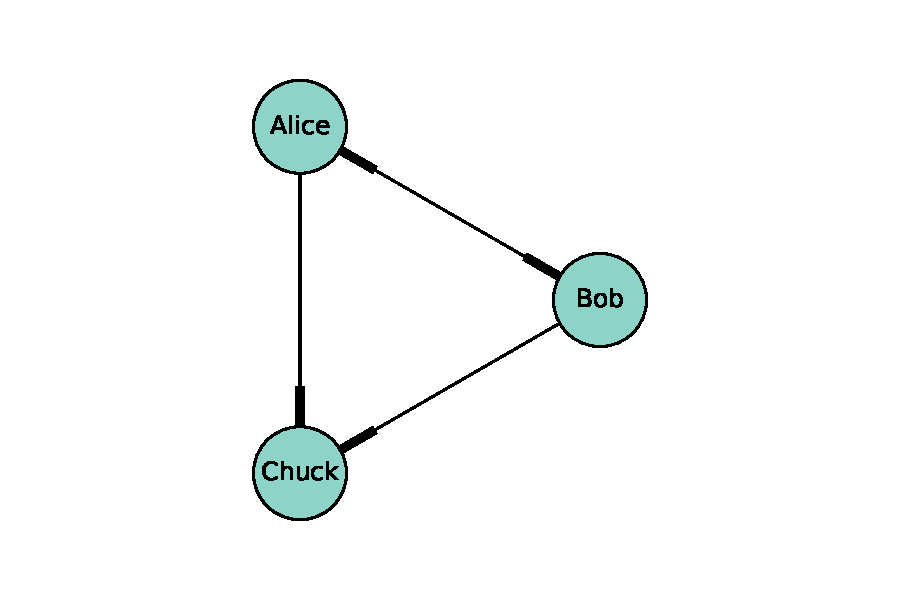
\includegraphics[width=3.5in]{figs/chap02-1.pdf}}
\caption{A directed graph that represents a social network.}
\label{chap02-1}
\end{figure}

To most people a ``graph" is a visual representation of data, like
a bar chart or a plot of stock prices over time.  That's not what this
chapter is about.  \index{graph}

In this chapter, a {\bf graph} is a representation of
a system that contains discrete, interconnected elements.  The
elements are represented by {\bf nodes}
and the interconnections are represented by {\bf edges}.
\index{node}
\index{edge}
\index{vertex}

For example, you could represent a road map with a node for each
city and an edge for each road between cities.  Or you could
represent a social network using a node for each person, with an
edge between two people if they are friends and no edge otherwise.
\index{road network}
\index{social network}

In some graphs, edges have attributes like length, cost, or weight.
For example, in a road map, the length of an edge might represent the
distance between two cities, or the travel time.  In a
social network there might be different kinds of edges to represent
different kinds of relationships: friends, business associates, etc.
\index{edge weight} \index{weight}

Edges may be {\bf directed} or {\bf undirected}, depending on whether
the relationships they represent are asymmetric or symmetric.  In a
road map, you might represent a one-way street with a directed edge
and a two-way street with an undirected edge.  In some social
networks, like Facebook, friendship is symmetric: if $A$ is friends
with $B$ then $B$ is friends with $A$.  But on Twitter, for example,
the ``follows'' relationship is not symmetric; if $A$ follows $B$,
that doesn't imply that $B$ follows $A$.  So you might use undirected
edges to represent a Facebook network and directed edges for Twitter.
\index{directed graph} \index{undirected graph}

Graphs have interesting mathematical properties, and
there is a branch of mathematics called {\bf graph theory}
that studies them.
\index{graph theory}

Graphs are also useful, because there are many real world
problems that can be solved using {\bf graph algorithms}.
For example, Dijkstra's shortest path algorithm is an efficient
way to find the shortest path from a node to all
other nodes in a graph.  A {\bf path} is a sequence of nodes
with an edge between each consecutive pair.
\index{graph algorithm}
\index{path}

Graphs are usually drawn with squares or circles for nodes and lines
for edges.  For example, the directed graph in Figure~\ref{chap02-1}
might represent three people who follow each other on Twitter.
The thick part of the line indicates edge direction.
In this example, Alice and Bob follow each other and both follow
Chuck, but Chuck follows no one.
\index{representing graphs}

The undirected graph in Figure~\ref{chap02-2} shows four cities
in the north-east United States; the labels on the edges
indicate driving time in hours.
In this example the placement of the nodes corresponds
roughly to the geography of the cities, but in general the layout
of a graph is arbitrary.
\index{graph layout}


\section{NetworkX}

\begin{figure}
\centerline{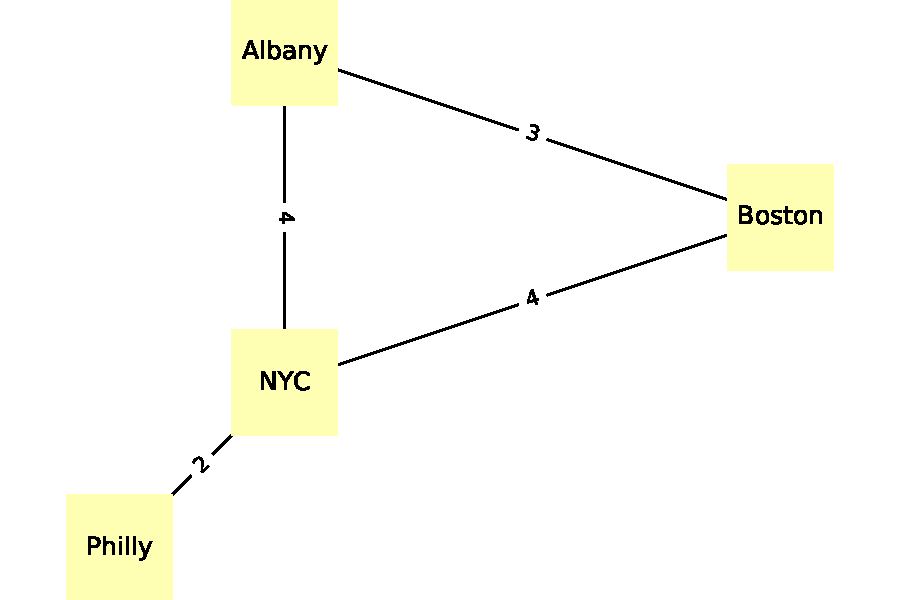
\includegraphics[width=3.5in]{figs/chap02-2.pdf}}
\caption{An undirected graph that represents cities and highways.}
\label{chap02-2}
\end{figure}

To represent graphs, we'll use a package called NetworkX,
which is the most commonly used network library in Python.
You can read more about it at \url{https://networkx.github.io/},
but I'll explain it as we go along.

We can create a directed graph by importing NetworkX (usually imported as \py{nx}) and instantiating
\py{nx.DiGraph}:

\begin{code}
import networkx as nx
G = nx.DiGraph()
\end{code}

At this point, \py{G} is a \py{DiGraph} object that contains no nodes
and no edges.  We can add nodes using the \py{add_node} method:

\begin{code}
G.add_node('Alice')
G.add_node('Bob')
G.add_node('Chuck')
\end{code}

Now we can use the \py{nodes} method to get the list of nodes:

\begin{code}
>>> G.nodes()
['Alice', 'Bob', 'Chuck']
\end{code}

Adding edges works pretty much the same way:

\begin{code}
G.add_edge('Alice', 'Bob')
G.add_edge('Alice', 'Chuck')
G.add_edge('Bob', 'Alice')
G.add_edge('Bob', 'Chuck')
\end{code}

And we can use \py{edges} to get the list of edges:

\begin{code}
>>> G.edges()
[('Alice', 'Bob'), ('Alice', 'Chuck'),
 ('Bob', 'Alice'), ('Bob', 'Chuck')]
\end{code}

NetworkX provides several functions for drawing graphs;
\py{draw_circular} arranges the nodes in a circle and connects them
with edges:

\begin{code}
nx.draw_circular(G,
                 node_color=COLORS[0],
                 node_size=2000,
                 with_labels=True)
\end{code}

And that's the code I use to generate Figure~\ref{chap02-1}.
The option \py{with_labels} causes the nodes to be labeled;
in the next example we'll see how to label the edges.

To generate Figure~\ref{chap02-2}, I start with a dictionary
that maps from each city name to its approximate longitude
and latitude:

\begin{code}
pos = dict(Albany=(-74, 43),
           Boston=(-71, 42),
           NYC=(-74, 41),
           Philly=(-75, 40))
\end{code}

Since this is an undirected graph, I instantiate \py{nx.Graph}:

\begin{code}
G = nx.Graph()
\end{code}

Then I can use \py{add_nodes_from} to iterate the keys of
\py{pos} and add them as nodes:

\begin{code}
G.add_nodes_from(pos)
\end{code}

Next I'll make a dictionary that maps from each edge to the corresponding
driving time:

\begin{code}
drive_times = {('Albany', 'Boston'): 3,
               ('Albany', 'NYC'): 4,
               ('Boston', 'NYC'): 4,
               ('NYC', 'Philly'): 2}
\end{code}

Now I can use \py{add_edges_from}, which iterates the keys of
\py{drive_times} and adds them as edges:

\begin{code}
G.add_edges_from(drive_times)
\end{code}

Now instead of \py{draw_circular}, which arranges the nodes in
a circle, I'll use \py{draw}, which takes \py{pos} as the second
parameter:

\begin{code}
nx.draw(G, pos,
        node_color=COLORS[1],
        node_shape='s',
        node_size=2500,
        with_labels=True)
\end{code}

\py{pos} is a dictionary that maps from each city to its coordinates;
\py{draw} uses it to determine the locations of the nodes.

To add the edge labels, we use \py{draw_networkx_edge_labels}:

\begin{code}
nx.draw_networkx_edge_labels(G, pos,
                             edge_labels=drive_times)
\end{code}

\py{drive_times} is a dictionary that maps from each edge, represented
by a pair of city names, to the driving distance between them.
And that's how I generated Figure~\ref{chap02-2}.

In both of these examples, the nodes are strings, but in general they
can be any hashable type.
\index{hashable}


\section{Random graphs}
\label{randomgraphs}

A random graph is just what it sounds like: a graph with nodes and edges
generated at random.  Of course, there are many random processes that
can generate graphs, so there are many kinds of random graphs.
\index{random graph}

One of the more interesting kinds is the \Erdos-\Renyi~model, studied
by Paul \Erdos~and Alfr\'{e}d \Renyi~in the 1960s.
\index{Renyi, Alfred@\Renyi, Afr\'{e}d}
\index{Erdos, Paul@\Erdos, Paul}

An \Erdos-\Renyi~graph (ER graph) is characterized by two parameters:
$n$ is the number of nodes and $p$ is the probability that there
is an edge between any two nodes.
See \url{http://en.wikipedia.org/wiki/Erdos-Renyi_model}.
\index{Erdos-Renyi model@\Erdos-\Renyi~model}

\Erdos~and \Renyi~studied the properties of these random graphs;
one of their surprising results is the existence of
abrupt changes in the properties of random graphs as
random edges are added.
\index{threshold value}

One of the properties that displays this kind of transition is
connectivity.  An undirected graph is {\bf connected} if there is a
path from every node to every other node.

In an ER graph, the probability that the graph is connected is very
low when $p$ is small and nearly 1 when $p$ is large.  Between these
two regimes, there is a rapid transition at a particular value of
$p$, denoted $p^*$.

\Erdos~and \Renyi~showed that this critical value is
$p^* = \ln n / n$, where $n$ is the number of nodes.
A random graph, $G(n, p)$, is unlikely to be connected
if $p < p^*$ and very likely to be connected if $p > p^*$.
\index{critical value}

To test this claim, we'll develop algorithms to generate random
graphs and check whether they are connected.


\section{Generating graphs}
\label{generating}

\begin{figure}
\centerline{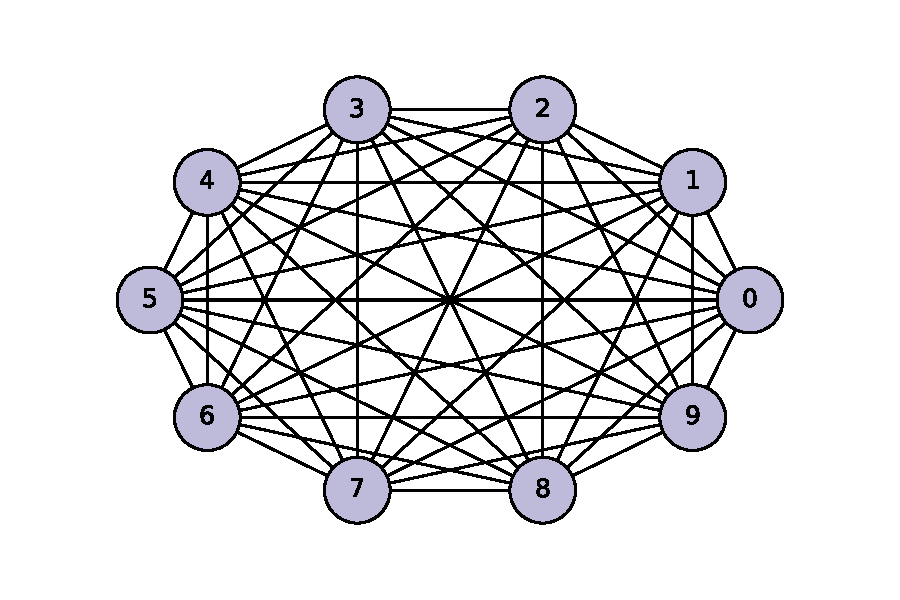
\includegraphics[width=3.5in]{figs/chap02-3.pdf}}
\caption{A complete graph with 10 nodes.}
\label{chap02-3}
\end{figure}

I'll start by generating a {\bf complete} graph, which is a graph
where every node is connected to every other.

Here's a generator function that takes a list of nodes and enumerates
all distinct pairs.  If you are not familiar with generator functions,
you can read about them at \url{http://intermediatepythonista.com/python-generators}.

\begin{code}
def all_pairs(nodes):
    for i, u in enumerate(nodes):
        for j, v in enumerate(nodes):
            if i>j:
                yield u, v
\end{code}

We can use \py{all_pairs} to construct a complete graph:

\begin{code}
def make_complete_graph(n):
    G = nx.Graph()
    nodes = range(n)
    G.add_nodes_from(nodes)
    G.add_edges_from(all_pairs(nodes))
    return G
\end{code}

\py{make_complete_graph} takes the number of nodes, \py{n}, and
returns a new \py{Graph} with \py{n} nodes and edges between all
pairs of nodes.

The following code makes a complete graph with 10 nodes and draws it.

\begin{code}
complete = make_complete_graph(10)
nx.draw_circular(complete,
                 node_color=COLORS[2],
                 node_size=1000,
                 with_labels=True)
\end{code}

Figure~\ref{chap02-3} shows the result.
Soon we will modify this code to generate ER graphs, but first
we'll develop functions to check whether a graph is connected.


\section{Connected graphs}
\label{connected}

A graph is {\bf connected} if there is a path from every node to every
other node (see \url{http://en.wikipedia.org/wiki/Connectivity_(graph_theory)}).
\index{connected graph}
\index{path}

For many applications involving graphs, it is useful to check whether a graph is connected.  Fortunately, there is a simple algorithm that does it.

You can start at any node and check whether you can reach all
other nodes.  If you can reach a node, $v$, you can reach any
of the {\bf neighbors} of $v$, which is any node connected by
$v$ by an edge.

The \py{Graph} class provides a method called \py{neighbors}
that returns a list of neighbors for a given node.  For
example, in the complete graph we generated in the previous section:

\begin{code}
>>> complete.neighbors(0)
[1, 2, 3, 4, 5, 6, 7, 8, 9]
\end{code}

Suppose we start at node $s$.  We can mark $s$ as ``seen'',
then we can mark its neighbors.
Then we mark the neighbor's neighbors, and so
on, until we can't reach any more nodes.  If all nodes are
seen, the graph is connected.

Here's what that looks like in Python:

\begin{code}
def reachable_nodes(G, start):
    seen = set()
    stack = [start]
    while stack:
        node = stack.pop()
        if node not in seen:
            seen.add(node)
            stack.extend(G.neighbors(node))
    return seen
\end{code}

\py{reachable_nodes} takes a \py{Graph} and a starting node, {\tt
  start}, and returns the set of nodes that can be reached from {\tt
  start}.

Initially the set, \py{seen}, is empty, and we create a
list called \py{stack} that keeps track of nodes we have
discovered but not yet processed.  Initially the stack contains
a single node, \py{start}.

Now, each time through the loop, we

\begin{enumerate}

\item Remove one node from the stack.

\item If the node is already in \py{seen}, we go back
to Step 1.

\item Otherwise, we add the node to \py{seen} and add its
neighbors to the stack.

\end{enumerate}

When the stack is empty, we can't reach any more nodes, so we
break out of the loop and return \py{seen}.

As an example, we can find all nodes in the complete graph that
are reachable from node 0:

\begin{code}
>>> reachable_nodes(complete, 0)
{0, 1, 2, 3, 4, 5, 6, 7, 8, 9}
\end{code}

Initially, the stack contains node 0 and \py{seen} is empty.
The first time through the loop, node 0 is added to \py{seen}
and all the other nodes are added to the stack (since they are all
neighbors of node 0).

The next time through the loop, \py{pop} returns the last element
in the stack, which is node 9.  So node 9 gets added to \py{seen}
and its neighbors get added to the stack.

Notice that the same node can appear more than once in the stack;
in fact, a node with $k$ neighbors will be added to the stack
$k$ times.  Later we will look for ways to make this algorithm
more efficient.

We can use \py{reachable_nodes} to write \py{is_connected}:

\begin{code}
def is_connected(G):
    start = next(G.nodes_iter())
    reachable = reachable_nodes(G, start)
    return len(reachable) == len(G)
\end{code}

\py{is_connected} chooses a starting node by calling
\py{nodes_iter}, which returns an iterator object, and passing the
result to \py{next}, which returns the first node.

\py{reachable} gets the set of nodes that can be reached from
\py{start}.  If the size of this set is the same as the size
of the graph, that means we can reach all nodes, which means the
graph is connected.

A complete graph is, not surprisingly, connected:

\begin{code}
>>> is_connected(complete)
True
\end{code}

In the next section we will generate ER graphs and check whether they
are connected.


\section{Generating ER graphs}

\begin{figure}
\centerline{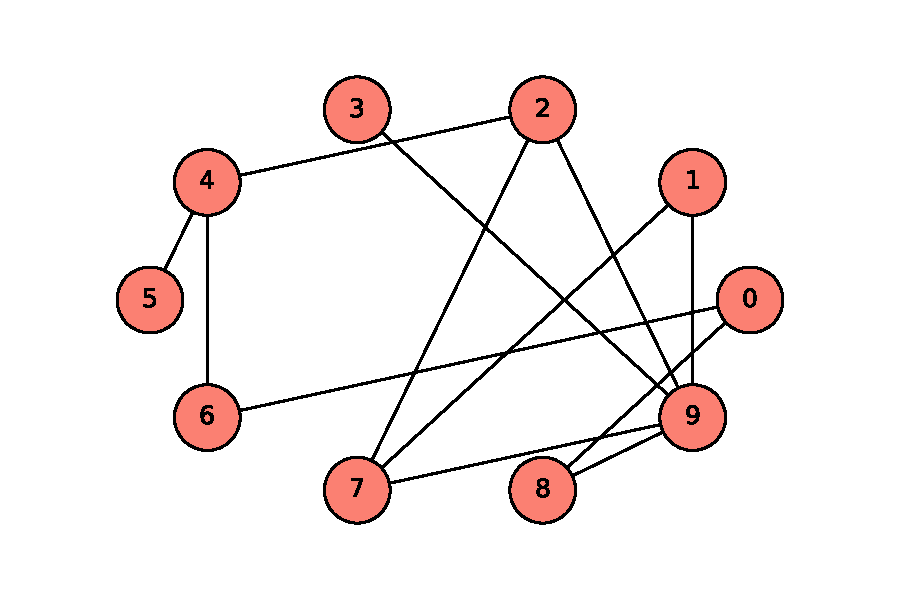
\includegraphics[width=3.5in]{figs/chap02-4.pdf}}
\caption{An ER graph with \py{n=10} and \py{p=0.3}.}
\label{chap02-4}
\end{figure}

The ER graph $G(n, p)$ contains $n$ nodes, and each pair of nodes is
connected by an edge with probability $p$.  Generating an ER graph is
similar to generating a complete graph.

The following generator function enumerates all possible edges and
uses a helper function, \py{flip}, to choose which ones should be
added to the graph:

\begin{code}
def random_pairs(nodes, p):
    for i, u in enumerate(nodes):
        for j, v in enumerate(nodes):
            if i>j and flip(p):
                yield u, v
\end{code}

\py{flip} returns \py{True} with the
given probability, \py{p}, and \py{False} with the complementary
probability \py{1-p}:

\begin{code}
from numpy.random import random

def flip(p):
    return random() < p
\end{code}

Finally, \py{make_random_graph} generates and returns the ER graph $G(n, p)$.

\begin{code}
def make_random_graph(n, p):
    G = nx.Graph()
    nodes = range(n)
    G.add_nodes_from(nodes)
    G.add_edges_from(random_pairs(nodes, p))
    return G
\end{code}

\py{make_random_graph} is almost identical to \py{make_complete_graph};
the only difference is that it uses \py{random_pairs} instead of
\py{all_pairs}.

Here's an example with \py{p=0.3}:

\begin{code}
random_graph = make_random_graph(10, 0.3)
\end{code}

Figure~\ref{chap02-4} shows the result.  This graph turns out to be
connected; in fact, most ER graphs with $n=10$ and
$p=0.3$ are connected.  In the next section, we'll see how many.



\section{Probability of connectivity}

\begin{figure}
\centerline{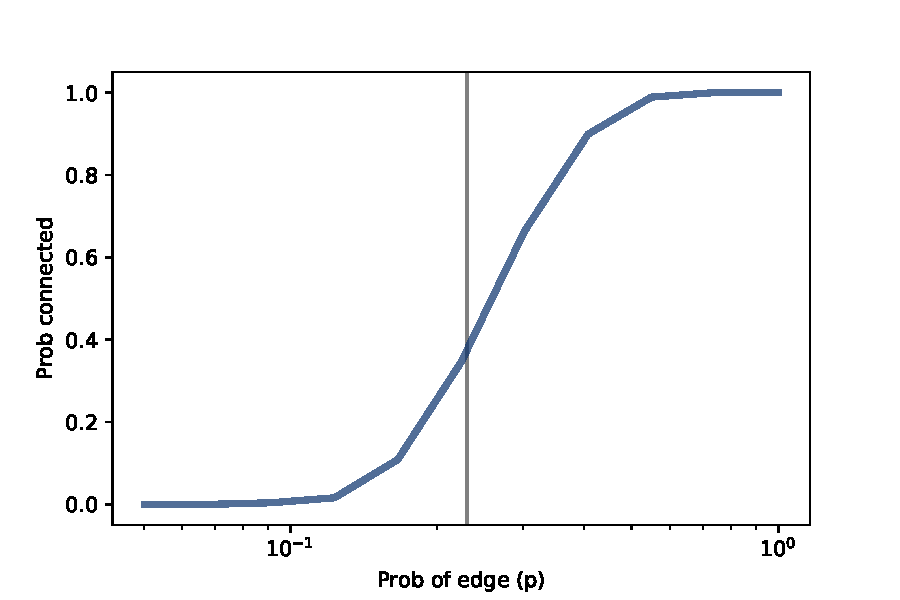
\includegraphics[width=3.5in]{figs/chap02-5.pdf}}
\caption{Probability of connectivity with $n=10$ and a range of $p$.
The vertical line shows the predicted critical value.}
\label{chap02-5}
\end{figure}

\begin{figure}
\centerline{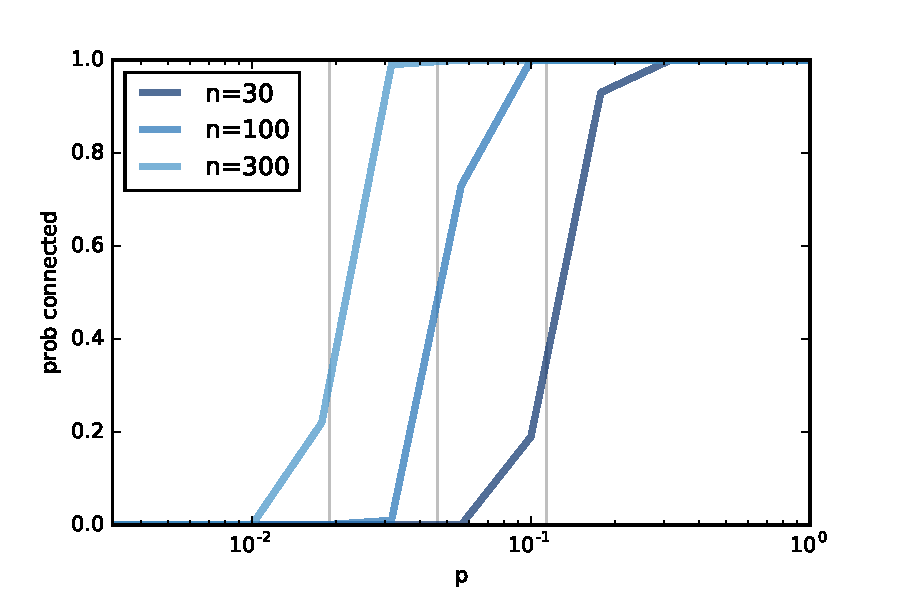
\includegraphics[width=3.5in]{figs/chap02-6.pdf}}
\caption{Probability of connectivity for several values of $n$ and a range of $p$.}
\label{chap02-6}
\end{figure}

For given values of $n$ and $p$, we would like to know the probability
that $G(n, p)$ is connected.  We can estimate it by generating
a large number of random graphs and counting how many are connected.
Here's how:

\begin{code}
def prob_connected(n, p, iters=100):
    count = 0
    for i in range(iters):
        random_graph = make_random_graph(n, p)
        if is_connected(random_graph):
            count += 1
    return count/iters
\end{code}

\py{iters} is the number of random graphs we generate.  As we
increase \py{iters}, the estimated probability gets more precise\footnote{Since \py{count} and \py{iters} are integers, this function won't work correctly in Python 2 unless you import \py{division} from \py{__future__}.  See \url{https://www.python.org/dev/peps/pep-0238/}}.

\begin{code}
>>> prob_connected(10, 0.3, iters=10000)
0.6454
\end{code}

Out of 10000 ER graphs with these parameters, 6498 are connected, so
we estimate that 65\% of them are connected.  I chose $0.3$ because it is close to the critical value where the probability of connectivity goes from near 0 to near 1.  According to \Erdos~and \Renyi, $p^* = \ln n / n = 0.23$.

We can get a clearer view of the transition by estimating the probability
of connectivity for a range of values of $p$:

\begin{code}
import numpy as np

n = 10
ps = np.logspace(-2.5, 0, 11)
ys = [prob_connected(n, p) for p in ps]
\end{code}

This is the first example we've seen using NumPy.  Following convention,
I import NumPy as {\tt np}.  The function \py{logspace} returns an
{\bf array} of 11 values from $10^{-2.5}$ to $10^0 = 1$, equally spaced
on a logarithmic scale.

To compute \py{ys}, I use a list comprehension that iterates the
elements of \py{ps} and computes the probability that a random
graph with each value of \py{p} is connected.

Figure~\ref{chap02-5} shows the results, with
a vertical line at $p^*$.  The transition from 0 to 1
occurs near the predicted critical value, 0.23.  With $p$ on a log scale,
the transition is roughly symmetric.

Figure~\ref{chap02-6} shows
similar results for larger values of $n$.  As $n$ increases, the
critical value gets smaller and the transition gets more abrupt.

These experiments are consistent with the results \Erdos~and
\Renyi~proved in their papers.


\section{Analysis of graph algorithms}
\label{graphanalysis}

In this chapter I presented an algorithm for checking whether
a graph is connected; in the next few chapters, we will see
other graph algorithms.  And we will analyze the
performance of those algorithms, figuring out how their run times
grow as the size of the graphs increases.

If you are not already familiar with analysis of algorithms,
you should read Appendix~\ref{algorithms} before you continue.

\newcommand{\V}{n}
\newcommand{\E}{m}

The order of growth for graph algorithms is usually expressed
as a function of $\V$, the number of vertices, and $\E$, the number
of edges.
\index{analysis of graph algorithms}
\index{graph algorithm}

As an example, let's analyze \py{reachable_nodes} from
Section~\ref{connected}:

\begin{code}
def reachable_nodes(G, start):
    seen = set()
    stack = [start]
    while stack:
        node = stack.pop()
        if node not in seen:
            seen.add(node)
            stack.extend(G.neighbors(node))
    return seen
\end{code}

Each time through the loop, we pop a node off the stack; by default,
\py{pop} removes and returns the last element of a list, which is
a constant time operation.

Next we check whether the node is in \py{seen}, which is a set,
so checking membership is constant time.

If the node is not already in \py{seen}, we add it, which is
constant time, and then add the neighbors to the stack, which is
linear in the number of neighbors.

To express the run time in terms of $\V$ and $\E$, we can add up
the total number of times each node is added to \py{seen}
and \py{stack}.

Each node is only added to \py{seen} once, so the total number
of additions is $\V$.

But nodes might be added to \py{stack} many times, depending on
how many neighbors they have.  If a node has $k$ neighbors, it
is added to \py{stack} $k$ times.  Of course, if it has $k$ neighbors,
that means it is connected to $k$ edges.

So the total number
of additions to \py{stack} is the total number of edges, $\E$,
doubled because we consider every edge twice.

Therefore, the order of growth for this function is $O(\V + \E)$,
which is a convenient way to say that the run time grows in proportion
to either $\V$ or $\E$, whichever is bigger.
\index{breadth first search} \index{BFS}

If we know the relationship between $\V$ and $\E$, we can simplify
this expression.  For example, in a complete graph the number of edges
is $n(n-1)/2$, which is in $O(\V^2)$.  So for a complete graph,
\py{reachable_nodes} is quadratic in $\V$.
\index{quadratic}


\section{Exercises}

The code for this chapter is in \py{chap02.ipynb}, which is a
Jupyter notebook in the repository for this book.  For more information
about working with this code, see Section~\ref{code}.

\begin{exercise}
Launch \py{chap02.ipynb} and run the code.  There are a few short
exercises embedded in the notebook that you might want to try.
\end{exercise}

\begin{exercise}
In Section~\ref{graphanalysis} we analyzed the performance of
\py{reachable_nodes} and classified it in $O(n + m)$, where $n$ is the
number of nodes and $m$ is the number of edges.  Continuing the
analysis, what is the order of growth for \py{is_connected}?

\begin{code}
def is_connected(G):
    start = next(G.nodes_iter())
    reachable = reachable_nodes(G, start)
    return len(reachable) == len(G)
\end{code}


\end{exercise}

\begin{exercise}
In my implementation of \py{reachable_nodes}, you might be bothered by
the apparent inefficiency of adding {\em all} neighbors to the stack
without checking whether they are already in \py{seen}.  Write a
version of this function that checks the neighbors before adding them
to the stack.  Does this ``optimization'' change the order of growth?
Does it make the function faster?
\end{exercise}


\begin{exercise}

There are actually two kinds of ER graphs.  The one we generated in
this chapter, $G(n, p)$, is characterized by two parameters, the number
of nodes and the probability of an edge between nodes.

An alternative definition, denoted $G(n, m)$, is also characterized by
two parameters: the number of nodes, $n$, and the number of edges,
$m$.  Under this definition, the number of edges is fixed, but their
location is random.

Repeat the experiments we did in this chapter using this alternative
definition.  Here are a few suggestions for how to proceed:

1. Write a function called \py{m_pairs} that takes a list of nodes
and the number of edges, $m$, and returns a random selection of $m$
edges.  A simple way to do that is to generate a list of all possible
edges and use \py{random.sample}.

2. Write a function called \py{make_m_graph} that takes $n$ and
$m$ and returns a random graph with $n$ nodes and $m$ edges.

3. Make a version of \py{prob_connected} that uses
\py{make_m_graph} instead of \py{make_random_graph}.

4. Compute the probability of connectivity for a range of values of $m$.

How do the results of this experiment compare to the results using the
first type of ER graph?

\end{exercise}


\chapter{Small world graphs}

Many networks in the real world, including social networks, have
the ``small world property'', which is that the average distance
between nodes, measured in number of edges on the shortest path,
is much smaller than expected.

In this chapter, I present Stanley Milgram's famous Small World
Experiment, which was the first scientific demonstration of
the small world property in a real social network.  Then we'll
consider Watts-Strogatz graphs, which are intended as a model of
small world graphs.
I'll replicate the experiment Watts and Strogatz performed and
explain what it is intended to show.

Along the way, we'll see two new graph algorithms: breadth-first
search (BFS) and Dijkstra's algorithm for computing the shortest
path between nodes in a graph.

The code for this chapter is in {\tt chap03.ipynb} in the repository
for this book.  More information about working with the code is
in Section~\ref{code}.

\section{Stanley Milgram}

Stanley Milgram was an American social psychologist who conducted
two of the most famous experiments in social science, the
Milgram experiment, which studied people's obedience to authority
(\url{http://en.wikipedia.org/wiki/Milgram_experiment})
and the Small World Experiment, which studied
the structure of social networks
(\url{http://en.wikipedia.org/wiki/Small_world_phenomenon}).
\index{Milgram, Stanley}
\index{small world experiment}

In the Small World Experiment, Milgram sent a package to several
randomly-chosen people in Wichita, Kansas, with instructions asking
them to forward an enclosed letter to a target person, identified by
name and occupation, in Sharon, Massachusetts (which is the town near
Boston where I grew up).  The subjects were told that they could mail
the letter directly to the target person only if they knew him
personally; otherwise they were instructed to send it, and the same
instructions, to a relative or friend they thought would be more
likely to know the target person.
\index{Kansas}
\index{Wichita, Kansas}
\index{Massachusetts}
\index{Sharon, Massachusetts}

Many of the letters were never delivered, but for the ones that
were the average path length---the number of
times the letters were forwarded---was about six.  This result
was taken to confirm previous observations (and speculations) that
the typical distance between any two people in a social network
is about ``six degrees of separation.''
\index{six degrees}

This conclusion is surprising because most people expect social
networks to be localized---people tend to live near their
friends---and in a graph with local connections, path lengths tend to
increase in proportion to geographical distance.  For example, most of
my friends live nearby, so I would guess that the average distance
between nodes in a social network is about 50 miles.  Wichita is about
1600 miles from Boston, so if Milgram's letters traversed typical
links in the social network, they should have taken 32 hops, not six.
\index{hop}
\index{social network}
\index{local connection}


\section{Watts and Strogatz}

In 1998 Duncan Watts and Steven Strogatz published a paper in {\em
  Nature}, ``Collective dynamics of `small-world' networks'', that
proposed an explanation for the small world phenomenon.  You can
download it from
\url{http://www.nature.com/nature/journal/v393/n6684/abs/393440a0.html}.
\index{Watts, Duncan} \index{Strogatz, Steven} \index{small world
  network}

Watts and Strogatz start with two kinds of graph that were well
understood: random graphs and regular graphs.  In a random graph, nodes
are connected at random.  In a regular graph, every node has the
same number of neighbors.
They consider two
properties of these graphs, clustering and path length:
\index{random graph}
\index{regular graph}
\index{clustering}
\index{path length}

\begin{description}

\item Clustering is a measure of the ``cliquishness'' of the graph.
In a graph, a {\bf clique} is a subset of nodes that are
all connected to each other; in a social network, a clique is
a set of people who are all friends with each other.  Watts and Strogatz
defined a clustering coefficient that quantifies the likelihood
that two nodes that are connected to the same node are also
connected to each other.
\index{clique}

\item Path length is a measure of the average distance between
two nodes, which corresponds to the degrees of separation in
a social network.

\end{description}

Watts and Strogatz show that regular graphs
have high clustering and high path lengths, whereas
random graphs with the same size usually have low clustering
and low path lengths.  So neither of these is a good model of
social networks, which combine high clustering with
short path lengths.

Their goal was to create a {\bf generative model} of a social
network.  A generative model tries to explain a phenomenon by
modeling the process that builds or leads to the phenomenon.
Watts and Strogatz proposed this process for building
small-world graphs:
\index{generative model}

\begin{enumerate}

\item Start with a regular graph with $n$ nodes and each node
  connected to $k$ neighbors.

\item Choose a subset of the edges and ``rewire'' them by
  replacing them with random edges.
  \index{rewire}

\end{enumerate}

The probability that an edge is rewired is a parameter, $p$,
that controls how random the graph is.  With $p=0$, the graph
is regular; with $p=1$ it is random.
\index{parameter}

Watts and Strogatz found that small values of $p$ yield graphs
with high clustering, like a regular graph, and low path
lengths, like a random graph.

In this chapter I replicate the Watts and Strogatz experiment
in the following steps:

\begin{enumerate}

\item We'll start by constructing a ring lattice, which is a kind
of regular graph.

\item Then we'll rewire it as Watts and Strogatz did.

\item We'll write a function to measure the degree of clustering
and use a NetworkX function to compute path lengths.

\item Then we'll compute the degree of clustering and path length for
a range of values of $p$.

\item Finally, I'll present an efficient algorithm for computing shortest
paths, Dijkstra's algorithm.

\end{enumerate}


\section{Ring lattice}

\begin{figure}
\centerline{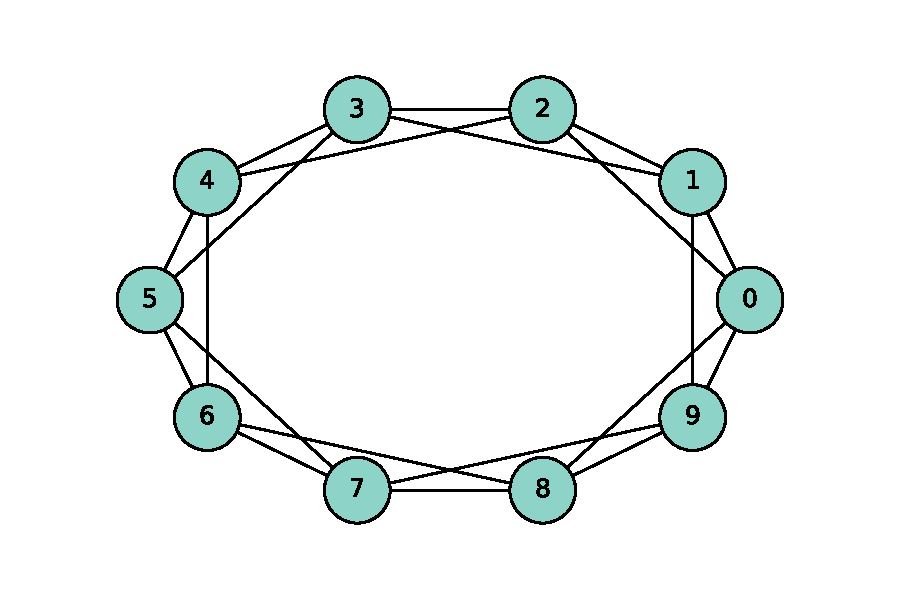
\includegraphics[width=3.5in]{figs/chap03-1.pdf}}
\caption{A ring lattice with $n=10$ and $k=4$.}
\label{chap03-1}
\end{figure}

A {\bf regular} graph is a graph where each node has the same number
of neighbors; the number of neighbors is also called the {\bf degree}
of the node.

A ring lattice is a kind of regular graph, which Watts and Strogatz
use as the basis of their model.
In a ring lattice with $n$ nodes, the nodes can be arranged in a circle
with each node connected to the $k$ nearest neighbors.

For example, a ring lattice with $n=3$
and $k=2$ would add the following edges: $(0, 1)$, $(1, 2)$, and
$(2, 0)$.  Notice that the edges ``wrap around'' from the
highest-numbered node back to 0.

More generally, we can enumerate the edges like this:

\begin{code}
def adjacent_edges(nodes, halfk):
    n = len(nodes)
    for i, u in enumerate(nodes):
        for j in range(i+1, i+halfk+1):
            v = nodes[j % n]
            yield u, v
\end{code}

\py{adjacent_edges} takes a list of nodes and a parameter,
\py{halfk}, which is half of $k$.  It is a generator function that
yields one edge at a time.  It uses the modulus operator, \verb"%",
to wrap around from the highest-numbered node to the lowest.

We can test it like this:

\begin{code}
>>> nodes = range(3)
>>> for edge in adjacent_edges(nodes, 1):
...     print(edge)
(0, 1)
(1, 2)
(2, 0)
\end{code}

Now we can use \py{adjacent_edges} to make a ring lattice:

\begin{code}
def make_ring_lattice(n, k):
    G = nx.Graph()
    nodes = range(n)
    G.add_nodes_from(nodes)
    G.add_edges_from(adjacent_edges(nodes, k//2))
    return G
\end{code}

Notice that \py{make_ring_lattice} uses floor division to compute
\py{halfk}, so if \py{k} is odd, it will round down and generate
a ring lattice with degree \py{k-1}.  That's probably not what we
want, but it is good enough for now.

We can test the function like this:

\begin{code}
lattice = make_ring_lattice(10, 4)
\end{code}

Figure~\ref{chap03-1} shows the result.


\section{WS graphs}

\begin{figure}
\centerline{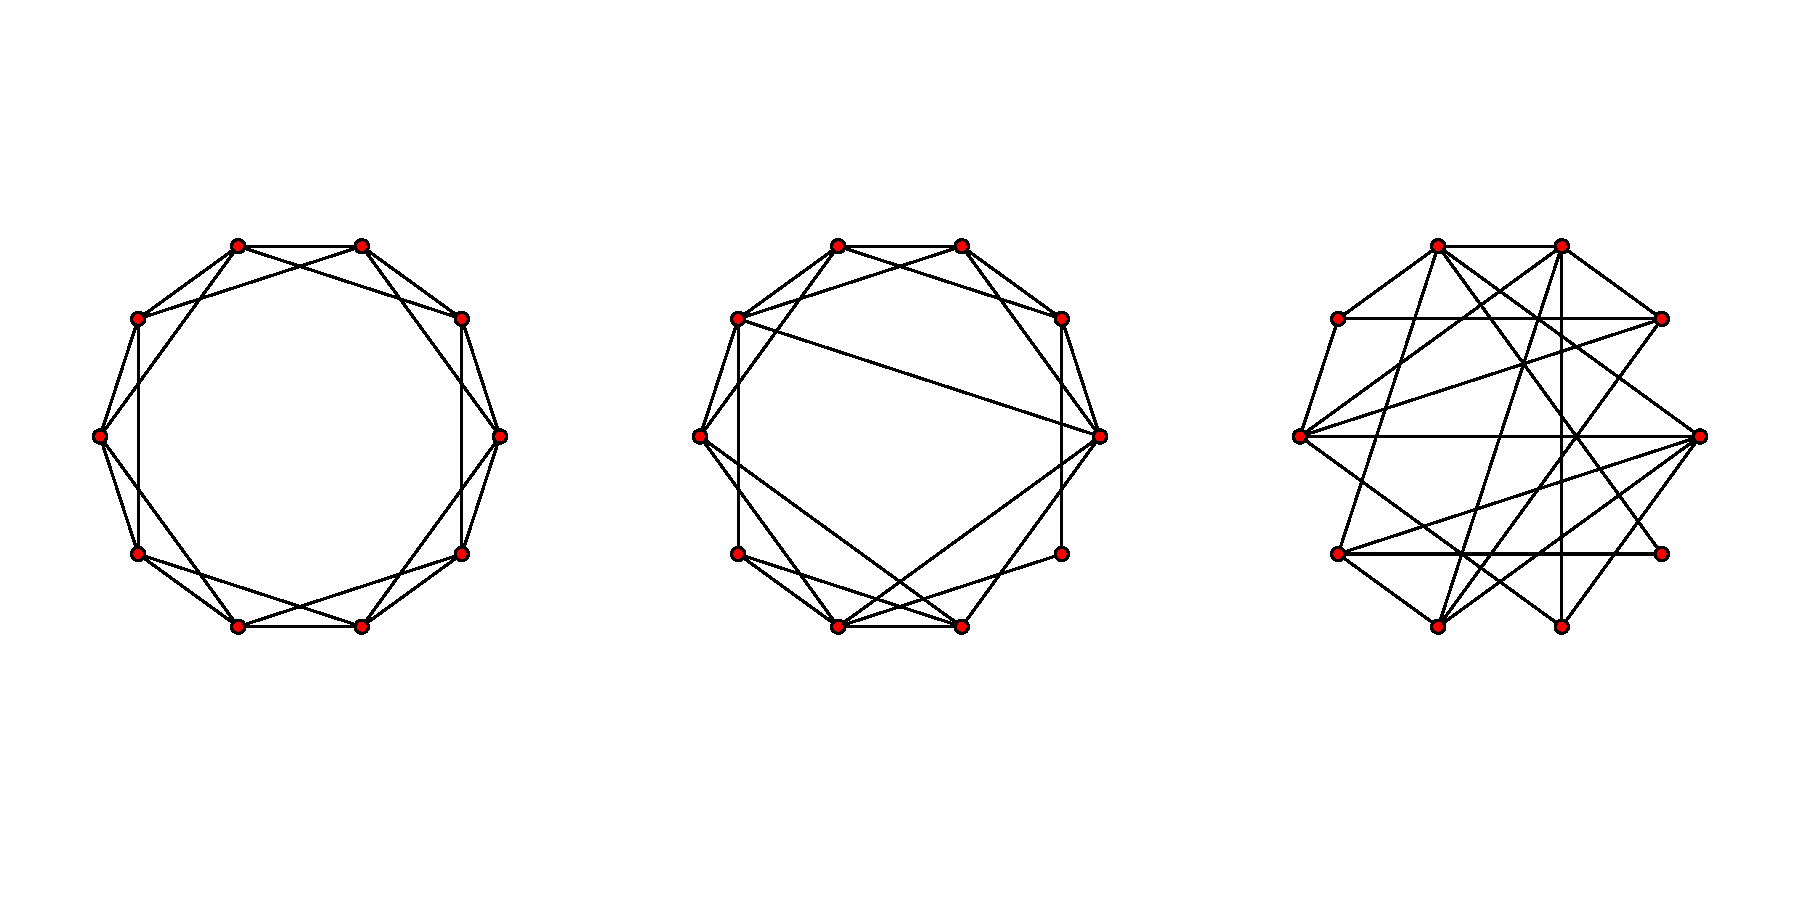
\includegraphics[width=3.5in]{figs/chap03-2.pdf}}
\caption{WS graphs with $n=20$, $k=4$, and $p=0$ (left), $p=0.2$ (middle),
and $p=1$ (right).}
\label{chap03-2}
\end{figure}

To make a Watts-Strogatz (WS) graph, we start with a ring lattice and
``rewire'' some of the edges.  In their paper, Watts and Strogatz
consider the edges in a particular order and rewire each one with
probability $p$.  If an edge is rewired, they leave the first node
unchanged and choose the second node at random.  They don't allow self
loops or multiple edges; that is, you can't have a edge from a node to
itself, and you can't have more than one edge between the same two
nodes.

Here is my implementation of this process.

\begin{code}
def rewire(G, p):
    nodes = set(G.nodes())
    for edge in G.edges():
        if flip(p):
            u, v = edge
            choices = nodes - {u} - set(G[u])
            new_v = choice(tuple(choices))
            G.remove_edge(u, v)
            G.add_edge(u, new_v)
\end{code}

The parameter \py{p} is the probability of rewiring an edge.  The
\py{for} loop enumerates the edges and uses \py{flip}, which returns
\py{True} with probability \py{p}, to choose which ones get rewired.

If we are rewiring an edge from node \py{u} to node \py{v}, we
have to choose a replacement for \py{v}, called \py{new_v}.
To compute the possible choices,
we start with \py{nodes}, which is a set,
and subtract off \py{u} and its neighbors, which avoids self
loops and multiple edges.

Then we choose \py{new_v} from \py{choices}, remove the existing
edge from \py{u} to \py{v}, and add a new edge from \py{u} to
\py{new_v}.

As an aside, the expression \py{G[u]} returns a
dictionary that contains the neighbors of \py{u} as keys.  In
this case it is a little faster than using \py{G.neighbors}.

This function does not consider the edges in the order specified
by Watts and Strogatz, but it doesn't seem to affect
the results.

Figure~\ref{chap03-2} shows WS graphs with $n=20$, $k=4$, and
a range of values of $p$.  When $p=0$, the graph is a ring lattice.
When $p=1$, it is completely random.  As we'll see, the interesting
things happen in between.


\section{Clustering}
\label{clustering}

The next step is to compute the clustering coefficient, which
quantifies the tendency for the nodes to form cliques.
A {\bf clique} is a set of nodes that are completely connected;
that is, there are edges between all pairs of nodes in the set.

Suppose a particular node, $u$, has $k$ neighbors.  If all of the
neighbors are connected to each other, there would be $k(k-1)/2$
edges among them.  The fraction of those edges that actually exist
is the local clustering coefficient for $u$, denoted $C_u$.
It is called
a ``coefficient'' because it is always between 0 and 1.

If we compute the average of $C_u$ over all nodes, we get the
``network average clustering coefficient'', denoted $\bar{C}$.

Here is a function that computes it.

\begin{code}
def node_clustering(G, u):
    neighbors = G[u]
    k = len(neighbors)
    if k < 2:
        return 0

    total = k * (k-1) / 2
    exist = 0
    for v, w in all_pairs(neighbors):
        if G.has_edge(v, w):
            exist +=1
    return exist / total
\end{code}

Again I use \py{G[u]}, which returns a dictionary
with the neighbors of \py{node} as keys.  If a node has fewer than 2
neighbors, the clustering coefficient is undefined, but for simplicity
\py{node_clustering} returns 0.

Otherwise we compute the number of possible edges among the neighbors,
\py{total}, and then count the number of those edges that actually
exist.  The result is the fraction of all edges that exist.

We can test the function like this:

\begin{code}
>>> lattice = make_ring_lattice(10, 4)
>>> node_clustering(lattice, 1)
0.5
\end{code}

In a ring lattice with $k=4$, the clusting coefficient for each node
is 0.5 (if you are not convinced, take another look at
Figure~\ref{chap03-1}).

Now we can compute the network average clustering coefficient like this:

\begin{code}
def clustering_coefficient(G):
    cc = np.mean([node_clustering(G, node) for node in G])
    return cc
\end{code}

\py{np.mean} is a NumPy function that computes the mean of the numbers
in a list or array.

And we can test it like this:

\begin{code}
>>> clustering_coefficient(lattice)
0.5
\end{code}

In this graph, the local clustering coefficient for all nodes is 0.5,
so the average across nodes is 0.5.  Of course, we expect this value
to be different for WS graphs.


\section{Shortest path lengths}
\label{pathlength}

The next step is to compute the characteristic path length, $L$, which
is the average length of the shortest path between each pair of nodes.
To compute it, I'll start with a function provided by NetworkX,
\py{shortest_path_length}.  I'll use it to replicate the Watts and
Strogatz experiment, then I'll explain how it works.

Here's a function that takes a graph and returns a list of shortest
path lengths, one for each pair of nodes.

\begin{code}
def path_lengths(G):
    length_map = nx.shortest_path_length(G)
    lengths = [length_map[u][v] for u, v in all_pairs(G)]
    return lengths
\end{code}

The return value from \py{nx.shortest_path_length} is a dictionary
of dictionaries.  The outer dictionary maps from each node, \py{u},
to a dictionary that maps from each node, \py{v}, to the length of
the shortest path from \py{u} to \py{v}.

With the list of lengths from \py{path_lengths}, we can compute $L$
like this:

\begin{code}
def characteristic_path_length(G):
    return np.mean(path_lengths(G))
\end{code}

And we can test it with a small ring lattice:

\begin{code}
>>> lattice = make_ring_lattice(3, 2)
>>> characteristic_path_length(lattice)
1.0
\end{code}

In this example, all 3 nodes are connected to each other, so the
mean path length is 1.


\section{The WS experiment}

\begin{figure}
\centerline{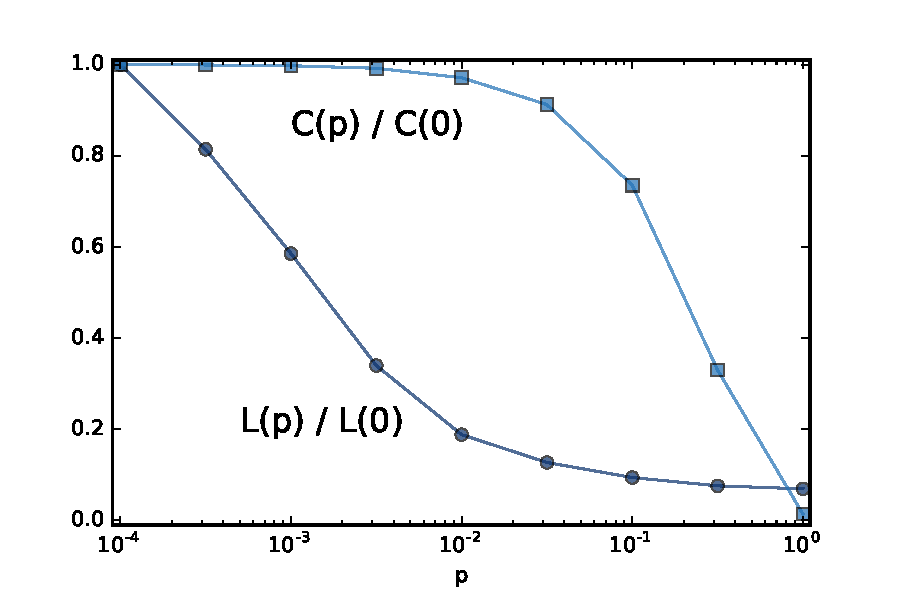
\includegraphics[width=3.5in]{figs/chap03-3.pdf}}
\caption{Clustering coefficient (C) and characteristic path length (L) for
WS graphs with $n=1000$, $k=10$, and a range of $p$.}
\label{chap03-3}
\end{figure}

Now we are ready to replicate the WS experiment, which shows that for
a range of values of $p$, a WS graph has high clustering like a
regular graph and short path lengths like a random graph.

I'll start with \py{run_one_graph}, which takes \py{n}, \py{k}, and \py{p}; it
generates a WS graph with the given parameters and computes the
mean path length, \py{mpl}, and clustering coefficient \py{cc}:

\begin{code}
def run_one_graph(n, k, p):
    ws = make_ws_graph(n, k, p)
    mpl = characteristic_path_length(ws)
    cc = clustering_coefficient(ws)
    print(mpl, cc)
    return mpl, cc
\end{code}

Watts and Strogatz ran their experiment with \py{n=1000} and \py{k=10}.
With these parameters, \py{run_one_graph} takes about one second on
my computer; most of that time is spent computing the
mean path length.

Now we need to compute these values for a range of \py{p}.  I'll use
the NumPy function \py{logspace} again to compute \py{ps}:

\begin{code}
ps = np.logspace(-4, 0, 9)
\end{code}

For each value of \py{p}, I generate 3 random graphs and we'll average the
results.  Here's the function that runs the experiment:

\begin{code}
def run_experiment(ps, n=1000, k=10, iters=3):
    res = {}
    for p in ps:
        print(p)
        res[p] = []
        for _ in range(iters):
            res[p].append(run_one_graph(n, k, p))
    return res
\end{code}

The result is a dictionary that maps from each value of \py{p} to
a list of \py{(mpl, cc)} pairs.

The last step is to aggregate the results:

\begin{code}
L = []
C = []
for p, t in sorted(res.items()):
    mpls, ccs = zip(*t)
    mpl = np.mean(mpls)
    cc = np.mean(ccs)
    L.append(mpl)
    C.append(cc)
\end{code}

Each time through the loop, we get a value of \py{p} and a list of
\py{(mpl, cc)} pairs.  We use \py{zip} to extracts two lists, \py{mpls} and
\py{ccs}, then compute their means and append them to \py{L} and \py{C}, which
are lists of path lengths and clustering coefficients.

In order to plot \py{L} and \py{C} on the same axes, we standardize them
by dividing through by the first element:

\begin{code}
L = np.array(L) / L[0]
C = np.array(C) / C[0]
\end{code}

Figure~\ref{chap03-3} shows the results.  As $p$ increases, the mean
path length drops quickly, because even a small number of randomly
rewired edges provide shortcuts between regions of the graph that
are far apart in the lattice.  On the other hand, removing local links
decreases the clustering coefficient, but much more slowly.

As a result, there is a wide range of $p$ where a WS graph has the
properties of a small world graph, high clustering and low path
lengths.

And that's why Watts and Strogatz propose WS graphs as a
model for real-world networks that exhibit the small world phenomenon.


\section{What kind of explanation is {\em that}?}

If you ask me why planetary orbits are elliptical,
I might start by modeling a planet and a star as point masses; I
would look up the law of universal gravitation at
\url{http://en.wikipedia.org/wiki/Newton's_law_of_universal_gravitation}
and use it to write a differential equation for the motion of
the planet.  Then I would either derive the orbit equation or,
more likely, look it up at \url{http://en.wikipedia.org/wiki/Orbit_equation}.
With a little algebra, I could derive the conditions that
yield an elliptical orbit.  Then I would argue that the objects
we consider planets satisfy these conditions.
\index{planetary motion}
\index{universal gravitation}

People, or at least scientists, are generally satisfied with
this kind of explanation.  One of the reasons for its appeal
is that the assumptions and approximations in the model seem
reasonable.  Planets and stars are not really point masses,
but the distances between them are so big that their actual
sizes are negligible.  Planets in the same solar system can
affect each others' orbits, but the effect is usually small.
And we ignore relativistic effects, again on the assumption that
they are small.
\index{explanatory model}

This explanation is also appealing because it is equation-based.
We can express the orbit equation in a closed form, which means
that we can compute orbits efficiently.  It also means that
we can derive general expressions for the orbital velocity,
orbital period, and other quantities.
\index{equation-based model}

Finally, I think this kind of explanation is appealing because
it has the form of a mathematical proof.  It starts from a
set of axioms and derives the result by logic and analysis.
But it is important to remember that the proof pertains to the
model and not the real world.  That is, we can prove that
an idealized model of a planet yields an elliptic orbit, but
we can't prove that the model pertains to actual planets (in
fact, it does not).
\index{mathematical proof}
\index{proof}

By comparison, Watts and Strogatz's explanation of the small
world phenomenon may seem less satisfying.  First, the model
is more abstract, which is to say less realistic.  Second,
the results are generated by simulation, not by mathematical
analysis.  Finally, the results seem less like a proof and
more like an example.
\index{abstract model}

Many of the models in this book are like the Watts and Strogatz model:
abstract, simulation-based and (at least superficially) less formal
than conventional mathematical models.  One of the goals of this book
it to consider the questions these models raise:

\index{simulation-based model}

\begin{itemize}

\item What kind of work can these models do: are they predictive, or
  explanatory, or both?

\item Are the explanations these models offer less satisfying than
  explanations based on more traditional models?  Why?

\item How should we characterize the differences between these and
  more conventional models?  Are they different in kind or only in
  degree?

\end{itemize}

Over the course of the book I will offer my answers
to these questions, but they are tentative and sometimes
speculative.  I encourage you to consider them skeptically
and reach your own conclusions.


\section{Breadth-First Search}
\label{bfs}

When we computed shortest paths, we used a function provided by
NetworkX, but I have not explained how it works.  To do that, I'll
start with breadth-first search, which is the basis of Dijkstra's
algorithm for computing shortest paths.

In Section~\ref{connected} I presented \py{reachable_nodes}, which finds all
the nodes that can be reached from a given starting node:

\begin{code}
def reachable_nodes(G, start):
    seen = set()
    stack = [start]
    while stack:
        node = stack.pop()
        if node not in seen:
            seen.add(node)
            stack.extend(G.neighbors(node))
    return seen
\end{code}

I didn't say so at the time, but \py{reachable_nodes} performs a
depth-first search (DFS).  Now we'll modify it to perform breadth-first
search (BFS).

To understand the difference, imagine you are exploring a castle.
You start in a room with three doors marked A, B, and C.  You open
door C and discover another room, with doors marked D, E, and F.

Which door do you open next?  If you are feeling adventurous, you might
want to go deeper into the castle and choose D, E, or F.  That would be
a depth-first search.

But if you wanted to be more systematic, you might go back and explore
A and B before D, E, and F.  That would be a breadth-first search.

In \py{reachable_nodes}, we use \py{list.pop} to choose the next node to
``explore''.  By default, \py{pop} returns the last element of the list,
which is the last one we added.  In the example, that would be door F.

If we want to perform a BFS instead, the simplest solution is to
pop the first element off the stack:

\begin{code}
        node = stack.pop(0)
\end{code}

That works, but it is slow.  In Python, popping the last element
of a list takes constant time, but popping the first element is linear
in the length of the list.  In the worst case, the length of the
stack is $O(\V)$, which makes this implementation of BFS $O(\V\E)$,
which is much worse than what it should be, $O(\V + \E)$.

We can solve this problem with a double-ended queue, also known
as a {\bf deque}.  The important feature of a deque is that you
can add and remove elements from the beginning or end in constant time.
To see how it is implemented, see \url{https://en.wikipedia.org/wiki/Double-ended_queue}.

Python provides a \py{deque} in the \py{collections} module, so we can
import it like this:

\begin{code}
from collections import deque
\end{code}

And we can use it to write an efficient BFS:

\begin{code}
def reachable_nodes_bfs(G, start):
    seen = set()
    queue = deque([start])
    while queue:
        node = queue.popleft()
        if node not in seen:
            seen.add(node)
            queue.extend(G.neighbors(node))
    return seen
\end{code}

The differences are:

\begin{itemize}

\item I replaced the list called \py{stack} with a deque called \py{queue}.

\item I replaced \py{pop} with \py{popleft}, which removes and returns
leftmost element of the queue, which was the first to be added.

\end{itemize}

This version is back to being $O(\V + \E)$.  Now we're ready to
find shortest paths.


\section{Dijkstra's algorithm}
\label{dijkstra}

Edsger W. Dijkstra was a Dutch computer scientist who invented an
efficient shortest-path algorithm (see
\url{http://en.wikipedia.org/wiki/Dijkstra's_algorithm}).  He also invented the
semaphore, which is a data structure used to coordinate programs that
communicate with each other (see
\url{http://en.wikipedia.org/wiki/Semaphore_(programming)} and Downey, {\em The
  Little Book of Semaphores}).

\index{Dijkstra, Edsger}
\index{Little Book of Semaphores@{\em The Little Book of Semaphores}}

Dijkstra is famous (and notorious) as the author of a series
of essays on computer science.
Some, like ``A Case against the GO TO Statement'', have
had a profound effect on programming practice.
Others, like
``On the Cruelty of Really Teaching Computing Science'', are
entertaining in their cantankerousness, but less effective.

{\bf Dijkstra's algorithm} solves the ``single source shortest path
problem'', which means that it finds the minimum distance from a given
``source'' node to every other node in the graph (or at least every
connected node).

\index{shortest path}
\index{single source shortest path}
\index{Dijkstra's algorithm}

We start with a simplified version of the algorithm that
considers all edges the same length.  The more general version
works with any non-negative edge lengths.

The simplified version is similar to the breadth-first search
in Section~\ref{bfs} except that we replace the set called
\py{seen} with a dictionary called \py{dist}, which maps from each
node to its distance from the source:

%TODO: get rid of the second set constructor, if possible

\begin{code}
def shortest_path_dijkstra(G, start):
    dist = {start: 0}
    queue = deque([start])
    while queue:
        node = queue.popleft()
        new_dist = dist[node] + 1

        neighbors = set(G[node]) - set(dist)
        for n in neighbors:
            dist[n] = new_dist

        queue.extend(neighbors)
    return dist
\end{code}

Here's how it works:

\begin{itemize}

\item Initially, \py{queue} contains a single element, \py{start}, and \py{dist}
maps from \py{start} to distance 0 (which is the distance from \py{start} to
itself).

\item Each time through the loop, we use \py{popleft} to select nodes
in the order they were added to the queue.

\item Next we find all neighbors of \py{node} that are not already in
\py{dist}.

\item Since the distance from \py{start} to \py{node} is \py{dist[node]}, the
distance to any of the undiscovered neighbors is \py{dist[node]+1}.

\item For each neighbor, we add an entry to \py{dist}, then we add
the neighbors to the queue.

\end{itemize}

This algorithm only works if we use BFS, not DFS.  Why?

The first time through the loop \py{node} is \py{start}, and \py{new_dist}
is 1.  So the neighbors of \py{start} get distance 1 and they
go in the queue.

When we process the neighbors of \py{start}, all of {\em their}
neighbors get distance 2.  We know that none of them can have
distance 1, because if they did, we would have discovered
them during the first iteration.

Similarly, when we process the nodes with distance 2, we give
their neighbors distance 3.  We know that none of them can
have distance 1 or 2, because if they did, we would have
discovered them during a previous iteration.

And so on.  If you are familiar with proof by induction, you
can see where this is going.

But this argument only works if we process all nodes with distance
1 before we start processing nodes with distance 2, and so on.
And that's exactly what BFS does.

In the exercises at the end of this chapter, you'll write a version
of Dijkstra's algorithm using DFS, so you'll have a chance to see
what goes wrong.


\section{Exercises}

\begin{exercise}

In a ring lattice, every node has the same number of neighbors.  The
number of neighbors is called the {\bf degree} of the node, and a
graph where all nodes have the same degree is called a {\bf regular
  graph}.

All ring lattices are regular, but not all regular graphs are ring
lattices.  In particular, if \py{k} is odd, we can't construct a ring
lattice, but we might be able to construct a regular graph.

Write a function called \py{make_regular_graph} that takes \py{n} and \py{k}
and returns a regular graph that contains \py{n} nodes, where every node
has \py{k} neighbors.  If it's not possible to make a regular graph with
the given values of \py{n} and \py{k}, the function should raise a
\py{ValueError}.

\end{exercise}


\begin{exercise}

My implementation of \py{reachable_nodes_bfs} is efficient in the sense
that it is in $O(\V + \E)$, but it incurs a lot of overhead adding nodes
to the queue and removing them.  NetworkX provides a simple, fast
implementation of BFS, available from the NetworkX repository on
  GitHub at \url{https://github.com/networkx/networkx/blob/master/networkx/algorithms/components/connected.py}.

%TODO: tinyurl

Here is a version I modified to return a set of nodes:

\begin{code}
def _plain_bfs(G, source):
    seen = set()
    nextlevel = {source}
    while nextlevel:
        thislevel = nextlevel
        nextlevel = set()
        for v in thislevel:
            if v not in seen:
                seen.add(v)
                nextlevel.update(G[v])
    return seen
\end{code}

Compare this function to \py{reachable_nodes_bfs} and see which is
faster.  Then see if you can modify this function to implement a
faster version of \py{shortest_path_dijkstra}.

\end{exercise}


\begin{exercise}

The following implementation of a BFS
contains two performance errors.  What are
they?  What is the actual order of growth for this algorithm?
\index{order of growth}
\index{performance error}

\begin{code}
def bfs(top_node, visit):
    """Breadth-first search on a graph, starting at top_node."""
    visited = set()
    queue = [top_node]
    while len(queue):
        curr_node = queue.pop(0)    # Dequeue
        visit(curr_node)            # Visit the node
        visited.add(curr_node)

        # Enqueue non-visited and non-enqueued children
        queue.extend(c for c in curr_node.children
                     if c not in visited and c not in queue)
\end{code}

\end{exercise}


\begin{exercise}
In Section~\ref{dijkstra}, I claimed that Dijkstra's algorithm does
not work unless it uses BFS.  Write a version of
\py{shortest_path_dijkstra} that uses DFS and test it on a few examples
to see what goes wrong.
\end{exercise}



\begin{exercise}

A natural question about the Watts and Strogatz paper is
whether the small world phenomenon is specific to their
generative model or whether other similar models yield
the same qualitative result (high clustering and low path lengths).
\index{small world phenomenon}

To answer this question, choose a variation of the
Watts and Strogatz model and repeat the experiment.
There are two kinds of variation you might consider:

\begin{itemize}

\item Instead of starting with a regular graph, start with
another graph with high clustering.  For example, you could
put nodes at random locations in a 2-D space
and connect each node to its nearest $k$ neighbors.

\item Experiment with different kinds of rewiring.

\end{itemize}

If a range of similar models yield similar behavior, we
say that the results of the paper are {\bf robust}.
\index{robust}

\end{exercise}


\begin{exercise}

Dijkstra's algorithm solves the ``single source shortest path''
problem, but to compute the characteristic path length of a graph,
we actually want to solve the ``all pairs shortest path'' problem.

Of course, one option is to run Dijkstra's algorithm $n$ times,
once for each starting node.  And for some applications, that's
probably good enough.  But there are are more efficient alternatives.

Find an algorithm for the all-pairs shortest path problem and
implement it.  See
\url{https://en.wikipedia.org/wiki/Shortest_path_problem#All-pairs_shortest_paths}.

Compare the run time of your implementation with running
Dijkstra's algorithm $n$ times.  Which algorithm is better in
theory?  Which is better in practice?  Which one does NetworkX
use?

% https://github.com/networkx/networkx/blob/master/networkx/algorithms/shortest_paths/unweighted.py

\end{exercise}



\chapter{Scale-free networks}
\label{scale-free}

\newcommand{\Barabasi}{Barab\'{a}si}

In this chapter, we'll work with data from an online social network, and use a
Watts-Strogatz graph to model it.  The WS model has characteristics of
a small world network, like the data, but it has low
variability in the number of neighbors from node to node,
unlike the data.

This discrepancy is the motivation for a network model developed
by \Barabasi~and Albert.  The BA model captures the observed variability
in the number of neighbors, and it has one of the small world
properties, short path lengths, but it does not have the high
clustering of a small world network.

The chapter ends with a discussion of WS and BA graphs as explanatory
models for small world networks.

The code for this chapter is in {\tt chap04.ipynb} in the respository
for this book.  More information about working with the code is
in Section~\ref{code}.


\section{Social network data}

Watts-Strogatz graphs are intended to model networks in the natural
and social sciences.  In their original paper, Watts and Strogatz
looked at the network of film actors (connected if they have appeared
in a movie together); the electrical power grid in the western United
States; and the network of neurons in the brain of the roundworm
{\it C. elegans}.  They found that all of these networks had the
high connectivity and low path lengths characteristic of small world
graphs.

In this section we'll perform the same analysis with a different
dataset, a set of Facebook users and their friends.  If you are not
familiar with Facebook, users who are connected to each other are
called ``friends'', regardless of the nature of their relationship in
the real world.

I'll use data from the Stanford Network Analysis Project (SNAP), which
shares large datasets from online social networks and other sources.
Specifically, I'll use their Facebook dataset\footnote{J. McAuley and
  J. Leskovec. Learning to Discover Social Circles in Ego
  Networks. NIPS, 2012.}, which includes 4039 users and 88,234
friend relationships among them.  This dataset is in the repository
for this book, but it is also available from the SNAP web site at
\url{https://snap.stanford.edu/data/egonets-Facebook.html}

The data file contains one line per edge, with users identified by
integers from 0 to 4038.  Here's the code that reads the file:

\begin{code}
def read_graph(filename):
    G = nx.Graph()
    array = np.loadtxt(filename, dtype=int)
    G.add_edges_from(array)
    return G
\end{code}

NumPy provides a function called \py{loadtext} that reads the
given file and returns the contents as a NumPy array.  The
parameter \py{dtype} specifies the type of the elements of the array.

Then we can use \py{add_edges_from} to iterate the rows of the array
and make edges.  Here are the results:

\begin{code}
>>> fb = read_graph('facebook_combined.txt.gz')
>>> n = len(fb)
>>> m = len(fb.edges())
>>> n, m
(4039, 88234)
\end{code}

The number of nodes and edges are consistent with the documentation
of the dataset.

Now we can check whether this dataset has the characteristics of
a small world graph: high clustering and low path lengths.

In Section~\ref{clustering} we wrote a function to compute
the network average clustering coefficient.  NetworkX provides
a function called \py{average_clustering}, which does the same
thing a little faster.

But for larger graphs, they are both too slow, taking time
proportional to $n k^2$, where $n$ is the number of nodes and
$k$ is the number of neighbors each node is connected to.

Fortunately, NetworkX provides a function that estimates the
clustering coefficient by random sampling.  You can invoke it like
this:

\begin{code}
    from networkx.algorithms.approximation import average_clustering
    average_clustering(G, trials=1000)
\end{code}

The following function does something similar for path lengths.

\begin{code}
def random_path_lengths(G, nodes=None, trials=1000):
    if nodes is None:
        nodes = G.nodes()
    else:
        nodes = list(nodes)

    pairs = np.random.choice(nodes, (trials, 2))
    lengths = [nx.shortest_path_length(G, *pair)
               for pair in pairs]
    return lengths
\end{code}

\py{G} is a graph, \py{nodes} is the list of nodes we should sample
from, and \py{trials} is the number of random paths to sample.
If \py{nodes} is \py{None}, we sample from the entire graph.

\py{pairs} is a NumPy array of randomly chosen nodes with
one row for each trial and two columns.

The list comprehension enumerates the rows in the array and
computes the shortest distance between each pair of nodes.
The result is a list of path lengths.

\py{estimate_path_length} generates a list of random path lengths and
returns their mean:

\begin{code}
def estimate_path_length(G, nodes=None, trials=1000):
    return np.mean(random_path_lengths(G, nodes, trials))
\end{code}

I'll use \py{average_clustering} to compute $C$:

\begin{code}
C = average_clustering(fb)
\end{code}

And \py{estimate_path_lengths} to compute $L$:

\begin{code}
L = estimate_path_lengths(fb)
\end{code}

The clustering coefficient is about 0.61, which is high,
as we expect if this network has the small world property.

And the average path is 3.7, which is
quite short in a network of more than 4000 users.  It's a small
world after all.

Now let's see if we can construct a WS graph that has the same
characteristics as this network.


\section{WS Model}

In the Facebook dataset, the average number of edges per node is about
22.  Since each edge is connected to two nodes, the average degree
is twice the number of edges per node:

\begin{code}
>>> k = int(round(2*m/n))
>>> k
44
\end{code}

We can make a WS graph with \py{n=4039} and \py{k=44}.  When \py{p=0}, we
get a ring lattice.

\begin{code}
lattice = nx.watts_strogatz_graph(n, k, 0)
\end{code}

In this graph, clustering is high: \py{C} is 0.73, compared to 0.61
in the dataset.  But \py{L} is 46, much higher
than in the dataset!

With \py{p=1} we get a random graph:

\begin{code}
random_graph = nx.watts_strogatz_graph(n, k, 1)
\end{code}

In the random graph, \py{L} is 2.6, even shorter than
in the dataset (3.7), but \py{C} is only 0.011, so that's no good.

By trial and error, we find that when \py{p=0.05} we get a WS graph with
high clustering and low path length:

\begin{code}
ws = nx.watts_strogatz_graph(n, k, 0.05, seed=15)
\end{code}

In this graph \py{C} is 0.63, a bit higher than
in the dataset, and \py{L} is 3.2, a bit lower than in the dataset.
So this graph models the small world characteristics of the dataset
well.

So far, so good.


\section{Degree}

\begin{figure}
\centerline{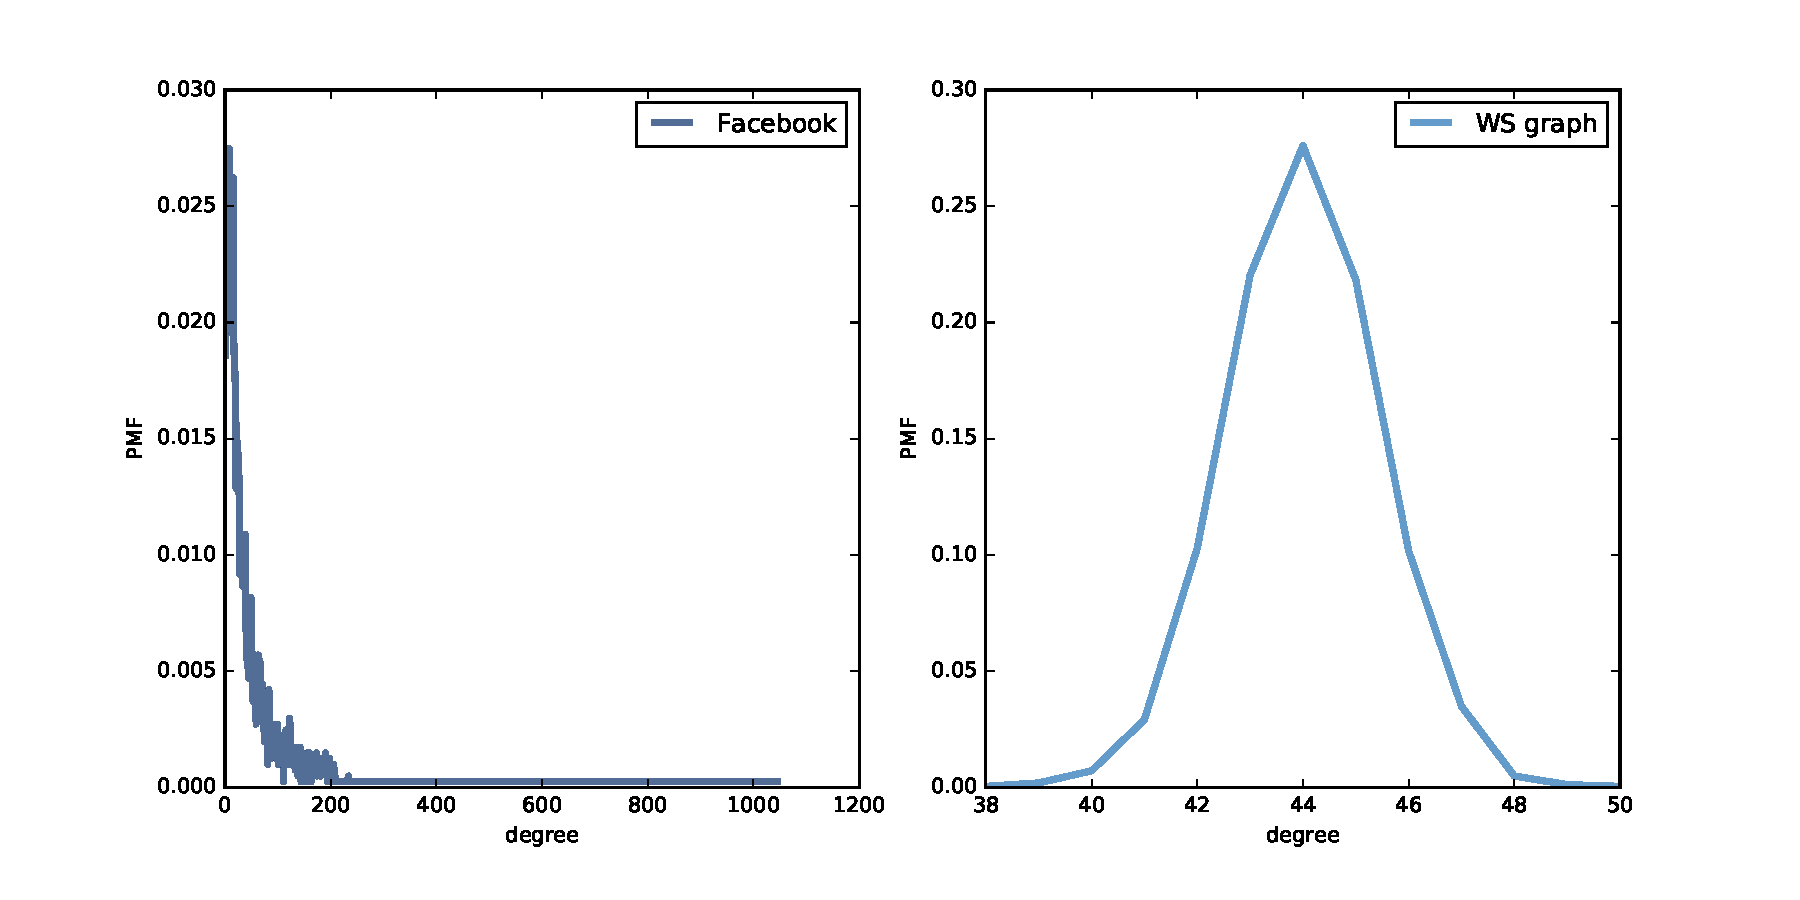
\includegraphics[width=5.5in]{figs/chap04-1.pdf}}
\caption{PMF of degree in the Facebook dataset and in the WS model.}
\label{chap04-1}
\end{figure}

Recall that the degree of a node is the number of neighbors it is
connected to.  If the WS graph is a good model for the Facebook network,
it should have the same total (or average) degree, and ideally the
same variance in degree, across nodes.

This function returns a list of degrees in a graph, one for each node:

\begin{code}
def degrees(G):
    return [G.degree(u) for u in G]
\end{code}

The mean degree in the dataset is 43.7; the mean degree in
the WS model is 44.  So far, so good.

However, the standard deviation of degrees in the WS model is 1.5;
the standard deviation in the data is 52.4.  Oops.

What's going on here?  To get a better view, we have to look at the
{\bf distribution} of degrees, not just the mean and standard deviation.

I'll represent the distribution of degrees with a \py{Pmf} object,
which is defined in the \py{thinkstats2} module.
\py{Pmf} stands for ``probability mass function'';
if you are not familiar with this concept,
you might want to read Chapter 3 of {\it Think Stats, 2nd edition}
at \url{http://greenteapress.com/thinkstats2/html/thinkstats2004.html}.

Briefly, a \py{Pmf} maps from values to their probabilities.
A \py{Pmf} of degrees is a mapping from each possible degree, $d$, to the
fraction of nodes with degree $d$.

As an example, I'll construct a graph with nodes 1, 2, and 3 connected
to a central node, 0:

\begin{code}
G = nx.Graph()
G.add_edge(1, 0)
G.add_edge(2, 0)
G.add_edge(3, 0)
nx.draw(G)
\end{code}

Here's the list of degrees in this graph:

\begin{code}
>>> degrees(G)
[3, 1, 1, 1]
\end{code}

Node 0 has degree 3, the others have degree 1.  Now I can make
a \py{Pmf} that represents this degree distribution:

\begin{code}
>>> from thinkstats2 import Pmf
>>> Pmf(degrees(G))
Pmf({1: 0.75, 3: 0.25})
\end{code}

The result is a \py{Pmf} object that maps from each degree to a
fraction or probability.  In this example, 75\% of the nodes have
degree 1 and 25\% have degree 3.

Now we can make a \py{Pmf} that contains node degrees from the
dataset, and compute the mean and standard deviation:

\begin{code}
>>> from thinkstats2 import Pmf
>>> pmf_fb = Pmf(degrees(fb))
>>> pmf_fb.Mean(), pmf_fb.Std()
(43.691, 52.414)
\end{code}

And the same for the WS model:

\begin{code}
>>> pmf_ws = Pmf(degrees(ws))
>>> pmf_ws.mean(), pmf_ws.std()
(44.000, 1.465)
\end{code}

We can use the \py{thinkplot} module to plot the results:

\begin{code}
thinkplot.Pdf(pmf_fb, label='Facebook')
thinkplot.Pdf(pmf_ws, label='WS graph')
\end{code}

Figure~\ref{chap04-1} shows the two distributions.  They are
very different.

In the WS model, most users have about 44 friends; the minimum is 38
and the maximum is 50.  That's not much variation.
In the dataset, there are many users with only 1 or 2 friends,
but one has more than 1000!

Distributions like this, with many small values and a few very large
values, are called {\bf heavy-tailed}.


\section{Heavy-tailed distributions}
\label{heavytail}

\begin{figure}
\centerline{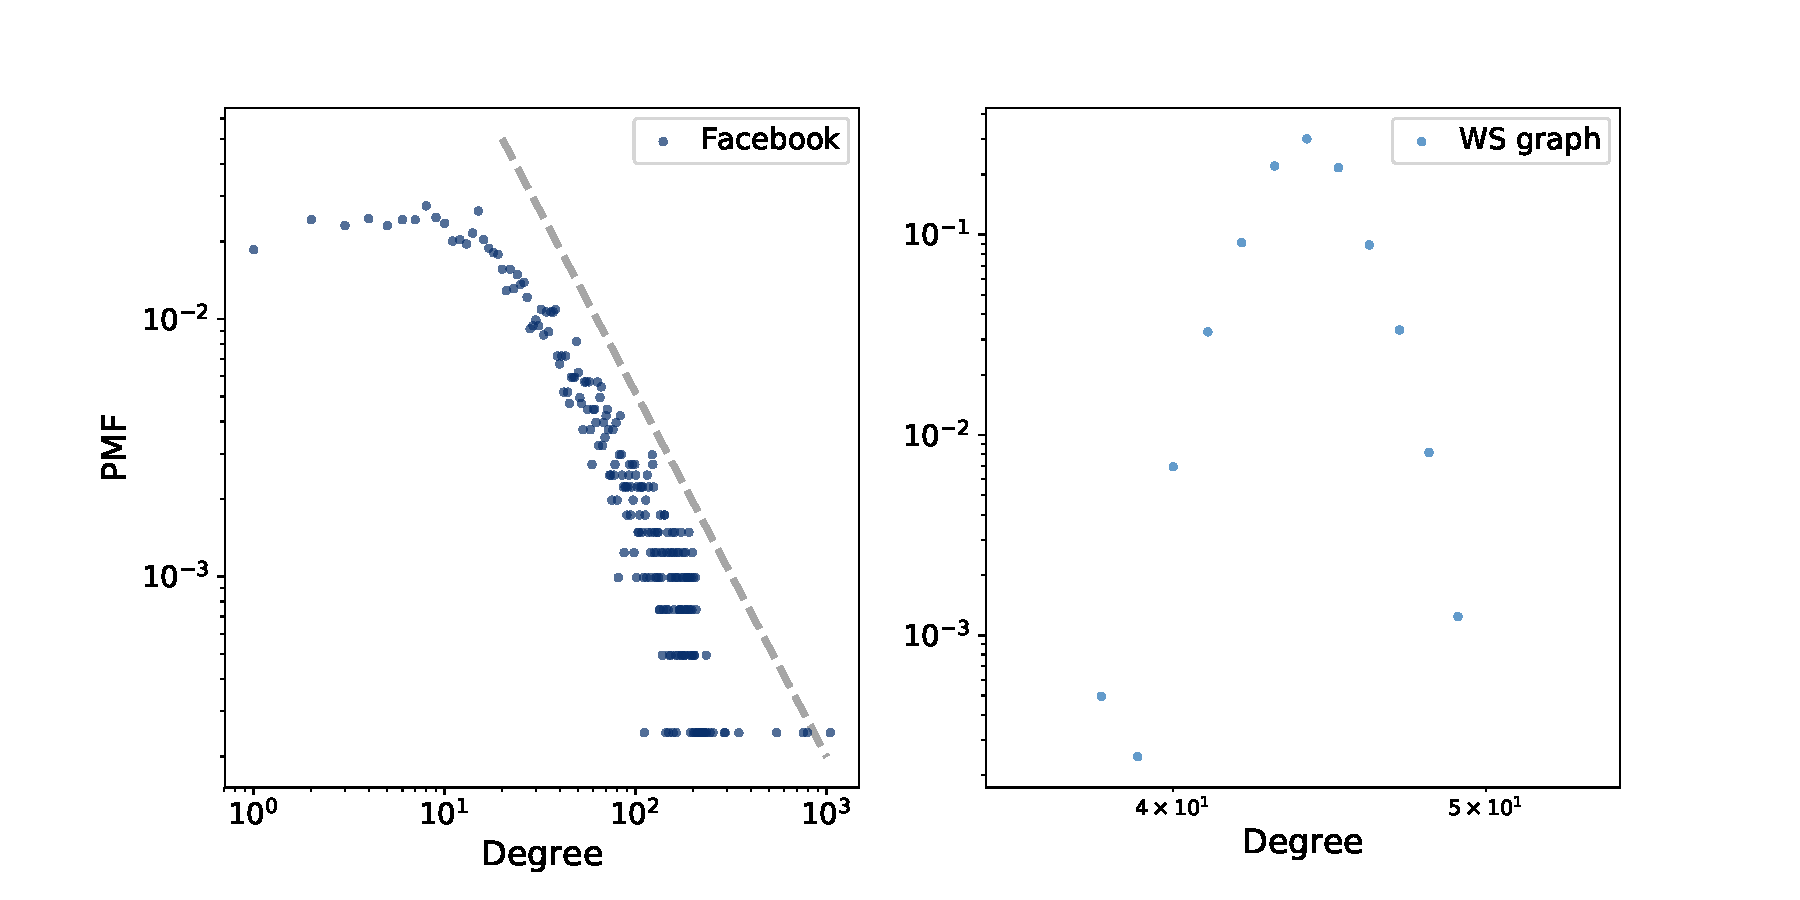
\includegraphics[width=5.5in]{figs/chap04-2.pdf}}
\caption{PMF of degree in the Facebook dataset and in the WS model,
on a log-log scale.}
\label{chap04-2}
\end{figure}

Heavy-tailed distributions are a
common feature in many areas of complexity science and they will be a
recurring theme of this book.

We can get a clearer picture of a heavy-tailed distribution by
plotting it on a log-log axis, as shown in Figure~\ref{chap04-2}.
This transformation emphasizes the tail of the distribution; that
is, the probabilities of large values.

Under this transformation, the data fall approximately on a
straight line, which suggests that there is a ``power law''
relationship between the largest values in the distribution and their
probabilities.  Mathematically,

\newcommand{\PMF}{\mathrm{PMF}}
\newcommand{\CDF}{\mathrm{CDF}}
\newcommand{\CCDF}{\mathrm{CCDF}}

\[ \PMF(k) \sim k^{-\alpha} \]

where $\PMF(k)$ is the fraction of nodes with degree $k$, $\alpha$
is a parameter, and the symbol $\sim$ indicates that the PMF is
asymptotic to $k^{-\alpha}$ as $k$ increases.

If we take the log of both sides, we get

\[ \log \PMF(k) \sim -\alpha \log k \]

So if a distribution follows a power law and we plot $\PMF(k)$ versus
$k$ on a log-log scale, we expect a straight line with slope
$-\alpha$, at least for large values of $k$.

All power law distributions are heavy-tailed, but there are other
heavy-tailed distributions that don't follow a power law.  We will
see more examples soon.

But first, we have a problem: the WS model has the high clustering
and low path length we see in the data, but the degree distribution
doesn't resemble the data at all.  This discrepancy is the motivation
for our next topic, the \Barabasi-Albert model.


\section{\Barabasi-Albert model}
\label{scale.free}

In 1999 \Barabasi~and Albert published a paper,
``Emergence of Scaling in Random Networks'', that characterizes the
structure of several real-world networks,
including graphs that represent the interconnectivity of movie actors,
world-wide web (WWW) pages, and elements in the electrical power grid
in the western United States.  You can download the paper from
\url{http://www.sciencemag.org/content/286/5439/509}.

\index{movie actor}
\index{world-wide web}
\index{electrical power grid}

They measure the degree of each node and compute $\PMF(k)$, the
probability that a vertex has degree $k$.  Then they plot $\PMF(k)$
versus $k$ on a log-log scale.  The plots fit a
straight line, at least for large values of $k$;
so \Barabasi~and Albert conclude that these
distributions are heavy-tailed.

They also propose a model that generates graphs with the same
property.  The essential features of the model, which distinguish it
from the WS model, are:
\index{generative model}

\begin{description}

\item[Growth:]  Instead of starting with a fixed number of vertices,
the BA model starts with a small graph and adds vertices one at a time.

\item[Preferential attachment:] When a new edge is created, it is
more likely to connect to a vertex that already has a large number
of edges.  This ``rich get richer'' effect is characteristic of
the growth patterns of some real-world networks.
\index{preferential attachment}
\index{rich get richer}

\end{description}

Finally, they show that graphs generated by the \Barabasi-Albert (BA)
model model have a distribution of degrees that obeys a power law.

Graphs with this property are sometimes called {\bf scale-free networks},
for reasons I won't explain; if you are curious, you can read more
at \url{http://en.wikipedia.org/wiki/Scale-free_network}.
\index{scale-free network}

NetworkX provides a function that generates BA graphs.  We will use
it first; then I'll show you how it works.

\begin{code}
ba = nx.barabasi_albert_graph(n=4039, k=22)
\end{code}

The parameters are \py{n}, the number of nodes to generate, and
\py{k}, the number of edges each node starts with when it is added to
the graph.  I chose \py{k=22} because that is the average number
of edges per node in the dataset.

\begin{figure}
\centerline{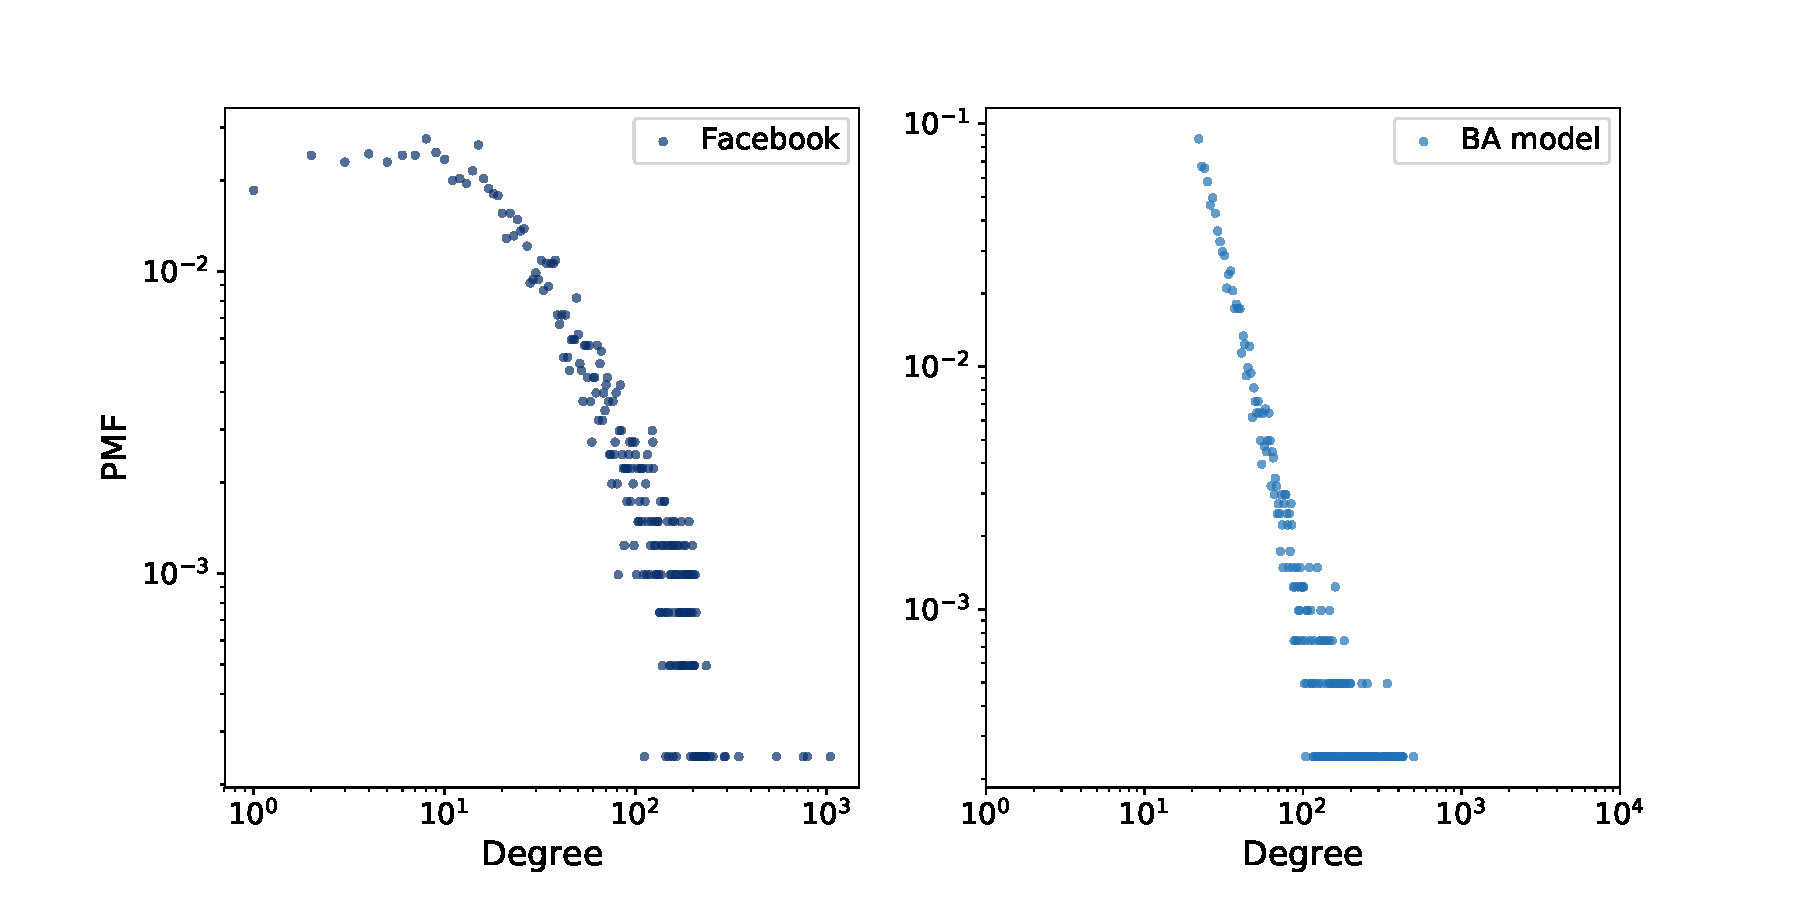
\includegraphics[width=5.5in]{figs/chap04-3.pdf}}
\caption{PMF of degree in the Facebook dataset and in the BA model,
on a log-log scale.}
\label{chap04-3}
\end{figure}

The resulting graph has 4039 nodes and 21.9 edges per node.
Since every edge is connected to two nodes, the average degree
is 43.8, very close to the average degree in the dataset,
43.7.

And the standard deviation of degree is 40.9, which is a bit
less than in the dataset, 52.4, but it is much better
than what we got from the WS graph, 1.5.

Figure~\ref{chap04-3} shows the degree distributions for the
Facebook network and the BA model on a log-log scale.  The model
is not perfect; in particular, it deviates from the data when
\py{k} is less than 10.  But the tail looks like a straight line,
which suggests that this process generates degree distributions
that follow a power law.

So the BA model is better than the WS model at reproducing the degree
distribution.  But does it have the small world property?

In this example, the average path length, $L$, is $2.5$, which
is even more ``small world'' than the actual network, which has
$L=3.69$.  So that's good, although maybe too good.

On the other hand, the clustering coefficient, $C$, is $0.037$,
not even close to the value in the dataset, $0.61$.
So that's a problem.

Table~\ref{table04-1} summarizes these results.  The WS model captures
the small world characteristics, but not the degree distribution.  The
BA model captures the degree distribution, at least approximately,
and the average path length, but not the clustering coefficient.

In the exercises at the end of this chapter, you can explore other
models intended to capture all of these characteristics.

\begin{table}[]
\centering
\begin{tabular}{lrrr}
\hline
            & \textbf{Facebook} & \textbf{WS model} & \textbf{BA model} \\
\hline
C           & 0.61             & 0.63             & 0.037             \\
L           & 3.69              & 3.23              & 2.51              \\
mean degree & 43.7              & 44                & 43.7              \\
std degree  & 52.4              & 1.5               & 40.1              \\
power law?  & maybe             & no                & yes               \\
\hline
\end{tabular}
\caption{Characteristics of the Facebook network compared to two models.}
\label{table04-1}
\end{table}


\section{Generating BA graphs}

In the previous sections we used a NetworkX function to generate BA
graphs; now let's see how it works.  Here is a version
of \py{barabasi_albert_graph}, with some changes I made to
make it easier to read:

\begin{code}
def barabasi_albert_graph(n, k):

    G = nx.empty_graph(k)
    targets = list(range(k))
    repeated_nodes = []

    for source in range(k, n):

        G.add_edges_from(zip([source]*k, targets))

        repeated_nodes.extend(targets)
        repeated_nodes.extend([source] * k)

        targets = _random_subset(repeated_nodes, k)

    return G
\end{code}

The parameters are \py{n}, the number of nodes we want, and \py{k}, the
number of edges each new node gets (which will turn out to be
approximately the number of edges per node).

We start with a graph that has \py{k} nodes and no edges.  Then we
initialize two variables:

\begin{description}

\item[\py{targets}:] The list of \py{k} nodes that will be connected
to the next node.  Initially \py{targets} contains the original
\py{k} nodes; later it will contain a random subset of nodes.

\item[\py{repeated_nodes}:] A list of existing nodes where each
node appears once for every edge it is connected to.  When we
select from \py{repeated_nodes}, the probability of selecting any
node is proportional to the number of edges it has.

\end{description}

Each time through the loop, we add edges from the source to
each node in \py{targets}.  Then we update \py{repeated_nodes} by
adding each target once and the new node \py{k} times.

Finally, we choose a subset of the nodes to be targets for the
next iteration.  Here's the definition of \py{_random_subset}:

\begin{code}
def _random_subset(repeated_nodes, k):
    targets = set()
    while len(targets) < k:
        x = random.choice(repeated_nodes)
        targets.add(x)
    return targets
\end{code}

Each time through the loop, \py{_random_subset} chooses from
\py{repeated_nodes} and adds the chosen node to \py{targets}.  Because
\py{targets} is a set, it automatically discards duplicates, so
the loop only exits when we have selected \py{k} different nodes.


\section{Cumulative distributions}
\label{cdf}

\begin{figure}
\centerline{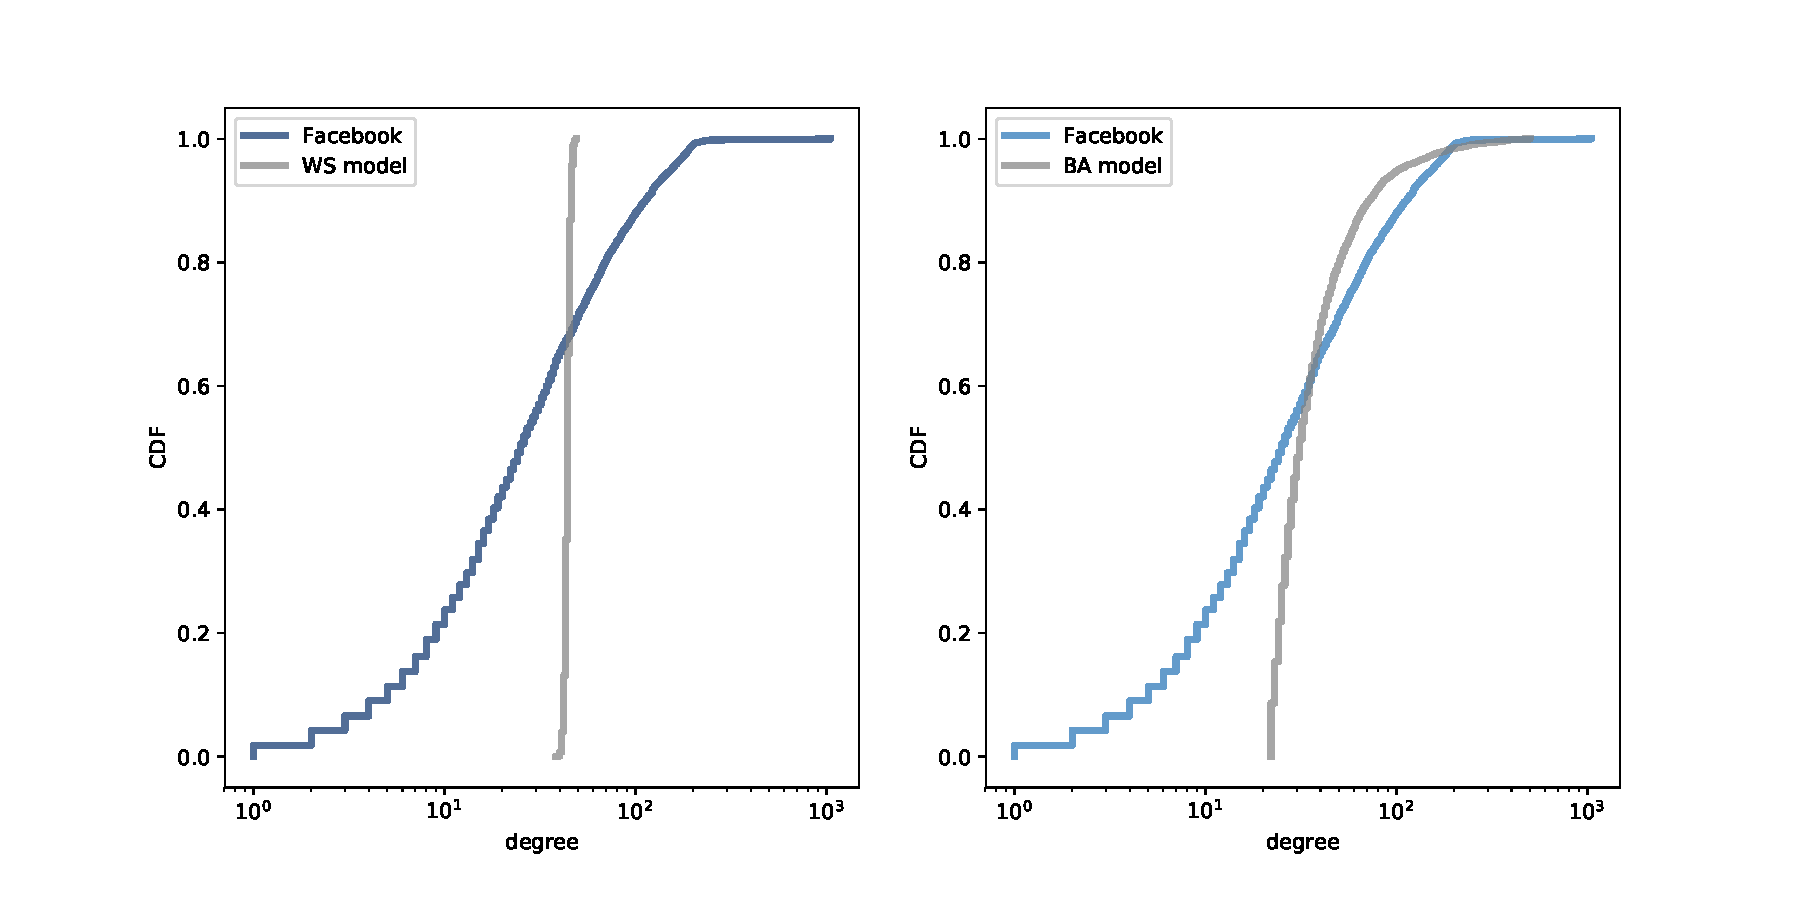
\includegraphics[width=5.5in]{figs/chap04-4.pdf}}
\caption{CDF of degree in the Facebook dataset along with the WS model (left) and the BA model (right), on a log-x scale.}
\label{chap04-4}
\end{figure}

Figure~\ref{chap04-3} represents the degree distribution by plotting
the probability mass function (PMF) on a log-log scale.  That's how
\Barabasi~and Albert present their results and it is the representation
used most often in articles about power law distributions.  But it
is not the best way to look at data like this.

A better alternative is a {\bf cumulative distribution function}
(CDF), which maps from a value, $x$, to the fraction of values less
than or equal to $x$.
\index{cumulative distribution function}
\index{CDF}

Given a \py{Pmf}, the simplest way to compute a cumulative probability
is to add up the probabilities for values up to and including $x$:

\begin{code}
def cumulative_prob(pmf, x):
    ps = [pmf[value] for value in pmf if value<=x]
    return sum(ps)
\end{code}

For example, given the degree distribution in the dataset,
\py{pmf_fb}, we can compute the fraction of users with 25 or fewer
friends:

\begin{code}
>>> cumulative_prob(pmf_fb, 25)
0.506
\end{code}

The result is close to 0.5, which means that the median number
of friends is about 25.

CDFs are better for visualization because they are less noisy than
PMFs.  Once you get used to intepreting CDFs, they provide
a clearer picture of the shape of a
distribution than PMFs.

The \py{thinkstats} module provides a class called \py{Cdf} that
represents a cumulative distribution function.  We can use it
to compute the CDF of degree in the dataset.

\begin{code}
from thinkstats2 import Cdf
cdf_fb = Cdf(degrees(fb), label='Facebook')
\end{code}

And \py{thinkplot} provides a function called \py{Cdf} that plots
cumulative distribution functions.

\begin{code}
thinkplot.Cdf(cdf_fb)
\end{code}

Figure~\ref{chap04-5} shows the degree CDF for the Facebook dataset
along with the WS model (left) and the BA model (right).  The x-axis
is on a log scale.

\begin{figure}
\centerline{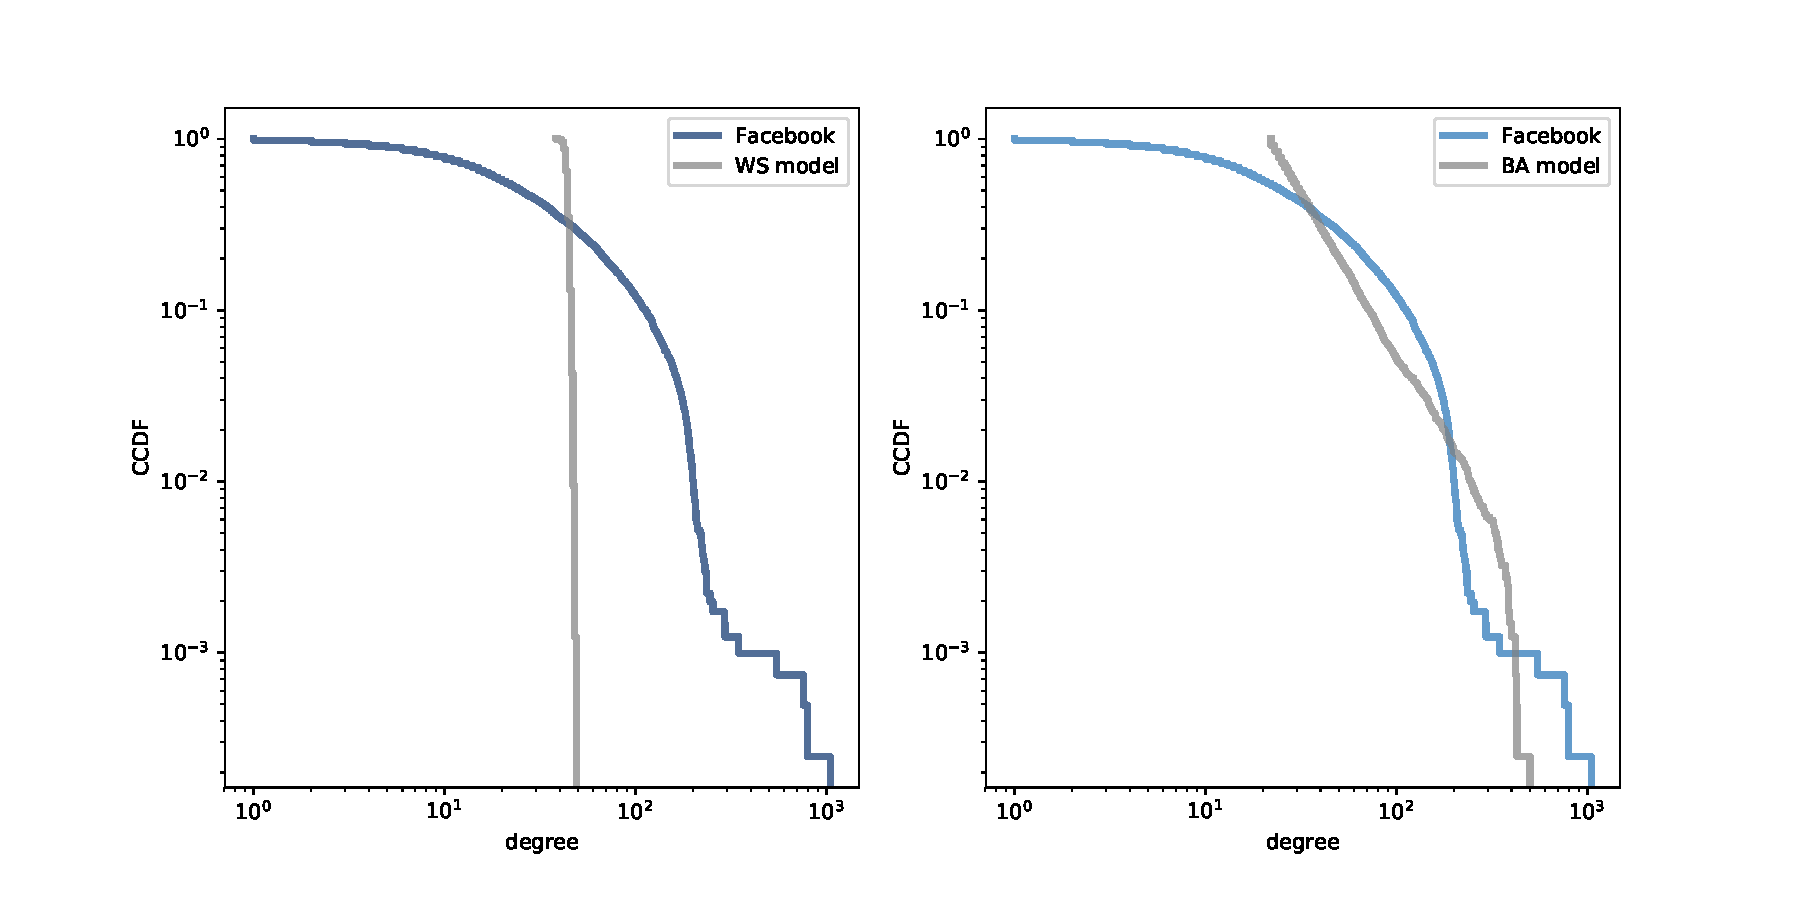
\includegraphics[width=5.5in]{figs/chap04-5.pdf}}
\caption{Complementary CDF of degree in the Facebook dataset along with the WS model (left) and the BA model (right), on a log-log scale.}
\label{chap04-5}
\end{figure}

Clearly the CDF for the WS model is very different from the CDF
from the data.  The BA model is better, but still not very good,
especially for small values.

In the tail of the distribution (values greater than 100) it looks
like the BA model matches the dataset well enough, but it is
hard to see.  We can get a clearer view with one other view of the
data: plotting the complementary CDF on a log-log scale.

The {\bf complementary CDF} (CCDF) is defined

\[ \CCDF(x) = 1 - \CDF(x) \]

If is useful because if the PMF follows a power law, the CCDF
also follows a power law:

\[ \CCDF(x) = \left( \frac{x}{x_m} \right)^{-\alpha} \]

where $x_m$ is the minimum possible value and $\alpha$ is a parameter
that determines the shape of the distribution.

Taking the log of both sides yields:

\[ \log \CCDF(x) = -\alpha (\log x - \log x_m) \]

So if the distribution obeys a power law, we expect the CCDF on
a log-log scale to be a straight line with slope $-\alpha$.

Figure~\ref{chap04-5} shows the CCDF of degree for the Facebook data,
along with the WS model (left) and the BA model (right), on a log-log
scale.

With this way of looking at the data, we can see that the BA model
matches the tail of the distribution (values above 20) reasonably well.
The WS model does not.



\section{Explanatory models}
\label{model1}

\begin{figure}
\centerline{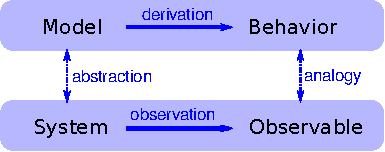
\includegraphics[height=2in]{figs/model.pdf}}
\caption{The logical structure of an explanatory model.\label{fig.model}}
\end{figure}

We started the discussion of networks with Milgram's Small World
Experiment, which shows that path lengths in social
networks are surprisingly small; hence, ``six degrees of separation''.
\index{six degrees}

When we see something surprising, it is natural to ask ``Why?''  but
sometimes it's not clear what kind of answer we are looking for.  One
kind of answer is an {\bf explanatory model} (see
Figure~\ref{fig.model}).  The logical structure of an explanatory
model is: \index{explanatory model}

\begin{enumerate}

\item In a system, S, we see something observable, O, that warrants
  explanation.
\index{system}
\index{observable}

\item We construct a model, M, that is analogous to the system; that
  is, there is a correspondence between the elements of the model and
  the elements of the system.
\index{model}

\item By simulation or mathematical derivation, we show that the model
  exhibits a behavior, B, that is analogous to O.
\index{behavior}

\item We conclude that S exhibits O {\em because} S is similar to M, M
  exhibits B, and B is similar to O.

\end{enumerate}

At its core, this is an argument by analogy, which says that if two
things are similar in some ways, they are likely to be similar in
other ways.
\index{analogy}
\index{argument by analogy}

Argument by analogy can be useful, and explanatory models can be
satisfying, but they do not constitute a proof in the mathematical
sense of the word.
\index{proof}
\index{mathematical proof}

Remember that all models leave out, or ``abstract away''
details that we think are unimportant.  For any system there
are many possible models that include or ignore different features.
And there might be models that exhibit different behaviors,
B, B' and B'', that are similar to O in different ways.
In that case, which model explains O?
\index{abstract model}

The small world phenomenon is an example: the Watts-Strogatz (WS)
model and the \Barabasi-Albert (BA) model both exhibit elements of
small world behavior, but they offer different explanations:

\begin{itemize}

\item The WS model suggests that social networks are ``small'' because
  they include both strongly-connected clusters and ``weak ties'' that
  connect clusters (see \url{http://en.wikipedia.org/wiki/Mark_Granovetter#The_strength_of_weak_ties}).
\index{weak ties}

\item The BA model suggests that social networks are small because
  they include nodes with high degree that act as hubs, and that
  hubs grow, over time, due to preferential attachment.
\index{preferential attachment}

\end{itemize}

As is often the case in young areas of science, the problem is
not that we have no explanations, but too many.


\section{Exercises}

\begin{exercise}

In Section~\ref{model1} we discussed two explanations for the
small world phenomenon, ``weak ties'' and ``hubs''.
Are these explanations compatible; that is, can they both be right?
Which do you find more satisfying as an explanation, and why?

Is there data you could collect, or experiments you could perform,
that would provide evidence in favor of one model over the other?

Choosing among competing models is the topic of Thomas Kuhn's
essay, ``Objectivity, Value Judgment, and Theory Choice'', which
you can read at
\url{https://github.com/AllenDowney/ThinkComplexity2/blob/master/papers/kuhn.pdf}.
\index{Kuhn, Thomas}
\index{theory choice}
\index{objectivity}

What criteria does Kuhn propose for choosing among competing models?
Do these criteria influence your opinion about the WS and BA models?
Are there other criteria you think should be considered?

\end{exercise}


\begin{exercise}

NetworkX provides a function called \py{powerlaw_cluster_graph} that
implements the "Holme and Kim algorithm for growing graphs with
powerlaw degree distribution and approximate average clustering".
Read the documentation of this function and see if you can use it to
generate a graph that has the same number of nodes as the Facebook
dataset, the same average degree, and the same clustering coefficient.
How does the degree distribution in the model compare to the actual
distribution?

\end{exercise}


\begin{exercise}

Data files from the \Barabasi~and Albert paper are available from
\url{http://www3.nd.edu/~networks/resources.htm}.  Their actor
collaboration data is included in the repository for this book in a
file named \py{actor.dat.gz}.  The following function reads the file and
builds the graph.

\begin{code}
import gzip

def read_actor_network(filename, n=None):
    G = nx.Graph()
    with gzip.open(filename) as f:
        for i, line in enumerate(f):
            nodes = [int(x) for x in line.split()]
            G.add_edges_from(thinkcomplexity.all_pairs(nodes))
            if n and i >= n:
                break
    return G
\end{code}

Compute the number of actors in the graph and the average degree.
Plot the PMF of degree on a log-log scale.  Also plot the CDF of
degree on a log-x scale, to see the general shape of the distribution,
and on a log-log scale, to see whether the tail follows a power law.

Note: The actor network is not connected, so you might want to use
\py{nx.connected_component_subgraphs} to find connected subsets of the
nodes.

\end{exercise}


\chapter{Cellular Automatons}
\label{automatons}

A {\bf cellular automaton} (CA) is a model of a world with very simple
physics.  ``Cellular'' means that the world is divided into discrete
chunks, called cells.  An ``automaton'' is a machine that performs
computations---it could be a real machine, but more often the
``machine'' is a mathematical abstraction or a computer simulation.
\index{cellular automaton}

This chapter presents experiments Steven Wolfram performed
in the 1980s, showing that some cellular automatons display
surprisingly complicated behavior, including the ability to
perform arbitrary computations.

I discuss implications of these results, and at the end of the
chapter I suggest methods for implementing CAs efficiently in Python.

The code for this chapter is in {\tt chap05.ipynb} in the repository
for this book.  More information about working with the code is
in Section~\ref{code}.


\section{A simple CA}

Cellular automatons\footnote{You might also see the plural
  ``automata''.} are governed by rules that determine how the system
evolves in time.  Time is divided into discrete steps, and the rules
specify how to compute the state of the world during the next time
step based on the current state.

\index{time step}

As a trivial example, consider a cellular automaton (CA) with
a single cell.  The state of the cell is an integer represented
with the variable $x_i$, where the subscript $i$ indicates
that $x_i$ is the state of the system during time step $i$.
As an initial condition, $x_0 = 0$.
\index{state}

Now all we need is a rule.  Arbitrarily, I'll pick $x_i = x_{i-1} + 1$,
which says that after each time step, the state of the CA gets
incremented by 1.  So far, we have a simple CA that performs
a simple calculation: it counts.
\index{rule}

But this CA is atypical; normally the number of
possible states is finite.  To bring it into line, I'll choose the
smallest interesting number of states, 2, and another simple rule,
$x_i = (x_{i-1} + 1) \% 2$, where $\%$ is the remainder (or
modulus) operator.

The behavior of this CA is simple: it blinks.  That is,
the state of the cell switches between 0 and 1 after every time step.

Most CAs are {\bf deterministic}, which means that rules do not
have any random elements; given the same initial state, they
always produce the same result.  There are also nondeterministic
CAs, but I will not address them here.
\index{deterministic}


\section{Wolfram's experiment}
\label{onedim}

The CA in the previous section had only one cell, so we can think of
it as zero-dimensional, and it wasn't very interesting.  In the rest
of this chapter, we explore one-dimensional (1-D) CAs, which turn out to
be surprisingly interesting.

\index{1-D cellular automaton}

To say that a CA has dimensions is to say that the cells are
arranged in a contiguous space so that some of them are
considered ``neighbors''.  In one dimension, there are three
natural configurations:
\index{neighbor}

\begin{description}

\item[Finite sequence:] A finite number of cells arranged
in a row.  All cells except the first and last have two neighbors.

\item[Ring:] A finite number of cells arranged
in a ring.  All cells have two neighbors.

\item[Infinite sequence:] An infinite number of cells arranged
in a row.

\end{description}

The rules that determine how the system evolves in time are
based on the notion of a ``neighborhood'', which is the set
of cells that determines the next state of a given cell.

In the early 1980s Stephen Wolfram published a series of papers
presenting a systematic study of 1-D CAs.  He identified
four general categories of behavior, each more interesting than
the last.

Wolfram's experiments use a 3-cell neighborhood: the cell itself
and its left and right neighbors.
\index{neighborhoos}

In these experiments, the cells have two states, denoted 0 and 1,
so the rules can be summarized by a table that maps from the
state of the neighborhood (a tuple of 3 states) to the next state
for the center cell.
The following table shows an example:
\index{rule table}
\index{state}

\centerline{
\begin{tabular}{|c|c|c|c|c|c|c|c|c|}
\hline
prev & 111 & 110 & 101 & 100 & 011 & 010 & 001 & 000 \\
\hline
next   & 0   & 0   & 1   & 1   & 0   & 0   & 1   & 0 \\
\hline
\end{tabular}}

The first row shows the eight states a
neighborhood can be in.  The second row shows the state of
the center cell during the next time step.  As a concise encoding
of this table, Wolfram suggested reading the bottom row
as a binary number.  Because 00110010 in binary is 50 in
decimal, Wolfram calls this CA ``Rule 50''.
\index{enumeration}

\begin{figure}
\centerline{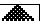
\includegraphics[height=1.5in]{figs/chap05-1.pdf}}
\caption{Rule 50 after 10 time steps.}
\label{chap05-1}
\end{figure}

Figure~\ref{chap05-1} shows the effect of Rule 50 over 10
time steps.  The first row shows the state of the system during the first
time step; it starts with one cell ``on'' and the rest ``off''.
The second row shows the state of the system during the
next time step, and so on.

The triangular shape in the figure is typical of these CAs; is it a
consequence of the shape of the neighborhood.  In one time step, each
cell influences the state of one neighbor in either direction.  During
the next time step, that influence can propagate one more cell in each
direction.  So each cell in the past has a ``triangle of influence''
that includes all of the cells that can be affected by it.
\index{triangle of influence}


\section{Classifying CAs}

\begin{figure}
\centerline{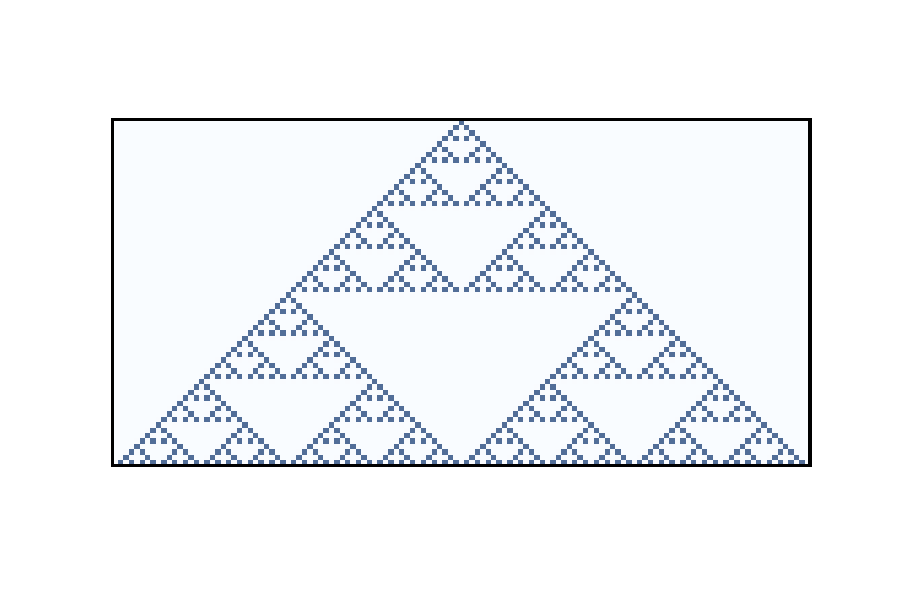
\includegraphics[height=1.5in]{figs/chap05-3.pdf}}
\caption{Rule 18 after 64 steps.}
\label{chap05-3}
\end{figure}

How many different CAs are there?

Since each cell is either on or off, we can specify the state
of a cell with a single bit.  In a neighborhood with three cells,
there are 8 possible configurations, so there are 8 entries
in the rule tables.  And since each entry contains a single bit,
we can specify a table using 8 bits.  With 8 bits, we can
specify 256 different rules.

One of Wolfram's first experiments with CA was to test all 256
possibilities and try to classify them.

Examining the results visually, he proposed that the behavior of CAs
can be grouped into four classes.  Class 1 contains the simplest (and
least interesting) CAs, the ones that evolve from almost any starting
condition to the same uniform pattern.  As a trivial example, Rule 0
always generates an empty pattern after one time step.

\index{classifying cellular automatons}

Rule 50 is an example of Class 2.  It generates a simple pattern with
nested structure; that is, the pattern contains many smaller versions
of itself.  Rule 18 makes the nested structure even clearer;
Figure~\ref{chap05-3} shows what it looks like after 64 steps.

\index{Rule 18}

\newcommand{\Sierpinski}{Sierpi\'{n}ski}

This pattern resembles the \Sierpinski~triangle, which
you can read about at \url{http://en.wikipedia.org/wiki/Sierpinski_triangle}.
\index{Sierpi\'{n}ski triangle}

Some Class 2 CAs generate patterns that are intricate and
pretty, but compared to Classes 3 and 4, they are relatively
simple.


\section{Randomness}

\begin{figure}
\centerline{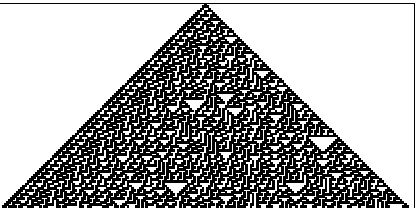
\includegraphics[height=2.5in]{figs/chap05-4.pdf}}
\caption{Rule 30 after 100 time steps.}
\label{chap05-4}
\end{figure}

Class 3 contains CAs that generate randomness.
Rule 30 is an example; Figure~\ref{chap05-4} shows what it looks like
after 100 time steps.
\index{randomness}
\index{Class 3 behavior}
\index{Rule 30}

Along the left side there is an apparent pattern, and on the right
side there are triangles in various sizes, but the center seems
quite random.  In fact, if you take the center column and treat it as a
sequence of bits, it is hard to distinguish from a truly random
sequence.  It passes many of the statistical tests people use
to test whether a sequence of bits is random.

Programs that produce random-seeming numbers are called
{\bf pseudo-random number generators} (PRNGs).  They are not considered
truly random because:

\index{pseudo-random number generator}
\index{PRNG}

\begin{itemize}

\item Many of them produce sequences with regularities that can be
  detected statistically.  For example, the original implementation of
  \py{rand} in the C library used a linear congruential generator that
  yielded sequences with easily detectable serial correlations.

  \index{linear congruential generator}

\item Any PRNG that uses a finite amount of state (that is, storage)
  will eventually repeat itself.  One of the characteristics of a
  generator is the {\bf period} of this repetition.

\index{period}

\item The underlying process is fundamentally deterministic, unlike
  some physical processes, like radioactive decay and thermal noise,
  that are considered to be fundamentally random.

\index{deterministic}

\end{itemize}

Modern PRNGs produce sequences that are statistically
indistinguishable from random, and they can be implemented with with
periods so long that the universe will collapse before they repeat.
The existence of these generators raises the question of whether there
is any real difference between a good quality pseudo-random sequence
and a sequence generated by a ``truly'' random process.  In {\em A New
  Kind of Science}, Wolfram argues that there is not (pages 315--326).
\index{New Kind of Science@{\it A New Kind of Science}}


\section{Determinism}
\label{determinism}

The existence of Class 3 CAs is surprising.  To explain how
surprising, let me start with philosophical
{\bf determinism} (see \url{http://en.wikipedia.org/wiki/Determinism}).
Many philosophical stances are hard to define precisely because
they come in a variety of flavors.  I often find it useful
to define them with a list of statements ordered from weak
to strong:
\index{determinism}

\begin{description}

\item[D1:] Deterministic models can make accurate predictions
for some physical systems.

\item[D2:] Many physical systems can be modeled by deterministic
processes, but some are intrinsically random.

\item[D3:] All events are caused by prior events, but many
physical systems are nevertheless fundamentally unpredictable.

\item[D4:] All events are caused by prior events, and can (at
least in principle) be predicted.

\index{causation}

\end{description}

My goal in constructing this range is to make D1 so weak that
virtually everyone would accept it, D4 so strong that almost no one
would accept it, with intermediate statements that some people accept.

The center of mass of world opinion swings along this range in
response to historical developments and scientific discoveries.  Prior
to the scientific revolution, many people regarded the working of the
universe as fundamentally unpredictable or controlled by supernatural
forces.  After the triumphs of Newtonian mechanics, some optimists
came to believe something like D4; for example, in 1814 Pierre-Simon
Laplace wrote

\index{Newtonian mechanics}
\index{Laplace, Pierre-Simon}

\begin{quote}
We may regard the present state of the universe as the effect of its
past and the cause of its future. An intellect which at a certain
moment would know all forces that set nature in motion, and all
positions of all items of which nature is composed, if this intellect
were also vast enough to submit these data to analysis, it would
embrace in a single formula the movements of the greatest bodies of
the universe and those of the tiniest atom; for such an intellect
nothing would be uncertain and the future just like the past would be
present before its eyes.
\end{quote}

This ``intellect'' came to be called ``Laplace's Demon''.
See \url{http://en.wikipedia.org/wiki/Laplace's_demon}.  The word
``demon'' in this context has the sense of ``spirit'', with no
implication of evil.

\index{Laplace's Demon}

Discoveries in the 19th and 20th centuries gradually dismantled
Laplace's hope.  Thermodynamics, radioactivity,
and quantum mechanics posed successive challenges to strong
forms of determinism.

\index{entropy}
\index{radioactive decay}
\index{quantum mechanics}

In the 1960s chaos theory showed that in some deterministic systems
prediction is only possible over short time scales,  limited by
precision in the measurement of initial conditions.
\index{chaos}

Most of these systems are continuous in space (if not time) and
nonlinear, so the complexity of their behavior is not entirely
surprising.  Wolfram's demonstration of complex behavior in simple
cellular automatons is more surprising---and disturbing, at least to a
deterministic world view.

\index{complex behavior}
\index{simple rules}

So far I have focused on scientific challenges to determinism, but the
longest-standing objection is the conflict between
determinism and human free will.  Complexity science provides
a possible resolution of this apparent conflict; I'll come
back to this topic in Section~\ref{freewill}.

\index{free will}


\section{Spaceships}
\label{spaceships}

\begin{figure}
\centerline{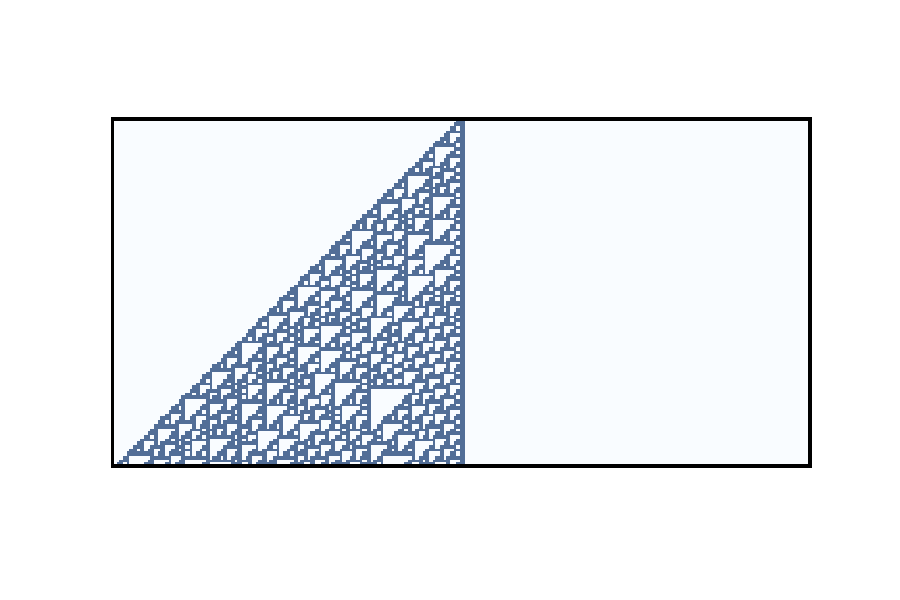
\includegraphics[height=2.5in]{figs/chap05-5.pdf}}
\caption{Rule 110 after 100 time steps.}
\label{chap05-5}
\end{figure}

The behavior of Class 4 CAs is even more surprising.  Several 1-D CAs,
most notably Rule 110, are {\bf Turing complete}, which means that
they can compute any computable function.  This property, also called
{\bf universality}, was proved by Matthew Cook in 1998.  See
\url{http://en.wikipedia.org/wiki/Rule_110}.

\index{Turing complete}
\index{universality}
\index{Cook, Matthew}

Figure~\ref{chap05-5} shows what Rule 110 looks like with an initial
condition of a single cell and 100 time steps.
At this time scale it is not apparent that anything special is
going on.  There are some regular patterns but also some features
that are hard to characterize.
\index{Rule 110}

Figure~\ref{chap05-6} shows a bigger picture, starting with a random
initial condition and 600 time steps:

\begin{figure}
\centerline{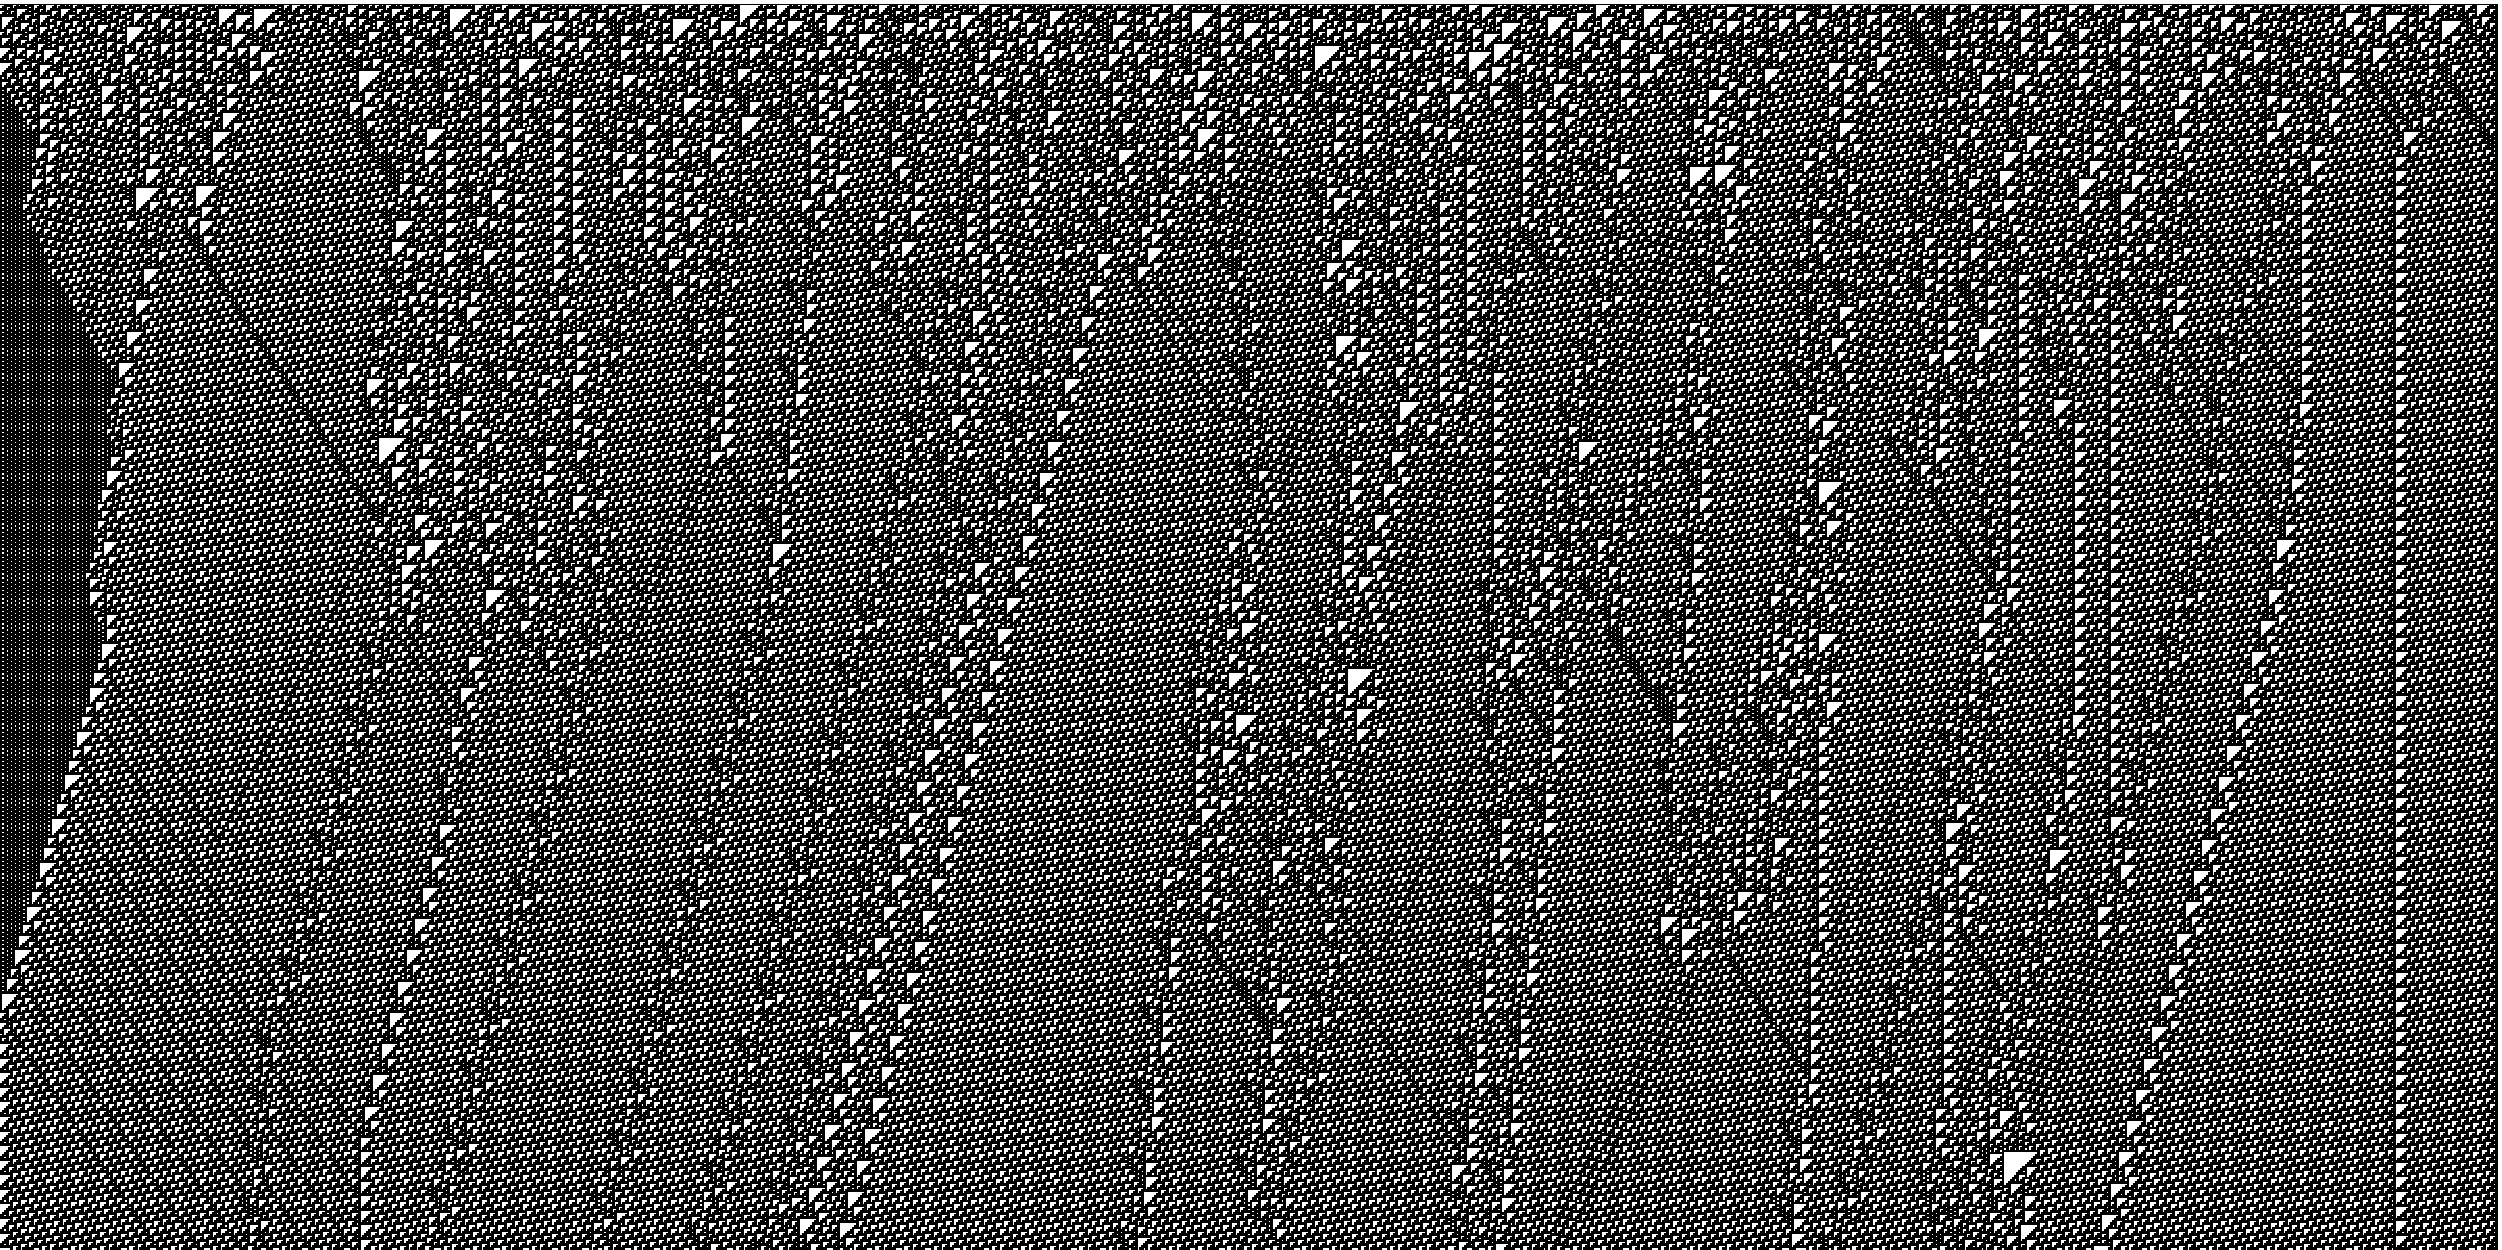
\includegraphics[width=5.5in,height=5.5in]{figs/chap05-6.pdf}}
\caption{Rule 110 with random initial conditions and 600 time steps.}
\label{chap05-6}
\end{figure}

After about 100 steps the background settles into a simple repeating
pattern, but there are a number of persistent structures that appear
as disturbances in the background.  Some of these structures
are stable, so they appear as vertical lines.  Others translate in
space, appearing as diagonals with different slopes, depending on
how many time steps they take to shift by one column.  These
structures are called {\bf spaceships}.

\index{spaceships}

Collisions between spaceships yield different results
depending on the types of the spaceships and the phase they are in
when they collide.  Some collisions annihilate both ships; others
leave one ship unchanged; still others yield one or more ships of
different types.

These collisions are the basis of computation in a Rule 110 CA.  If
you think of spaceships as signals that propagate on wires, and
collisions as gates that compute logical operations like AND and OR,
you can see what it means for a CA to perform a computation.


\section{Universality}

To understand universality, we have to understand computability
theory, which is about models of computation and what they compute.

\index{universality}

One of the most general models of computation is the Turing machine,
which is an abstract computer proposed by Alan Turing in 1936.  A
Turing machine is a 1-D CA, infinite in both directions, augmented
with a read-write head.  At any time, the head is positioned over a
single cell.  It can read the state of that cell (usually there are
only two states) and it can write a new value into the cell.

\index{Turing machine}
\index{Turing, Alan}

In addition, the machine has a register, which records the state
of the machine (one of a finite number of states), and a table
of rules.  For each machine state and cell state, the table
specifies an action.  Actions include modifying the cell
the head is over and moving one cell to the left or right.
\index{register}
\index{tape}
\index{read/write head}
\index{cell}

A Turing machine is not a practical design for a computer, but it
models common computer architectures.  For a given program running on
a real computer, it is possible (at least in principle) to construct a
Turing machine that performs an equivalent computation.

The Turing machine is useful because it is possible to characterize
the set of functions that can be computed by a Turing machine,
which is what Turing did.  Functions in this set are
called Turing computable.

\index{computable function}

To say that a Turing machine can compute any Turing-computable
function is a {\bf tautology}: it is true by definition.  But
Turing-computability is more interesting than that.

\index{tautology}

It turns out that just about every reasonable model of computation
anyone has come up with is Turing complete; that is, it can compute
exactly the same set of functions as the Turing machine.
Some of these models, like lamdba calculus, are very different
from a Turing machine, so their equivalence is surprising.

\index{lambda calculus}
\index{Church-Turing thesis}

This observation led to the Church-Turing Thesis, which is essentially
a definition of what it means to be computable.  The ``thesis'' is
that Turing-computability is the right, or at least natural,
definition of computability, because it describes the power of such a
diverse collection of models of computation.

The Rule 110 CA is yet another model of computation, and remarkable
for its simplicity.  That it, too, turns out to be universal lends
support to the Church-Turing Thesis.

In {\em A New Kind of Science}, Wolfram states a variation of this
thesis, which he calls the ``principle of computational equivalence:''

\index{principle of computational equivalence}
\index{New Kind of Science@{\it A New Kind of Science}}

\begin{quote}
Almost all processes that are not obviously simple can be viewed as
computations of equivalent sophistication.

More specifically, the principle of computational equivalence says
that systems found in the natural world can perform computations up to
a maximal (``universal'') level of computational power, and that most
systems do in fact attain this maximal level of computational
power. Consequently, most systems are computationally
equivalent (see
  \url{mathworld.wolfram.com/PrincipleofComputationalEquivalence.html}).
\end{quote}

Applying these definitions to CAs, Classes 1 and 2 are ``obviously
simple''.  It may be less obvious that Class 3 is simple, but in a way
perfect randomness is as simple as perfect order; complexity happens
in between.  So Wolfram's claim is that Class 4 behavior is common in
the natural world, and that almost all of the systems that manifest it
are computationally equivalent.
\index{Class 4 behavior}


\section{Falsifiability}

Wolfram holds that his principle is a stronger claim than the
Church-Turing Thesis because it is about the natural world rather
than abstract models of computation.  But saying that natural processes
``can be viewed as computations'' strikes me as a statement about
theory choice more than a hypothesis about the natural world.

\index{falsifiability}

Also, with qualifications like
``almost'' and undefined terms like ``obviously simple'', his
hypothesis may be {\bf unfalsifiable}.  Falsifiability is
an idea from the philosophy of science, proposed by Karl Popper
as a demarcation between scientific hypotheses and pseudoscience.
A hypothesis is falsifiable if there is an experiment, at least
in the realm of practicality, that would contradict the hypothesis
if it were false.

\index{Popper, Karl}

For example, the claim that all life on earth is descended
from a common ancestor is falsifiable because it makes specific
predictions about similarities in the genetics of modern species
(among other things).  If we discovered a new species whose
DNA was almost entirely different from ours, that would
contradict (or at least bring into question) the theory of
universal common descent.

\index{universal common descent}

On the other hand, ``special creation'', the claim that all species
were created in their current form by a supernatural agent, is
unfalsifiable because there is nothing that we could observe about the
natural world that would contradict it.  Any outcome of any experiment
could be attributed to the will of the creator.

\index{special creation}

Unfalsifiable hypotheses can be appealing because
they are impossible to refute.  If your goal is never to be
proved wrong, you should choose hypotheses that are as
unfalsifiable as possible.

But if your goal is to make reliable predictions about the world---and
this is at least one of the goals of science---unfalsifiable
hypotheses are useless.  The problem is that they have
no consequences (if they had consequences, they would be
falsifiable).

\index{prediction}

For example, if the theory of special creation were true, what good
would it do me to know it?  It wouldn't tell me anything about the
creator except that he has an ``inordinate fondness for beetles''
(attributed to J.~B.~S.~Haldane).  And unlike the
theory of common descent, which informs many areas of science
and bioengineering, it would be of no use for understanding
the world or acting in it.

\index{Haldane, J.~B.~S.}
\index{beetles}


\section{What is this a model of?}
\label{model3}

\begin{figure}
\centerline{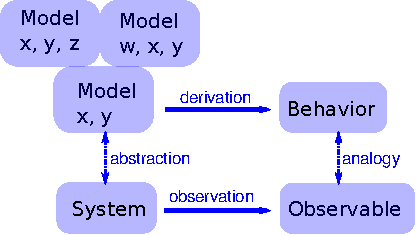
\includegraphics[height=2.5in]{figs/model3.pdf}}
\caption{The logical structure of a simple physical model.}
\label{fig.model3}
\end{figure}

Some cellular automatons are primarily mathematical artifacts.  They are
interesting because they are surprising, or useful, or pretty, or
because they provide tools for creating new mathematics (like the
Church-Turing thesis).

\index{mathematics}

But it is not clear that they are models of physical systems.  And if
they are, they are highly abstracted, which is to say that they are
not very detailed or realistic.

\index{physical model}

For example, some species of cone snail produce a pattern on their
shells that resembles the patterns generated by cellular automatons
(see \url{en.wikipedia.org/wiki/Cone_snail}).  So it is natural to
suppose that a CA is a model of the mechanism that produces patterns
on shells as they grow.  But, at least initially, it is not clear how
the elements of the model (so-called cells, communication between
neighbors, rules) correspond to the elements of a growing snail (real
cells, chemical signals, protein interaction networks).

\index{cone snail}
\index{abstract model}

For conventional physical models, being realistic is a virtue.  If the elements of a model correspond to the elements of a physical system, there is an obvious analogy between the
model and the system.  In general, we expect a model that is more
realistic to make better predictions and to provide more believable
explanations.

\index{realistic model}

Of course, this is only true up to a point.  Models that are
more detailed are harder to work with, and usually less
amenable to analysis.  At some point, a model becomes so complex
that it is easier to experiment with the system.

At the other extreme, simple models can be compelling exactly because
they are simple.

Simple models offer a different kind of explanation than detailed
models.  With a detailed model, the argument goes something
like this: ``We are interested in physical system S, so we
construct a detailed model, M, and show by analysis and simulation
that M exhibits a behavior, B, that is similar (qualitatively
or quantitatively) to an observation of the real system, O.
So why does O happen?  Because S is similar to M, and
B is similar to O, and we can prove that M leads to B.''
\index{argument by analogy}

With simple models we can't claim that S is similar to M, because it
isn't.  Instead, the argument goes like this: ``There is a set of models
that share a common set of features.  Any model that has these
features exhibits behavior B.  If we make an observation, O, that
resembles B, one way to explain it is to show that the system, S, has
the set of features sufficient to produce B.''

For this kind of argument, adding more features doesn't help.  Making
the model more realistic doesn't make the model more reliable; it only
obscures the difference between the essential features that cause O
and the incidental features that are particular to S.

Figure~\ref{fig.model3} shows the logical structure of this kind of
model.  The features $x$ and $y$ are sufficient to produce the
behavior.  Adding more detail, like features $w$ and $z$, might make
the model more realistic, but that realism adds no explanatory power.


\section{Implementing CAs}

\begin{figure}
\centerline{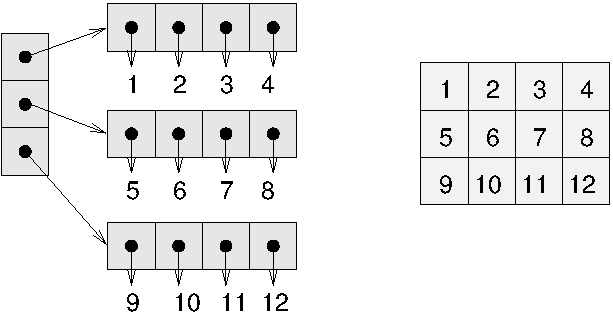
\includegraphics[height=1.75in]{figs/array.pdf}}
\caption{A list of lists (left) and a Numpy array (right).\label{fig.array}}
\end{figure}

To generate the figures in this chapter, I wrote a Python class called
\py{CA}, which represents a cellular automaton, and classes for plotting
the results.  In the next few sections I explain how they work.

\index{implementing cellular automatons}

To store the state of the CA, I use a NumPy array, which is a
multi-dimensional data structure whose elements are all the same type.
It is similar to a nested list, but usually smaller and faster.
Figure~\ref{fig.array} shows why.
The diagram on the left shows a list of lists of integers; each
dot represents a reference, which takes up 4--8 bytes.  To access
one of the integers, you have to follow two references.
\index{NumPy}
\index{array}
\index{nested list}
\index{reference}

The diagram on the right shows an array of the same integers.  Because
the elements are all the same size, they can be stored contiguously in
memory.  This arrangement saves space because it doesn't use
references, and it saves time because the location of an element can
be computed directly from the indices; there is no need to follow a
series of references.

To explain how my code works, I'll start with a CA that computes the
``parity'' of the cells in each neighborhood.  The parity of a number
is 0 if the number is even and 1 if it is odd.

First I create an array of zeros with a single 1 in the middle of
the first row.

\begin{code}
>>> rows = 5
>>> cols = 11
>>> ca = np.zeros((rows, cols))
>>> ca[0, 5] = 1
print(ca)
[[ 0.  0.  0.  0.  0.  1.  0.  0.  0.  0.  0.]
 [ 0.  0.  0.  0.  0.  0.  0.  0.  0.  0.  0.]
 [ 0.  0.  0.  0.  0.  0.  0.  0.  0.  0.  0.]
 [ 0.  0.  0.  0.  0.  0.  0.  0.  0.  0.  0.]
 [ 0.  0.  0.  0.  0.  0.  0.  0.  0.  0.  0.]]
\end{code}

\py{plot_ca} displays the results graphically:

\begin{code}
import matplotlib.pyplot as plt

def plot_ca(ca, rows, cols):
    cmap = plt.get_cmap('Blues')
    plt.imshow(array, interpolation='none', cmap=cmap)
\end{code}

Following convention, I import \py{pyplot} with the abbreviated name
\py{plt}.  \py{imshow} treats the array as an ``image'' and displays
it.  Using the colormap \py{'Blues'} draws the on cells in dark blue and
the off cells in light blue.

Now, to compute the state of the CA during the next time step,
we can use \py{step}:

\begin{code}
def step(array, i):
    rows, cols = array.shape
    for j in range(1, cols):
        array[i, j] = sum(array[i-1, j-1:j+2]) % 2
\end{code}

The parameter \py{ca} is the NumPy array that represents the state of
the CA.  \py{rows} and \py{cols} are the dimensions of the array, and
\py{i} is the index of the timestep we should compute.  I use \py{i} to
indicate rows of the array, which correspond to time, and \py{j} to
indicate columns, which correspond to space.

Inside \py{step} we loop through the elements of row \py{i}.  Each
element is the sum of three elements from the previous row, mod 2.


\section{Cross-correlation}
\label{cross-correlation}

The \py{step} function in the previous section is simple, but it is
not very fast.  In general, we can speed up operations like this
if we replace \py{for} loops with NumPy operations, because
\py{for} loops incur a lot of overhead in the Python interpreter.
In this section I'll show how we can speed up \py{step} using the
NumPy function \py{correlate}.

First, instead of using a slice operator to select a neighborhood,
we can use array multiplication.  Specifically,
we multiply \py{array} by a {\bf window}
that contains ones for the cells we want to select and zeros for
the rest.

For example, the following window selects the first three elements:

\begin{code}
>>> window = np.zeros(cols, dtype=np.int8)
>>> window[:3] = 1
>>> print(window)
[1 1 1 0 0 0 0 0 0 0 0]
\end{code}

If we multiply by the last row of \py{array}, we get the first
three elements:

\begin{code}
>>> print(array[4])
>>> print(window * array[4])
[0 1 0 0 0 1 0 0 0 1 0]
[0 1 0 0 0 0 0 0 0 0 0]
\end{code}

Now we can use \py{sum} and the modulus operator
to compute the first element of the next row:

\begin{code}
>>> sum(window * array[4]) % 2
1
\end{code}

If we shift the window to the right, it selects the next three
elements, and so on.  So we can rewrite \py{step} like this:

\begin{code}
def step2(array, i):
    rows, cols = array.shape
    window = np.zeros(cols)
    window[:3] = 1
    for j in range(1, cols):
        array[i, j] = sum(window * array[i-1]) % 2
        window = np.roll(window, 1)
\end{code}

\py{roll} shifts the window to the right (it also wraps it around to the
beginning, but that doesn't affect this function).

\py{step2} yields the same results as \py{step}.  It is still not
very fast, but it is a step in the right direction because the
operation we just performed---multiplying by a window, summing
the result, shifting the window, and repeating---is used for a
variety of applications.  It is called {\bf cross-correlation},
and NumPy provides
a function called \py{correlate} that computes it.

We can use it to write faster, simpler version of \py{step}:

\begin{code}
def step3(array, i):
    window = np.array([1, 1, 1])
    array[i] = np.correlate(array[i-1], window, mode='same') % 2
\end{code}

When we use
\py{np.correlate}, the window does not have to be the same size as
\py{array}, so making the window is a little simpler.

The \py{mode} parameter determines the size of the result.  You can
read the details in the NumPy documentation, but when the mode is
\py{'same'}, the result is the same size as the input.


\section{CA tables}
\label{tables}

Now there's just one more step.  The function we have so far
works if the CA rule only depends on the sum of the neighbors, but
most rules also depend on which neighbors are on and off.  For
example, \py{100} and \py{001} might yield different results.

We can make \py{step} more general using a window with elements
\py{[4, 2, 1]}, which interprets the neighborhood as a binary number.
For example, the neighborhood \py{100} yields 4; \py{010} yields 2,
and \py{001} yields 1.  Then we can take these results and look them
up in the rule table.

Here's the more general version of \py{step}:

\begin{code}
def step4(array, i):
    window = np.array([4, 2, 1])
    corr = np.correlate(array[i-1], window, mode='same')
    array[i] = table[corr]
\end{code}

The first two lines are almost the same.  The last line looks
up each element from \py{corr} in \py{table} and assigns the
results to \py{array[i]}.

Finally, here's the function that computes the table:

\begin{code}
def make_table(rule):
    rule = np.array([rule], dtype=np.uint8)
    table = np.unpackbits(rule)[::-1]
    return table
\end{code}

The parameter, \py{rule}, is an integer between 0 and 255.
The first line put the rule into an array with a single element
so we can use \py{unpackbits}, which converts the rule number
to its binary representation.  For
example, here's the table for Rule 150:

\begin{code}
>>> table = make_table(150)
>>> print(table)
[0 1 1 0 1 0 0 1]
\end{code}

In \py{thinkcomplexity.py}, you'll find definitions for \py{CA},
which encapsulates the code in this section, and two classes
that draw CAs, \py{PyplotDrawer} and \py{EPSDrawer}.


\section{Exercises}

\begin{exercise}

The code for this chapter is in the Jupyter notebook {\tt chap05.ipynb}
in the repository for this book.  Open this notebook, read the code,
and run the cells.  You can use this notebook to work on the
exercises in this chapter.  My solutions are in {\tt chap05soln.ipynb}.

\end{exercise}



\begin{exercise}

This exercise asks you to experiment with Rule 110 and
some of its spaceships.

\begin{enumerate}

\item Read the Wikipedia page about Rule 110, which describes its
  background pattern and spaceships:
  \url{https://en.wikipedia.org/wiki/Rule_110}.

\item Create a Rule 110 CA with an initial condition that yields the
  stable background pattern.

Note that the CA class provides
\py{start_string}, which allow you to initialize the state of
the array using a string of \py{1}s and \py{0}s.

\item Modify the initial condition by adding different patterns in the
  center of the row and see which ones yield spaceships.  You might
  want to enumerate all possible patterns of $n$ bits, for some
  reasonable value of $n$.  For each spaceship, can you find the
  period and rate of translation?  What is the biggest spaceship you
  can find?

\item What happens when spaceships collide?

\end{enumerate}

\end{exercise}



\begin{exercise}

The goal of this exercise is to implement a Turing machine.

\begin{enumerate}

\item Read about Turing machines at \url{http://en.wikipedia.org/wiki/Turing_machine}.

\item Write a class called \py{Turing} that implements a Turing machine.
For the action table, use the rules for a 3-state busy beaver.
\index{busy beaver}

\item Write a class named \py{TuringDrawer} that generates an
image that represents the state of the tape and the position and
state of the head.  For one example of what that might look like,
see \url{http://mathworld.wolfram.com/TuringMachine.html}.

\end{enumerate}

\end{exercise}


\begin{exercise}

This exercise asks you to implement and test several PRNGs.
For testing, you will need to install
\py{DieHarder}, which you can download from
\url{https://www.phy.duke.edu/~rgb/General/dieharder.php}, or it
might be available as a package for your operating system.
\index{DieHarder}

\begin{enumerate}

\item Write a program that implements one of the linear congruential
generators described at
\url{http://en.wikipedia.org/wiki/Linear_congruential_generator}).
Test it using \py{DieHarder}.

\item Read the documentation of Python's \py{random} module.
What PRNG does it use?  Test it.
\index{random module@\py{random} module}

\item Implement a Rule 30 CA with a few hundred cells,
run it for as many time steps as you can in a reasonable amount
of time, and output the center column as a sequence of bits.
Test it.
\index{Rule 30}

\end{enumerate}

\end{exercise}


\begin{exercise}

Falsifiability is an appealing and useful idea, but among
philosophers of science it is not generally accepted
as a solution to the demarcation problem, as Popper claimed.

Read \url{http://en.wikipedia.org/wiki/Falsifiability} and answer the
following questions.

\begin{enumerate}

\item What is the demarcation problem?
\index{demarcation problem}

\item How, according to Popper, does falsifiability solve the
demarcation problem?

\item Give an example of two theories, one considered scientific
and one considered unscientific, that are successfully distinguished
by the criterion of falsifiability.

\item Can you summarize one or more of the objections that
philosophers and historians of science have raised to Popper's
claim?

\item Do you get the sense that practicing philosophers think
highly of Popper's work?

\end{enumerate}

\end{exercise}




\chapter{Game of Life}

In this chapter we consider two-dimensional cellular automatons,
especially John Conway's Game of Life (GoL).  Like some of
the 1-D CAs in the previous chapter, GoL follows simple rules and
produces surprisingly complicated behavior.  And like Wolfram's
Rule 110, GoL turns out to be universal; that is, it can compute
any computable function, at least in theory.

Complex behavior in GoL raises issues in the philosophy of
science, particularly related to scientific realism and instrumentalism.
I discuss these issues and suggest additional reading.

At the end of the chapter, I demonstrate ways to implement
GoL efficiently in Python.

The code for this chapter is in {\tt chap06.ipynb} in the repository
for this book.  More information about working with the code is
in Section~\ref{code}.


\section{Conway's GoL}

\label{life}

One of the first cellular automatons to be studied, and probably the
most popular of all time, is a 2-D CA called ``The Game of Life'', or GoL
for short.  It was developed by John H. Conway and popularized in 1970
in Martin Gardner's column in {\em Scientific American}.
See \url{http://en.wikipedia.org/wiki/Conway_Game_of_Life}.
\index{Game of Life}
\index{Conway, John H.}
\index{Gardner, Martin}

The cells in GoL are arranged in a 2-D {\bf grid}, either infinite in
both directions or wrapped around.  A grid wrapped in both directions
is called a {\bf torus} because it is topographically equivalent to
the surface of a doughnut.  See
\url{http://en.wikipedia.org/wiki/Torus}.

\index{grid}
\index{torus}

Each cell has two states---live and dead---and 8 neighbors---north,
south, east, west, and the four diagonals.  This set of neighbors
is sometimes called a ``Moore neighborhood''.

\index{Moore neighborhood}
\index{neighborhood}

Like the 1-D CAs in the previous chapters, the Game of Life evolves
over time according to rules, which are like simple laws of physics.

In GoL, the next state of each cell depends on its current state and
its number of live neighbors.  If a cell is alive, it survives if it
has 2 or 3 neighbors and dies otherwise.  If a cell is
dead, it stays dead unless it has exactly 3 neighbors.

The following table summarizes the rules:

\begin{tabular}{|l|c|c|}
\hline
Current    &    Number of     & Next \\
state      &    neighbors     & state \\
\hline
live       &  2--3          & live         \\
live       &  0--1, 4--8    & dead         \\
dead       &  3             & live         \\
dead       &  0--2, 4--8    & dead         \\
\hline
\end{tabular}

This behavior is loosely analogous to real cell growth: cells
that are isolated or overcrowded die; at moderate densities they
flourish.

GoL is popular because:

\begin{itemize}

\item There are simple initial conditions that yield
surprisingly complex behavior.

\index{complex behavior}

\item There are many interesting stable patterns: some
oscillate (with various periods) and some move like the
spaceships in Wolfram's Rule 110 CA.

\item And like Rule 110, GoL is Turing complete.

\index{Turing complete}
\index{universal}

\item Another factor that generated interest was Conway's
conjecture---that there is
no initial condition that yields unbounded growth in the number
of live cells---and the \$50 bounty he offered to anyone who could prove
or disprove it.

\index{unbounded}

\item Finally, the increasing availability of computers made it
  possible to automate the computation and display the results
  graphically.

\end{itemize}



\section{Life patterns}
\label{lifepatterns}

\begin{figure}
\centerline{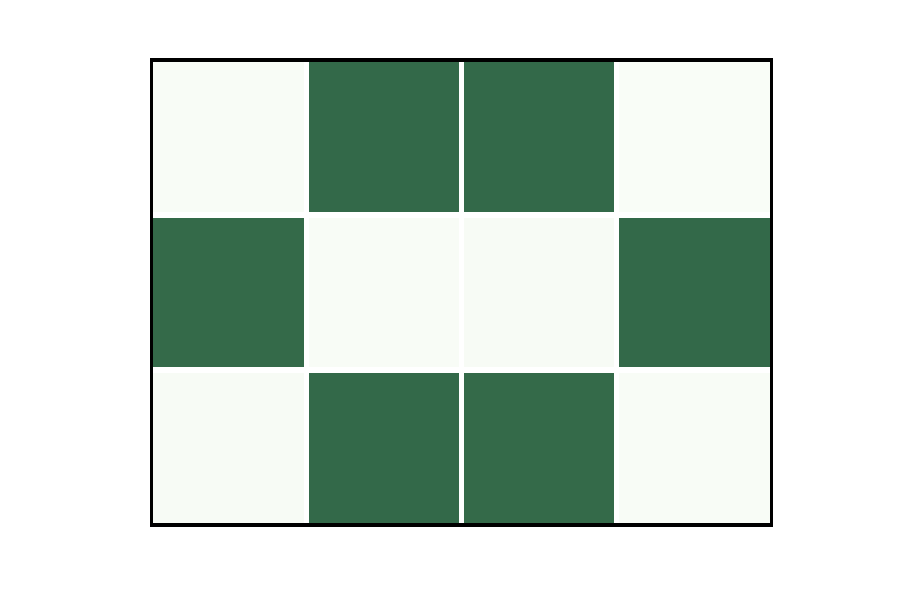
\includegraphics[height=1.75in]{figs/chap06-1.pdf}}
\caption{A stable pattern called a beehive.}
\label{chap06-1}
\end{figure}

\begin{figure}
\centerline{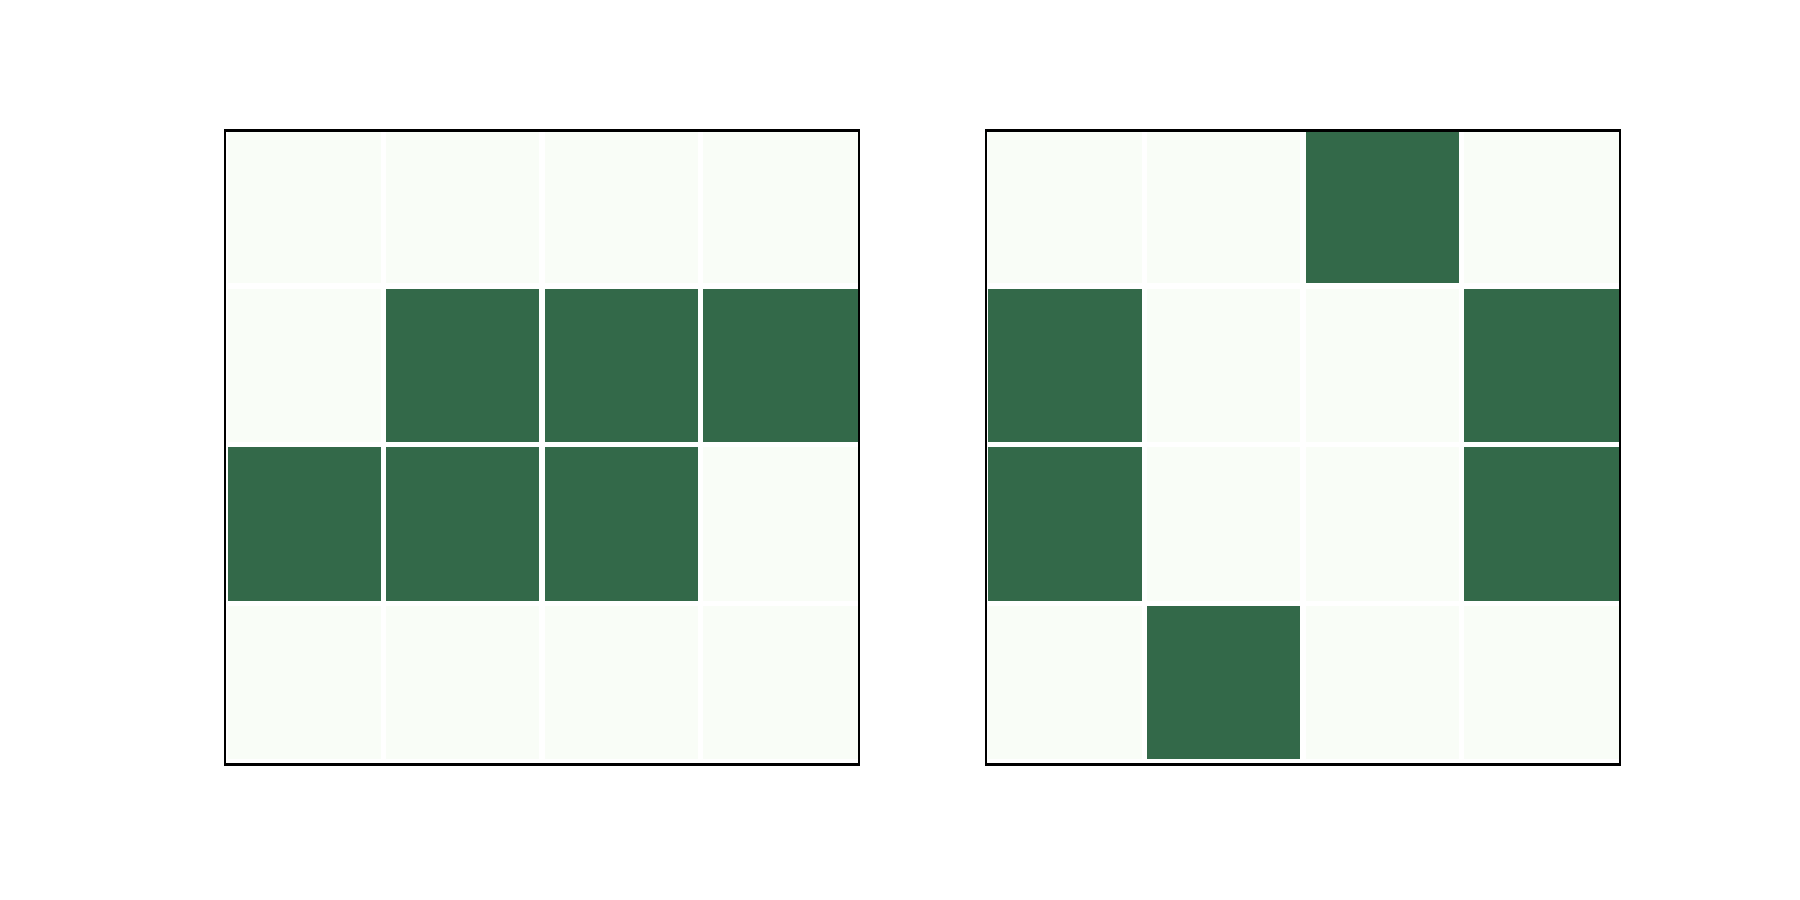
\includegraphics[height=1.75in]{figs/chap06-2.pdf}}
\caption{An oscillator called a toad.}
\label{chap06-2}
\end{figure}

\begin{figure}
\centerline{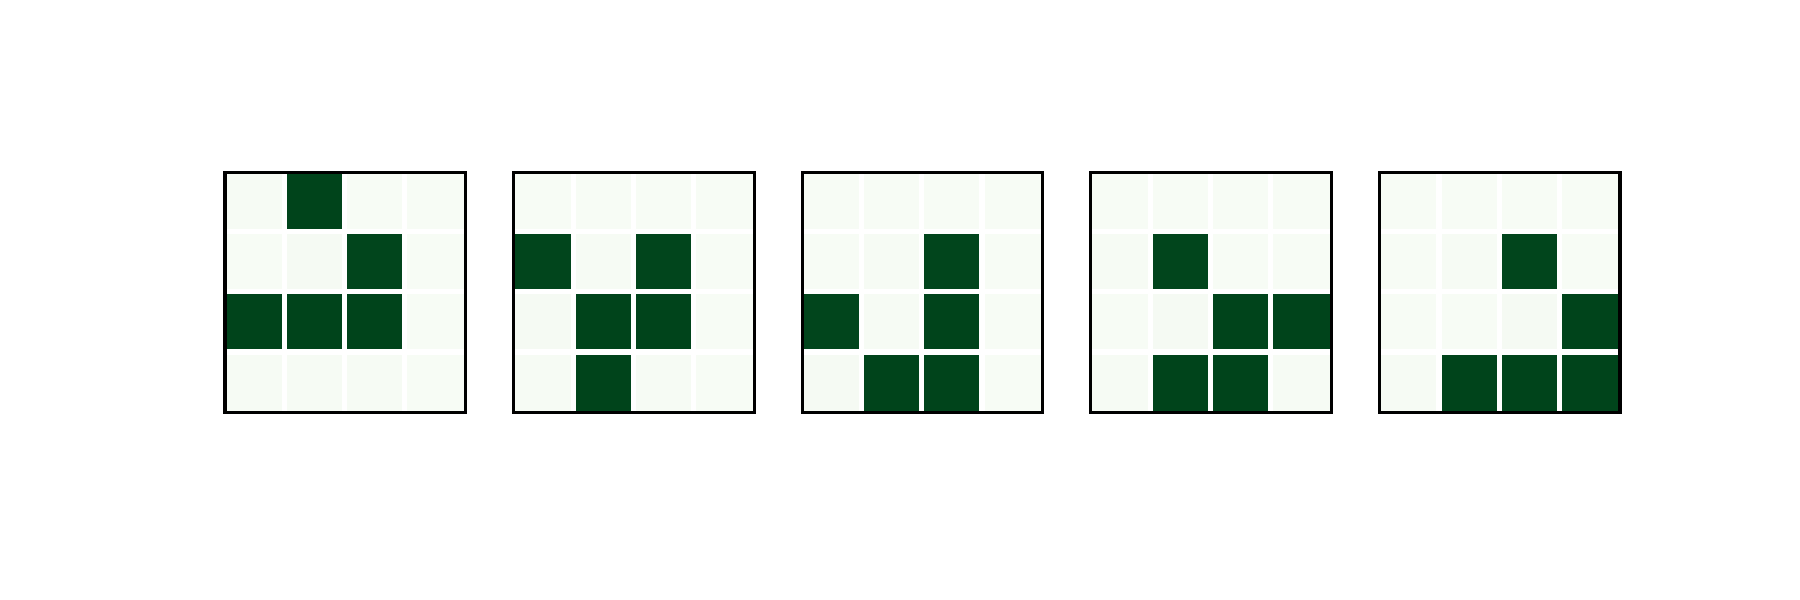
\includegraphics[height=1.75in]{figs/chap06-3.pdf}}
\caption{A spaceship called a glider.}
\label{chap06-3}
\end{figure}

If you run GoL from a random starting state, a number of stable
patterns are likely to appear.  Over time, people have identified
these patterns and given them names.

\index{Game of Life patterns}

For example, Figure~\ref{chap06-1} shows a stable pattern called a
``beehive''.  Every cell in the beehive
has 2 or 3 neighbors, so they all survive, and none of the dead
cells adjacent to the beehive has 3 neighbors, so no new cells
are born.

Other patterns ``oscillate''; that is, they change over time but
eventually return to their starting configuration (provided
they don't collide with another pattern).  For example,
Figure~\ref{chap06-2} shows a pattern called a ``toad'', which
is an oscillator that alternates between two states.  The
``period'' of this oscillator is 2.

\index{oscillator}

Finally, some patterns oscillate and return to the starting
configuration, but shifted in space.  Because these patterns
seem to move, they are called ``spaceships''.

Figure~\ref{chap06-3} shows a spaceship called a
``glider''.  After a period of 4 steps, the glider is back in the
starting configuration, shifted one unit down and to the right.

\index{glider}
\index{spaceship}

Depending on the starting orientation, gliders can move along any
of the four diagonals.  There are other spaceships that
move horizontally and vertically.

People have spent embarrassing
amounts of time finding and naming these patterns.  If you search
the web, you will find many collections.

\section{Conway's conjecture}

From most initial conditions, GoL quickly reaches a stable
state where the number of live cells is nearly constant
(possibly with some oscillation).

\begin{figure}
\centerline{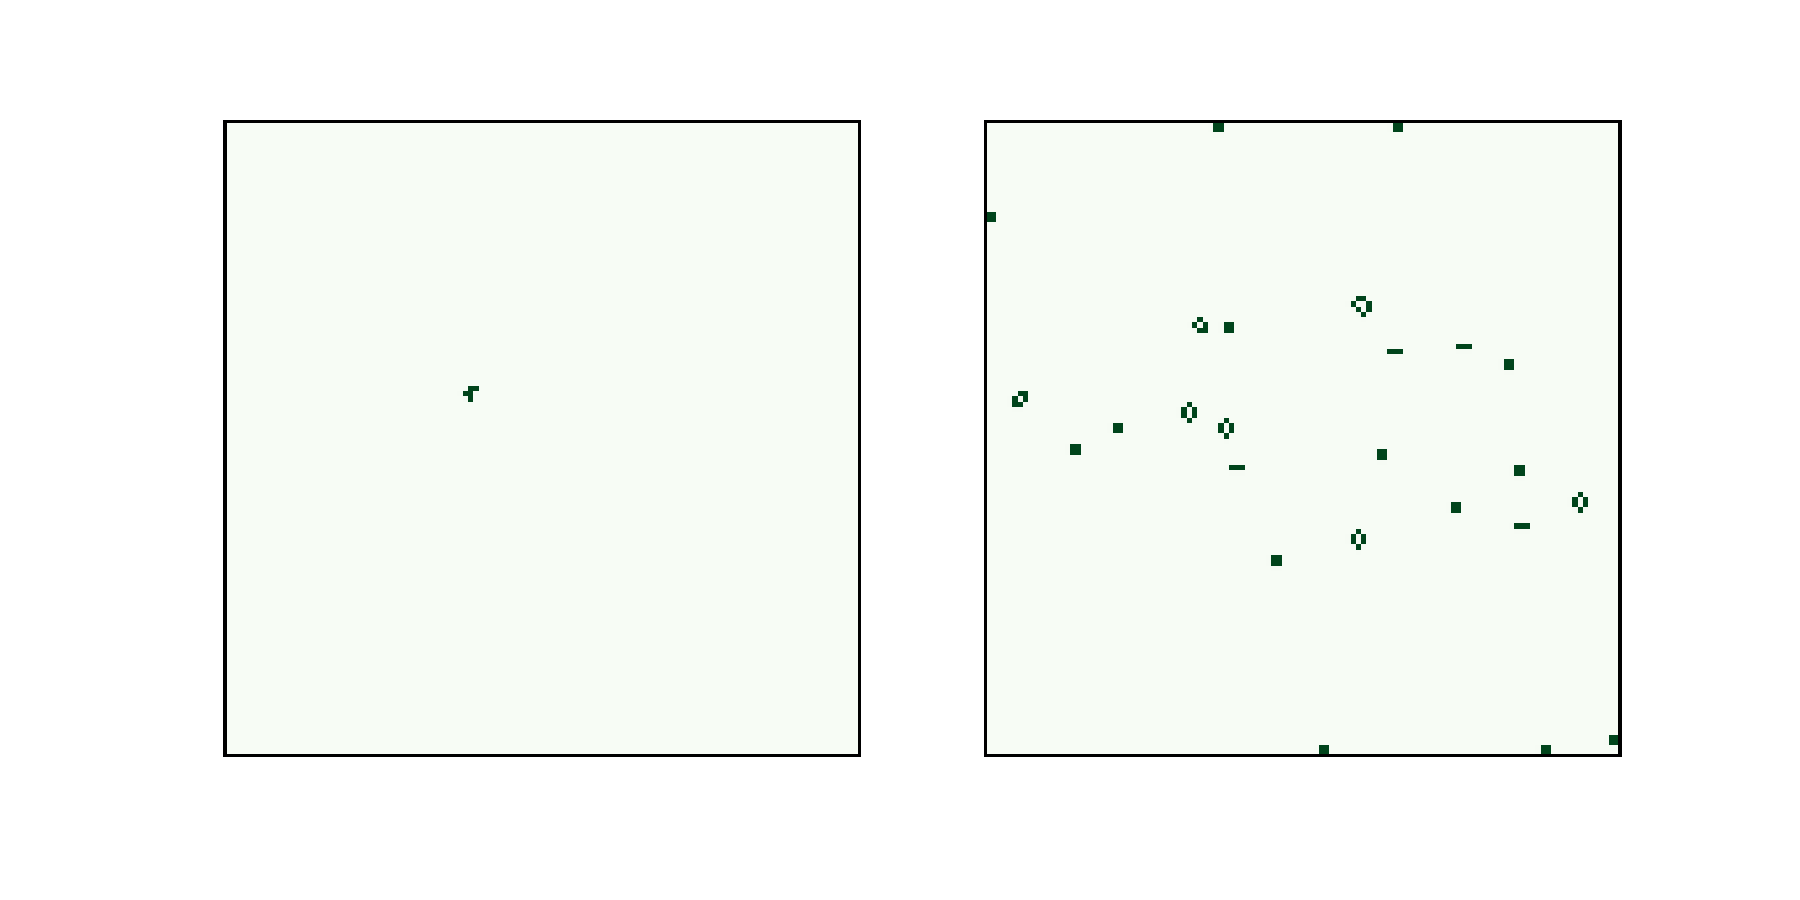
\includegraphics[height=1.75in]{figs/chap06-4.pdf}}
\caption{Starting and final configurations of the r-pentomino.}
\label{chap06-4}
\end{figure}

But there are a some simple starting conditions that take a
long time to settle down and yield a surprising
number of live cells.  These patterns are called ``Methuselahs''
because they are so long-lived.

\index{Methuselah}

One of the simplest is the
r-pentomino, which has only five cells, roughly in the shape of the
letter ``r''.  Figure~\ref{chap06-4} shows the initial configuration
of the r-pentomino and the final configuration after 1103 steps.

This configuration is ``final'' in the sense that all remaining
patterns are either stable, oscillators, or gliders that will never
collide with another pattern.  In total, the r-pentomino yields 6
gliders, 8 blocks, 4 blinkers, 4 beehives, 1 boat, 1 ship, and 1 loaf.

\index{r-pentomino}


\begin{figure}
\centerline{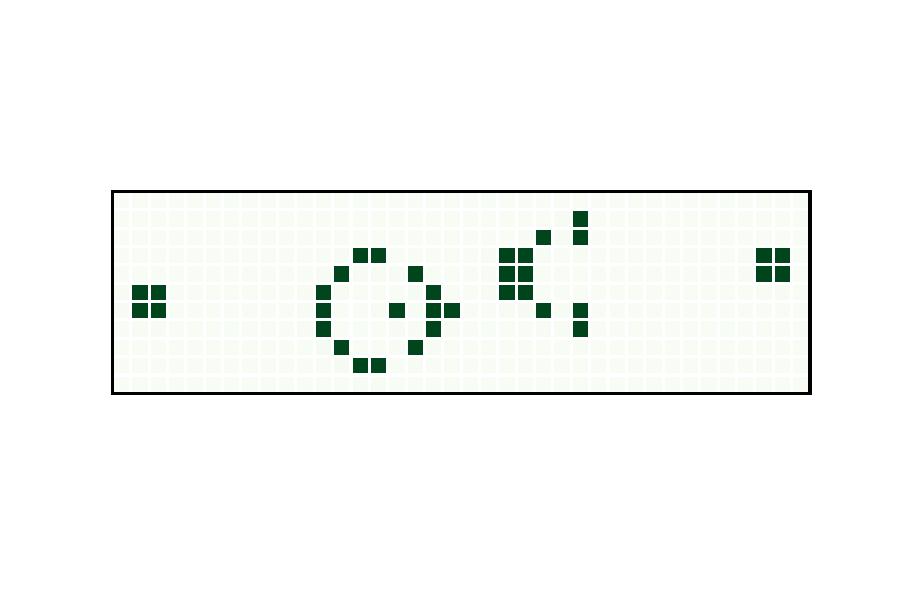
\includegraphics[height=1.75in]{figs/chap06-5.pdf}}
\caption{Gosper's glider gun, which produces a stream of gliders.}
\label{chap06-5}
\end{figure}

The existence of long-lived patterns prompted Conway to wonder if
there are initial patterns that never stabilize.  He
conjectured that there were not, but he described two kinds of pattern
that would prove him wrong, a ``gun'' and a ``puffer train''.  A gun
is a stable pattern that periodically produces a spaceship---as the
stream of spaceships moves out from the source, the number of live
cells grows indefinitely.  A puffer train is a translating pattern
that leaves live cells in its wake.

\index{glider gun}
\index{puffer train}

It turns out that both of these patterns exist.  A team led
by Bill Gosper discovered the first, a glider gun now called
Gosper's Gun, which is shown in Figure~\ref{chap06-5}.
Gosper also discovered the first puffer train.

\index{Gosper, Bill}

There are many patterns of both types, but they are not easy to
design or find.  That is not a coincidence.  Conway chose the
rules of GoL so that his conjecture would not be obviously
true or false.  Of all possible rules for a 2-D CA, most
yield simple behavior: most initial conditions stabilize quickly
or grow unboundedly.  By avoiding uninteresting CAs, Conway
was also avoiding Wolfram's Class 1 and Class 2 behavior, and
probably Class 3 as well.

If we believe Wolfram's Principle of Computational Equivalence, we
expect GoL to be in Class 4, and it is.  The Game of Life was proved
Turing complete in 1982 (and again, independently, in 1983).
Since then, several people have constructed GoL patterns that implement
a Turing machine or another machine known to be Turing complete.

\index{Class 4 behavior}
\index{Turing complete}
\index{universality}


\section{Realism}

Stable patterns in GoL are hard not to notice, especially the ones
that move.  It is natural to think of them as persistent entities, but
remember that a CA is made of cells; there is no such thing as a toad
or a loaf.  Gliders and other spaceships are even less real because
they are not even made up of the same cells over time.  So these
patterns are like constellations of stars.  We perceive them because
we are good at seeing patterns, or because we have active
imaginations, but they are not real.

\index{realism}

Right?

Well, not so fast.  Many entities that we consider ``real'' are also
persistent patterns of entities at a smaller scale.  Hurricanes are
just patterns of air flow, but we give them personal names.  And
people, like gliders, are not made up of the same cells over time.
But even if you replace every cell in your body, we consider you the
same person.

\index{hurricane}

This is not a new observation---about 2500 years ago Heraclitus
pointed out that you can't step in the same river twice---but the
entities that appear in the Game of Life are a useful test case for
thinking about {\bf philosophical realism}.

\index{philosophical realism}

In the context of philosophy, realism is the view that entities
in the world exist independent of human perception and conception.
By ``perception'' I mean the information that we get from
our senses, and by ``conception'' I mean the mental model
we form of the world.  For example, our vision systems perceive
something like a 2-D projection of a scene, and our brains
use that image to construct a 3-D model of the objects in the
scene.

\index{perception}
\index{conception}

{\bf Scientific realism} pertains to scientific theories and the
entities they postulate.
A theory postulates an entity if it is
expressed in terms of the properties and behavior of the entity.
For example, theories about electromagnetism are expressed in
terms of electrical and magnetic fields.  Some theories about economics
are expressed in terms of supply, demand, and market forces.
And theories about biology are expressed in terms of genes.

But are these entities real?  That is, do they exist in the world
independent of us and our theories?

\index{gene}
\index{postulated entity}

Again, I find it useful to state philosophical positions in a range of
strengths; here are four statements of scientific realism with increasing
strength:

\begin{description}

\item[SR1:] Scientific theories are true or false to the degree that
  they approximate reality, but no theory is exactly true.  Some
  postulated entities may be real, but there is no principled way to
  say which ones.

\item[SR2:] As science advances, our theories become better
  approximations of reality.  At least some postulated entities are
  known to be real.

\item[SR3:] Some theories are exactly true; others are approximately
  true.  Entities postulated by true theories, and some entities
  in approximate theories, are real.

\item[SR4:] A theory is true if it describes reality correctly, and
  false otherwise.  The entities postulated by true theories are real;
  others are not.

\end{description}

SR4 is so strong that it is probably untenable; by such a strict
criterion, almost all current theories are known to be false.
Most realists would accept something in the space
between SR1 and SR3.


\section{Instrumentalism}

But SR1 is so weak that it verges on {\bf instrumentalism}, which is
the view that we can't say whether a theory is true or false because
we can't know whether a theory corresponds to reality.  Theories are
instruments that we use for our purposes; a theory is useful, or not,
to the degree that it is fit for its purpose.

\index{instrumentalism}

To see whether you are comfortable with instrumentalism, consider
the following statements:

\begin{quote}
``Entities in the Game of Life aren't real; they are just patterns of
  cells that people have given cute names.''
\end{quote}

\begin{quote}
``A hurricane is just a pattern of air flow, but it is a useful
  description because it allows us to make predictions and communicate
  about the weather.''
\end{quote}

\index{hurricane}

\begin{quote}
``Freudian entities like the Id and the Superego aren't real, but they
  are useful tools for thinking and communicating about psychology (or
  at least some people think so).''
\end{quote}

\index{Id}
\index{Freud, Sigmund}
\index{Superego}

\begin{quote}
``Electric and magnetic fields are postulated entities in our best
  theories of electromagnetism, but they aren't real.  We could
  construct other theories, without postulating fields, that would be
  just as useful.''
\end{quote}

\index{electron}

\begin{quote}
``Many of the things in the world that we identify as objects are
  arbitrary collections like constellations.  For example, a mushroom
  is just the fruiting body of a fungus, most of which grows
  underground as a barely-contiguous network of cells.  We focus
  on mushrooms for practical reasons like visibility and edibility.''
\end{quote}

\index{mushroom}

\begin{quote}
``Some objects have sharp boundaries, but many are fuzzy.  For
  example, which molecules are part of your body: Air in your lungs?
  Food in your stomach?  Nutrients in your blood?  Nutrients in a
  cell?  Water in a cell?  Structural parts of a cell?  Hair?  Dead
  skin?  Dirt?  Bacteria on your skin?  Bacteria in your gut?
  Mitochondria?  How many of those molecules do you include when you
  weigh yourself?  Conceiving the world in terms of discrete objects
  is useful, but the entities we identify are not real.''
\end{quote}

Give yourself one point for each statement you agree with.
If you score 4 or more, you might be an instrumentalist!

If you are more comfortable with some of these statements than
others, ask yourself why.  What are the differences in these
scenarios that influence your reaction?  Can you make
a principled distinction between them?

For more on instrumentalism, see
\url{http://en.wikipedia.org/wiki/Instrumentalism}.



\section{Implementing Life}

The exercises at the end of this chapter ask you to experiment
with and modify the Game of Life, and implement other 2-D cellular
automata.  This section explains my implementation of GoL, which
you can use as a starting place for your experiments.

To represent the state of the cells, I use a NumPy array with type {\tt
  uint8}, which is an 8-bit unsigned integer.  As an example, the
following line creates a 10 by 10 array initialized with random
values of 0 and 1.

\begin{code}
a = np.random.randint(2, size=(10, 10)).astype(np.uint8)
\end{code}

There are a few ways we can compute the GoL rules.  The simplest
is to use \py{for} loops to iterate through the rows and columns of
the array:

\begin{code}
b = np.zeros_like(a)
rows, cols = a.shape
for i in range(1, rows-1):
    for j in range(1, cols-1):
        state = a[i, j]
        neighbors = a[i-1:i+2, j-1:j+2]
        k = np.sum(neighbors) - state
        if state:
            if k==2 or k==3:
                b[i, j] = 1
        else:
            if k == 3:
                b[i, j] = 1
\end{code}

Initially, \py{b} is an array of zeros with the same size as \py{a}.
Each time through the loop, \py{state} is the condition of the center
cell and \py{neighbors} is the 3x3 neighborhood.  \py{k} is the number
of live neighbors (not including the center cell).  The nested \py{if}
statements evaluate the GoL rules and turn on cells in \py{b}
accordingly.

This implementation is a straightforward translation of the rules, but
it is verbose and slow.  We can do better using cross-correlation, as
we saw in Section~\ref{cross-correlation}.  There, we used
\py{np.correlate} to compute a 1-D correlation.  Now, to perform 2-D
correlation, we'll use \py{correlate2d} from \py{scipy.signal}, a
SciPy module that provides functions related to signal processing:

\begin{code}
from scipy.signal import correlate2d

kernel = np.array([[1, 1, 1],
                   [1, 0, 1],
                   [1, 1, 1]])

c = correlate2d(a, kernel, mode='same')
\end{code}

What we called a ``window'' in the context of 1-D correlation is
called a ``kernel'' in the context of 2-D correlation, but the idea
is the same:  \py{correlate2d} multiplies the kernel and the array to
select a neighborhood, then adds up the result.  This kernel selects
the 8 neighbors that surround the center cell.

\py{correlate2d} applies the kernel to each location in the array.  With
\py{mode='same'}, the result has the same size as \py{a}.

Now we can use logical operators to compute the rules:

\begin{code}
b = (c==3) | (c==2) & a
b = b.astype(np.uint8)
\end{code}

The first line computes a boolean array with \py{True} where there
should be a live cell and \py{False} elsewhere.  Then \py{astype}
converts the boolean array to an array of integers.

This version is faster, and probably good enough,
but we can simplify it slightly by modifying the
kernel:

\begin{code}
kernel = np.array([[1, 1, 1],
                   [1,10, 1],
                   [1, 1, 1]])

c = correlate2d(a, kernel, mode='same')
b = (c==3) | (c==12) | (c==13)
b = b.astype(np.uint8)
\end{code}

This version of the kernel includes the center cell and gives it a
weight of 10.  If the center cell is 0, the result is between 0 and 8;
if the center cell is 1, the result is between 10 and 18.
Using this kernel, we can simplify the logical operations, selecting
only cells with the values 3, 12, and 13.

That might not seem like a big improvement, but it allows one more
simplification: with this kernel, we can use a table to look up
cell values, as we did in Section~\ref{tables}.

\begin{code}
table = np.zeros(20, dtype=np.uint8)
table[[3, 12, 13]] = 1
c = correlate2d(a, kernel, mode='same')
b = table[c]
\end{code}

\py{table} has zeros everywhere except locations 3, 12, and 13.  When
we use \py{c} as an index into \py{table}, NumPy performs element-wise
lookup; that is, it takes each value from \py{c}, looks it up in
\py{table}, and puts the result into \py{b}.

This version is faster and more concise than the others; the only
drawback is that it takes more explaining.

% TODO: look into using a simpler animation mechanism

\py{Life.py}, which is included in the repository for this book,
provides a \py{Life} class that encapsulates this implementation of
the rules.  If you run \py{Life.py}, you should see an animation
of a ``puffer train'', which is a spaceship that leaves a trail of
detritus in its wake.



\section{Exercises}

\begin{exercise}

The code for this chapter is in the Jupyter notebook {\tt chap06.ipynb}
in the repository for this book.  Open this notebook, read the code,
and run the cells.  You can use this notebook to work on the
exercises in this chapter.  My solutions are in {\tt chap06soln.ipynb}.

\end{exercise}


\begin{exercise}

Start GoL in a random state and run it until it stabilizes.
What stable patterns can you identify?

\end{exercise}


\begin{exercise}

Many named patterns are available in portable file formats.
Modify \py{Life.py} to parse one of these formats and initialize
the grid.

\end{exercise}



\begin{exercise}

One of the longest-lived small patterns is ``rabbits'', which starts with
9 live cells and takes 17 331 steps to stabilize.  You can get the
initial configuration in various formats from
\url{http://www.conwaylife.com/wiki/Rabbits}.  Load this configuration
and run it.

\end{exercise}


\begin{exercise}

In my implementation, the \py{Life} class is based on a parent class
called \py{Cell2D}, and \py{LifeViewer} is based on \py{Cell2DViewer}.  You can
use these base classes to implement other 2-D cellular automatons.

For example, one variation of GoL, called ``Highlife'', has the
same rules as GoL, plus one additional rule: a dead cell with 6
neighbors comes to life.

Write a class named \py{Highlife} that inherits from \py{Cell2D} and implements
this version of the rules.  Also write a class named \py{HighlifeViewer}
that inherits from \py{Cell2DViewer} and try different ways
to visualize the results.  As a simple example, use a different
color map.

One of the more interesting patterns in Highlife is the replicator.
Use \py{add_cells} to initialize Highlife with a replicator and see what it
does.

\end{exercise}


\begin{exercise}

If you generalize the Turing machine to two dimensions, or
add a read-write head to a 2-D CA, the result is a
cellular automaton called a Turmite.  It is named after a
termite because of the way the read-write head moves, but
spelled wrong as an homage to Alan Turing.

\index{turmite}
\index{Turing, Alan}

The most famous Turmite is Langton's Ant, discovered by Chris Langton
in 1986.  See \url{http://en.wikipedia.org/wiki/Langton_ant}.

\index{Langton's Ant}
\index{Langton, Chris}

The ant is a read-write head with
four states, which you can think of as facing north, south,
east or west.  The cells have two states, black and white.

\index{read-write head}

The rules are simple.  During each time step, the ant checks the color
of the cell it is on.  If black, the ant turns to the right,
changes the cell to white, and moves forward one space.  If the cell
is white, the ant turns left, changes the cell to black, and moves
forward.

\index{simple rules}

Given a simple world, a simple set of rules, and only one moving part,
you might expect to see simple behavior---but you should know
better by now.  Starting with all white cells, Langton's ant
moves in a seemingly random pattern for more than 10 000 steps
before it enters a cycle with a period of 104 steps.  After
each cycle, the ant is translated diagonally, so it leaves
a trail called the ``highway''.

\index{complex behavior}
\index{period}

Write an implementation of Langton's Ant.

\end{exercise}




\chapter{Physical modeling}
\label{modeling}

The cellular automatons we have seen so far are not physical models;
that is, they are not intended to describe systems in the real world.
But some CAs are intended as physical models.

In this chapter we consider a CA that models chemicals that diffuse (spread
out) and react with each other, which is a process Alan Turing proposed
to explain how some animal patterns develop.

And we'll experiment with a CA that models percolation of liquid
through porous material, like water through coffee grounds.  This
model is the first of several models that exhibit {\bf phase change}
behavior and {\bf fractal geometry}, and I'll explain what both of
those mean.

The code for this chapter is in {\tt chap07.ipynb} in the repository
for this book.  More information about working with the code is
in Section~\ref{code}.


\section{Diffusion}

In 1952 Alan Turing published a paper called ``The chemical basis
of morphogenesis'', which describes the behavior of systems involving
two chemicals that diffuse in space and react with each other.  He
showed that these systems produce a wide range of patterns, depending
on the diffusion and reaction rates, and conjectured that systems
like this might be an important mechanism in biological growth processes,
particularly the development of animal coloration patterns.

Turing's model is based on differential equations, but it can also
be implemented using a cellular automaton.

But before we get to Turing's model, we'll start with something simpler:
a diffusion system with just one chemical.  We'll use a 2-D CA where the
state of each cell is a continuous quantity (usually between 0 and 1)
that represents the concentration of the chemical.

We'll model the diffusion process by comparing each cell with the
average of its neighbors.  If the concentration of the center cell
exceeds the neighborhood average, the chemical flows from the center
to the neighbors.  If the concentration of the center cell is lower,
the chemical flows the other way.

The following kernel computes the difference between each cell
and the average of its neighbors:

\begin{code}
    kernel = np.array([[0, 1, 0],
                       [1,-4, 1],
                       [0, 1, 0]])
\end{code}

Using \py{np.correlate2d}, we can apply this kernel to each cell
in an array:

\begin{code}
    c = correlate2d(array, kernel, mode='same')
\end{code}

We'll use a diffusion constant, \py{r}, that relates the difference
in concentration to the rate of flow:

\begin{code}
    array += r * c
\end{code}

\begin{figure}
\centerline{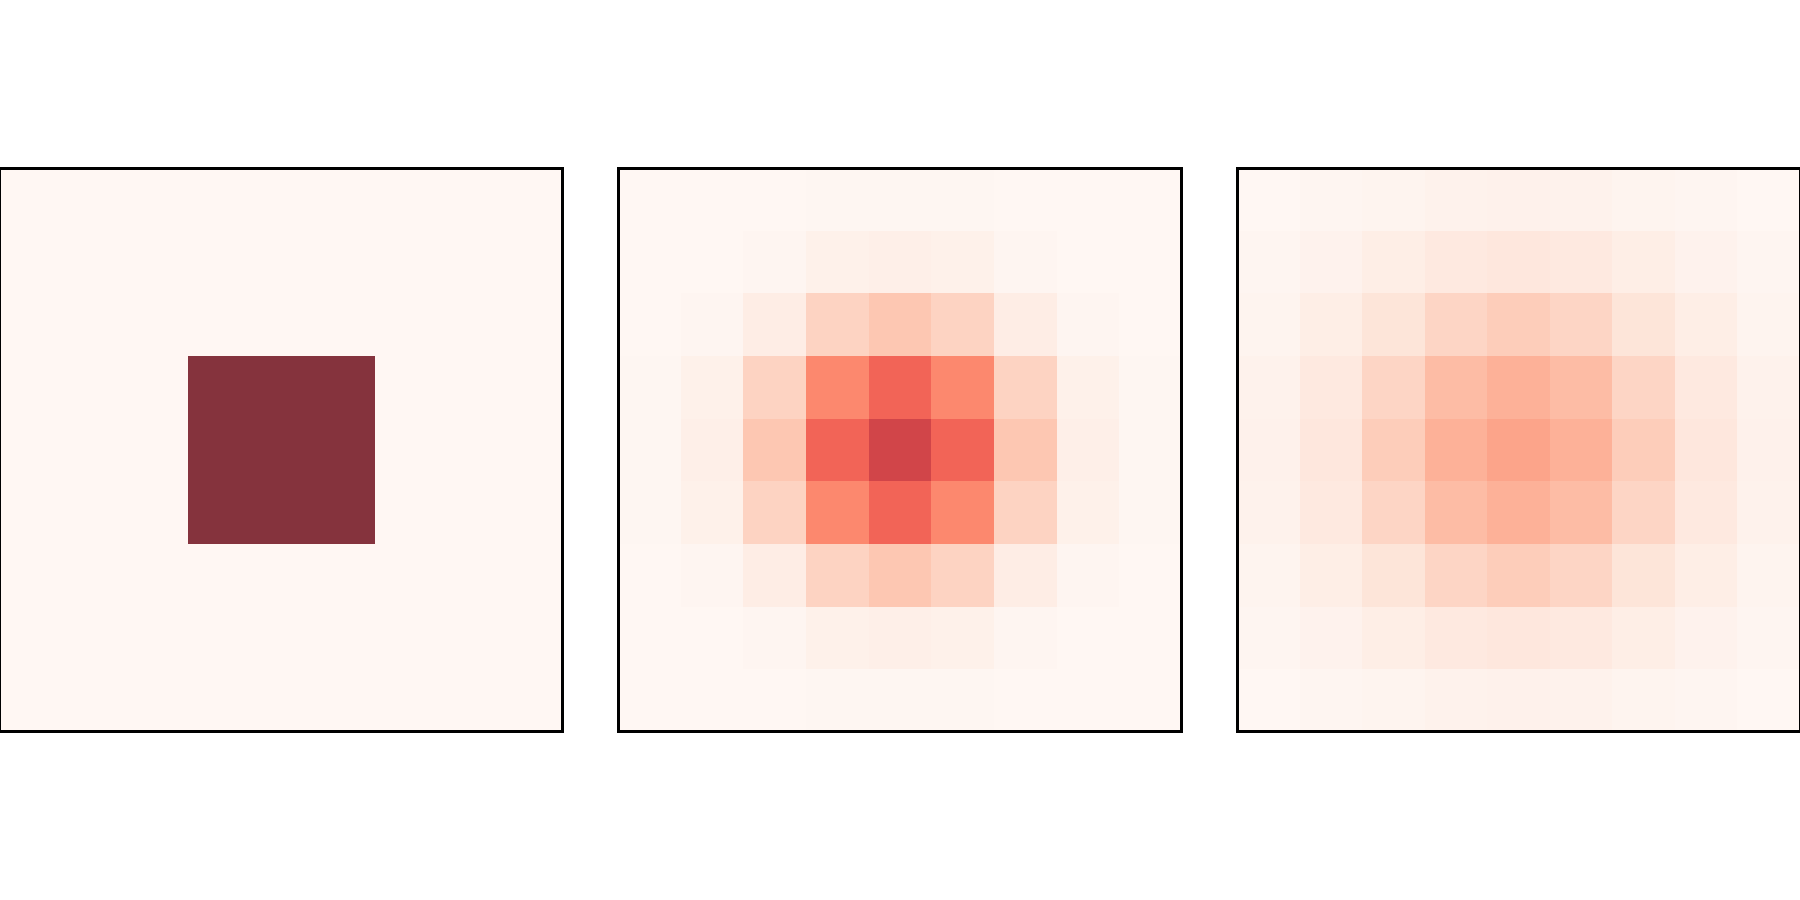
\includegraphics[height=2in]{figs/chap07-1.pdf}}
\caption{A simple diffusion model after 0, 5, and 10 steps.}
\label{chap07-1}
\end{figure}

Figure~\ref{chap07-1} show results for a CA with \py{n=9}, \py{r=0.1}
and initial concentration 0 everywhere except for an ``island'' in the
middle.  The figure shows the starting configuration and the state of
the CA after 5 and 10 steps.  The chemical spreads from the center
outward, continuing until the concentration is the same everywhere.


\section{Reaction-diffusion}

Now let's add a second chemical.  I'll define a new object,
\py{ReactionDiffusion}, that contains two arrays, one for each
chemical:

\begin{code}
class ReactionDiffusion(Cell2D):

   def __init__(self, n, m, params):
        self.params = params
        self.array = np.ones((n, m), dtype=float)
        self.array2 = np.zeros((n, m), dtype=float)
        island(self.array2, val=0.1, noise=0.1)
\end{code}

\py{n} and \py{m} are the number of rows and columns in the array.
\py{params} is a tuple of parameters, which I explain below.

\py{array} represents the concentration of the first chemical, \py{A},
which is initially 1 everywhere.

\py{array2} represents the concentration of \py{B}, which is initially
0 everywhere except an island in the middle, which is initialized
by \py{island}:

\begin{code}
def island(a, val, noise):
    n, m = a.shape
    r = min(n, m) // 20
    a[n//2-r:n//2+r, m//2-r:m//2+r] = val
    a += noise * np.random.random((n, m))
\end{code}

The radius of the island, \py{r}, is one twentieth of \py{n} or \py{m},
whichever is smaller.  The height of the island is \py{val}, which is 0.1
in the example.  Also, random uniform noise, with values from 0 to
\py{noise}, is added to the entire array.

And here is the \py{step} function that updates the arrays:

\begin{code}
    def step(self):
        """Executes one time step."""
        A = self.array
        B = self.array2
        ra, rb, f, k = self.params

        cA = correlate2d(A, self.kernel, **self.options)
        cB = correlate2d(B, self.kernel, **self.options)

        reaction = A * B**2
        self.array += ra * cA - reaction + f * (1-A)
        self.array2 += rb * cB + reaction - (f+k) * B
\end{code}

The parameters are

\begin{description}

\item[\py{ra}:] The diffusion rate of \py{A} (analogous to \py{r} in the
previous section).

\item[\py{rb}:] The diffusion rate of \py{B}.  In most versions of
this model, \py{rb} is about half of \py{ra}.

\item[\py{f}:] The ``feed'' rate, which controls how quickly \py{A} is
added to the system.

\item[\py{k}:] The ``kill'' rate, which controls how quickly \py{B} is
removed from the system.

\end{description}

Now let's look more closely at the update statements:

\begin{code}
        reaction = A * B**2
        self.array += ra * cA - reaction + f * (1-A)
        self.array2 += rb * cB + reaction - (f+k) * B
\end{code}

The arrays \py{cA} and \py{cB} are the result of applying a diffusion
kernel to \py{A} and \py{B}.  Multiplying by \py{ra} and \py{rb} yields
the rate of diffusion into or out of each cell.

The term \py{A * B**2} represents the rate that \py{A} and \py{B}
react with each other.  Assuming that the reaction consumes \py{A} and
produces \py{B}, we subtract this term in the first equation and add
it in the second.

The term \py{f * (1-A)} determines the rate that \py{A} is added to
the system.  Where \py{A} is near 0, the maximum feed rate is \py{f}.
Where \py{A} approaches 1, the feed rate drops off to zero.

Finally, the term \py{(f+k) * B} determines the rate that \py{B} is
removed from the system.  As \py{B} approaches 0, this rate goes
to zero.

As long as the rate parameters are not too high, the values of
\py{A} and \py{B} usually stay between 0 and 1.

\begin{figure}
\centerline{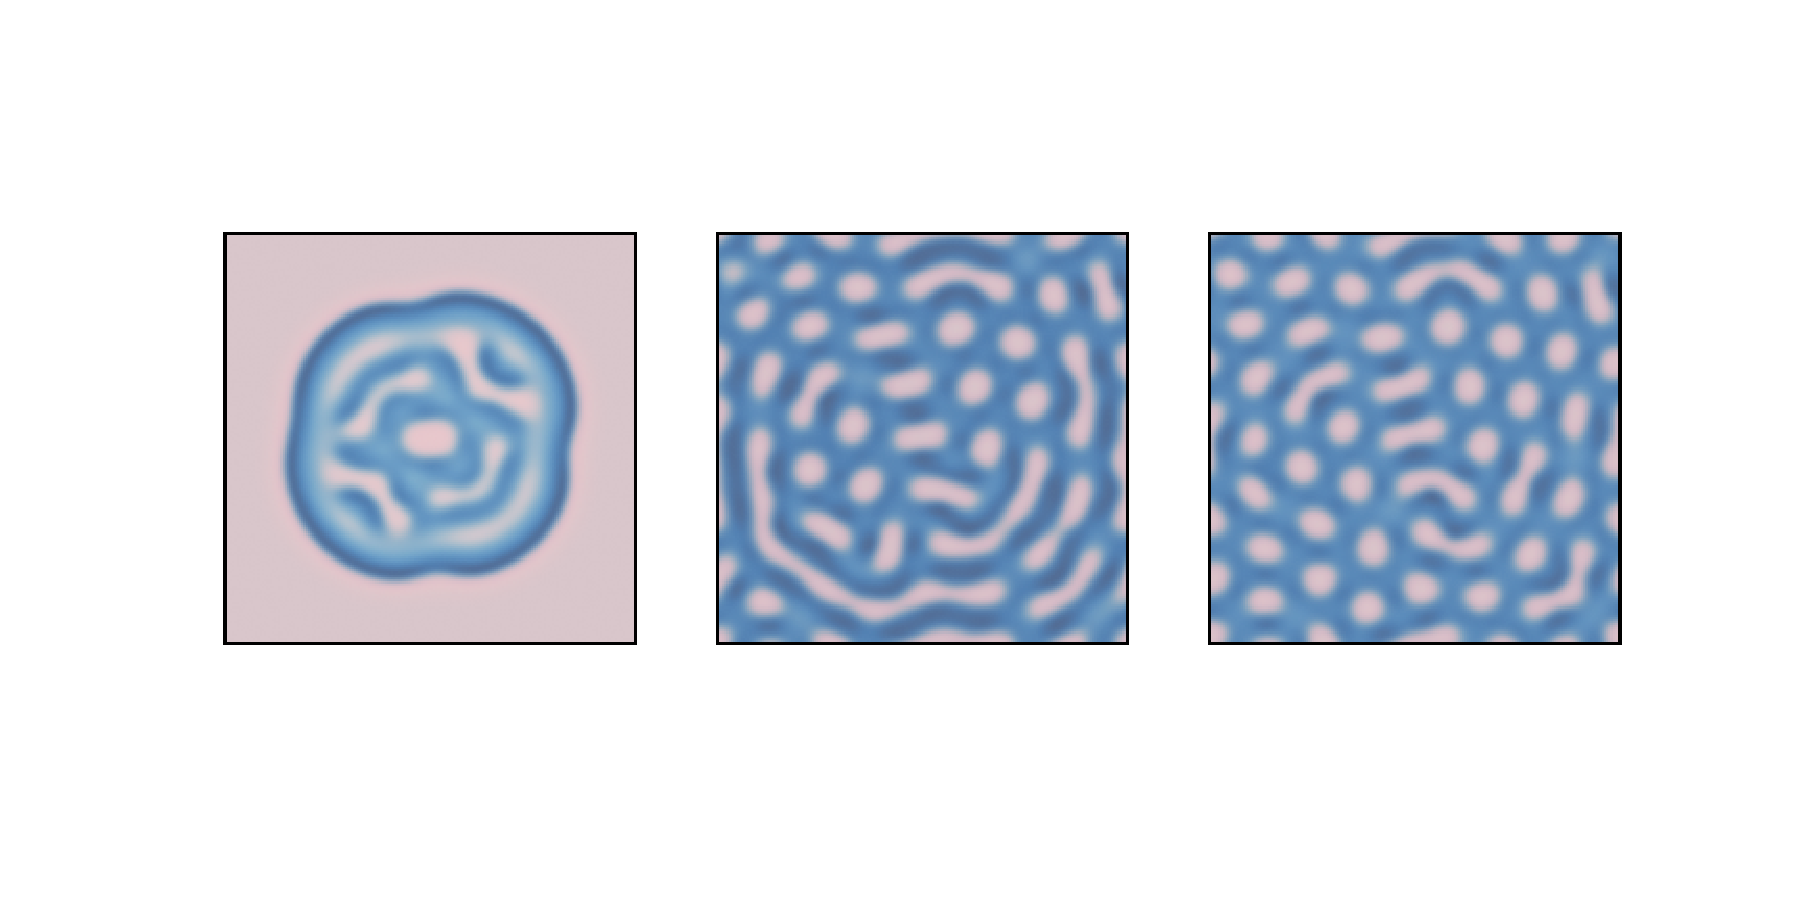
\includegraphics[height=2in]{figs/chap07-2.pdf}}
\caption{Reaction-diffusion model with parameters \py{f=0.035} and
  \py{k=0.057} after 1000, 2000, and 4000 steps.}
\label{chap07-2}
\end{figure}

With different parameters, this model can produce patterns similar
to the stripes and spots on a variety of animals.  In some cases,
the similarity is striking, especially when the feed and
kill parameters vary in space.

For all simulations in this section, \py{ra=0.5} and \py{rb=0.25}.

Figure~\ref{chap07-2} shows results with \py{f=0.035} and
\py{k=0.057}, with the concentration of \py{B} shown in darker colors.
With these parameters, the system evolves toward a stable configuration
with light spots of \py{A} on a dark background of \py{B}.

\begin{figure}
\centerline{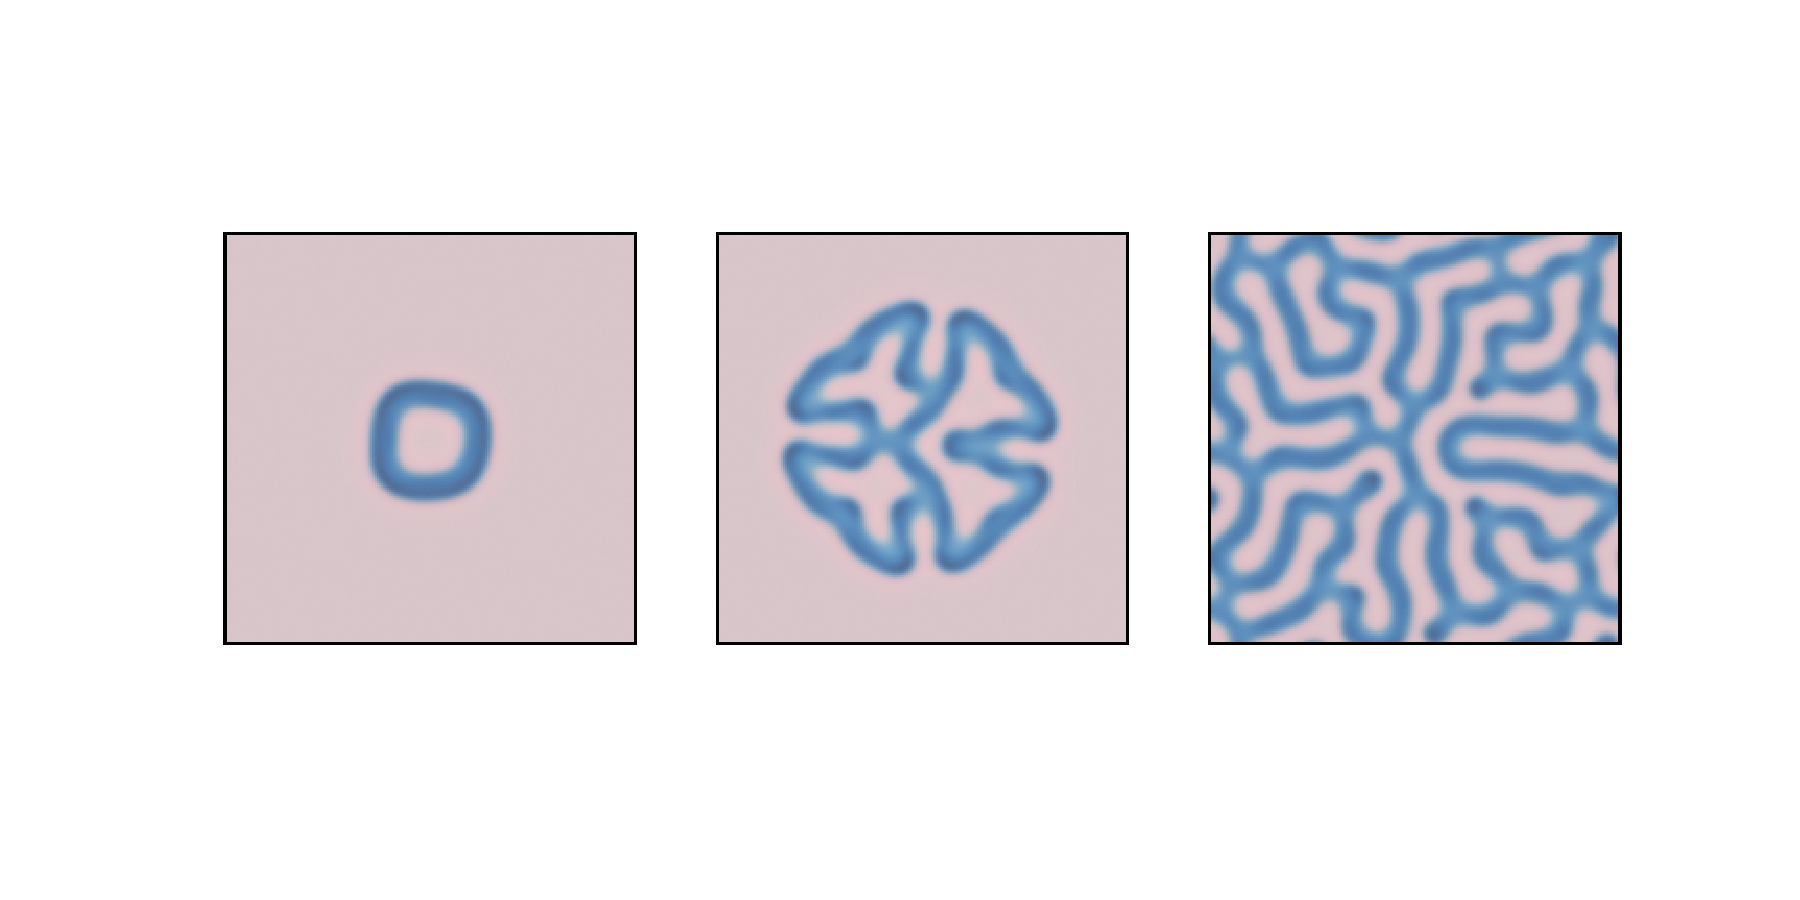
\includegraphics[height=2in]{figs/chap07-3.pdf}}
\caption{Reaction-diffusion model with parameters \py{f=0.055} and
  \py{k=0.062} after 1000, 2000, and 4000 steps.}
\label{chap07-3}
\end{figure}

Figure~\ref{chap07-3} shows results with \py{f=0.055} and
\py{k=0.062} which yields a coral-like pattern of \py{B} on a background
of \py{A}.

\begin{figure}
\centerline{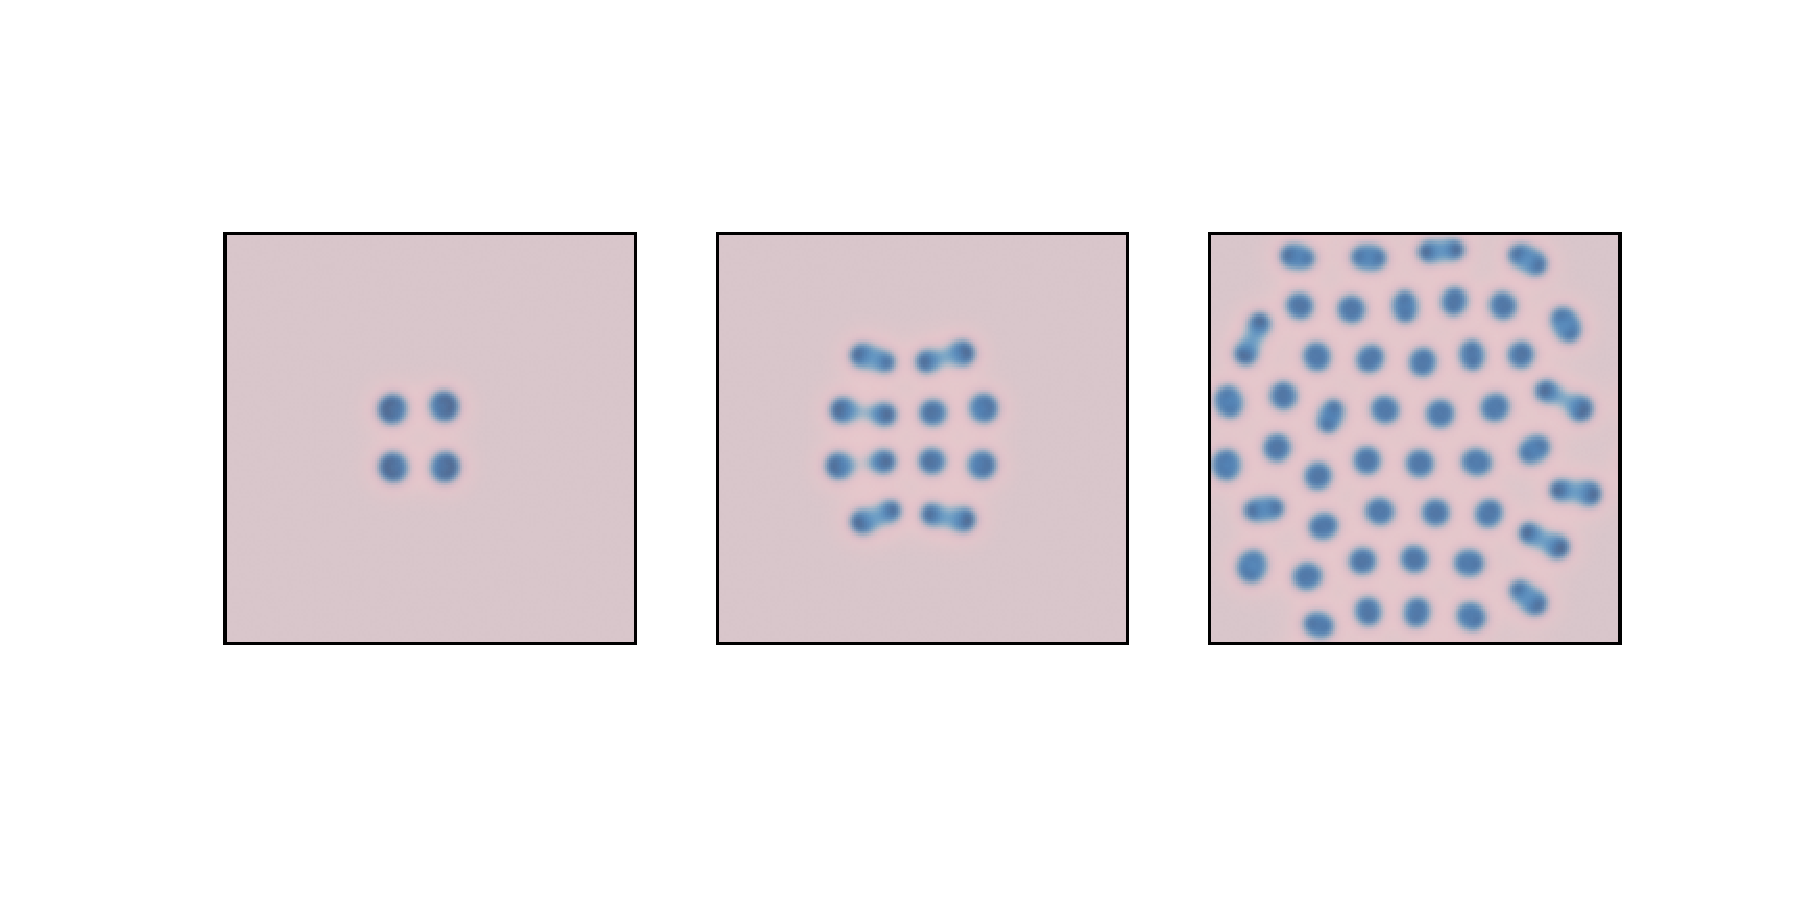
\includegraphics[height=2in]{figs/chap07-4.pdf}}
\caption{A reaction-diffusion model with parameters \py{f=0.039} and
  \py{k=0.065} after 1000, 2000, and 4000 steps.}
\label{chap07-4}
\end{figure}

Figure~\ref{chap07-4} shows results with \py{f=0.039} and
\py{k=0.065}.  These parameters produce spots of \py{B} that grow and
divide in a process that resembles mitosis, ending with a stable pattern
of equally-spaced spots.

Since 1952, observations and experiments have provided some support
for Turing's conjecture.  At this point it seems likely, but not yet
proven, that many animal patterns are actually formed by
reaction-diffusion processes of some kind.


\section{Percolation}

Percolation is a process in which a fluid flows through a semi-porous
material.  Examples include oil in rock formations, water in paper,
and hydrogen gas in micropores.  Percolation models are also used to
study systems that are not literally percolation, including epidemics
and networks of electrical resistors.  See
\url{http://en.wikipedia.org/wiki/Percolation_theory}.

\index{percolation}

Percolation models are often represented using random graphs like the
ones we saw in Chapter~\ref{graphs}, but they can also be represented
using cellular automatons.  In the next few sections we'll explore
a 2-D CA that simulates percolation.

In this model:

\begin{itemize}

\item Initially, each cell is either ``porous'' with probability \py{p} or
``non-porous'', and all cells are considered ``dry'' except the top
row, which is ``wet''.

\item During each time step, if a porous cell has at least one wet neighbor,
it becomes wet.  Non-porous cells stay dry.

\item The simulation runs until it reaches a ``fixed point'' where no
more cells change state.

\end{itemize}

If there is a path of wet cells from the top to the bottom row, we say
that the CA has a ``percolating cluster''.

One of the primary questions of interest regarding percolation is the
probability of finding a percolating cluster and how it depends on
\py{p}.  This question might remind you of Section~\ref{randomgraphs},
where we computed the probability that a random \Erdos-\Renyi~graph is
connected.  We will see several connections between that model and
this one.

I define a new class to represent a percolation model:

\begin{code}
class Percolation(Cell2D):

    def __init__(self, n, m, p):
        self.p = p
        self.array = np.random.choice([0, 1], (n, m), p=[1-p, p])
        self.array[0] = 5
\end{code}

\py{n} and \py{m} are the number of rows and columns in the CA.  \py{p}
is the probability that a cell is porous.

The state of the CA is stored in \py{array}, which is initialized
using \py{np.random.choice} to choose 1 (porous) with probability
\py{p}, and 0 (non-porous) with probability \py{1-p}.
The state of the top row is set to 5, which represents a wet cell.

During each time step, we check whether any porous cell has a wet
neighbor, using a 4-cell neighborhood (not including the diagonals).
Here is the kernel:

\begin{code}
    kernel = np.array([[0, 1, 0],
                       [1, 0, 1],
                       [0, 1, 0]])
\end{code}

And here is the \py{step} function:


\begin{code}
    def step(self):
        a = self.array
        c = correlate2d(a, self.kernel, mode='same')
        self.array[(a==1) & (c>=5)] = 5
\end{code}

\py{correlate2d} adds up the state of the neighbors, which can only
exceed 5 if at least one neighbor is wet.  The last line finds cells
that are porous, \py{a==1}, with at least one wet neighbor, \py{c>=5},
and sets their state to 5, which is wet.

\begin{figure}
\centerline{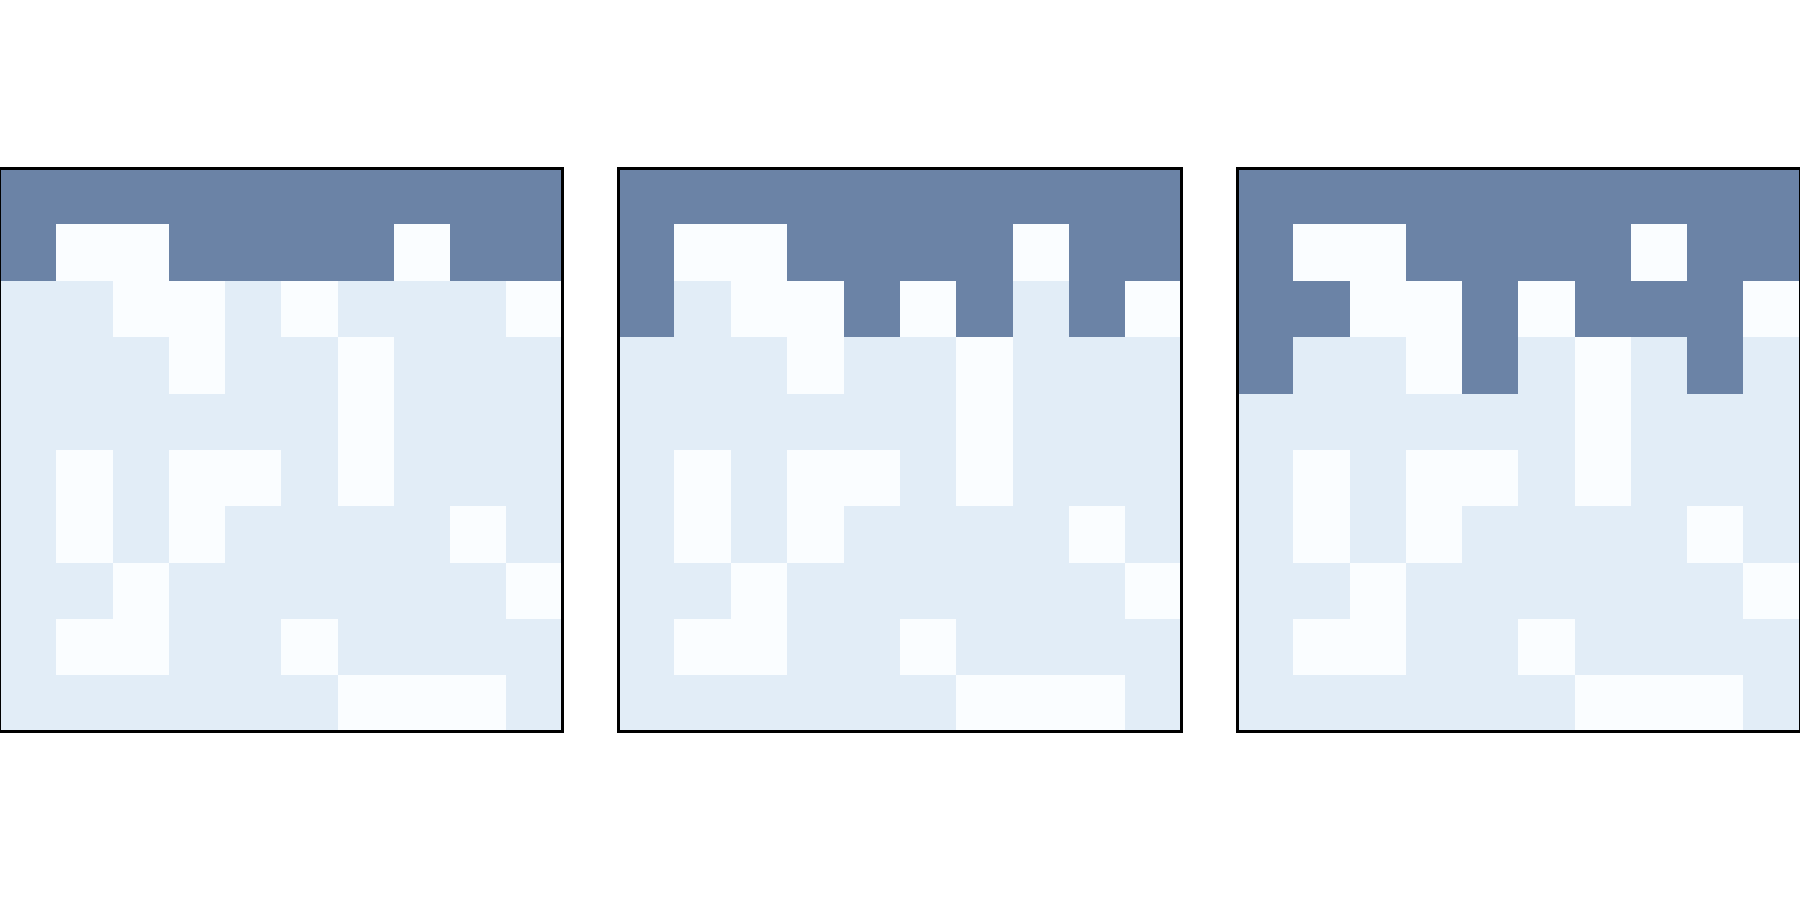
\includegraphics[height=2in]{figs/chap07-5.pdf}}
\caption{The first three steps of a percolation model with \py{n=10} and
\py{p=0.5}.}
\label{chap07-5}
\end{figure}

Figure~\ref{chap07-5} shows the first few steps of a percolation model
with \py{n=10} and \py{p=0.5}.  Non-porous cells are white, porous cells
are lightly shaded, and wet cells are dark.


\section{Phase change}

Now let's test whether a CA contains a percolating cluster:

\begin{code}
def test_perc(perc):
    num_wet = perc.num_wet()

    num_steps = 0
    while True:
        perc.step()
        num_steps += 1

        if perc.bottom_row_wet():
            return True, num_steps

        new_num_wet = perc.num_wet()
        if new_num_wet == num_wet:
            return False, num_steps

        num_wet = new_num_wet
\end{code}

\py{test_perc} takes a \py{Percolation} object as a parameter.  Each
time through the loop, it advances the CA one time step.  It
checks the bottom row to see if any cells are wet; if so,
it returns \py{True}, to indicate that there is a percolating cluster,
and \py{num_steps}, which is the number of time steps it took to
get to the bottom.

During each time step, it also computes the number of wet cells and
checks whether the number increased since the last step.  If not, we
have reached a fixed point without finding a percolating cluster, so
we return \py{False}.

To estimate the probability of a percolating cluster, we generate
many random initial configurations and test them:

\begin{code}
def estimate_prob_percolating(p=0.5, n=100, iters=100):
    count = 0
    for i in range(iters):
        perc = Percolation(n, p=p)
        flag, _ = test_perc(perc)
        if flag:
            count += 1

    return count / iters
\end{code}

\py{estimate_prob_percolating} makes 100 CAs with the given values of
\py{p} and \py{n} and calls \py{test_perc} to see how many of them
have a percolating cluster.  The return value is the fraction of CAs
that do.

When \py{p=0.55}, the probability of a percolating cluster is near 0.
At \py{p=0.60}, it is about 70\%, and at \py{p=0.65} it is near 1.
This rapid transition indicates that there is a critical value of
\py{p} near 0.6.

We can estimate the critical value more precisely using a random
walk.  Starting from an initial value of \py{p}, we construct a
\py{Percolation} object and check whether it has a percolating cluster.
If so, \py{p} is probably too high, so we decrease it.  If not,
\py{p} is probably too low, so we increase it.

Here's the code:

\begin{code}
def find_critical(p=0.6, n=100, iters=100):
    ps = [p]
    for i in range(iters):
        perc = Percolation(n=n, p=p)
        flag, _ = test_perc(perc)
        if flag:
            p -= 0.005
        else:
            p += 0.005
        ps.append(p)
    return ps
\end{code}

\py{find_critical} starts with the given value of \py{p} and adjusts
up and down, returning the list of values.  With \py{n=100} the
average of \py{ps} is about 0.59, and this critical value seems to
be the same for values of \py{n} from 50 to 400.

The rapid change in behavior near the critical value is
called a {\bf phase change} by analogy with phase changes
in physical systems, like the way water changes from liquid to
solid at its freezing point.

A wide variety of systems display a common set of behaviors and
characteristics when they are at or near a critical point.
These behaviors are known collectively as {\bf critical phenomena}.
In the next section, we explore one of them: fractal geometry.


\section{Fractals}
\label{fractals}

To understand fractals, we have to start with dimensions.

For simple geometric objects, dimension is defined in terms of scaling
behavior.  For example, if the side of a square has length $l$, its
area is $l^2$.  The exponent, 2, indicates that a square is
2-dimensional.  Similarly, if the side of a cube has length $l$, its
volume is $l^3$, which indicates that a cube is 3-dimensional.

More generally, we can estimate the dimension of an object by
measuring its ``size'' (by some definition) as a function of
a linear measure.

As an example, I'll estimate the dimension of a 1-D cellular
automaton by measuring its area (total number of ``on'' cells)
as a function of the number of rows.

\index{fractal dimension}

\begin{figure}
\centerline{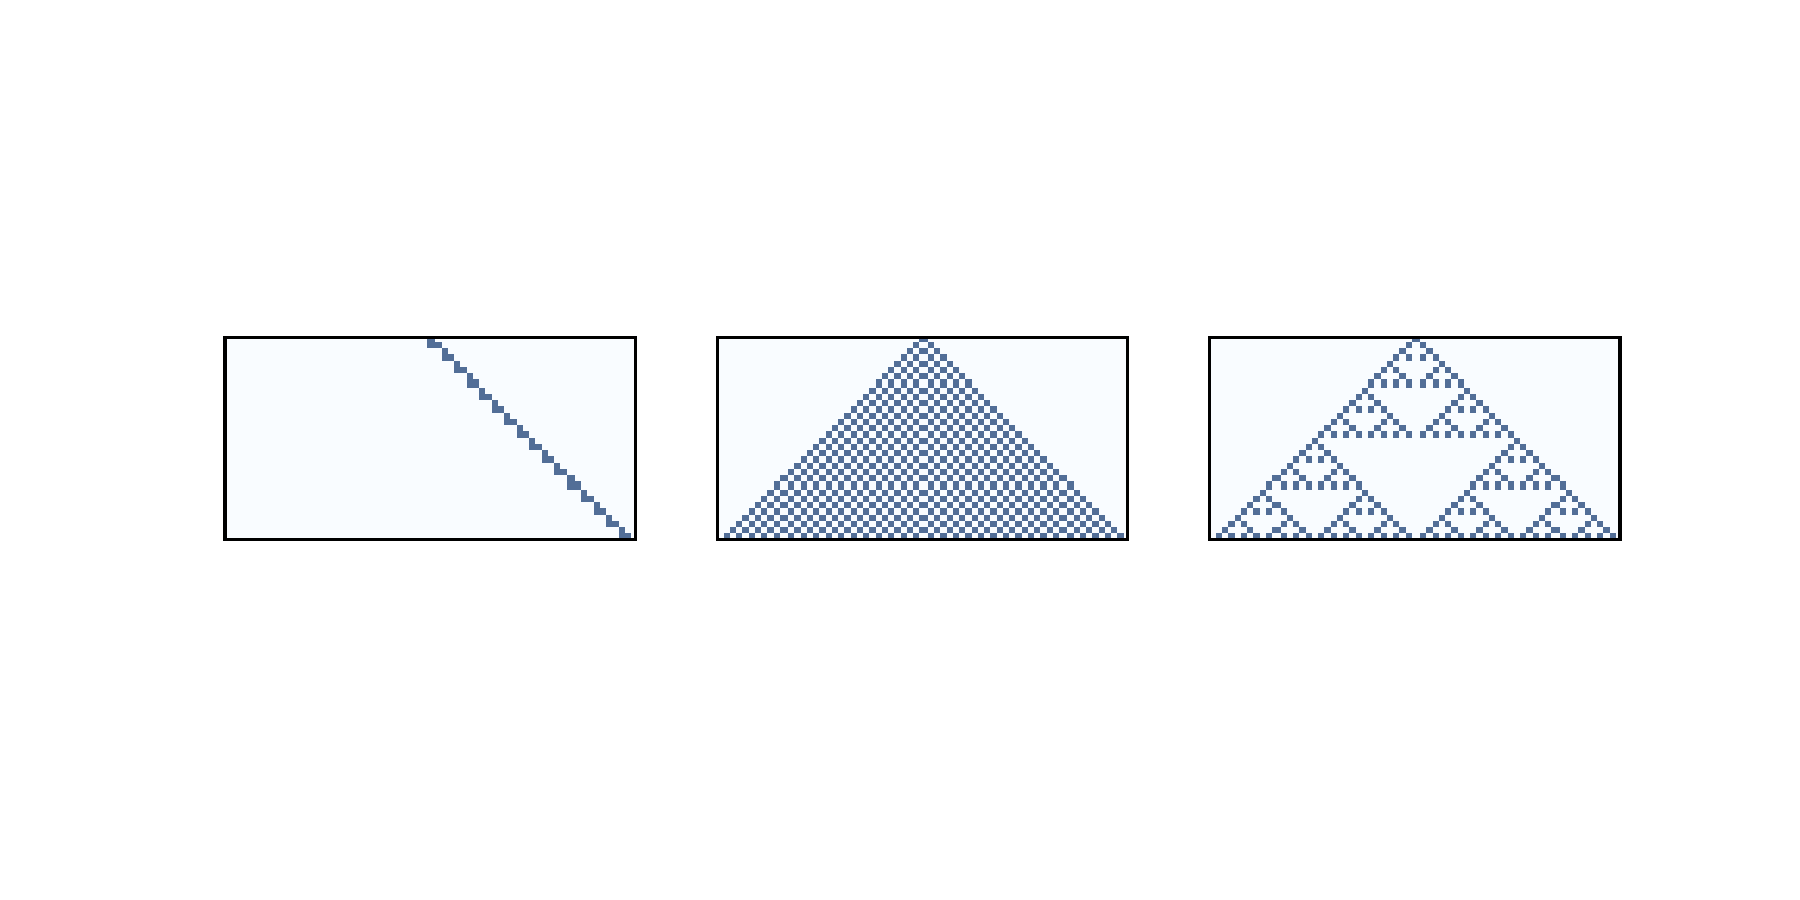
\includegraphics[height=2in]{figs/chap07-7.pdf}}
\caption{One-dimensional CAs with rules 20, 50, and 18, after 32 time steps.}
\label{chap07-7}
\end{figure}

Figure~\ref{chap07-7} shows three 1-D CAs like the ones we saw
in Section~\ref{onedim}.  Rule 20 (left) generates
a set of cells that seems linear, so we expect it to be one-dimensional.  Rule 50 (center) produces something like a triangle, so
we expect it to be 2-D.  Rule 18 (right) also produces something like a
triangle, but the density is not uniform, so its scaling behavior is
not obvious.

I'll estimate the dimension of these CAs with the following function,
which counts the number of on cells after each time step.
It returns a list of tuples, where each tuple contains $i$ and
$i^2$, for purposes of comparison, and the total number of cells.

\begin{code}
def count_cells(rule, n=500):
    ca = Cell1D(rule, n)
    ca.start_single()

    res = []
    for i in range(1, n):
        cells = np.sum(ca.array)
        res.append((i, i**2, cells))
        ca.step()

    return res
\end{code}

\begin{figure}
\centerline{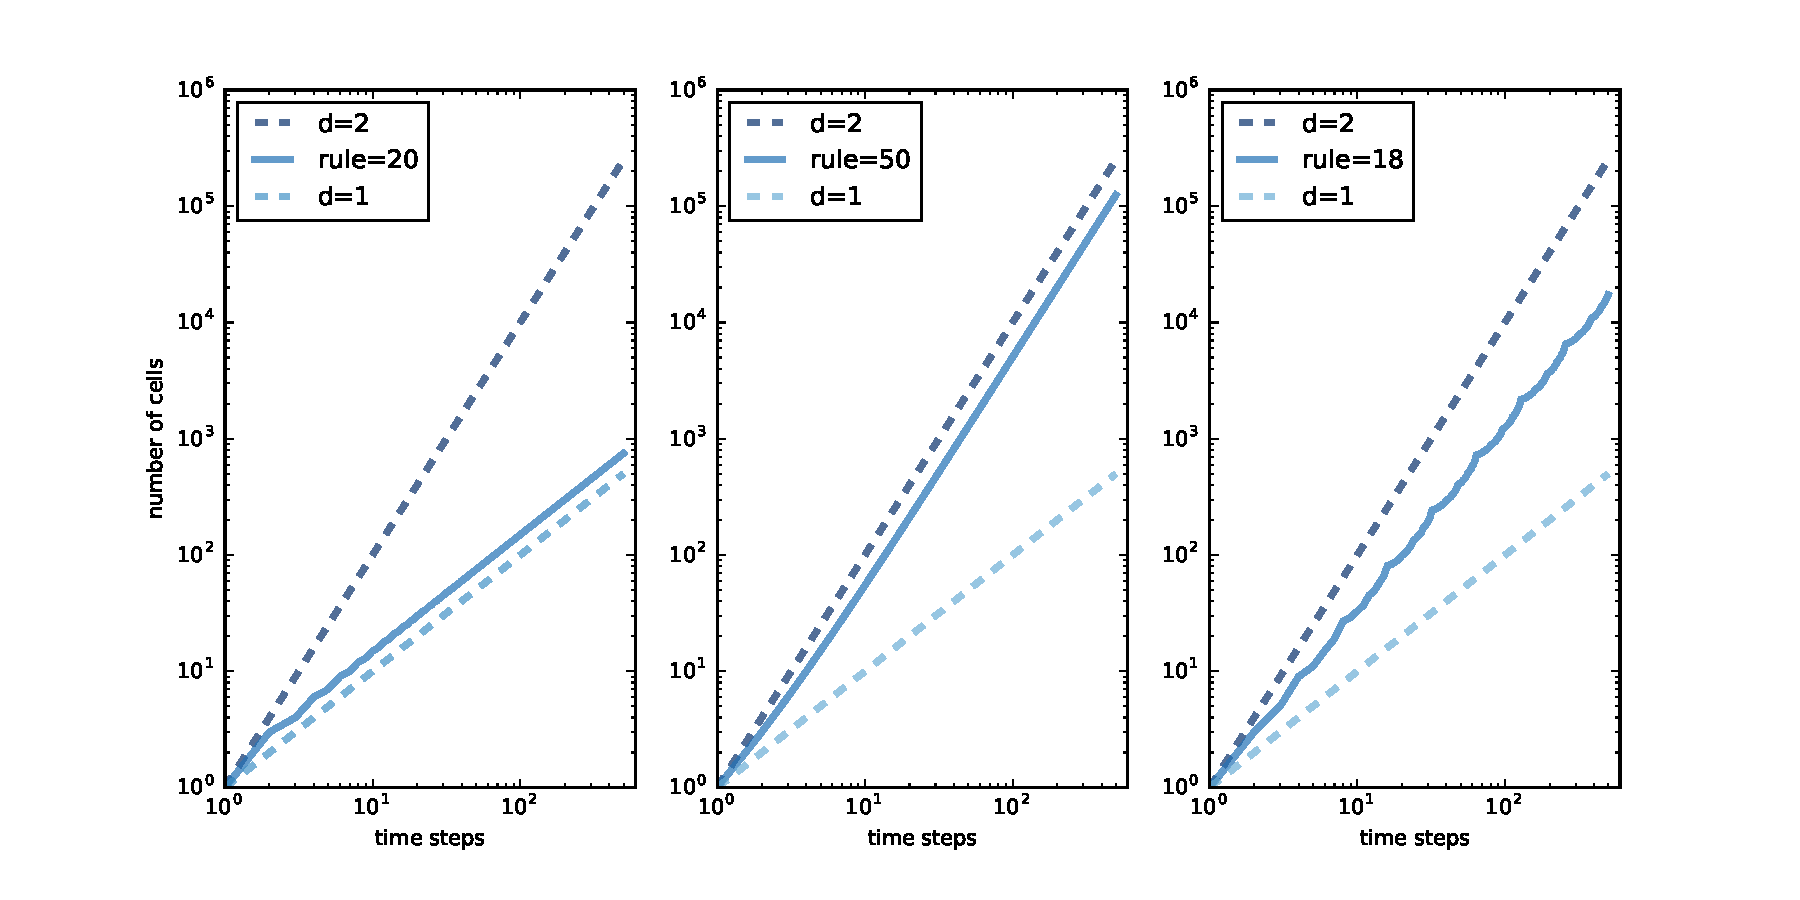
\includegraphics[height=2in]{figs/chap07-8.pdf}}
\caption{Number of ``on'' cells versus number of time steps for
rules 20, 50, and 18.}
\label{chap07-8}
\end{figure}

Figure~\ref{chap07-8} shows the results plotted on a log-log scale.

In each figure, the top dashed line shows $y = i^2$.  Taking
the log of both sides, we have $\log y = 2 \log i$.  Since the
figure is on a log-log scale, the slope of this line is 2.

Similarly, the bottom dashed line shows $y = i$.  On a log-log
scale, the slope of this line is 1.

Rule 20 (left) produces 3 cells every 2 time steps, so the total number
of cells after $i$ steps is $y = 1.5 i$.  Taking the log of both
sides, we have $\log y = \log 1.5 + \log i$, so on a log-log
scale, we expect a line with slope 1.  In fact, the estimated
slope of the line is 1.01.

Rule 50 (center) produces $i+1$ new cells during the $i$th time step,
so the total number of cells after $i$ steps is $y = i^2 + i$.  If we
ignore the second term and take the log of both sides, we have $\log y
\sim 2 \log i$, so as $i$ gets large, we expect to see a line with
slope 2.  In fact, the estimated slope is 1.97.

Finally, for Rule 18 (right), the estimated slope is about 1.57, which
is clearly not 1, 2, or any other integer.  This suggests that the
pattern generated by Rule 18 has a ``fractional dimension''; that is,
it is a fractal.


\section{Fractals and Percolation Models}
\label{fracperc}

\begin{figure}
\centerline{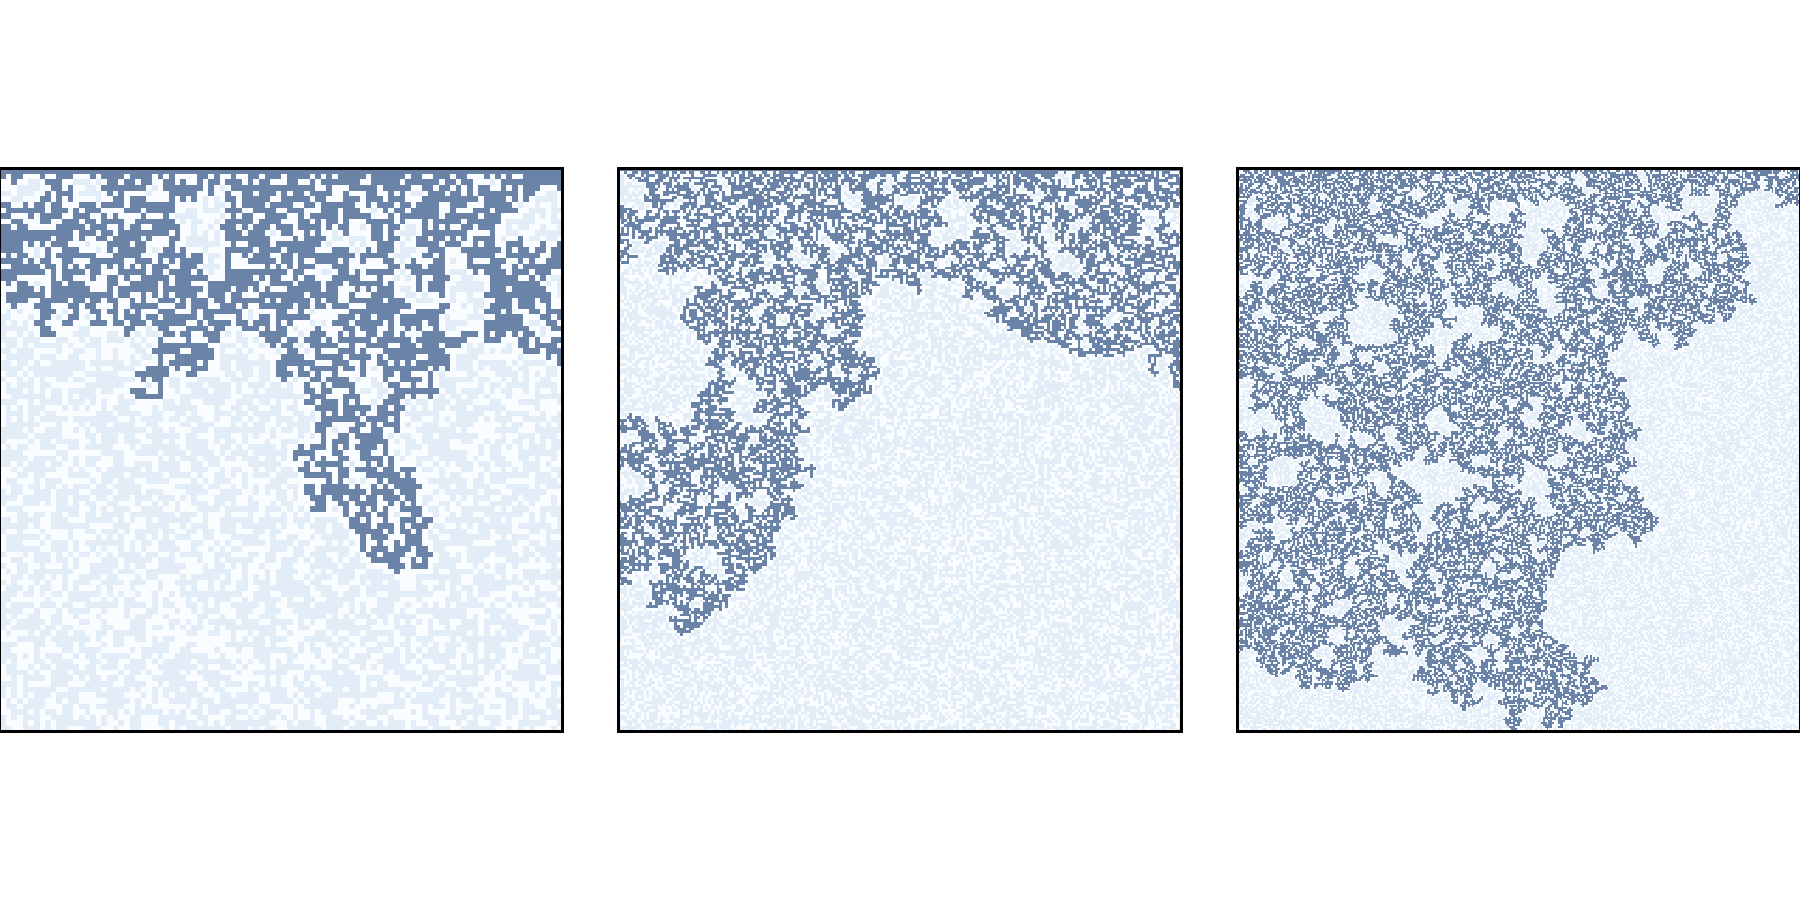
\includegraphics[height=2in]{figs/chap07-6.pdf}}
\caption{Percolation models with \py{p=0.6} and \py{n=100},
\py{200}, and \py{300}.}
\label{chap07-6}
\end{figure}

Now let's get back to percolation models.  Figure~\ref{chap07-6} shows
clusters of wet cells in percolation simulations with \py{p=0.6} and
\py{n=100}, \py{200}, and \py{300}.  Informally, they resemble fractal
patterns seen in nature and in mathematical models.

To estimate their fractal dimension, we can run CAs with
a range of sizes, count the number of wet cells in each percolating
cluster, and then see how the cell counts scale as we increase the
size of the CA.

The following loop runs the simulations:

\begin{code}
    for size in sizes:
        perc = Percolation(size, p=p)
        flag, _ = test_perc(perc)
        if flag:
            num_filled = perc.num_wet() - size
            res.append((size, size**2, num_filled))
\end{code}

The result is a list of tuples where each tuple contains \py{size}
and \py{size**2}, for comparison, and the number of cells in the
percolating cluster (not including the initial wet cells in the top
row).

\begin{figure}
\centerline{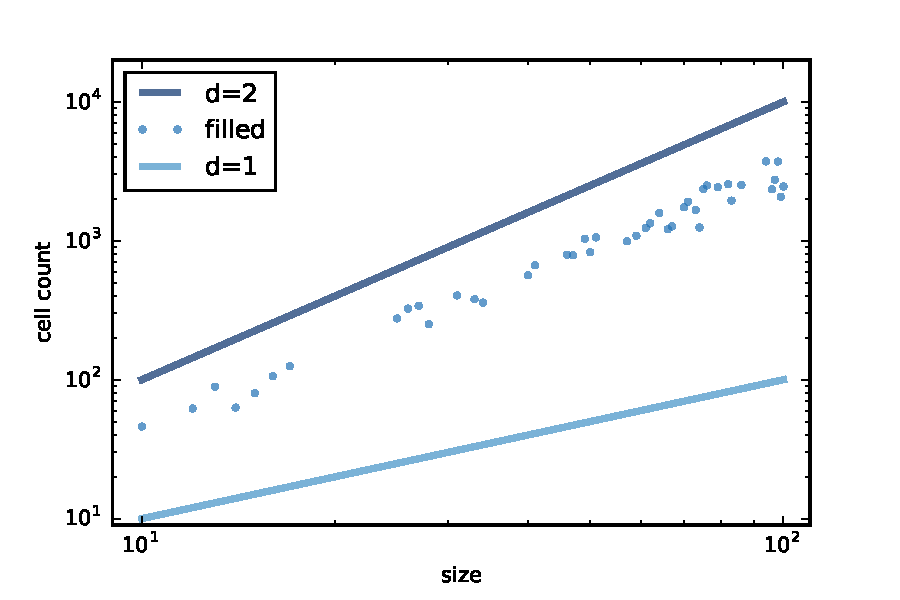
\includegraphics[height=2in]{figs/chap07-9.pdf}}
\caption{Number of cells in the percolating cluster versus CA size.}
\label{chap07-9}
\end{figure}

Figure~\ref{chap07-9} shows the results for a range of sizes from 10
to 100.  The dots show the number of cells in each percolating
cluster.  The slope of a line fitted to these dots is about 1.85,
which indicates that the percolating cluster is, in fact, fractal when
\py{p} is near the critical value.

When \py{p} is larger than the critical value, nearly every porous
cell gets filled, so the number of wet cells is just \py{p * size^2},
which has dimension 2.

When \py{p} is substantially smaller than the critical value, the number
of wet cells is proportional to the linear size of the CA, so it has
dimension 1.


\section{Exercises}


\begin{exercise}

In Section~\ref{fracperc} we showed that the Rule 18 CA produces a fractal.
Can you find other 1-D CAs that produce fractals?

Note: the \py{Cell1D} object in \py{Cell1D.py} does not wrap around
from the left edge to the right, which creates artifacts at the
boundaries for some rules.  You might want to use \py{Wrap1D}, which
is a child class of \py{Cell1D} that wraps around.  It is also defined
in \py{Cell1D.py}.

\end{exercise}


\begin{exercise}

In 1990 Bak, Chen and Tang proposed a cellular automaton that is
an abstract model of a forest fire.  Each cell is in one of three
states: empty, occupied by a tree, or on fire.
\index{Bak, Per}
\index{forest fire model}

The rules of the CA are:

\begin{enumerate}

\item An empty cell becomes occupied with probability $p$.

\item A cell with a tree burns if any of its neighbors
  is on fire.

\item A cell with a tree spontaneously burns, with
  probability $f$, even if none of its neighbors is on fire.

\item A cell with a burning tree becomes an empty cell in the next
  time step.

\end{enumerate}

Write a program that implements this model.  You might want to inherit
from \py{Cell2D}.  Typical values for the parameters are $p=0.01$ and
$f=0.001$, but you might want to experiment with other values.

Starting from a random initial condition, run the CA until it reaches
a steady state where the number of trees no longer increases or
decreases consistently.

In steady state, is the geometry of the forest fractal?
What is its fractal dimension?

\end{exercise}






\chapter{Self-organized criticality}
\label{soc}

In the previous chapter we saw an example of a system with a critical
point and we explored one of the common properties of critical
systems, fractal geometry.

In this chapter, we explore two other properties of critical systems:
heavy-tailed distributions, which we saw in Chapter~\ref{heavytail}
and pink noise, which I'll explain in this chapter.

These properties are interesting in part because they appear
frequently in nature; that is, many natural systems produce
fractal-like geometry, heavy-tailed distributions, and pink noise.

This observation raises a natural question: why do so many natural
systems have properties of critical systems?  A possible answer is
{\bf self-organized criticality} (SOC), which is the tendency of some
systems to evolve toward and stay in a critical state.

In this chapter I'll present a {\bf sand pile model}, which was the
first system shown to exhibit SOC.

The code for this chapter is in {\tt chap08.ipynb} in the repository
for this book.  More information about working with the code is
in Section~\ref{code}.


\section{Critical Systems}

Many critical systems demonstrate common behaviors:

\begin{itemize}

\item Fractal geometry: For example, freezing water tends to form
  fractal patterns, including snowflakes and other crystal
  structures.  Fractals are characterized by self-similarity; that is,
  parts of the pattern are similar to scaled copies of the whole.

\index{fractal geometry}
\index{self-similarity}

\item Heavy-tailed distributions of some physical quantities: For
  example, in freezing water the distribution of crystal sizes is
  characterized by a power law.

\index{long tail}
\index{power law}

\item Variations in time that exhibit {\bf pink noise}.  Complex
  signals can be decomposed into their frequency components.  In pink
  noise, low-frequency components have more power than high-frequency
  components.  Specifically, the power at frequency $f$ is
  proportional to $1/f$.

\index{pink noise}
\index{1/f noise@$1/f$ noise}

\end{itemize}

Critical systems are usually unstable.  For example, to keep water in
a partially frozen state requires active control of the temperature.
If the system is near the critical temperature, a small deviation
tends to move the system into one phase or the other.

\index{unstable}

Many natural systems exhibit characteristic behaviors of criticality,
but if critical points are unstable, they should not be common in
nature.  This is the puzzle Bak, Tang and Wiesenfeld address.  Their
solution is called self-organized criticality (SOC), where
``self-organized'' means that from any initial condition, the system
moves toward a critical state, and stays there, without
external control.

\index{SOC}

\section{Sand Piles}

The sand pile model was proposed by Bak, Tang and Wiesenfeld in 1987.
It is not meant to be a realistic model of a sand pile, but rather an
abstraction that models physical systems with (1) a large number of
elements that (2) interact with their neighbors.

\index{sand pile model}
\index{abstract model}

The sand pile model is a 2-D cellular automaton where the state of
each cell represents the slope of a part of a sand pile.  During each
time step, each cell is checked to see whether it exceeds a critical
value, $K$, which is usually 3.  If so, it ``topples'' and transfers
sand to four neighboring cells; that is, the slope of the cell is
decreased by 4, and each of the neighbors is increased by 1.
At the perimeter of the grid, all cells are kept at slope 0, so the
excess spills over the edge.

\index{2-D cellular automaton} \index{state}

Bak, Tang and Wiesenfeld initialize all cells at a
level greater than \py{K} and run the model until it stabilizes.
Then they observe the effect of small perturbations; they choose a
cell at random, increment its value by 1, and run the model,
again, until it stabilizes.

\index{grid}

For each perturbation, they measure \py{T}, the number of time steps
the pile takes to stabilize, and \py{S}, the total number of cells
that topple\footnote{The original paper uses a different definition
of \py{S}, but most later work uses this definition.}.

Most of the time, dropping a single grain causes no cells to topple,
so \py{T=1} and \py{S=0}.  But occasionally a single grain can cause an
{\bf avalanche} that affects a substantial fraction of the grid.  The
distributions of \py{T} and \py{S} turn out to be heavy-tailed, which
supports the claim that the system is in a critical state.

\index{avalanche}

They conclude that the sand pile model exhibits ``self-organized
criticality'', which means that from the initial condition it evolves
toward a critical state without the need for external control or
what they call ``fine tuning'' of any parameters.  And the model
stays in a critical state as more grains are added.

In the next few sections I replicate their experiments and
interpret the results.


\section{Implementing the Sand Pile}

To implement the sand pile model, I define a class called \py{SandPile}
that inherits from \py{Cell2D}, which is defined in \py{Cell2D.py}.

\begin{code}
class SandPile(Cell2D):

    def __init__(self, n, m, level=9):
        self.array = np.ones((n, m)) * level
\end{code}

All values in the array are initialized to \py{level}, which is
generally greater than the toppling threshold, \py{K}.

Here's the \py{step} method that finds all cells above \py{K} and
topples them:

\begin{code}
    kernel = np.array([[0, 1, 0],
                       [1,-4, 1],
                       [0, 1, 0]], dtype=np.int32)

    def step(self, K=3):
        toppling = self.array > K
        num_toppled = np.sum(toppling)
        c = correlate2d(toppling, self.kernel, mode='same')
        self.array += c
        return num_toppled
\end{code}

To explain how that works, I'll start with
a small pile with just two cells ready to topple:

\begin{code}
pile = SandPile(n=3, m=5, level=0)
pile.array[1, 1] = 4
pile.array[1, 3] = 4
\end{code}

Initially, \py{pile.array} looks like this:

\begin{code}
[[0 0 0 0 0]
 [0 4 0 4 0]
 [0 0 0 0 0]]
\end{code}

Now we can select the cells that are above the toppling threshold:

\begin{code}
toppling = pile.array > K
\end{code}

The result is an array of booleans, but we can use it as if it were
an array of integers like this:

\begin{code}
[[0 0 0 0 0]
 [0 1 0 1 0]
 [0 0 0 0 0]]
\end{code}

If we correlate this array with the kernel, it makes copies of the
kernel at each location where \py{toppling} is 1.

\begin{code}
c = correlate2d(toppling, kernel, mode='same')
\end{code}

And here's the result:

\begin{code}
[[ 0  1  0  1  0]
 [ 1 -4  2 -4  1]
 [ 0  1  0  1  0]]
\end{code}

Notice that where the copies of the kernel overlap, they add up.

This array contains the change for each cell, which we use
to update the original array:

\begin{code}
pile.array += c
\end{code}

And here's the result.

\begin{code}
[[0 1 0 1 0]
 [1 0 2 0 1]
 [0 1 0 1 0]]
\end{code}

So that's how \py{step} works.

By default, \py{correlate2d} considers the boundary of the array
to be fixed at zero, so any grains of sand that go over the edge
disappear.

\py{SandPile} also provides \py{run}, which calls step until
no more cells topple:

\begin{code}
    def run(self):
        total = 0
        for i in itertools.count(1):
            num_toppled = self.step()
            total += num_toppled
            if num_toppled == 0:
                return i, total
\end{code}

The return value is a tuple that contains the number of time
steps and the total number of cells that toppled.

If you are not familiar with \py{itertools.count}, it is an
infinite generator that counts up from the given initial value,
so the \py{for} loop runs until \py{step} returns 0.

Finally, the \py{drop} method chooses a random cell and adds a
grain of sand:

\begin{code}
    def drop(self):
        a = self.array
        n, m = a.shape
        index = np.random.randint(n), np.random.randint(m)
        a[index] += 1
\end{code}

Let's look at a bigger example, with \py{n=20}:

\begin{code}
pile = SandPile(n=20, level=10)
pile.run()
\end{code}

\begin{figure}
\centerline{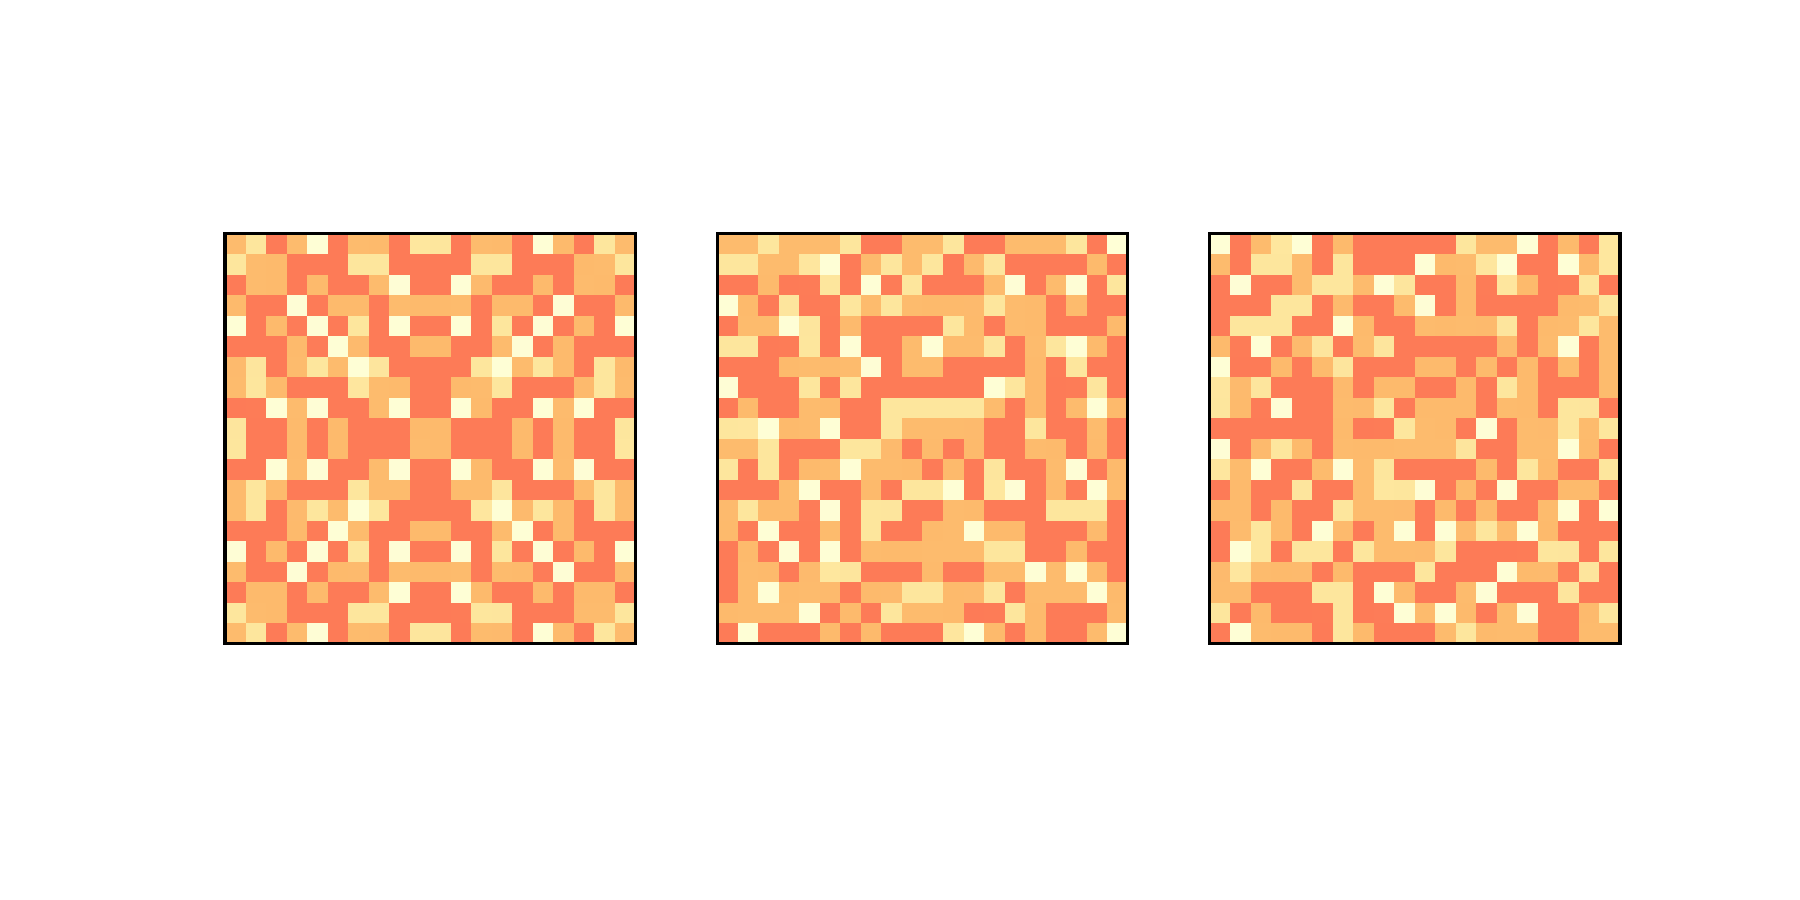
\includegraphics[height=3in]{figs/chap08-1.pdf}}
\caption{Sand pile model initial state (left), after 200 steps (middle), and 400 steps (right).}
\label{chap08-1}
\end{figure}

With an initial level of \py{10}, this sand pile takes 332 time steps to
reach equilibrium, with a total of 53,336 topplings.
Figure~\ref{chap08-1} (left) show the configuration, after this initial
run.  Notice that it has the repeating elements that
are characteristic of fractals.  We'll come back to that soon.

Figure~\ref{chap08-1} (middle) shows the configuration of the sand
pile after dropping 200 grains onto random cells, each time running
until the pile reaches equilibrium.  The symmetry of the initial
configuration has been broken; the configuration looks random.

Finally Figure~\ref{chap08-1} (right) shows the configuration
after 400 drops.  It looks similar to the configuration after 200
drops.  In fact, the pile is now in a steady state where its statistical
properties don't change over time.  I'll explain some of those
statistical properties in the next section.


\section{Heavy-tailed distributions}
\label{heavysand}

If the sand pile model is in a critical state, we expect to find
heavy-tailed distributions for quantities like the duration and size
of avalanches.  So let's take a look.

I'll make a larger sand pile, with \py{n=50}, an initial level of
\py{30}, and run until equilibrium:

\begin{code}
pile2 = SandPile(n=50, level=30)
pile2.run()
\end{code}

Next, I'll run 100,000 random drops

\begin{code}
iters = 100000
res = [pile2.drop_and_run() for _ in range(iters)]
\end{code}

As the name suggests, \py{drop_and_run} calls \py{drop} and \py{run} and
returns the duration of the avalanche and total number of cells
that toppled.

So \py{res} is a list of \py{(T, S)} tuples, where \py{T} is duration,
in time steps, and \py{S} is cells toppled.  We can use
\py{np.transpose} to unpack \py{res} into two NumPy arrays:

\begin{code}
T, S = np.transpose(res)
\end{code}

A large majority of drops have duration 1 and no toppled cells, so
we'll filter those out.

\begin{code}
T = T[T>1]
S = S[S>0]
\end{code}

The distributions of \py{T} and \py{S} have many small values and a few
very large ones.  I'll use the \py{Hist} class from \py{thinkstats2} to
make a histogram of the values; that is, a map from each value to
the number of times it occurs.

\begin{code}
from thinkstats2 import Hist

histT = Hist(T)
histS = Hist(S)
\end{code}

\begin{figure}
\centerline{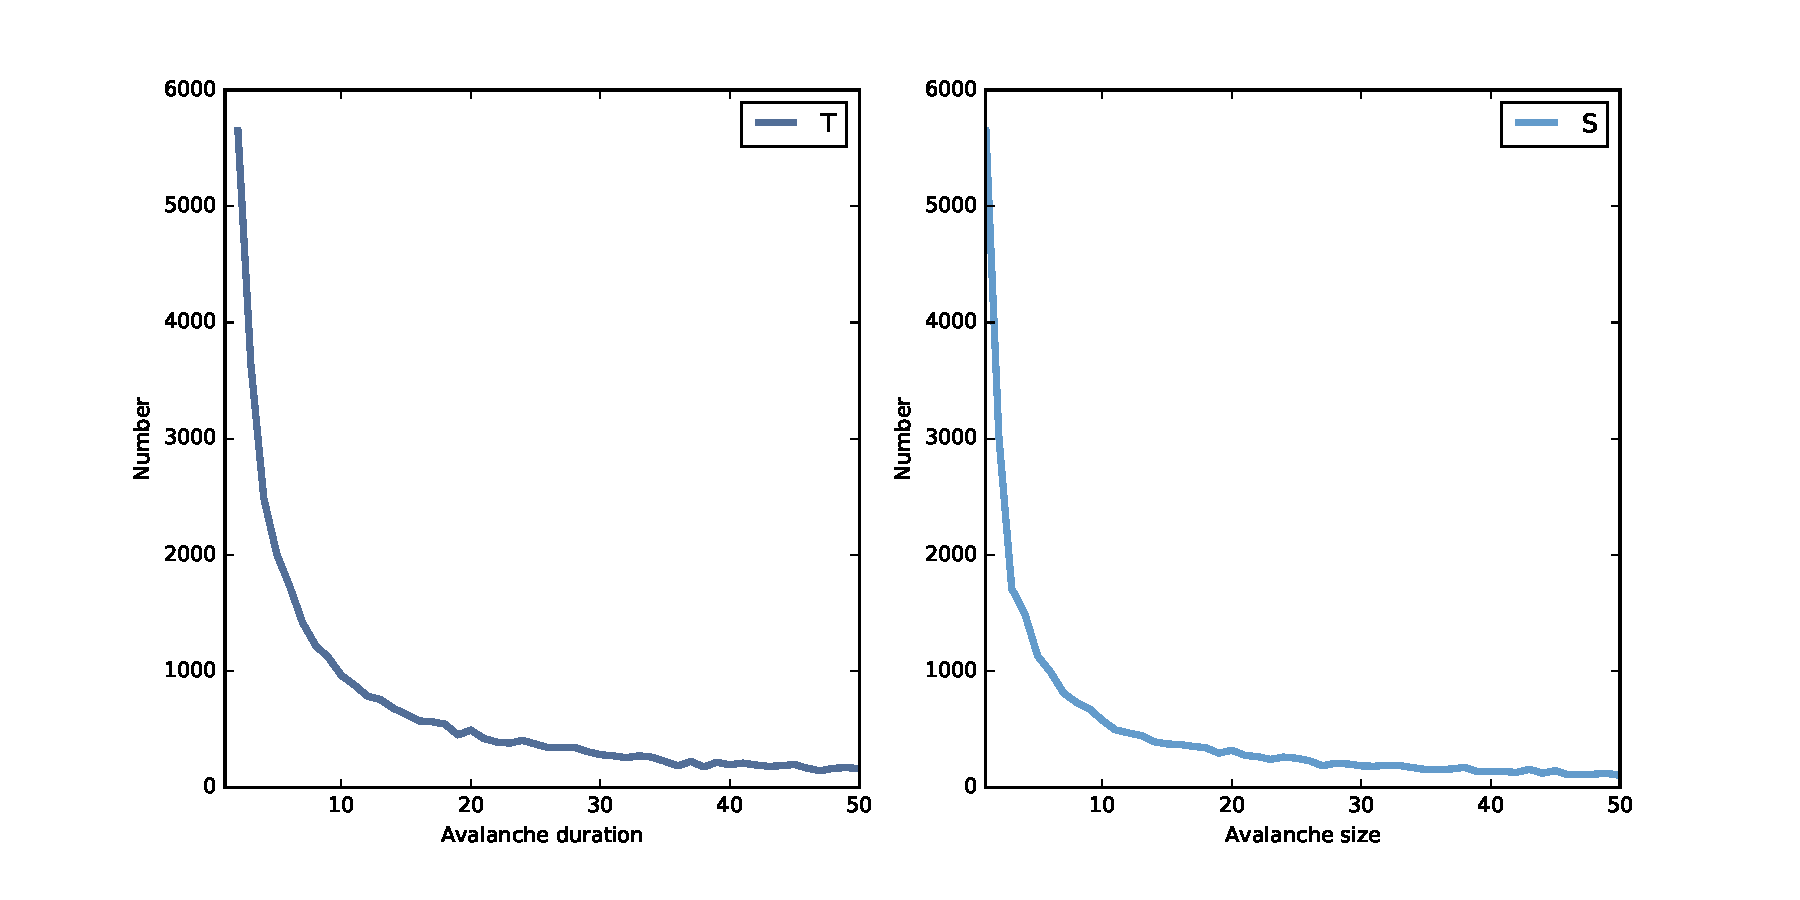
\includegraphics[height=3in]{figs/chap08-2.pdf}}
\caption{Distribution of avalanche duration (left) and size (right), linear scale.}
\label{chap08-2}
\end{figure}

\begin{figure}
\centerline{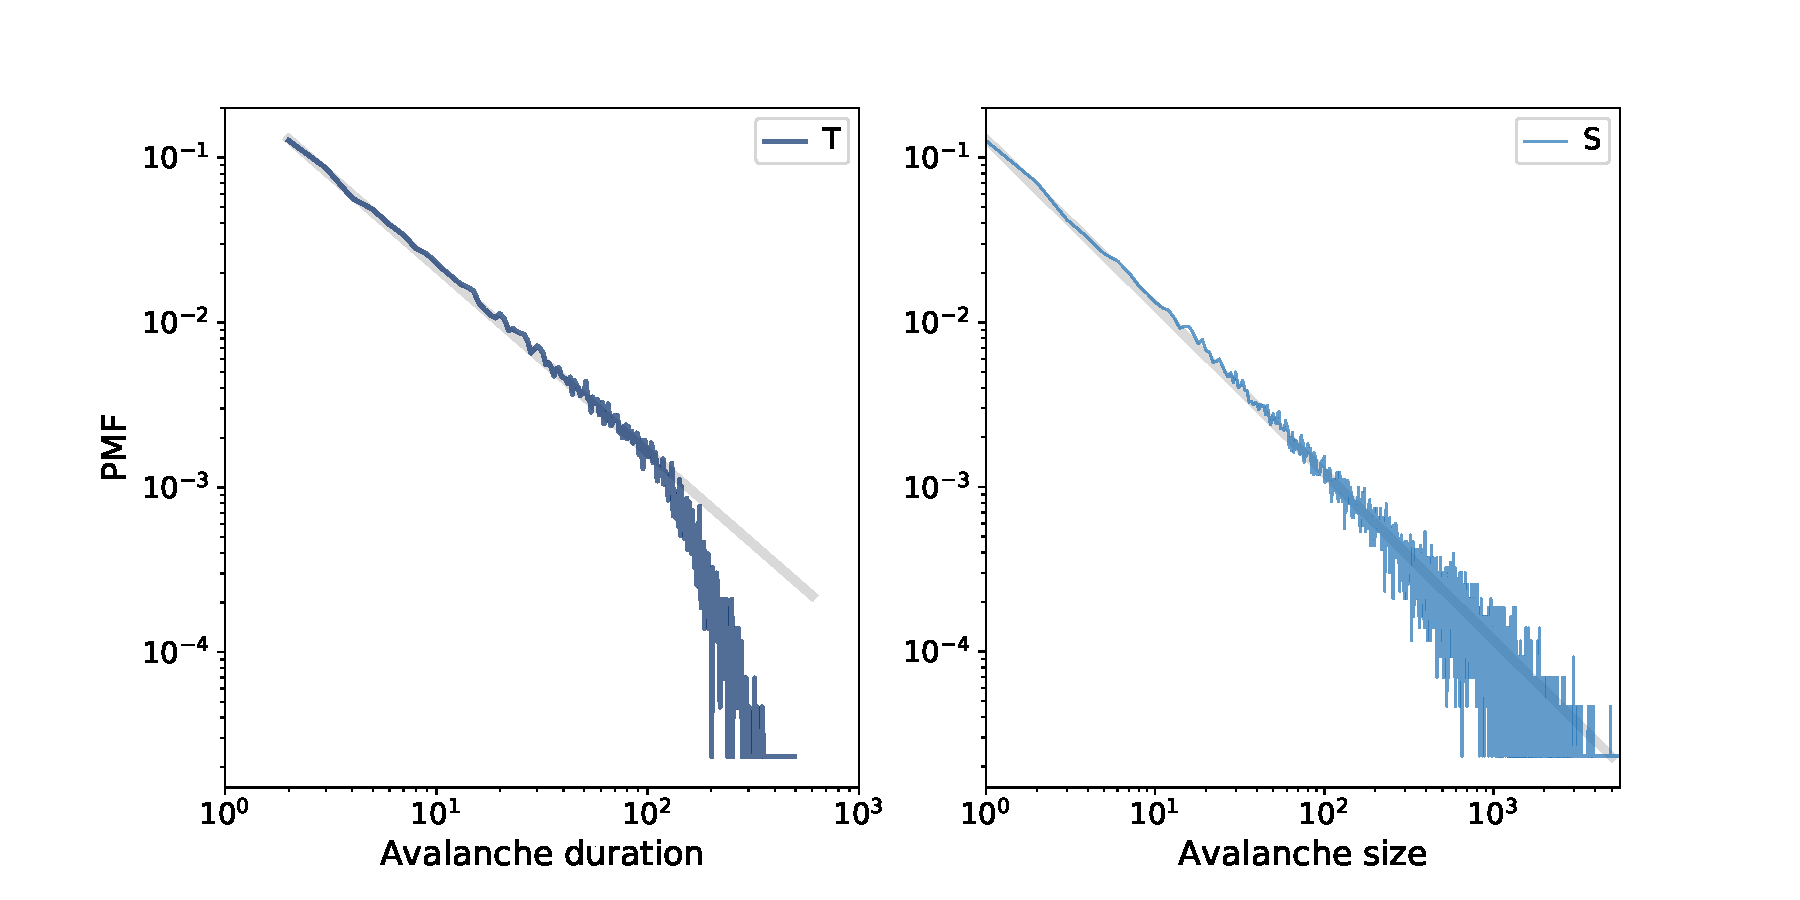
\includegraphics[height=3in]{figs/chap08-3.pdf}}
\caption{Distribution of avalanche duration (left) and size (right), log-log scale.}
\label{chap08-3}
\end{figure}

Figure~\ref{chap08-2} shows the results for values less than 50.
But as we saw in Section~\ref{heavytail}, we can get a clearer picture of
these distributions by plotting them on a log-log scale, as shown
in Figure~\ref{chap08-3}.

For values between 1 and 100, the distributions are nearly straight
on a log-log scale, which is indicative of a heavy tail.  The
gray lines in the figure have slope -1, which suggests that these
distributions follow a power law with parameter $\alpha=1$.

For values greater than 100, the distributions fall away more quickly
than the power law model, which means there are fewer very large
values than the model predicts.  One explanation is that this
effect is due to the finite size of the sand pile, so we might
expect larger piles to fit the power law better.

Another possibility,
which you can explore in one of the exercises at the end of this
chapter, is that these distributions do not strictly obey a power
law.  But even if they are not power-law distributions, they are
still heavy-tailed as we expect for a system in a critical state.


\section{Fractals}
\label{sandfrac}

Another property of critical systems is fractal geometry.  The
initial configuration in Figure~\ref{chap08-1} (left) resembles a fractal,
but you can't always tell by looking.
A more reliable way to identify a fractal is to estimate its
fractal dimension, as we saw in Section~\ref{fractals}
and Section~\ref{fracperc}.

I'll start by making a bigger sand pile, with \py{n=131} and initial
level \py{22}.

\begin{code}
pile3 = SandPile(n=131, level=22)
pile3.run()
\end{code}

By the way, it takes 28,379 steps for this pile to reach equilibrium,
with more than 200 million cells toppled.

To see the resulting pattern more clearly, I select cells with
levels 0, 1, 2, and 3, and plot them separately:

\begin{code}
def draw_four(viewer, vals=range(4)):
    thinkplot.preplot(rows=2, cols=2)
    a = viewer.viewee.array

    for i, val in enumerate(vals):
        thinkplot.subplot(i+1)
        viewer.draw_array(a==vals[i], vmax=1)
\end{code}

\py{draw_four} takes a \py{SandPileViewer} object, which is defined
in \py{Sand.py}.  The parameter \py{vals} is the list of values
we want to plot; the default values are 0, 1, 2, and 3.

Here's how it's used:

\begin{code}
viewer3 = SandPileViewer(pile3)
draw_four(viewer3)
\end{code}

\begin{figure}
\centerline{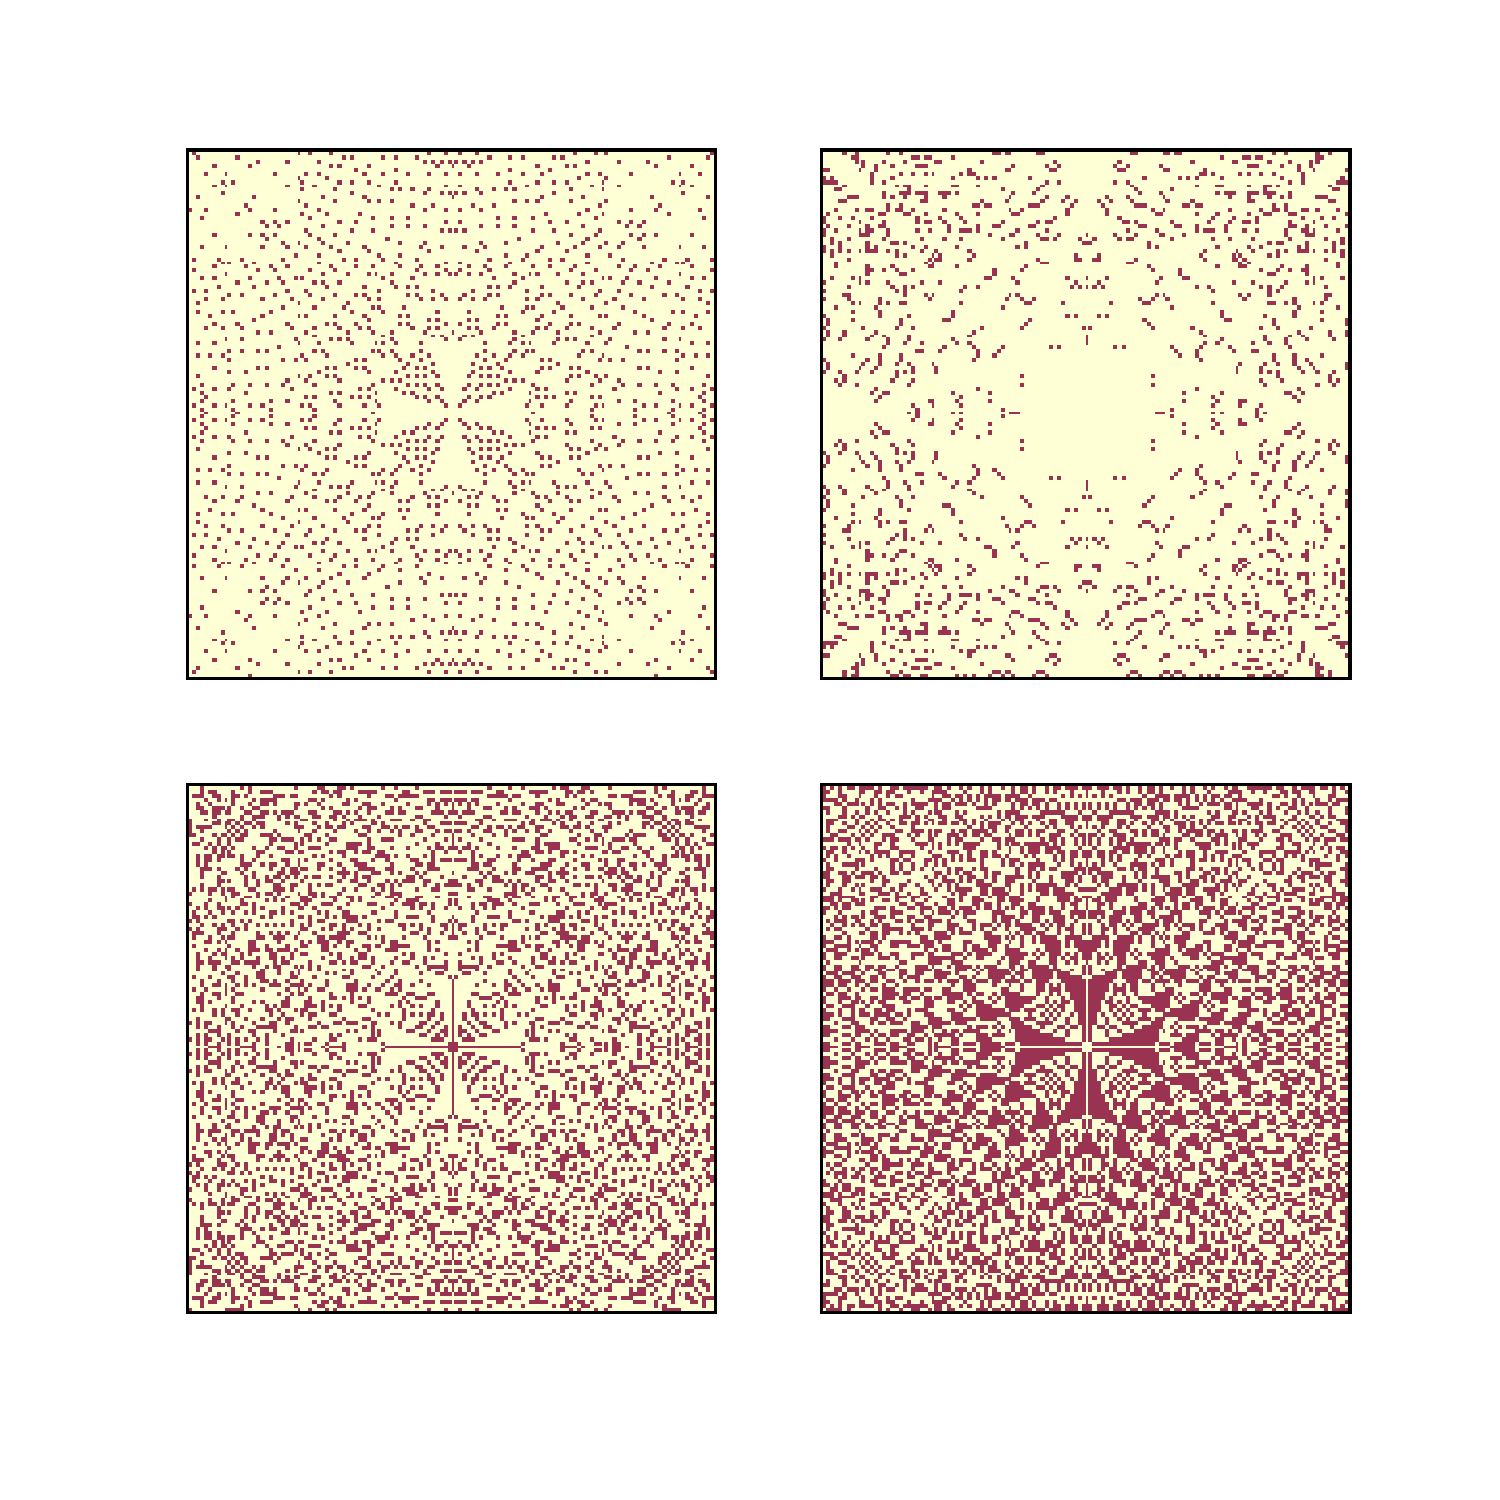
\includegraphics[height=3in]{figs/chap08-4.pdf}}
\caption{Sand pile model initial state, selecting cells with levels 0, 1, 2, and 3, top to bottom, left to right. }
\label{chap08-4}
\end{figure}

Figure~\ref{chap08-4} shows the results.  Now for each of
these patterns we can estimate the fractal dimension using
a {\bf box-counting algorithm}: we'll count the number of
cells in a small box at the center of the pile, and then see
how the number of cell increases as the box gets bigger.
Here's my implementation:

\begin{code}
def count_cells(a):
    n, m = a.shape
    end = min(n, m)

    res = []
    for i in range(1, end, 2):
        top = (n-i) // 2
        left = (m-i) // 2
        box = a[top:top+i, left:left+i]
        total = np.sum(box)
        res.append((i, i**2, total))

    return np.transpose(res)
\end{code}

The parameter, \py{a}, is a NumPy array of booleans or 0s and 1s.
The size of the box is initially 1.  Each time through the
loop, it increases by 2 until it reaches \py{end}, which is the
smaller of \py{n} and \py{m}.

Each time through the loop, \py{box} is a set of cells with width
and height \py{i}, centered in the array.  \py{total} is the number
of ``on'' cells in the box.

The result is a list of tuples, where each tuple contains
\py{i} and \py{i**2}, for purposes of comparison, and the number of
cells in the box.

Finally, we use \py{np.transpose} to make a NumPy array with 3
rows containing \py{i}, \py{i**2}, and \py{total}.

To estimate the fractal dimension, we extract the rows:

\begin{code}
steps, steps2, cells = res
\end{code}

Then we can plot the results:

\begin{code}
    thinkplot.plot(steps, steps2, linestyle='dashed')
    thinkplot.plot(steps, cells)
    thinkplot.plot(steps, steps, linestyle='dashed')
\end{code}

And use \py{linregress} to fit a line on a log-log scale.

\begin{code}
from scipy.stats import linregress

params = linregress(np.log(steps), np.log(cells))
slope = params[0]
\end{code}

\begin{figure}
\centerline{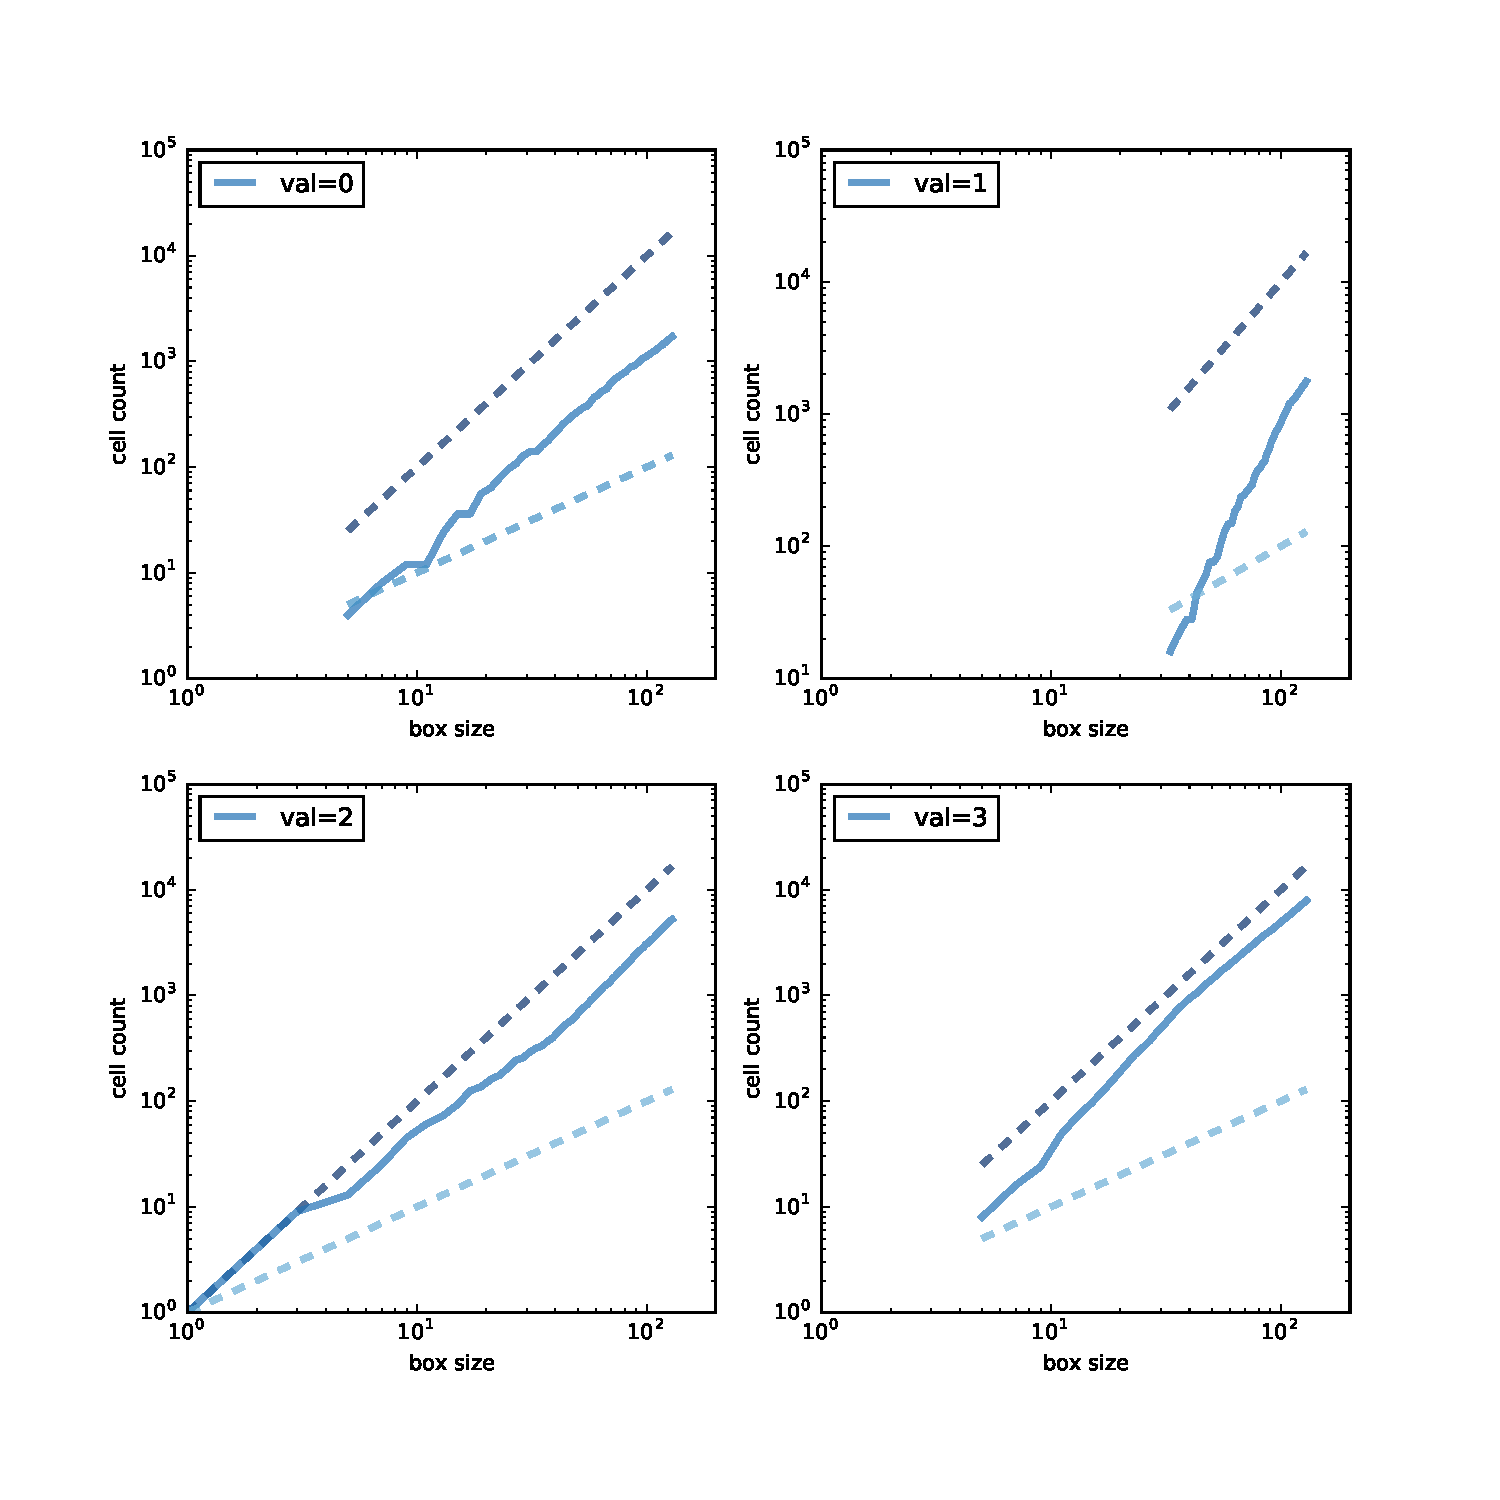
\includegraphics[height=4in]{figs/chap08-5.pdf}}
\caption{Box counts for cells with levels 0, 1, 2, and 3, compared to dashed lines with slopes 1 and 2.}
\label{chap08-5}
\end{figure}

Figure~\ref{chap08-5} shows the results.  Notice that only
\py{val=2} (lower left) starts from box size 1 because the center
cell has value 2; the other lines start at the first box size
that contains a nonzero cell count.

On a log-log scale, the cell counts form nearly straight lines,
which indicates that we are measuring fractal dimension over
a valid range of box sizes.

And the estimated fractal dimensions are:

\begin{code}
0  1.871
1  3.502
2  1.781
3  2.084
\end{code}

The fractal dimension for values 0, 1, and 2 seems to be clearly
non-integer, which indicates that the image is fractal.

Strictly, the fractal dimension for value 3 is indistinguishable from
2, but given the results for the other values, the apparent curvature
of the line, and the appearance of the pattern, it seems likely that
it is also fractal.

One of the exercises at the end of this chapter asks you to run
this analysis again with different values of \py{n} and \py{level} to
see if the estimated dimensions are consistent.


\section{Spectral Density}

The title of the original paper that presented the sand pile model
is ``Self-Organized Criticality: An Explanation of $1/f$ Noise''.
As the subtitle suggests, Bak, Tang and Wiesenfeld were trying to
explain why many natural and engineered systems exhibit $1/f$
noise, which is also known as ``flicker noise'' and ``pink noise''.

To understand pink noise, we have to take a detour to understand
signals, spectral analysis, and noise.

\begin{description}

\item[Signal:] A {\bf signal} is any quantity that varies in time.
  One example is sound, which is variation in air density.  In this
  section we'll explore how avalanche durations and sizes vary over
  time steps.

\item[Spectral analysis:] Any signal can be decomposed into a set of
  frequency components with different volume or power.  For example,
  the sound of a violin playing the A above middle C contains a
  dominant component at frequency 440 Hz, but it also contains less
  powerful components at 880 Hz, 1320 Hz, and other integer multiples
  of the fundamental.  {\bf Spectral analysis} is the process of
  finding the components that make up a signal and their powers,
  which is called its {\bf spectrum}.

\item[Noise:] In common use, ``noise'' is usually an unwanted sound,
  but in the context of signal processing, it is a signal that
  contains many frequency components.

\end{description}

There are many kinds of noise.  For example, ``white noise'' is a
signal that has components with equal power over a wide range of
frequencies.

Other kinds of noise have different relationships between frequency
and power.  In ``red noise'', the power at frequency $f$ is
$1/f^2$, which we can write like this:

\[ P(f) = 1/f^2 \]

We can generalize that by replacing the exponent $2$ with
a parameter $\beta$:

\[ P(f) = 1/f^\beta \]

When $\beta=0$, this equation describes white noise; when $\beta=2$ it
describes red noise.  When the parameter is near 1, we call the result
$1/f$ noise.  More generally, noise with any value between 0 and 2
is called ``pink'', because it's between white and red.

So how does this apply to the sand pile model?  Suppose that every time
a cell topples, it makes a sound.  If we recorded a sand pile model
while its running, what would it sound like?

As my implementation of \py{SandPile} runs, it records the number of
cells that topple during each time step, recording the results in
a list called \py{toppled_seq}.  For example, after running the model
in Section~\ref{heavysand}, we can extract the resulting signal:

\begin{code}
signal = pile2.toppled_seq
\end{code}

To compute the spectrum of a signal (again, that's the frequencies it
contains and their powers) we can use the Fast Fourier Transform
(FFT).

The only problem is that the spectrum of a noise signal tends to
be noisy.  However, we can smooth it out by breaking a long signal
into segments, computing the FFT of each segment, and then computing
the {\em average} power at each frequency.

One version of this algorithm is called ``Welch's method'' and
SciPy provides an implementation.  We can use it like this:

\begin{code}
from scipy.signal import welch

nperseg = 2048
freqs, spectrum = welch(signal, nperseg=nperseg, fs=nperseg)
\end{code}

\py{nperseg} is the length of the segments the signal is broken into.
With longer segments we get more frequency components,
but since there are fewer segments to average, the results are
noisier.

\py{fs} is the ``sampling frequency'', which is the number of data
points in the signal per unit of time.  By setting \py{fs=nperseg},
we get a range of frequencies from 0 to \py{nperseg/2}, but the
units of time in the model are arbitrary, so the frequencies
don't mean very much.

The return values, \py{freqs} and \py{powers}, are NumPy arrays containing
the frequencies of the components and their corresponding powers.

If the signal is pink noise, we expect

\[ P(f) = 1/f^\beta \]

Taking the log of both sides yields

\[ \log P(f) = -\beta \log f \]

So if we plot \py{powers} versus \py{freqs} on a log-log scale, we
expect a straight line with slope $-\beta$.

\begin{figure}
\centerline{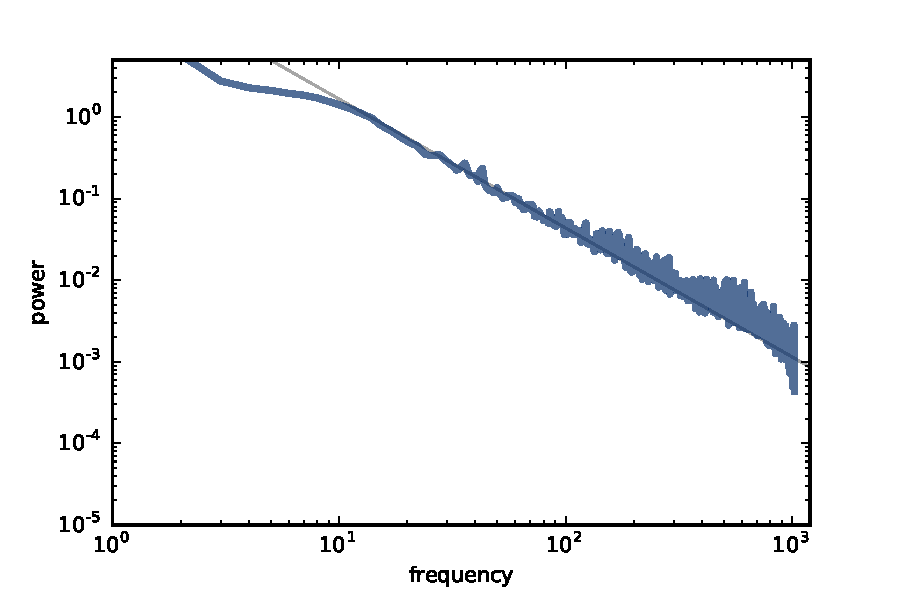
\includegraphics[height=3in]{figs/chap08-6.pdf}}
\caption{Power spectrum of the number of toppled cells over time, log-log scale.}
\label{chap08-6}
\end{figure}

Figure~\ref{chap08-6} shows the result.  For frequencies between
10 and 1000 (in arbitrary units), the spectrum falls on a straight
line.  The gray line has slope $-1.58$, which
corresponds to the parameter, $\beta=1.58$ reported by Bak,
Tang, and Wiesenfeld.

This result confirms that the sand pile model generates pink noise.


\section{Reductionism and Holism}
\label{model2}

The original paper by Bak, Tang and Wiesenfeld is one of
the most frequently-cited papers in the last few decades.
Other systems have been shown to be self-organized critical,
and the sand-pile model, in particular, has been studied
in detail.
\index{sand pile model}

As it turns out, the sand pile model is not a very good model of a
sand pile.  Sand is dense and not very sticky, so momentum has a
non-negligible effect on the behavior of avalanches.  As a result,
there are fewer very large and very small avalanches than the model
predicts, and the distribution might not be heavy-tailed.

Bak has suggested that this observation misses the point.
The sand pile model is not meant to be a realistic model of a sand
pile; it is meant to be a simple model for a broad category of
systems.

To understand this point, it is useful to think about two
kinds of models, {\bf reductionist} and {\bf holistic}.  A
reductionist model describes a system by describing its parts
and their interactions.  When a reductionist model is used
as an explanation, it depends on an analogy between the
components of the model and the components of the system.

\index{reductionist}
\index{holist}

For example, to explain why the ideal gas law holds, we can model the
molecules that make up a gas with point masses and model their
interactions as elastic collisions.  If you simulate or analyze this
model, you find that it obeys the ideal gas law.  This model is
satisfactory to the degree that molecules in a gas behave like
molecules in the model.  The analogy is between the parts of the
system and the parts of the model.

\index{analogy}

\begin{figure}
\centerline{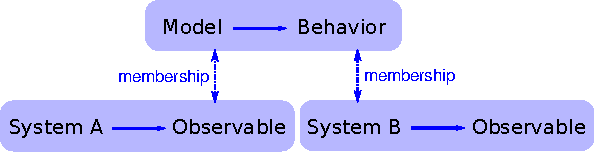
\includegraphics[width=5in]{figs/model2.pdf}}
\caption{The logical structure of a holistic model.\label{fig.model2}}
\end{figure}

Holistic models are more focused on similarities between systems and
less interested in analogous parts.  A holistic approach to modeling
often consists of two steps, not necessarily in this order:

\index{holistic model}

\begin{itemize}

\item Identify a kind of behavior that appears in a variety of
systems.

\item Find a simple model that demonstrates that behavior.

\end{itemize}

For example, in {\em The Selfish Gene}, Richard Dawkins suggests that
genetic evolution is just one example of an evolutionary system.  He
identifies the essential elements of the category---discrete
replicators, variability, and differential reproduction---and proposes
that any system with these elements displays similar
behavior, including complexity without design.

\index{Selfish Gene@{\em The Selfish Gene}}
\index{Dawkins, Richard}
\index{evolution}

As another example of an evolutionary system, he proposes ``memes'',
which are thoughts or behaviors that are replicated by transmission
from person to person\footnote{This use of ``meme'' is original to
  Dawkins, and predates the distantly-related use of the word on the
  Internet by about 20 years.}.  As memes compete for the resource of
human attention, they evolve in ways that are similar to genetic
evolution.

\index{meme}
\index{replicator}

Critics of the meme model have pointed out that
memes are a poor analogy for genes.  Memes differ from genes in many
obvious ways.  But Dawkins has argued that these differences are
beside the point because memes are not {\em supposed} to be analogous
to genes.  Rather, memes and genes are examples of the same
category: evolutionary systems.  The differences between them
emphasize the real point, which is that evolution is a general model
that applies to many seemingly disparate systems.  The logical
structure of this argument is shown in Figure~\ref{fig.model2}.

\index{gene}
\index{genetics}

Bak has made a similar argument that self-organized criticality is a
general model for a broad category of system:

\begin{quote}
Since these phenomena appear everywhere, they cannot depend on any
specific detail whatsoever...  If the physics of a large class of
problems is the same, this gives [the theorist] the option of selecting
the {\em simplest} possible [model] belonging to that class for detailed
study.\footnote{Bak, {\em How Nature Works}, Springer-Verlag 1996, page 43.}
\end{quote}

\index{Bak, Per}

Many natural systems demonstrate behaviors characteristic of critical
systems.  Bak's explanation for this prevalence is that these systems
are examples of the broad category of self-organized criticality.
There are two ways to support this argument.  One is to build
a realistic model of a particular system and show that the model
exhibits SOC.  The second is to show that SOC is a feature of many
diverse models, and to identify the essential characteristics
those models have in common.

The first approach, which I characterize as reductionist, can explain
the behavior of a particular system.  The second, holistic, approach,
explains the prevalence of criticality in natural systems.  They are
different models with different purposes.

\index{prevalence}

For reductionist models, realism is the primary virtue, and simplicity
is secondary.  For holistic models, it is the other way around.


\section{SOC, causation and prediction}

If a stock market index drops by a fraction of a percent in a
day, there is no need for an explanation.  But if it drops 10\%,
people want to know why.  Pundits
on television are willing to offer explanations, but the real
answer may be that there is no explanation.

\index{stock market}

Day-to-day variability in the stock market shows evidence of
criticality: the distribution of value changes is heavy-tailed
and the time series exhibits pink noise.
If the stock market is a critical system, we
should expect occasional large changes as part of the ordinary
behavior of the market.

The distribution of earthquake sizes is also heavy-tailed,
and there are simple models of the dynamics of geological faults
that might explain this behavior.  If these models are right,
they imply that large earthquakes are unexceptional; that is,
they do not require explanation any more than
small earthquakes do.

\index{earthquake}
\index{prediction}
\index{causation}

Similarly, Charles Perrow has suggested that failures in large
engineered systems, like nuclear power plants, are like avalanches
in the sand pile model.  Most failures are small, isolated and
harmless, but occasionally a coincidence of bad fortune yields a
catastrophe.  When big accidents occur, investigators go looking for
the cause, but if Perrow's ``normal accident theory'' is correct,
there may be no special cause of large failures.

\index{normal accident theory}
\index{Perrow, Charles}

These conclusions are not comforting.  Among other things, they
imply that large earthquakes and some kinds of accidents are
fundamentally unpredictable.  It is impossible to look at the
state of a critical system and say whether a large avalanche
is ``due''.  If the system is in a critical state, then a large
avalanche is always possible.  It just depends on the
next grain of sand.

In a sand pile model, what is the cause of a large avalanche?
Philosophers sometimes distinguish the {\bf proximate} cause, which is
most immediately responsible, from the {\bf ultimate} cause, which is,
for whatever reason, considered the true cause.

\index{proximate cause}
\index{ultimate cause}

In the sand pile model, the proximate cause of an avalanche is
a grain of sand, but the grain that causes a large avalanche
is identical to every other grain, so it offers no special explanation.
The ultimate cause of a large avalanche is the structure and
dynamics of the systems as a whole: large avalanches occur because
they are a property of the system.

Many social phenomena, including wars, revolutions, epidemics,
inventions and terrorist attacks, are characterized by heavy-tailed
distributions.  If the reason for these distributions is that
social systems are critical, that suggests that major historical
events may be fundamentally unpredictable and unexplainable.

\index{heavy-tailed distributions}


\section{Exercises}


\begin{exercise}


The code for this chapter is in the Jupyter notebook {\tt chap08.ipynb}
in the repository for this book.  Open this notebook, read the code,
and run the cells.  You can use this notebook to work on the
exercises in this chapter.  My solutions are in {\tt chap08soln.ipynb}.

\end{exercise}


\begin{exercise}

To test whether the distributions of \py{T} and \py{S} are
heavy-tailed, we plotted their histograms on a log-log scale, which is
what Bak, Tang and Wiesenfeld show in their paper.  But as we saw in
Section~\ref{cdf}, this visualization can obscure the shape of the
distribution.  Using the same data, make a plot that shows the
cumulative distributions (CDFs) of \py{S} and \py{T}.  What can you
say about their shape?  Do they follow a power law?  Are they heavy
tailed?

You might find it helpful to plot the CDFs on a log-x scale and on a
log-log scale.

\end{exercise}

\begin{exercise}

In Section~\ref{sandfrac} we showed that the initial configuration of
the sand pile model produces fractal patterns.  But after we drop a
large number of random grains, the patterns look more random.

Starting with the example in Section~\ref{sandfrac}, run the sand pile
model for a while and then compute fractal dimensions for each of the
4 levels.  Is the sand pile model fractal in steady state?

\end{exercise}

\begin{exercise}

Another version of the sand pile model, called the ``single source''
model, starts from a different initial condition: instead of all cells
at the same level, all cells are set to 0 except the center cell,
which is set to a large value.  Write a function that creates a
\py{SandPile} object, sets up the single source initial condition, and
runs until the pile reaches equilibrium.  Does the result appear to be
fractal?

You can read more about this version of the sand pile model at
\url{http://math.cmu.edu/~wes/sandgallery.html}.

\end{exercise}


\begin{exercise}

In a 1989 paper, Bak, Chen and Creutz suggest that the Game of Life is
an SOC system.\footnote{``Self-organized criticality in the Game of
  Life'', available from
  \url{http://www.nature.com/nature/journal/v342/n6251/abs/342780a0.html}.}

\index{Game of Life}
\index{self-organized criticality}

To replicate their tests, run the GoL CA until it stabilizes,
then choose a random cell and flip it.  Run the CA until
it stabilizes again, keeping track of \py{T}, the number
of time steps it takes, and \py{S}, the number of cells affected.
Repeat for a large number of trials and plot the distributions
of \py{T} and \py{S}.  Also, record the number of cells that change
state during each time step and see if the resulting time series
resembles pink noise.

\end{exercise}


\begin{exercise}

In {\em The Fractal Geometry of Nature}, Benoit Mandelbrot proposes
what he calls a ``heretical'' explanation for the prevalence of
heavy-tailed distributions in natural systems.  It may not
be, as Bak suggests, that many systems can generate this behavior in
isolation.  Instead there may be only a few, but there may be
interactions between systems that cause the behavior to propagate.

\index{Mandelbrot, Benoit}
\index{heavy-tailed distribution}

To support this argument, Mandelbrot points out:

\begin{itemize}

\item The distribution of observed data is often ``the joint
  effect of a fixed underlying {\em true distribution} and a highly
  variable {\em filter}.''

\item Heavy-tailed distributions are robust to filtering; that is,
  ``a wide variety of filters leave their asymptotic behavior
  unchanged.''

\end{itemize}

What do you think of this argument?  Would you characterize
it as reductionist or holist?

\end{exercise}


\begin{exercise}

Read about the ``Great Man'' theory of history at
\url{http://en.wikipedia.org/wiki/Great_man_theory}.  What implication
does self-organized criticality have for this theory?

\index{Great Man theory}
\end{exercise}



\chapter{Agent-based models}
\label{agent-based}

The models we have seen so far might be characterized as ``rule-based''
in the sense that they involve systems governed by simple rules.  In this
and the following chapters, we explore {\bf agent-based models}.

\index{agent-based model}

Agent-based models include {\bf agents} that are
intended to model people and other entities that gather
information about the world, make decisions, and take actions.

The agents are usually situated in space or in a network, and
interact with each other locally.  They usually have imperfect,
incomplete information about the world.

Often there are differences among agents, unlike previous models where
all components are identical.  And agent-based models often include
randomness, either among the agents or in the world.

Since the 1970s, agent-based modeling has become an important tool in
economics and other social sciences, and in some natural sciences.

Agent-based models are useful for modeling the dynamics of systems
that are not in equilibrium (although they are also used to study
equilibrium).  And they are particularly useful for understanding
relationships between individual decisions and system behavior.

The code for this chapter is in \py{chap09.ipynb}, which is a
Jupyter notebook in the repository for this book.  For more information
about working with this code, see Section~\ref{code}.


\section{Schelling's Model}

In 1971 Thomas Schelling published ``Dynamic Models of Segregation'',
which proposes a simple model of racial segregation.  The Schelling
model of the world is a grid; each cell represents a house.  The
houses are occupied by two kinds of agents,
labeled red and blue, in roughly equal numbers.  About 10\% of the
houses are empty.

\index{Schelling, Thomas}

At any point in time, an agent might be happy or unhappy, depending
on the other agents in the neighborhood, where the
``neighborhood" of each house is the set of eight adjacent cells.
In one version of the model, agents are happy if they have at least
two neighbors like themselves, and unhappy if they have one or zero.

\index{agent-based model}

The simulation proceeds by choosing an agent at random and checking
to see whether they are happy.  If so, nothing happens; if not,
the agent chooses one of the unoccupied cells at random and moves.

You might not be surprised to hear that this model leads to some
segregation, but you might be surprised by the degree.  Fairly
quickly, clusters of similar agents appear.  The clusters
grow and coalesce over time until there are a small number
of large clusters and most agents live in homogeneous
neighborhoods.

\index{segregation}

If you did not know the process and only saw the result, you might
assume that the agents were racist, but in fact all of them
would be perfectly happy in a mixed neighborhood.  Since they prefer
not to be greatly outnumbered, they might be considered xenophobic at
worst.  Of course, these agents are a wild simplification of real
people, so it may not be appropriate to apply these descriptions at
all.

\index{racism}
\index{xenophobia}

Racism is a complex human problem; it is hard to imagine that such a
simple model could shed light on it.  But in fact it provides a strong
argument about the relationship between a system and its parts: if you
observe segregation in a real city, you cannot conclude that
individual racism is the immediate cause, or even that the people in
the city are racists.

\index{causation}

Of course, we have to keep in mind the limitations of this argument:
Schelling's model demonstrates a possible cause of segregation, but
says nothing about actual causes.


\section{Implementation of Schelling's model}

To implement Schelling's model, I wrote yet another class that
inherits from \py{Cell2D}:

\begin{code}
class Schelling(Cell2D):

    def __init__(self, n, m=None, p=0.5):
        self.p = p
        m = n if m is None else m
        choices = [0, 1, 2]
        probs = [0.1, 0.45, 0.45]
        self.array = np.random.choice(choices, (n, m), p=probs)
\end{code}

The parameters \py{n} and \py{m} are the dimensions of the grid,
and \py{p} is the threshold on the fraction of similar neighbors.
For example, if \py{p=0.5}, an agent will be unhappy if fewer
than 50\% of their neighbors are the same color.

\py{array} is a NumPy array where each cell is 0 if empty, 1 if
occupied by a red agent, and 2 if occupied by a blue agent.
Initially 10\% of the cells are empty, 45\% red, and 45\% blue.

The \py{step} function for Schelling's model is substantially more
complicated than previous step functions.  If you are not
interested in the details, you can skip to the next section.
But if you stick around, you might pick up some NumPy tips.

First, I'll make logical arrays indicating which cells are
red, blue, and occupied:

\begin{code}
        a = self.array
        red = a==1
        blue = a==2
        occupied = a!=0
\end{code}

I'll use \py{np.correlate2d} to count, for each cell,
the number of neighboring cells that are red and the number
that are occupied.

\begin{code}
    options = dict(mode='same', boundary='wrap')

    kernel = np.array([[1, 1, 1],
                       [1, 0, 1],
                       [1, 1, 1]], dtype=np.int8)

    num_red = correlate2d(red, kernel, **options)
    num_neighbors = correlate2d(occupied, kernel, **options)
\end{code}

%TODO: Update this code.

Now for each cell we can compute the fraction of neighbors
that are red and the fraction that are the same color:

\begin{code}
    frac_red = num_red / num_neighbors
    frac_blue = 1 - frac_red
    frac_same = np.where(red, frac_red, frac_blue)
\end{code}

\py{frac_red} is just the ratio of \py{num_red} and \py{num_neighbors},
and \py{frac_blue} is the complement of \py{frac_red}.

\py{frac_same} is a little bit more complicated.  The function
\py{np.where} is like an element-wise \py{if} expression.  The
first parameter is a condition that selects elements from
the second or third parameter.

\index{np.where}

In this case, wherever \py{red} is \py{True}, \py{frac_same} gets
the corresponding element of \py{frac_red}.  Where \py{red} is
\py{False}, \py{frac_same} gets the corresponding element of \py{frac_blue}.

Now we can identify the locations of the unhappy agents:

\begin{code}
    unhappy_locs = locs_where(occupied & (frac_same < self.p))
\end{code}

The result, \py{unhappy_locs}, is a NumPy array where each row is
the coordinates of an occupied cell where \py{frac_same} is below
the threshold \py{p}.

\py{locs_where} is a wrapper function for \py{np.nonzero}:

\begin{code}
def locs_where(condition):
    return np.transpose(np.nonzero(condition))
\end{code}

\py{np.nonzero} takes an array and returns the coordinates of
all non-zero cells, but the results are in the form of
two tuples.  \py{np.transpose} converts the results to a more
useful form, an array where each row is a coordinate pair.

Similarly, \py{empty_locs} is an array that contains the coordinates
of the empty cells, shuffled:

\begin{code}
    empty_locs = locs_where(a==0)
\end{code}

Now we get to the core of the simulation.  We loop through the
unhappy agents and move them:

\begin{code}
    for source in unhappy_locs:
        i = np.random.randint(len(empty_locs))
        dest = tuple(empty_locs[i])
        a[dest] = a[tuple(source)]
        a[tuple(source)] = 0
        empty_locs[i] = source
\end{code}

\py{i} is an index used to choose a random empty cell.

\py{dest} is a tuple containing the coordinates of the empty cell.

In order to move an agent, we copy the value from \py{source} to
\py{dest}, and then set the value of \py{source} to 0 (since it is now
empty).

Finally, we replace the entry in \py{empty_locs} with \py{source}, so the
cell that just became empty can be chosen by the next agent.


\section{Segregation}

\begin{figure}
\centerline{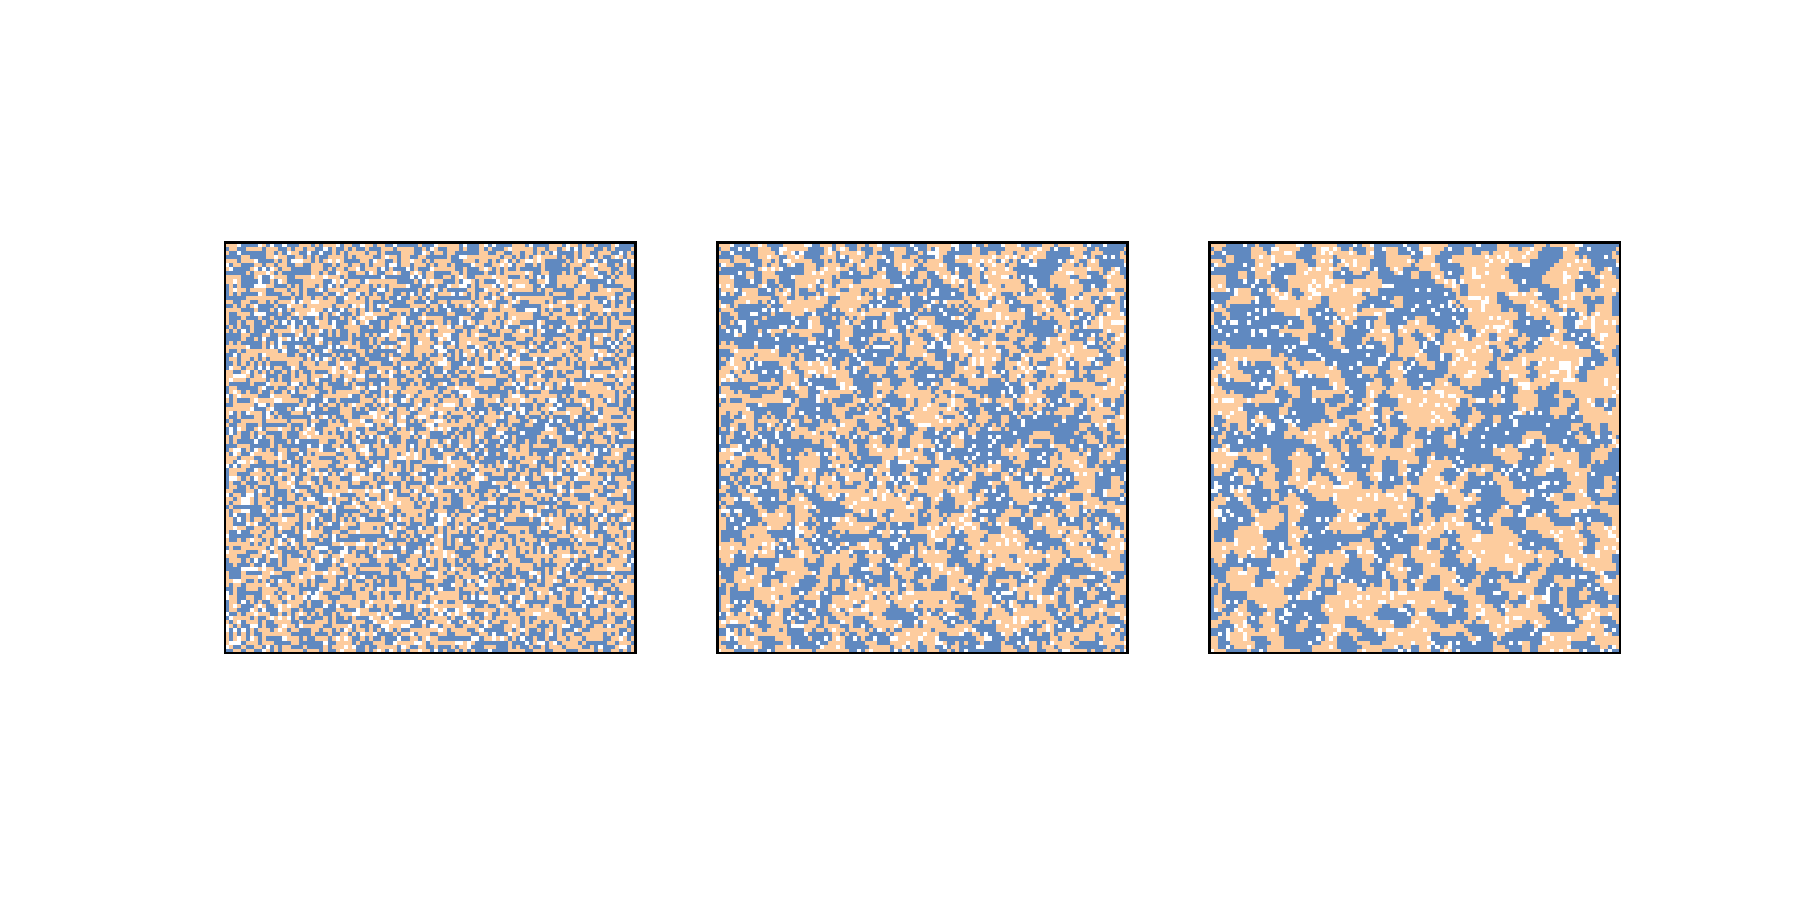
\includegraphics[height=3in]{figs/chap09-1.pdf}}
\caption{Schelling's segregation model with \py{n=100}, initial
condition (left), after 2 steps (middle) and after 10 steps (right).}
\label{chap09-1}
\end{figure}

Now let's see what happens when we run the model.  I'll start
with \py{n=100} and \py{p=0.3}, and run for 10 steps.

\begin{code}
grid = Schelling(n=100, p=0.3)
for i in range(10):
    grid.step()
\end{code}

Figure~\ref{chap09-1} shows the initial configuration (left),
the state of the simulation after 2 steps (middle) and after 10
steps (right).

Clusters form quickly, with red and blue agents moving into
segregated clusters separated by boundaries of empty cells.

For each configuration, we can compute the degree of segregation,
which is the fraction of neighbors who are the same color, averaged
across cells:

\begin{code}
    np.sum(frac_same) / np.sum(occupied)
\end{code}

In Figure~\ref{chap09-1}, the degree average fraction of similar
neighbors is 55\% in the initial configuration, 71\% after two
steps, and 80\% after 10 steps!

Remember that when \py{p=0.3} the agents would be happy if 3 of 8
neighbors were their own color, but they end up living in
neighborhood where 6 or 7 of their neighbors are their own color,
typically.


\begin{figure}
\centerline{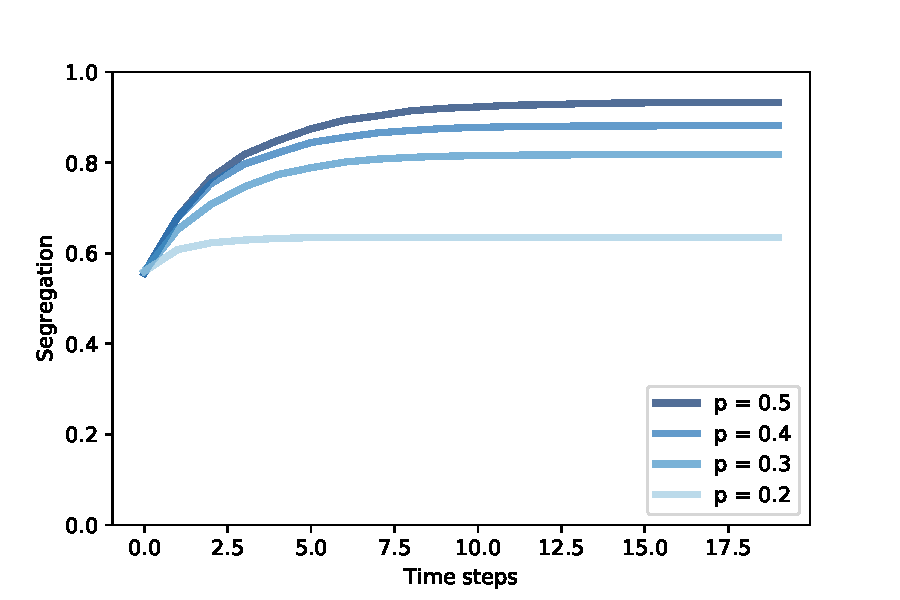
\includegraphics[height=3in]{figs/chap09-2.pdf}}
\caption{Degree of segregation in Schelling's model, over time,
for a range of \py{p}.}
\label{chap09-2}
\end{figure}

Figure~\ref{chap09-2} shows how the degree of segregation increases
and where it levels off for several values of \py{p}.  When \py{p=0.4},
the degree of segregation in steady state is about 88\%, and a majority
of agents have no neighbors with a different color.

These results are surprising to many people, and they make a striking
example of the complex and unpredictable relationship between
individual decisions and system behavior.


\section{Sugarscape}

% cjw: I think Epstein and Axtell use lower case for the second s.
% I've replaced all references except in code (\py{SugarScape}),
% where I think it's fine (or at least consistent with the notebooks,
% which I haven't looked at).

In 1996 Joshua Epstein and Robert Axtell proposed Sugarscape, an
agent-based model of an ``artificial society'' intended to support
experiments related to economics and other social sciences.

Sugarscape is a versatile model that has been adapted for a wide
variety of topics.  As examples, I will replicate the
first few experiments from Epstein and Axtell's book, {\it Growing
Artificial Societies}.

In its simplest form, Sugarscape is a model of a simple economy where
agents move around on a 2D grid, harvesting and accumulating ``sugar'',
which represents economic wealth.  Some parts of the grid produce more
sugar than others, and some agents are better at finding it than
others.

This version of Sugarscape is often used to explore and explain the
distribution of wealth, in particular the tendency toward inequality.

In the Sugarscape grid, each cell has a capacity, which is the maximum
amount of sugar it can hold.  In the original configuration, there
are two high-sugar regions, with capacity 4, surrounding by concentric
rings with capacities 3, 2, and 1.

\begin{figure}
\centerline{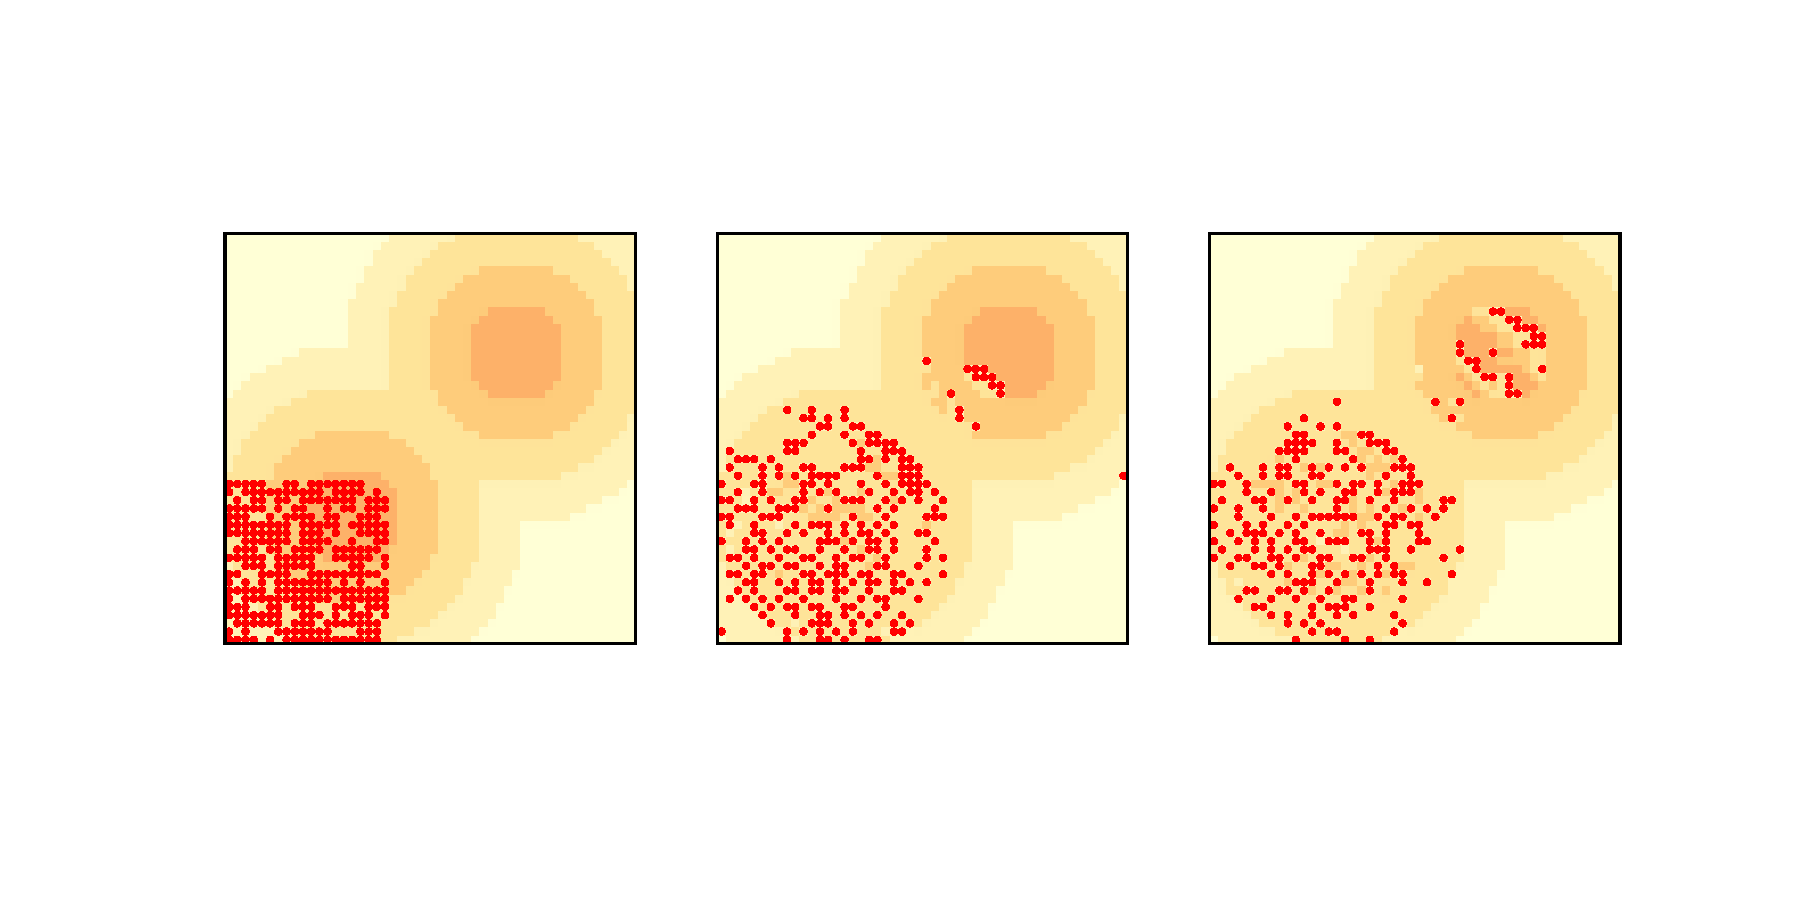
\includegraphics[height=3in]{figs/chap09-3.pdf}}
\caption{Replication of the original Sugarscape model: initial
configuration (left), after 2 steps (middle) and 100 steps (right).}
\label{chap09-3}
\end{figure}

Figure~\ref{chap09-3} (left) shows the initial configuration, with the darkest
areas indicating cells with the highest capacity, and small circles
representing the agents.

Initially there are 400 agents placed at random locations.  Each
agent has three randomly-chosen attributes:

\begin{description}

\item[Sugar:] Each agent starts with an endowment of sugar chosen
from a uniform distribution between 5 and 25 units.

\item[Metabolism:] Each agent has some amount of sugar they must
consume per time step, chosen uniformly between 1 and 4.

\item[Vision:] Each agent can ``see'' the amount
of sugar in nearby cells and move to the cell with the most, but
some agents can see farther than others.  The distance agents
see is chosen uniformly between 1 and 6.

\end{description}

During each time step, agents move one at a time in a random order.
Each agent follows these rules:

\begin{itemize}

\item The agent surveys \py{k} cells in each of the 4 compass directions,
where \py{k} is the range of the agent's vision.

\item It chooses the unoccupied cell with the most sugar.  In case
of a tie, it chooses the closer cell; among cells at the same
distance, it chooses randomly.

\item The agent moves to the selected cell and harvests the sugar,
adding the harvest to its accumulated wealth and leaving the cell
empty.

\item The agent consumes some part of its wealth, depending on its
metabolism.  If the resulting total is negative, the agent ``starves''
and is removed.

\end{itemize}

After all agents have executed these steps, the cells grow back
some sugar, typically 1 unit, but the total sugar in each cell is
bounded by its capacity.

Figure~\ref{chap09-3} (middle) shows the state of the model after two
steps.  Most agents are moving toward the areas with the most sugar.
Agents with high vision also move the fastest; agents with low vision
tend to get stuck on the plateaus, wandering randomly until they get
close enough to see the next level.

Agents born in the areas with the least sugar are likely to starve
unless they also have high vision and a high initial endowment.

Within the high-sugar areas, agents compete with each other to
find and harvest sugar as it grows back.  Agents with high metabolism
or low vision are the most likely to starve.

When sugar grows back at 1 unit per time step, there is not enough
sugar to sustain the 400 agents we started with.  The population
drops quickly at first, then more slowly, and levels off around 250.

Figure~\ref{chap09-3} (right) shows the state of the model after 100
time steps, with about 250 agents.  The agents who survive tend to
be the lucky ones, born with high vision and/or low metabolism.
Having survived to this point, they are likely to survive forever,
accumulating unbounded stockpiles of sugar.


\section{Wealth inequality}

In its current form, Sugarscape models a simple ecology, and could
be used to explore the relationship between the parameters of the
model, like the growth rate and the attributes of the agents, and
the carrying capacity of the system (the number of agents that
survive in steady state).  And it models a form of natural selection,
where agents with higher ``fitness'' are more likely to survive.

The model also demonstrates a kind of wealth inequality, with some
agents accumulating sugar faster than others.  But it would be hard
to say anything specific about the distribution of wealth because it
is not ``stationary''; that is, the distribution changes over time and
does not reach a steady state.

However, if we give the agents finite lifespans, the model produces
a stationary distribution of wealth.  And then we can run experiments to
see what effect the parameters and rules have on this distribution.

In this version of the model, agents have an age that gets incremented
each time step, and a random lifespan that is uniform from 60 to 100.
If an agent's age exceeds its lifespan, it dies.

When an agent dies, from starvation or old age, it is replaced by
a new agent with random attributes, so the total population is
constant.

\begin{figure}
\centerline{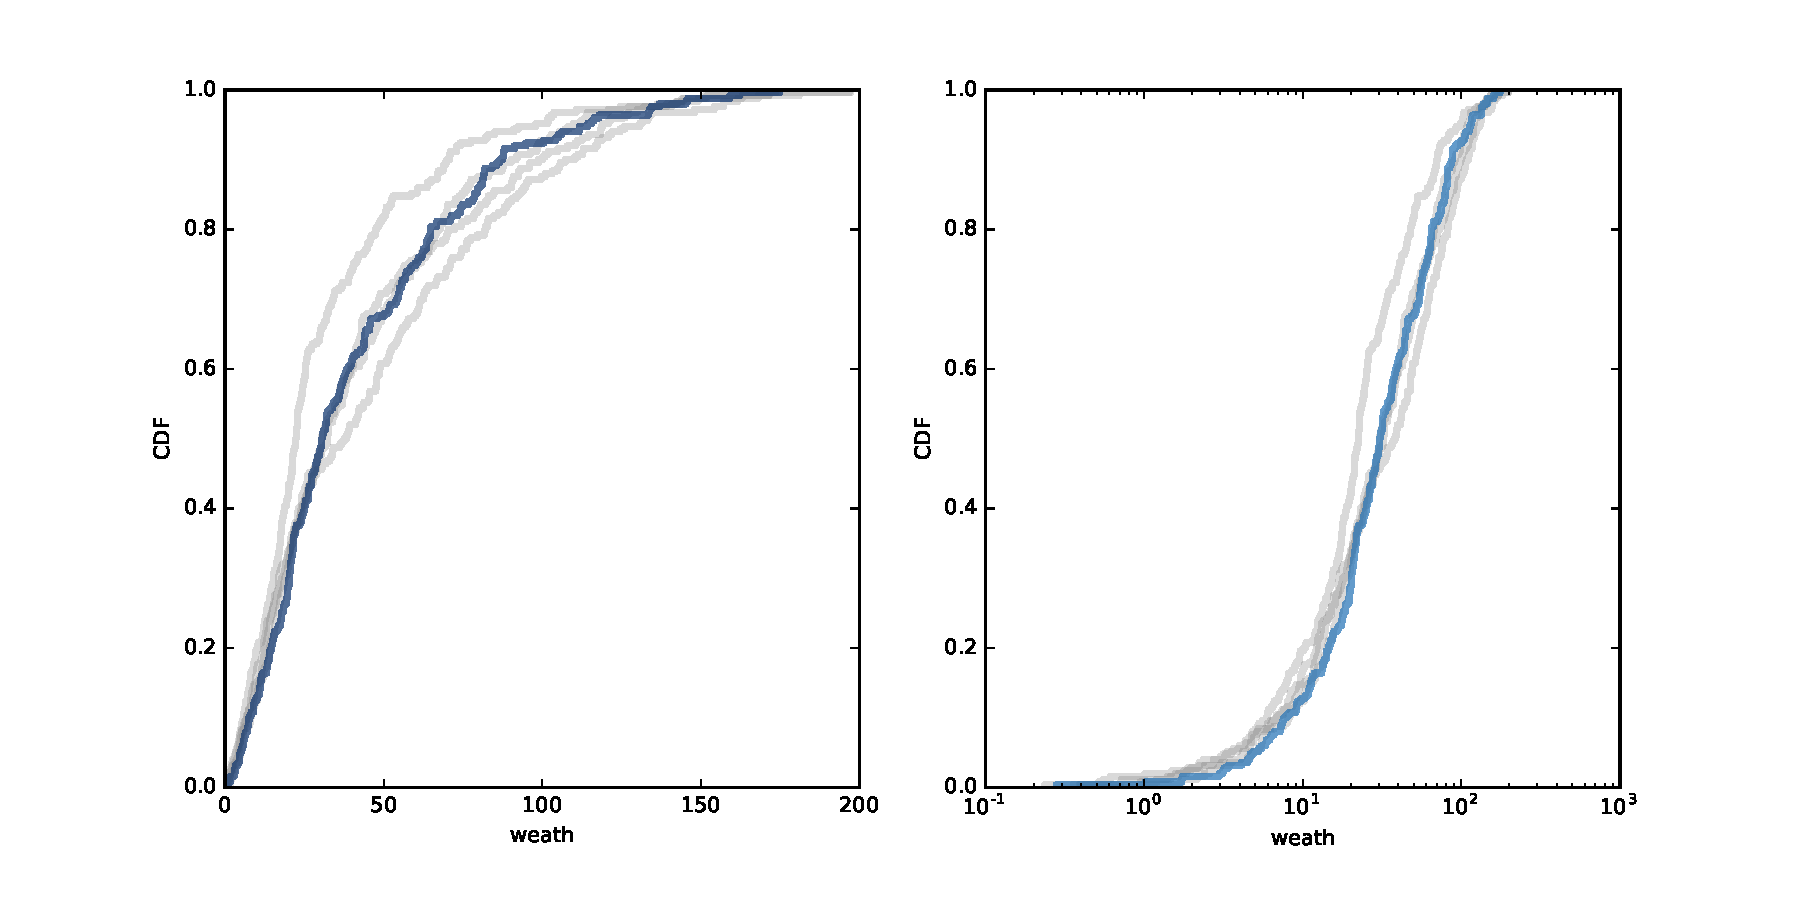
\includegraphics[height=3in]{figs/chap09-4.pdf}}
\caption{Distribution of sugar (wealth) after 100, 200, 300, and
400 steps (gray lines) and 500 steps (dark line).  Linear scale (left)
and log-x scale (right). }
\label{chap09-4}
\end{figure}

Starting with 250 agents, which is close to carrying capacity, I ran
the model for 500 steps.  After each 100 steps, I plot the distribution
of sugar accumulated by the agents.  Figure~\ref{chap09-4} shows the
results on a linear scale (left) and a log-x scale (right).

After about 200 steps (which is twice the longest lifespan) the
distribution doesn't change much.  And it is skewed to the right.

Most agents have little accumulated wealth: the 25th percentile is
about 10 and the median is about 20.  But a few agents have accumulated
much more: the 75th percentile is about 40, and the highest value is
more than 150.

On a log scale the shape of the distribution resembles a Gaussian or
normal distribution, although the right tail is truncated.  If it were
actually normal on a log scale, the distribution would be lognormal,
which is a heavy-tailed distribution.  And in fact, the distribution
of wealth in practically every country, and in the world, is a
heavy-tailed distribution.

It would be too much to claim that Sugarscape explains why wealth
distributions are heavy-tailed, but the prevalence of inequality in
variations of Sugarscape suggests that inequality is
characteristic of many economies, even very simple ones.
And experiments with rules that model taxation and other income
transfers suggest that it is not easy to avoid or mitigate.



\section{Implementing Sugarscape}

Sugarscape is more complicated than the previous models, so I won't
present the entire implementation here.  I will outline the
structure of the code and you can see the details in the Jupyter notebook
for this chapter, {\tt chap09.ipynb}, which is in the repository
for this book.  And if you are not interested in the details, you
can skip to the next section.

Here is the \py{Agent} class with the \py{step} method:

\begin{code}
class Agent:

    def step(self, env):
        self.loc = env.look_around(self.loc, self.vision)
        self.sugar += env.harvest(self.loc) - self.metabolism
        self.age += 1
\end{code}

During each step, the agent moves, harvests sugar, and increments
\py{age}.

The parameter \py{env} is a reference to the environment, which
is a \py{Sugarscape} object.  It provides methods \py{look_around} and
\py{harvest}:

\begin{itemize}

\item \py{look_around} takes the location of the agent, which is a
tuple of coordinates, and the range of the agent's vision, which is
an integer.  It returns the agent's new location, which is the
visible cell with the most sugar.

\item \py{harvest} takes the (new) location of the agent, and removes and
returns the sugar at that location.

\end{itemize}

And here's the \py{Sugarscape} class and its \py{step} method
(without replacement):

\begin{code}
class Sugarscape(Cell2D):

    def step(self):

        # loop through the agents in random order
        random_order = np.random.permutation(self.agents)
        for agent in random_order:

            # mark the current cell unoccupied
            self.occupied.remove(agent.loc)

            # execute one step
            agent.step(self)

            # if the agent is dead, remove from the list
            if agent.is_starving():
                self.agents.remove(agent)
            else:
                # otherwise mark its cell occupied
                self.occupied.add(agent.loc)

        # grow back some sugar
        self.grow()
        return len(self.agents)
\end{code}

\py{Sugarscape} inherits from \py{Cell2D}, so it is similar to the
other grid-based models we've seen.

The attributes include \py{agents}, which is a list of \py{Agent}
objects, and \py{occupied}, which is a set of tuples, where each
tuples contains the coordinates of a cell occupied by an agent.

During each step, the \py{Sugarscape} loops through the agents in
random order.  It invokes \py{step} on each agent and then checks whether
it is dead.  After all agents have moved, some of the sugar grows back.

If you are interested in learning more about NumPy, you might want
to look more closely at \py{make_visible_locs}, which builds an
array where each row contains the coordinates of a cell visible
to an agent, sorted by distance but with cells at the same distance
appearing in random order.

And you might want to look at \py{Sugarscape.make_capacity}, which
initializes the capacity of the cells.  It demonstrates a use
of \py{np.meshgrid}, which is often useful but takes some time to
understand.


\section{Migration and Wave Behavior}

\begin{figure}
\centerline{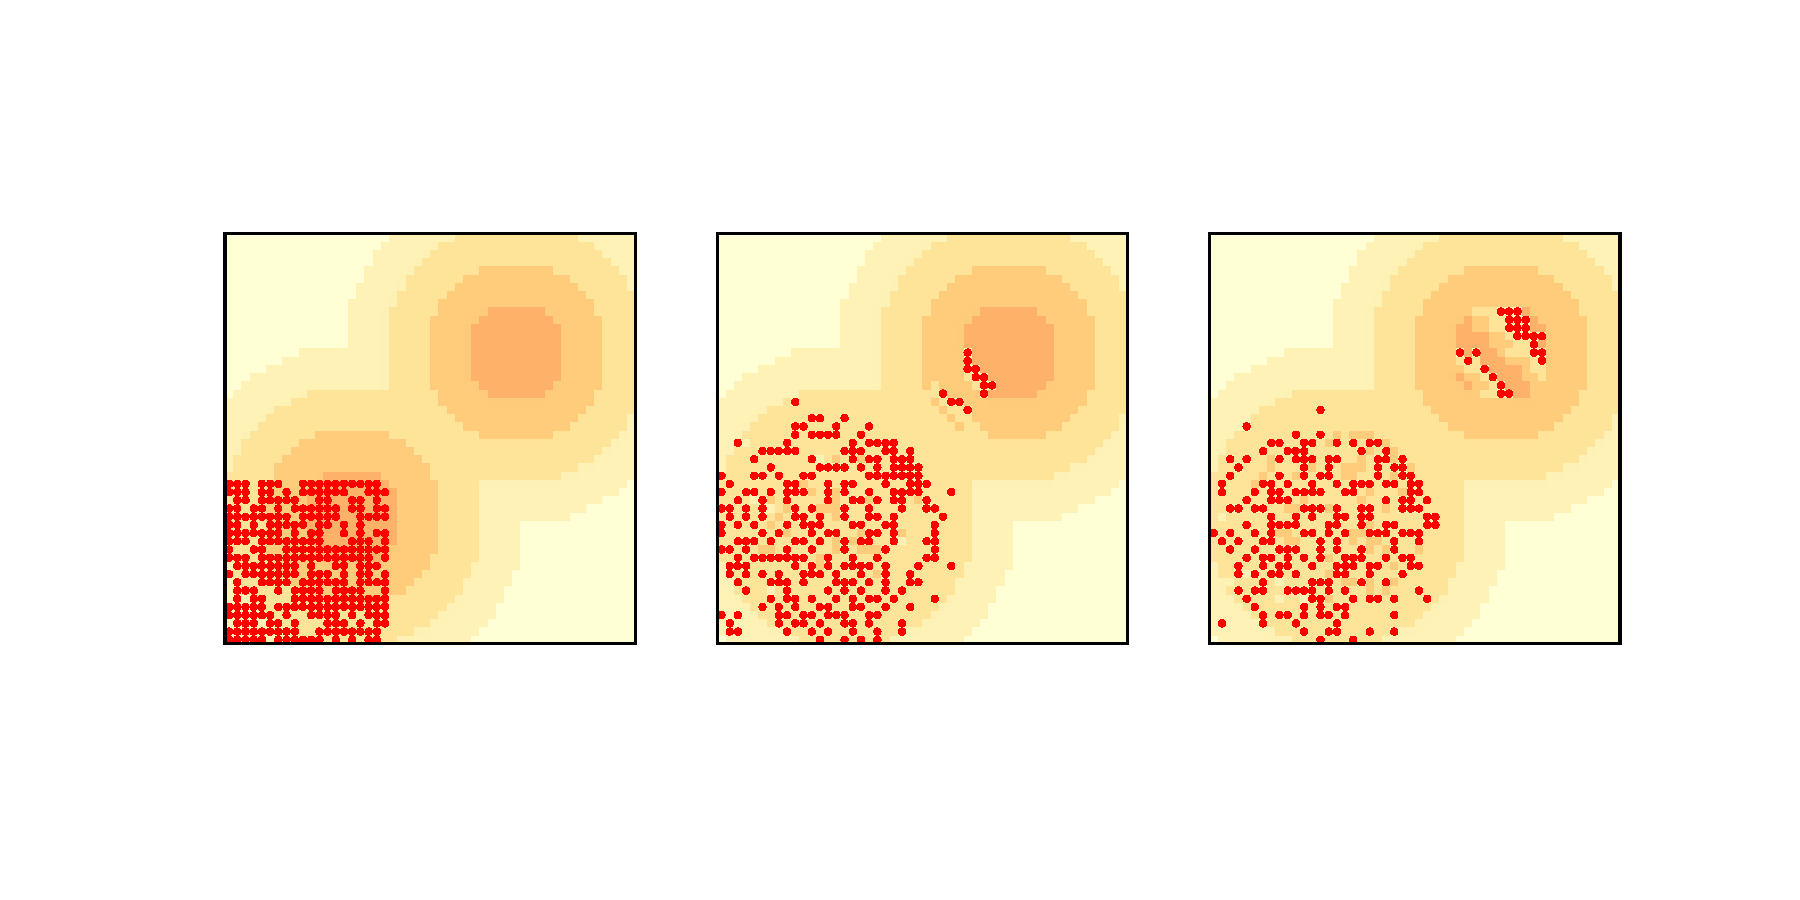
\includegraphics[height=3in]{figs/chap09-5.pdf}}
\caption{Wave behavior in Sugarscape: initial configuration (left),
after 6 steps (middle) and after 12 steps (right). }
\label{chap09-5}
\end{figure}

Although the purpose of Sugarscape is not primarily to explore the
movement of agents in space, Epstein and Axtell observed some
interesting patterns when agents migrate.

If we start with all agents in the lower-left corner, they quickly move
toward the closest ``peak'' of high-capacity cells.  But if there
are more agents than a single peak can support, they quickly exhaust
the sugar and agents are forced to move into lower-capacity areas.

The ones with the longest vision range cross the valley between the
peaks first and propagate toward the northeast in a pattern that
resembles a wave front.  Because they leave a stripe of empty cells
behind them, other agents don't follow until the sugar grows back.

The result is a series of discrete waves of migration, where each wave
resembles a coherent object, like the spaceships we saw in the Rule
110 CA and Game of Life (see Section~\ref{spaceships} and
Section~\ref{lifepatterns}).

Figure~\ref{chap09-5} shows the initial condition (left) and the
state of the model after 6 steps (middle) and 12 steps (right).
You can see the first two waves reaching and moving through the
second peak, leaving a stripe of empty cells behind.  You can also
see an animated version of this model, where the wave patterns are
more clearly visible.

Although these waves are made up of agents, we can think of them
as entities of their own, in the same way we think of gliders in
Game of Life.

An interesting property of these waves is that they
move diagonally, which might be surprising, because the agents
themselves only move north or east, never northeast.  Outcomes
like this -- groups or ``aggregates'' with properties and behaviors
that the agents don't have -- are common in agent-based models.
We will see more examples in the next chapter.


\section{Emergence}

The examples in this chapter demonstrate one of the most important
ideas in complexity science: emergence.  An {\bf emergent property} is
a characteristic of a system that results from the interaction of its
components, not from their properties.

\index{emergence}
\index{emergent property}

To clarify what emergence is, it helps to consider what it isn't.  For
example, a brick wall is hard because bricks and mortar are hard, so
that's not an emergent property.  As another example, some rigid
structures are built from flexible components, so that seems like a
kind of emergence.  But it is at best a weak kind, because structural
properties follow from well understood laws of mechanics.

\index{brick wall}

In contrast, the segregation we see in Schelling's model is an emergent
property because it is not caused by racist agents.  Even when the
agents are only mildly xenophobic, the outcome of the system is
substantially different from the intention of the agent's decisions.

The distribution of wealth in Sugarscape might be an emergent
property, but it is a weak example because we could
reasonably predict it based on the distributions of vision, metabolism,
and lifespan.  The wave behavior we saw in the last example might
be a stronger example, since the wave displays a capability -- diagonal
movement -- that the agents clearly do not have.

Emergent properties are surprising: it is hard to predict the behavior
of the system even if we know all the rules.  That difficulty is not
an accident; in fact, it may be the defining characteristic of emergence.

As Wolfram discusses in {\em A New Kind of Science}, conventional science
is based on the axiom that if you know the rules that govern a system,
you can predict its behavior.  What we call ``laws'' are often
computational shortcuts that allow us to predict the outcome of a
system without building or observing it.

\index{New Kind of Science@{\it A New Kind of Science}}
\index{Wolfram, Stephen}
\index{natural law}

But many cellular automatons are {\bf computationally irreducible},
which means that there are no shortcuts.  The only way to get the
outcome is to implement the system.

\index{computationally irreducible}
\index{shortcut}

The same may be true of complex systems in general.  For physical
systems with more than a few components, there is usually no model
that yields an analytic solution.  Numerical methods provide a kind of
computational shortcut, but there is still a qualitative difference.

Analytic solutions often provide a constant-time algorithm for
prediction; that is, the run time of the computation does not depend
on $t$, the time scale of prediction.  But numerical methods,
simulation, analog computation, and similar methods take time
proportional to $t$.  And for many systems, there is a bound on $t$
beyond which we can't compute reliable predictions at all.

These observations suggest that emergent properties are fundamentally
unpredictable, and that for complex systems we should not expect to
find natural laws in the form of computational shortcuts.

To some people, ``emergence'' is another name for ignorance; by this
reckoning, a property is emergent if we don't have a reductionist
explanation for it, but if we come to understand it better in the
future, it would no longer be emergent.

The status of emergent properties is a topic of debate, so it is
appropriate to be skeptical.  When we see an apparently emergent
property, we should not assume that there can never be a reductionist
explanation.  But neither should we assume that there has to be one.

The examples in this book and the principle of computational
equivalence give good reasons to believe that at least some emergent
properties can never be ``explained'' by a classical reductionist
model.

You can read more about emergence at
\url{http://en.wikipedia.org/wiki/Emergence}.


\section{Exercises}

\begin{exercise}

The code for this chapter is in the Jupyter notebook {\tt chap09.ipynb}
in the repository for this book.  Open this notebook, read the code,
and run the cells.  You can use this notebook to work on the
exercises in this chapter.  My solutions are in {\tt chap09soln.ipynb}.

\end{exercise}

\begin{exercise}

Bill Bishop, author of {\em The Big Sort}, argues that
American society is increasingly segregated by political
opinion, as people choose to live among like-minded neighbors.

\index{Big Sort@{\em The Big Sort}}
\index{Bishop, Bill}

The mechanism Bishop hypothesizes is not that people, like the agents
in Schelling's model, are more likely to move if they are
isolated, but that when they move for any reason, they are
likely to choose a neighborhood with people like themselves.

Modify your implementation of Schelling's model to simulate
this kind of behavior and see if it yields similar degrees of
segregation.

There are several ways you can model Bishop's hypothesis.  In my
implementation, a random selection of agents moves during each step.
Each agent considers \py{k} randomly-chosen empty locations and
chooses the one with the highest fraction of similar neighbors.
How does the degree of segregation depend on \py{k}?

\end{exercise}


\begin{exercise}

In the first version of SugarScape, we never add agents, so once the
population falls, it never recovers.  In the second version, we only
replace agents when they die, so the population is constant.  Now
let's see what happens if we add some ``population pressure''.

Write a version of SugarScape that adds a new agent at the end of
every step.  Add code to compute the average vision and the average
metabolism of the agents at the end of each step.  Run the model for a
few hundred steps and plot the population over time, as well as the
average vision and average metabolism.

You should be able to implement this model by inheriting from
\py{SugarScape} and overriding \py{__init__} and \py{step}.

\end{exercise}


\begin{exercise}

In the philosophy of mind, {\em Strong AI} is the theory that an
appropriately-programmed computer could have a mind in the same sense
that humans have minds.

John Searle presented a thought experiment called ``The Chinese Room'',
intended to show that {\em Strong AI} is false.  You can read about
it at \url{http://en.wikipedia.org/wiki/Chinese_room}.

What is the {\bf system reply} to the Chinese Room argument?
How does what you have learned about emergence influence
your reaction to the system response?

\end{exercise}



\chapter{Herds, Flocks, and Traffic Jams}

NOTE: THIS CHAPTER IS NOT DONE!

The code for this chapter is in \py{chap10.ipynb}, which is a
Jupyter notebook in the repository for this book.  For more information
about working with this code, see Section~\ref{code}.


\section{Traffic jams}

What causes traffic jams?  In some cases there is an obvious cause,
like an accident, a speed trap, or something else that disturbs
the flow of traffic.  But other times traffic jams appear for no
apparent reason.
\index{traffic jam}

Agent-based models can help explain spontaneous traffic jams.
As an example, I implemented a simple highway simulation, based on
a model in Resnick, {\em Turtles, Termites and Traffic Jams}.

\index{Turtles, Termites and Traffic Jams@{\em Turtles, Termites and Traffic Jams}}
\index{Resnick, Mitchell}

Here's the class that represents the ``highway'':

\begin{code}
class Highway:

    def __init__(self, n=10, length=1000, eps=0):
        self.length = length
        self.eps = eps

        # create the drivers
        locs = np.linspace(0, length, n, endpoint=False)
        self.drivers = [Driver(loc) for loc in locs]

        # and link them up
        for i in range(n):
            j = (i+1) % n
            self.drivers[i].next = self.drivers[j]
\end{code}

\py{n} is the number of cars.

\py{length} is the length of the
highway, which is 1000 by default (in arbitrary units).

\py{eps} is the amount of
random noise we'll add to the system.

\py{locs} contains the locations of the drivers; initially
they are equally spaced along the highway.

Finally, we link the drivers so that each driver contains a reference
to the next driver in front.  The highway is circular, so the
last driver contains a reference to the first.

The \py{step} method is simple; it just moves each of the drivers:

\begin{code}
    def step(self):
        for driver in self.drivers:
            self.move(driver)
\end{code}

And here's the \py{move} method:

\begin{code}
    def move(self, driver):
        d = self.distance(driver)

        # let the driver choose acceleration
        acc = driver.choose_acceleration(d)
        acc = min(acc, self.max_acc)
        acc = max(acc, self.min_acc)
        speed = driver.speed + acc

        # add random noise to speed
        speed *= np.random.uniform(1-self.eps, 1+self.eps)

        # keep it nonnegative and under the speed limit
        speed = max(speed, 0)
        speed = min(speed, self.speed_limit)

        # if current speed would collide, stop
        if speed > d:
            speed = 0

        # update speed and loc
        driver.speed = speed
        driver.loc += speed
\end{code}

\py{d} is the distance between \py{driver} and the next driver ahead.
This distance is passed to \py{choose_acceleration}, which
specifies the behavior of the driver.  This is the only decision the
driver gets to make; everything else is determined by the ``physics''
of the simulation.

\begin{itemize}

\item \py{acc} is acceleration, which limited by \py{min_acc} and
  \py{max_acc}.  In my implementation, cars can accelerate with
  \py{max_acc=1} and brake with \py{min_acc=-10}.

\item \py{speed} is the old speed plus the requested acceleration, but
then we make some adjustments.  First, we add random noise to
\py{speed}, because the world is not perfect.  \py{eps} determines the magnitude
of the noise, which is a percentage applied to \py{speed}; for example, if
\py{eps} is 0.02, \py{speed} is muliplied by a random number between 98\%
and 102\%.

\item Then speed is bounded between 0 and \py{speed_limit}, which is
40 in my implementation, so cars are not allowed to go backward or speed.

\item If the requested speed would cause a collision with the next car,
\py{speed} is set to 0.

\item Finally, we update the \py{speed} and \py{loc}
attributes of \py{driver}.

\end{itemize}

Here's the definition for the \py{Driver} class:

\begin{code}
class Driver:

    def __init__(self, loc, speed=0):
        self.loc = loc
        self.speed = speed

    def choose_acceleration(self, d):
        return 1
\end{code}

The attributes \py{loc} and \py{speed} are the location and speed of the
driver.

This implementation of \py{choose_acceleration} is very simple:
it always accelerates at the maximum rate.

Since the cars start out equally spaced, we expect them all to
accelerate until they reach the speed limit, or until their speed
exceeds the space between them.  At that point, at least one
``collision'' will occur, causing some cars to stop.

\begin{figure}
\centerline{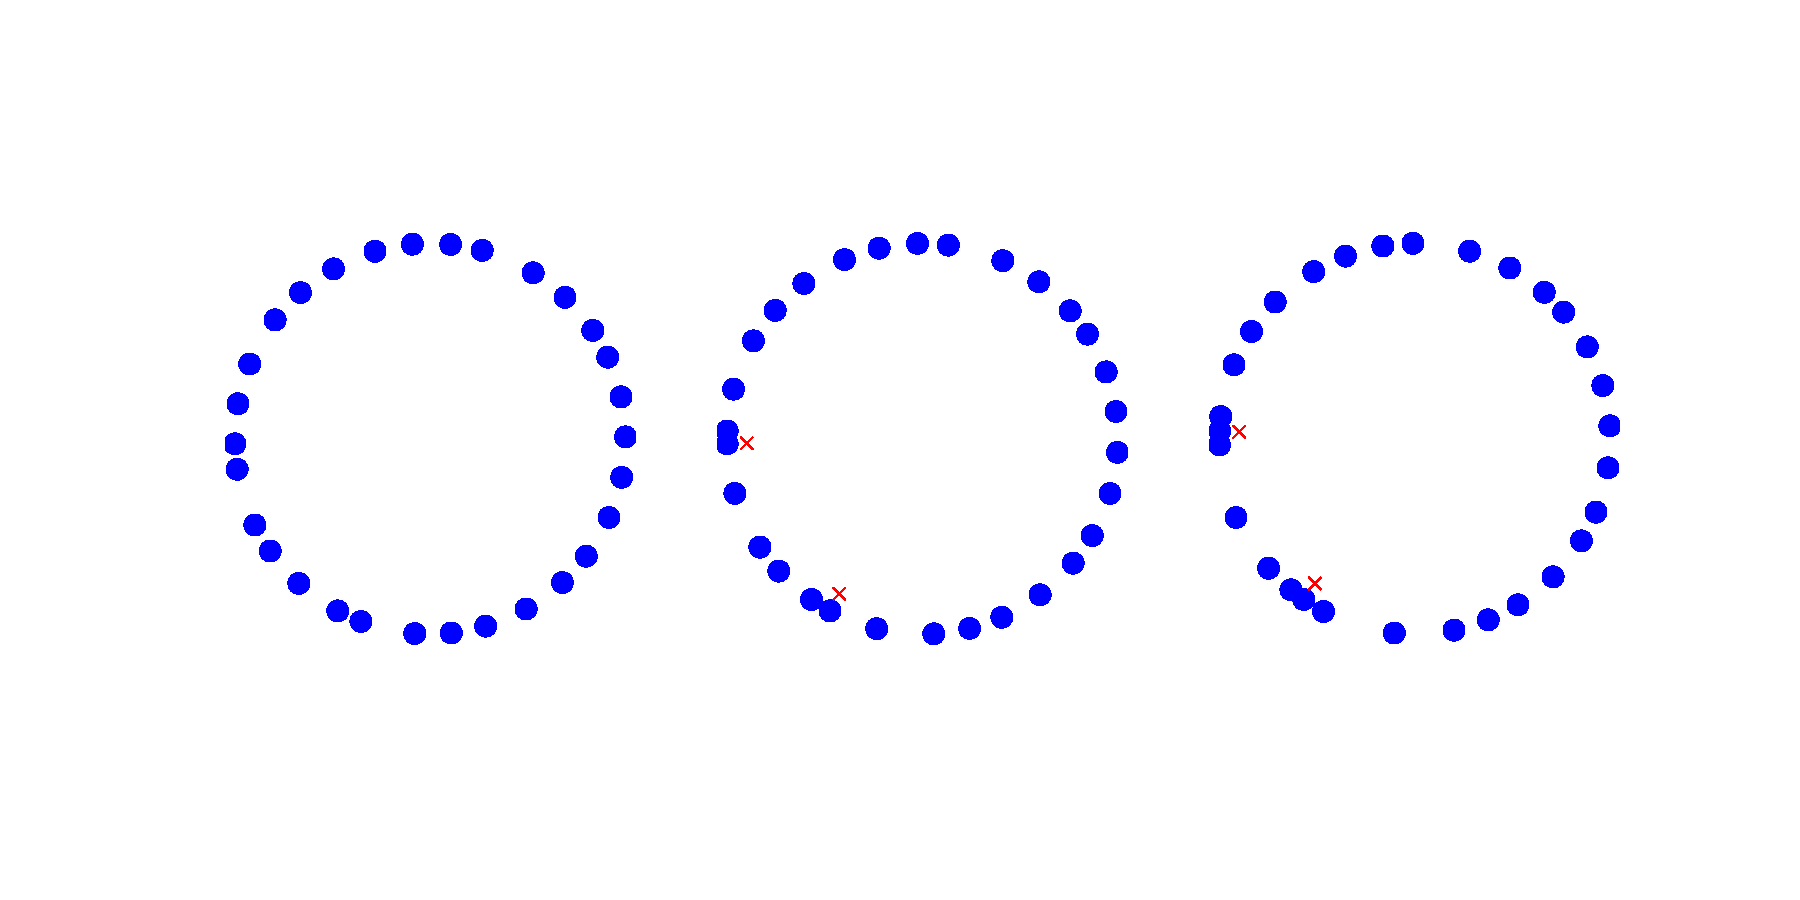
\includegraphics[height=3in]{figs/chap10-1.pdf}}
\caption{}
\label{chap10-1}
\end{figure}

Figure~\ref{chap10-1} shows a few steps in this process, starting with
30 cars and \py{eps=0.02}.  On the left is the configuration after
16 time steps, with the cars arranged in a circle.
Because of random noise, some cars are going faster
than others, and the spacing has become uneven.

During the next time step (center) two cars collide, indicated
by the \py{x} marks.

During the next time step (right) two cars collide with the stopped
cars, and we can see the initial formation of a traffic jam.  Once
a jam forms, it tends to persist, with additional cars approaching from
behind and colliding, and with the cars in the front accelerating
away.

Under some conditions, the jam itself propagates backwards, as you
can see if you watch the animations in the notebook for this chapter.



\section{Random Noise}

\begin{figure}
\centerline{\includegraphics[height=3in]{figs/chap10-2.pdf}}
\caption{}
\label{chap10-2}
\end{figure}

As the number of cars increases, traffic jams become more severe.
Figure~\ref{chap10-2} shows the average speed cars are able to
achieve, as a function of the number of cars.

The top line shows results with \py{eps=0}; that is, with no random
variation in speed.  With 25 or fewer cars, the spacing between
cars is greater than 40, which allows cars to reach and maintain
the maximum speed, which is 40.  With more than 25 cars, traffic
jams form and the average speed drops quickly.

This effect is a direct result of the physics of the simulation,
so it should not be surprising.  If the length of the road is
1000, the spacing between \py{n} cars is \py{1000/n}.  And since cars
can't move faster than the space in front of them, the highest
average speed we expect is \py{1000/n} or 40, whichever is less.

But that's the best case scenario.  With just a small amount of
randomness, things get much worse.

Figure~\ref{chap10-2} also shows results with \py{eps=0.001} and
\py{eps=0.01}, which correspond to errors in speed of 0.1\% and 1\%.

With even a small amount of noise, the capacity of the highway
drops from 25 to 20 (by ``capacity'' I mean the maximum number
of cars that can reach and sustain the speed limit).  And
with 1\% errors, the capacity drops to 10.  Ugh.

As one of the exercises at the end of this chapter, you'll have a
chance to design a better driver; that is, you will experiment with
different strategies in \py{choose_acceleration} and see if you can
find driver behaviors that improve average speed.


\section{Boids}

In 1987 Craig Reynolds published ``Flocks, herds and
schools: A distributed behavioral model'', which describes an
agent-based model of herd behavior.  You can download his
paper from \url{http://www.red3d.com/cwr/papers/1987/boids.html}.

\index{Reynolds, Craig}

Agents in this models are called ``boids'', which is both a
contraction of ``bird-oid'' and an accented pronunciation of ``bird''
(although boids are also used to model fish and herding land animals).

\index{boid}

Each agent simulates three behaviors:

\begin{description}

\item[Collision avoidance:] Avoid obstacles, including other birds.

\item[Flock centering:] Move toward the center of the flock.

\item[Velocity matching:] Align velocity (speed and direction) with neighboring birds.

\end{description}

Boids make decisions based on local information only; each boid
only sees (or pays attention to) other boids in its field of
vision and range.

\index{local information}

In the repository for this book, you will find {\tt Boids7.py}, which contains my implementation of boids, based in part
on the description in Flake, {\em The Computational
Beauty of Nature}.

The program defines two classes: \py{Boid}, which implements the boid
algorithm, and \py{World}, which contains a list of Boids and a
``carrot'' the Boids are attracted to.
\index{carrot}

The boid algorithm uses \py{get_neighbors} to find other
boids in the field of view:

\begin{code}
    def get_neighbors(self, others, radius, angle):
        boids = []
        for other in others:
            if other is self:
               continue

            offset = other.pos - self.pos

            # if not in range, skip it
            if offset.mag > radius:
                continue

            # if not within viewing angle, skip it
            if self.vel.diff_angle(offset) > angle:
                continue

            # otherwise add it to the list
            boids.append(other)

        return boids
\end{code}

\py{get_neighbors} uses vector subtraction to compute the
vector from \py{self} to \py{other}.  The magnitude of
this vector is the distance to the other boid.  \py{diff_angle}
computes the angle between the velocity of \py{self}, which
is also the line of sight, and the other boid.

\py{center} finds the center of mass of the boids in the
field of view and returns a vector pointing toward it:

\begin{code}
    def center(self, others):
        close = self.get_neighbors(others, r_center, a_center)
        t = [other.pos for other in close]
        if t:
            center = sum(t)/len(t)
            toward = vector(center - self.pos)
            return limit_vector(toward)
        else:
            return null_vector
\end{code}

Similarly, \py{avoid} finds the center of mass of any obstacles
in range and returns a vector pointing away from it,
\py{copy} returns the difference between the current heading
and the average heading of the neighbors, and \py{love}
computes the heading toward the carrot.

\py{set_goal} computes the weighed sum of these goals and
sets the overall goal:

\begin{code}
    def set_goal(self, boids, carrot):
        self.goal = (w_avoid * self.avoid(boids, carrot) +
                     w_center * self.center(boids) +
                     w_copy * self.copy(boids) +
                     w_love * self.love(carrot))
\end{code}

Finally, \py{move} updates the velocity, position and
attitude of the boid:

\begin{code}
    def move(self, mu=0.1):
        self.vel = (1-mu) * self.vel + mu * self.goal
        self.vel.mag = 1

        self.pos += dt * self.vel
        self.axis = b_length * self.vel.norm()
\end{code}

The new velocity is the weighted sum of the old velocity
and the goal.  The parameter \py{mu} determines how quickly
the birds can change speed and direction.  The time step, \py{dt},
determines how far the boids move.
\index{weighted sum}

Many parameters influence flock behavior, including the range, angle
and weight for each behavior, and the maneuverability, \py{mu}.
\index{flock behavior}

These parameters determine the ability of the boids to form and
maintain a flock and the patterns of motion and organization in the
flock.  For some settings, the boids resemble a flock of birds; other
settings resemble a school of fish or a cloud flying insects.


\section{Emergence and free will}
\label{freewill}


%TODO: expand this based on class discussion


Many complex systems have properties, as a whole, that their
components do not:

\begin{itemize}

\item The Rule 30 cellular automaton is deterministic, and the rules
  that govern its evolution are completely known.  Nevertheless, it
  generates a sequence that is statistically indistiguishable from
  random.

\item The agents in Schelling's model are not racist, but the outcome
  of their interactions is as if they were.

\item Agents in Sugarscape form waves that move diagonally even
though the agents cannot.

\item Traffic jams move backward even though the cars in them are
  moving forward.

\item The behavior of flocks and herds emerges from local interactions
  between their members.

\end{itemize}

These examples suggest an approach to several old and challenging
questions, including the problems of consciousness and free will.

Free will is the ability to make choices, but if our bodies and brains
are governed by deterministic physical laws, our choices would be
determined.  Arguments about free will are innumerable; I will
only mention two:

\begin{itemize}

\item William James proposed a two-stage model in which
  possible actions are generated by a random process and then selected
  by a deterministic process.  In that case our actions are
  fundamentally unpredictable because the process that generates them
  includes a random element.

\item David Hume suggested that our perception of making choices
  is an illusion; in that case, our actions are deterministic because
  the system that produces them is deterministic.

\end{itemize}

These arguments reconcile the conflict in opposite ways, but they
agree that there is a conflict: the system cannot have free will if
the parts are deterministic.

The complex systems in this book suggest the alternative
that free will, at the level of options and decisions, is compatible
with determinism at the level of neurons (or some lower level).  In
the same way that a traffic jam moves backward while the cars move
forward, a person can have free will even though neurons don't.


\section{Exercises}

\begin{exercise}

In the traffic jam simulation, define a class, \py{BetterDriver},
that inherits from \py{Driver} and overrides \py{choose_acceleration}.
See if you can define driving rules that do better than the basic
implementation in \py{Driver}.  You might try to achieve higher
average speed, or a lower number of collisions.

% TODO: Add a crash counter.  Maybe pass the Highway object to
% choose_acceleration

\end{exercise}



\begin{exercise}

Note: To do this exercise, you will have to install VPython, a library for 3D displays and animation.  If you use Anaconda (as I recommend in Section~\ref{code}), you can run:

\begin{code}
conda install -c vpython vpython
\end{code}

Then run \py{Boids7.py}, which is in the repository for this book.  Read the code to see how the parameters defined at the beginning of the program control boid behaviors.  Experiment with
different parameters.  What happens if you ``turn off'' one
of the behaviors by setting the weight to 0?
\index{parameter}

To generate more bird-like behavior, Flake suggests adding a fourth
behavior to maintain a clear line of sight; in other words, if there
is another bird directly ahead, the boid should move away
laterally.  What effect do you expect this rule to have on the
behavior of the flock?  Implement it and see.

\end{exercise}


\begin{exercise}

Read more about free will at
\url{http://en.wikipedia.org/wiki/Free_will}.  The view that free will
is compatible with determinism is called {\bf compatibilism}.  One of
the strongest challenges to compatibilism is the ``consequence
argument''.  What is the consequence argument?  What response can you
give to the consequence argument based on what you have read in this
book?

\end{exercise}





\chapter{Evolution}

The most important idea in biology, and possibly all of science, is the {\bf theory of evolution by natural selection}, which claims that new species are created, and existing species change over time, due to natural selection.  Natural selection is a process in which heritable differences between individuals cause differences in survival or reproduction (or both).

Among people who know something about biology, the theory of evolution is widely regarded as a fact, which is to say that it close enough to the truth that if it is corrected in the future, the amendments will leave the central ideas substantially intact.

Nevertheless, many people do not believe in evolution.  In a survey run by the Pew Research Center, survey respondents were asked which of the following claims is closer to their view:

\begin{enumerate}

\item Humans and other living things have evolved over time.

\item Humans and other living things have existed in their present form since the beginning of time.

\end{enumerate}

About 34\% of Americans chose the second (see \url{http://www.thearda.com/Archive/Files/Codebooks/RELLAND14_CB.asp}).

Even among the ones who believe that living things have evolved, barely more than half believe that the cause of evolution is natural selection.  In other words, only about 33\% of Americans believe that the theory of evolution is true.

How is this possible?  In my opinion, contributing factors include:

\begin{itemize}

\item Some people think that there is a conflict between evolution and their religious beliefs and, feeling like they have to reject one, they reject evolution.

\item Others have been actively misinformed, often by members of the first group, so that much of what they know about evolution is false.

\item And many people simply don't know anything about evolution.

\end{itemize}

There's probably not much I can do about the first group, but I think I can help the others.  Empirically, the theory of evolution is hard for people to understand.  At the same time, it is profoundly simple: for many people, once they understand it, it seems both obvious and irrefutable.

To help people make this transition from confusion to clarity, the most powerful tool I have found is computation.  Ideas that are hard to understand in theory can be easy to understand when we see them happening in simulation.
That is the goal of this chapter.

The code for this chapter is in \py{chap11.ipynb}, which is a
Jupyter notebook in the repository for this book.  For more information
about working with this code, see Section~\ref{code}.


\section{Simulating evolution}

I will start with a simple model that demonstrates a basic form of evolution.  According to the theory, the following features are sufficient to produce evolution:

\begin{itemize}

\item Replicators:  We need a population of agents that can reproduce in some way.  We'll start with replicators that make perfect copies of themselves.  Later we'll add imperfect copying, that is, mutation.

\item Variation:  We also need some variability in the population, that is, differences between individuals.

\item Differential survival or reproduction:  The differences between individuals have to affect their ability to survive or reproduce.

\end{itemize}

To simulate these features, we'll define a population of {\bf agents} that represent individual organisms.  Each agent has genetic information, called its {\bf genotype}, which is the information that gets copied when the agent replicates.  In our model\footnote{This model is a variant of the NK model developed primarily by Stuart Kauffman (see \url{https://en.wikipedia.org/wiki/NK_model})}, a genotype is represented by a sequence of \py{N} binary digits (zeros and ones), where \py{N} is a parameter we can choose.

To generate a population with variation, we choose initial genotypes at random; later we will explore mechanisms that generate or increase variation.

Finally, to generate differential survival and reproduction, we define a function that maps from each genotype to a {\bf fitness}, where fitness is a quantity related to the ability of an agent to survive or reproduce.

\section{Fitness landscape}

The function that maps from genotype to fitness is called a {\bf fitness landscape}.  In the landscape metaphor, each genotype corresponds to a location in an \py{N}-dimensional space, and fitness corresponds to the ``height" of the landscape at that location.  For visualizations that might clarify this metaphor, see \url{https://en.wikipedia.org/wiki/Fitness_landscape}.

In biological terms, the fitness landscape represents information about how the genotype of an organism is related to its physical form and capabilities, called its {\bf phenotype}, and how the phenotype interacts with its {\bf environment}.

In the real world, fitness landscapes are complicated, but we don't need to build a realistic model.  To induce evolution, we need {\em some} relationship between genotype and fitness, but it turns out that it can be {\em any} relationship.  To demonstrate this point, we'll generate the fitness function at random.

Here is the definition for a class that represents a fitness landscape:

\begin{code}
class FitnessLandscape:
    def __init__(self, N):
        self.N = N
        self.one_values = np.random.random(N)
        self.zero_values = np.random.random(N)

    def fitness(self, loc):
        fs = np.where(loc, self.one_values,
                           self.zero_values)
        return fs.mean()
\end{code}

The genotype of an agent, which corresponds to its location in the fitness landscape, is represented by a NumPy array of zeros and ones, called \py{loc}.
The fitness of a given genotype is the mean of \py{N} {\bf fitness contributions}, one for each element of \py{loc}.

To compute the fitness of a genotype, \py{FitnessLandscape} uses two arrays:
\py{one_values}, which contains the fitness contributions of having a \py{1} in each element of \py{loc}, and \py{zero_values}, which contains the fitness contributions of having a \py{0}.

The \py{fitness} method uses \py{np.where} to select a value from \py{one_values} where \py{loc} has a \py{1}, and a value from \py{zero_values} where \py{loc} has a \py{0}.

As an example, suppose \py{N=3} and

\begin{code}
one_values =  [0.1, 0.2, 0.3]
zero_values = [0.4, 0.7, 0.9]
\end{code}

In that case, the fitness of \py{loc = [0, 1, 0]} would be the mean of \py{[0.4, 0.2, 0.9]}, which is \py{0.5}.


\section{Agents}

Next we need agents.  Here's the class definition:

\begin{code}
class Agent:

    def __init__(self, loc, fit_land):
        self.loc = loc
        self.fit_land = fit_land
        self.fitness = fit_land.fitness(self.loc)

    def copy(self):
        return Agent(self.loc, self.fit_land)
\end{code}

The attributes of an \py{Agent} are:

\begin{itemize}

\item \py{loc}: The location of the \py{Agent} in the fitness landscape.

\item \py{fit_land}: A reference to a \py{FitnessLandscape} object.

\item \py{fitness}: The fitness of this \py{Agent} in the \py{FitnessLandscape}, represented as a number between 0 and 1.

\end{itemize}

This definition of \py{Agent} provides a simple \py{copy} method that copies the genotype exactly; later, we will see a version that copies with mutation, but mutation is not necessary for evolution.


\section{Simulation}
\label{evosim}

Now that we have agents and a fitness landscape, I'll define a class called \py{Simulation} that simulates the creation, reproduction, and death of the agents.  To avoid getting bogged down, I'll present a simplified version of the code here; you can see the details in the notebook for this chapter.

Here's the definition of \py{Simulation}:

\begin{code}
class Simulation:

    def __init__(self, fit_land, agents):
        self.fit_land = fit_land
        self.agents = agents
\end{code}

The attributes of a \py{Simulation} are:

\begin{itemize}

\item \py{fit_land}: A reference to a \py{FitnessLandscape} object.

\item \py{agents}: An array of \py{Agent} objects.

\end{itemize}

The most important function in \py{Simulation} is \py{step}, which simulates one time step:

\begin{code}
# class Simulation:

    def step(self):
        n = len(self.agents)
        fits = self.get_fitnesses()

        # see who dies
        index_dead = self.choose_dead(fits)
        num_dead = len(index_dead)

        # replace the dead with copies of the living
        replacements = self.choose_replacements(num_dead, fits)
        self.agents[index_dead] = replacements
\end{code}

\py{step} uses three other methods:

\begin{itemize}

\item \py{get_fitnesses} returns an array containing the fitness of each agent in the order they appear in the agent array.

\item \py{choose_dead} decides which agents die during this timestep, and returns an array that contains the indices of the dead agents.

\item \py{choose_replacements} decides which agents reproduce during this timestep, invokes \py{copy} on each one, and returns an array of new \py{Agent} objects.

\end{itemize}

In this version of the simulation, the number of new agents during each timestep equals the number of dead agents, so the number of live agents is constant.


\section{No differentiation}

Before we run the simulation, we have to specify the behavior of \py{choose_dead} and \py{choose_replacements}.  We'll start with simple versions of these functions that don't depend on fitness:

\begin{code}
# class Simulation

     def choose_dead(self, fits):
        n = len(self.agents)
        is_dead = np.random.random(n) < 0.1
        index_dead = np.nonzero(is_dead)[0]
        return index_dead

    def choose_replacements(self, n, fits):
        agents = np.random.choice(self.agents, size=n, replace=True)
        replacements = [agent.copy() for agent in agents]
        return replacements
\end{code}

In \py{choose_dead}, \py{n} is the number of agents; \py{is_dead} is a boolean array that contains \py{True} for the agents who die during this time step.  In this version, every agents has the same chance of dying: 10\%.

\py{choose_dead} uses \py{np.nonzero} to find the indices of the non-zero elements of \py{is_dead} (\py{True} is considered non-zero).

In \py{choose_replacements}, \py{n} is the number of agents who reproduce during this time step.  It uses \py{np.random.choice} to choose \py{n} agents, with replacement.  Then it invokes \py{copy} on each one and returns a list of new \py{Agent} objects.

These methods don't depend on fitness, so this simulation does not have differential survival or reproduction.  As a result, we should not expect to see evolution.  But how can we tell?

\section{Evidence of evolution}
\label{instrument}

The most inclusive definition of evolution is a change in the distribution of genotypes in a population.  So evolution is an aggregate effect: in other words, individuals don't evolve; populations do.

In this simulation, genotypes are locations in a high-dimensional space, so it is hard to visualize changes in their distribution.  However, if the genotypes change, we expect their fitness to change as well.  So we will use changes in the distribution of fitness as evidence of evolution.  In particular, we'll look at the mean and standard deviation of fitness across the population.

Before we run the simulation, we have to add an \py{Instrument}, which is an object that gets updated after each time step, computes some statistic of interest, and stores the result in a sequence we can plot later.

Here is the parent class for all instruments:

\begin{code}
class Instrument:
    def __init__(self):
        self.metrics = []
\end{code}

And here's the definition for \py{MeanFitness}, an instrument that computes the mean fitness of the population at each time step:

\begin{code}
class MeanFitness(Instrument):
    def update(self, sim):
        mean = np.nanmean(sim.get_fitnesses())
        self.metrics.append(mean)
\end{code}

Now we're ready to run the simulation.  To minimize the effect of random changes in the starting population, we'll start every simulation with the same set of agents.  And to make sure we explore the entire fitness landscape, we'll start with one agent at every location.  Here's the code that creates the \py{Simulation}:

\begin{code}
N = 8
fit_land = FitnessLandscape(N)
agents = make_all_agents(fit_land, Agent)
sim = Simulation(fit_land, agents)
\end{code}

\py{make_all_agents} creates one \py{Agent} for every location; the implementation is in the notebook for this chapter.

Now we can create and add a \py{MeanFitness} instrument, run the simulation, and plot the results:

\begin{code}
instrument = MeanFitness()
sim.add_instrument(instrument)
sim.run()
sim.plot(0)
\end{code}

The \py{Simulation} keeps a list of \py{Instrument} objects.  After each timestep it invokes \py{update} on each \py{Instrument} in the list.

After the simulation runs, we plot the results using \py{Simulation.plot}, which takes an index as a parameter, uses the index to select an \py{Instrument} from the list, and plots the results.  In this example, there is only one \py{Instrument}, so the index is 0.

\begin{figure}
\centerline{\includegraphics[height=3in]{figs/chap11-1.pdf}}
\caption{Mean fitness over time for 10 simulations with no differential survival or reproduction.}
\label{chap11-1}
\end{figure}

Figure~\ref{chap11-1} shows the results of running this simulation with the \py{MeanFitness} instrument 10 times.  The mean fitness of the population drifts up or down, due to chance.  Since the distribution of fitness changes over time, we infer that the distribution of phenotypes is also changing.  By the most inclusive definition, this {\bf random walk} is a kind of evolution.  But it is not a particularly interesting kind.

In particular, this kind of evolution does not explain how biological species change over time, or how new species appear.  The theory of evolution is powerful because it explains phenomena we see in the natural world that seem inexplicable:

\begin{itemize}

\item Adaptation: Species interact with their environments in ways that seem too complex, too intricate, and too clever to happen by chance.  Many features of natural systems seem as if they were designed.

\item Increasing diversity: Over time the number of species on earth has generally increased (despite several periods of mass extinction).

\item Increasing complexity: The history of life on earth starts with relatively simple life forms, with more complex organisms appearing later in the geological record.

\end{itemize}

These are the phenomena we want to explain.  So far, our model doesn't do the job.


\section{Differential survival}
\label{diffsurv}

So let's add one more ingredient, differential survival.  Here's the definition for a class that extends \py{Simulation} and overrides \py{choose_dead}:

\begin{code}
class SimWithDiffSurvival(Simulation):

    def choose_dead(self, fits):
        n = len(self.agents)
        is_dead = np.random.random(n) > fits
        index_dead = np.nonzero(is_dead)[0]
        return index_dead
\end{code}

Now the probability of survival depends on fitness; in fact, in this version, the probability that an agent survives each time step {\em is} its fitness.

Since agents with low fitness are more likely to die, agents with high fitness are more likely to survive long enough to reproduce.  So we expect the number of low-fitness agents to decrease, and the number of high-fitness agents to increase.  If we plot the mean fitness over time, we expect it to increase.

\begin{figure}
\centerline{\includegraphics[height=3in]{figs/chap11-2.pdf}}
\caption{Mean fitness over time for 10 simulations with differential survival.}
\label{chap11-2}
\end{figure}

Figure~\ref{chap11-2} shows the results of 10 simulations with differential survival.  Mean fitness increases quickly at first, but then levels off.

You can probably figure out why it levels off: if there is only one agent at a particular location and it dies, it leaves that location unoccupied.  And without mutation, there is no way for it to be occupied again.

With \py{N=8}, this simulation starts with 256 agents occupying all possible locations.  Over time, the number of occupied locations decreases; if the simulation runs long enough, eventually all agents will occupy the same location.

So this simulation starts to explain adaptation: increasing fitness means that the species is getting better at surviving in its environment.  But with a decreasing number of locations, it does not explain increasing diversity at all.

In the notebook for this chapter, you will see the effect of differential reproduction.  As you might expect, differential reproduction also increases mean fitness.  But without mutation, we still don't see increasing diversity.

\section{Mutation}

In the simulations so far, we start with the maximum possible diversity --- one agent at every location in the landscape --- and end (eventually) with the minimum possible diversity, all agents at one location.

That's almost the opposite of what happened in the natural world, which apparently began with a single species that branched, over time, into the millions, or possibly billions, of species on Earth today (see \url{https://en.wikipedia.org/wiki/Global_biodiversity}).

With perfect copying in our model, we never see increasing diversity.  But if we add mutation, along with differential survival and reproduction, we get a step closer to understanding evolution in nature.

Here is a class definition that extends \py{Agent} and overrides \py{copy}:

\begin{code}
class Mutant(Agent):

    prob_mutate = 0.05

    def copy(self):
        if np.random.random() > self.prob_mutate:
            loc = self.loc.copy()
        else:
            direction = np.random.randint(self.fit_land.N)
            loc = self.mutate(direction)
        return Mutant(loc, self.fit_land)
\end{code}

In this model of mutation, every time we call \py{copy}, there is a 5\% chance of mutation.  In case of mutation, we choose a random direction from the current location --- that is, a random bit in the genotype --- and flip it.  Here's \py{mutate}:

\begin{code}
    def mutate(self, direction):
        new_loc = self.loc.copy()
        new_loc[direction] ^= 1
        return new_loc
\end{code}

The operator \py{^=} computes ``exclusive OR", which has the effect of flipping a bit (see \url{https://en.wikipedia.org/wiki/Exclusive_or#Bitwise_operation}).

Now that we have mutation, we don't have to start with an agent at every location.  Instead, we can start with the minimum variability: all agents at the same location.

\begin{figure}
\centerline{\includegraphics[height=3in]{figs/chap11-3.pdf}}
\caption{Mean fitness over time for 10 simulations with mutation and differential survival and reproduction.}
\label{chap11-3}
\end{figure}

Figure~\ref{chap11-3} shows the results of 10 simulations with mutation and differential survival and reproduction.  In every case, the population evolves toward the location with maximum fitness.

\begin{figure}
\centerline{\includegraphics[height=3in]{figs/chap11-4.pdf}}
\caption{Number of occupied locations over time for 10 simulations with mutation and differential survival and reproduction.}
\label{chap11-4}
\end{figure}

To measure diversity in the population, we can plot the number of occupied locations after each timestep.  Figure~\ref{chap11-4} shows the results.  We start with 100 agents, all at the same location.  As mutations occur, the number of occupied locations increases quickly.

When an agent discovers a high-fitness location, it is more likely to survive and reproduce.  Agents at lower-fitness locations eventually die out.  Over time, the population migrates through the landscape until most agents are at the location with the highest fitness.

At that point, the system reaches an equilibrium where mutation occupies new locations at the same rate that differential survival causes lower-fitness locations to be left empty.

The number of occupied locations in equilibrium depends on the mutation rate and the degree of differential survival.  In these simulations the number of unique occupied locations at any point is typically 5--15.

It is important to remember that the agents in this model don't move, just as the genotype of an organism doesn't change.  When an agent dies, it can leave a location unoccupied.  And when a mutation occurs, it can occupy a new location.

As agents disappear from some locations and appear in others, the population migrates across the landscape, like a glider in Game of Life.  But organisms don't evolve; populations do.


\section{Speciation}

The theory of evolution says that natural selection changes existing species and creates new ones.  In our model, we have seen changes, but we have not seen a new species.  It's not even clear, in the model, what a new species would look like.

Among species that reproduce sexually, two organisms are considered the same species if they can breed and produce fertile offspring.  But the agents in the model don't reproduce sexually, so this definition doesn't apply.

Among organisms that reproduce asexually, like bacteria, the definition of species is not as clear-cut.  Generally, a population is considered a species if their genotypes form a cluster, that is, if the genetic differences within the population are small compared to the differences between populations.

So before we can model new species, we need the ability to identify clusters of agents in the landscape, which means we need a definition of {\bf distance} between locations.  Since locations are represented with strings of binary digits, we'll define distance as the number of bits in the genotype that differ.  \py{FitnessLandscape} provides a \py{distance} method:

\begin{code}
# class FitnessLandscape

    def distance(self, loc1, loc2):
        return np.sum(np.logical_xor(loc1, loc2))
\end{code}

\begin{figure}
\centerline{\includegraphics[height=3in]{figs/chap11-5.pdf}}
\caption{Mean distance between agents over time.}
\label{chap11-5}
\end{figure}

The \py{logical_xor} function computes ``exclusive OR", which is \py{True} for the elements of the locations that differ, and \py{False} for the elements that are the same.

To quantify the dispersion of a population, we can compute the mean of the distances between every pair of agents.  In the notebook for this chapter, you'll see the \py{MeanDistance} instrument, which computes this metric after each time step.

Figure~\ref{chap11-5} shows mean distance between agents over time.  Because we start with identical mutants, the initial distances are 0.  As mutations occur, mean distance increases, reaching a maximum while the population migrates across the landscape.

Once the agents discover the optimal location, mean distance decreases until the population reaches an equilibrium where increasing distance due to mutation is balanced by decreasing distance as agents far from the optimal location are more likely to die.  In these simulations, the mean distance in equilibrium is near 1.5; that is, most agents are only 1--2 mutations away from optimal.

Now we are ready to look for new species.  To model a simple kind of speciation, suppose a population evolves in an unchanging environment until it reaches steady state (like some species we find in nature that seem to have changed very little over long periods of time).

Now suppose we either change the environment or transport the population to a new environment.  Some features that increased fitness in the old environment might decrease it in the new environment, and vice versa.

We can model these scenarios by running a simulation until the population reaches steady state, then changing the fitness landscape, and then resuming the simulation until the population reaches steady state again.

\begin{figure}
\centerline{\includegraphics[height=3in]{figs/chap11-6.pdf}}
\caption{Mean fitness over time.  After 500 timesteps, we change the fitness landscape.}
\label{chap11-6}
\end{figure}

Figure~\ref{chap11-6} shows results from a simulation like that.  Again, we start with 100 identical mutants at a random location, and run the simulation for 500 timesteps.  At that point, many agents are at the optimal location, which has fitness near 0.65, in this example.  And the genotypes of the agents form a cluster, with the mean distance between agents near 1.

After 500 steps, we run \py{FitnessLandscape.set_values}, which changes the mapping from genotype to fitness; then we resume the simulation.  Mean fitness drops immediately, because the optimal location and its neighbors in the old landscape are no better than random locations in the new landscape.

However, mean fitness increases quickly as the population migrates across the new landscape, eventually finding the new optimal location, which has fitness near 0.75 (which happens to be higher in this example, but needn't be).

Once the population reaches steady state, it forms a new cluster, with mean distance between agents near 1 again.

Now if we compute the distance between the agents' locations before and after the change, they differ by more than 6, on average.  The distances between clusters are much bigger than the distances between agents in each cluster, so we can interpret these clusters as distinct species.


\section{Summary}

We have seen that mutation, along with differential survival and reproduction, is sufficient to cause increasing fitness, increasing diversity, and a simple form of speciation.  This model is not meant to be realistic; evolution in natural systems is much more complicated than this.  Rather, it is meant to be a ``sufficiency theorem"; that is, a demonstration that the features of the model are sufficient to produce the behavior we are trying to explain (see \url{https://en.wikipedia.org/wiki/Necessity_and_sufficiency}).

Logically, this ``theorem" doesn't prove that evolution in nature is caused by these mechanisms alone.  But since these mechanisms do appear, in many forms, in biological systems, it is reasonable to think that they at least contribute to natural evolution.

Likewise, the model does not prove that these mechanisms always cause evolution.  But the results we see here turn out to be robust: in almost any model that includes these features --- imperfect replicators, variability, and differential reproduction --- evolution happens.

I hope this observation helps to demystify evolution.  When we look at natural systems, evolution seems complicated.  And because we primarily see the results of evolution, with only glimpses of the process, it can be hard to imagine and sometimes hard to believe.

But in simulation, we see the whole process, not just the results.  And by including the minimal set of features to produce evolution --- temporarily ignoring the vast complexity of biological life --- we can see evolution as the surprisingly simple, inevitable idea that it is.


\section{Exercises}

\begin{exercise}

The code for this chapter is in the Jupyter notebook {\tt chap11.ipynb}
in the repository for this book.  Open this notebook, read the code,
and run the cells.  You can use this notebook to work on the
exercises in this chapter.  My solutions are in {\tt chap11soln.ipynb}.

\end{exercise}


\chapter{Evolution of cooperation}

In this final chapter, we take on two questions, one from biology and one from philosophy:

\begin{itemize}

\item In biology, the ``problem of altruism" is the apparent conflict between natural selection, which suggests that animals live in a state of constant competition to survive and reproduce, and altruism, which is the tendency of many animals to help other animals, even to their apparent detriment.  See \url{https://en.wikipedia.org/wiki/Altruism_(biology)}.

\item In moral philosophy, the question of human nature asks whether humans are fundamentally good, or evil, or blank states shaped by their environment.  See \url{https://en.wikipedia.org/wiki/Human_nature}.

\end{itemize}

The tools we will use to address these questions are agent based simulation (again) and game theory, which is a set of abstract models meant to describe various ways agents interact.  Specifically, the game we will consider is the Prisoner's Dilemma.

The code for this chapter is in \py{chap12.ipynb}, which is a
Jupyter notebook in the repository for this book.  For more information
about working with this code, see Section~\ref{code}.


\section{Prisoner's Dilemma}
\label{prisoners}

The Prisoner's Dilemma is a topic in game theory, but it's not the fun kind of game.  Instead, it is the kind of game that sheds light on human motivation and behavior.  Here is the presentation of the dilemma from Wikipedia (\url{http://en.wikipedia.org/wiki/Prisoner's_dilemma}):
\index{Prisoner's Dilemma}

\begin{quote}
Two members of a criminal gang are arrested and imprisoned. Each prisoner is in solitary confinement with no means of communicating with the other. The prosecutors lack sufficient evidence to convict the pair on the principal charge. They hope to get both sentenced to a year in prison on a lesser charge. Simultaneously, the prosecutors offer each prisoner a bargain. Each prisoner is given the opportunity to either: (1) betray the other by testifying that the other committed the crime, or (2) cooperate with the other by remaining silent. The offer is:

\begin{itemize}

\item If A and B each betray the other, each of them serves 2 years in prison.

\item If A betrays B but B remains silent, A will be set free and B will serve 3 years in prison (and vice versa).

\item If A and B both remain silent, both of them will only serve 1 year in prison (on the lesser charge).

\end{itemize}

\end{quote}

Obviously, this scenario is contrived, but it is meant to represent a variety of interactions where agents have to choose whether to ``cooperate" with each other or ``defect", and where the reward (or punishment) for each agent depends on what the other chooses.

With this set of punishments, it is tempting to say that the players should cooperate, that is, that both should remain silent.  But neither agent knows what the other will do, so each has to consider two possible outcomes.  First, looking at it from A's point of view:

\begin{itemize}

\item If B remains silent, A is better off defecting; she would go free rather than serve 1 year.

\item If B defects, A is still better off defecting; she would serve only 2 years rather than 3.

\end{itemize}

And because the game is symmetric, this analysis is the same from B's point of view.  No matter what A does, B would be better off defecting.

In the simplest version of this game, we assume that A and B have no other considerations to take into account.  They can't communicate with each other, so they can't negotiate, make promises, or threaten each other.  And they consider only the immediate goal of minimizing their sentences; they don't take into account any other factors.

Under those assumptions, the rational choice for both agents is to defect.  That might be a good thing, at least for purposes of criminal justice.  But for the prisoners, it is frustrating because there is, apparently, nothing they can do to achieve the outcome they both want.  And this model applies to other scenarios in real life where cooperation would be better for the greater good as well as for the players.

Studying these scenarios, and ways to escape from the dilemma, is the focus of people who study game theory, but it is not the focus of this chapter.  We are headed in a different direction.


\section{The problem of nice}

Since the Prisoner's Dilemma was first discussed in the 1950s, it has been a popular topic of study in social psychology.  Based on the analysis in the previous section, we can say what a perfectly rational agent {\em should} do; it is harder to predict what real people actually do.  Fortunately, the experiment has been done.  Many times\footnote{Here's one recent report with references to previous experiments:
Barreda-Tarrazona, Jaramillo-Guti\'{e}rrez, Pavan, and Sabater-Grande,
``Individual Characteristics vs. Experience: An Experimental Study on Cooperation in Prisoner's Dilemma", Frontiers in Psychology, 2017; 8: 596.
\url{https://www.ncbi.nlm.nih.gov/pmc/articles/PMC5397528/}.}.

If we assume that people are smart enough to do the analysis (or understand it when explained), and that they generally act in their own interest, we would expect them to defect pretty much all the time.  But they don't.  In most experiments, subjects cooperate much more than the rational agent model predicts\footnote{For an excellent video summarizing what we have discussed so far, see \url{https://www.youtube.com/watch?v=t9Lo2fgxWHw}.}.

The most obvious explanation of this result is that people are not rational agents, which should not be a surprise to anyone.  But why not?  Is it because they are not smart enough to understand the scenario or because they are knowingly acting contrary to their own interest?

Based on experimental results, it seems that at least part of the explanation is plain altruism: many people are willing to incur a cost to themselves in order to benefit another person.  Now, before you nominate that conclusion for publication in the {\it Journal of Obvious Results}, let's keep asking why:

\begin{itemize}

\item Why do people help other people, even at a cost to themselves?  At least part of the reason is that they want to; it makes them feel good about themselves and the world.

\item And why does being nice make people feel good?  It might be tempting to say that they were raised right, or more generally trained by society to want to do good things.  But there is little doubt\footnote{I hope you'll forgive my use of ``little doubt" here in place of references to relevant experiments.  I am trying to cover some ground in this chapter without getting too bogged down.} that at least a substantial part of altruism is innate; to varying degrees, a proclivity for altruism is a result of normal brain development.

\item Well, why is that?  The innate parts of brain development, and the personal characteristics that follow, are the result of genetic information.  Of course, the relationship between genes and altruism is complicated;  there are probably many genes that interact with each other and with environmental factors to cause people to be more or less altruistic in different circumstances.  Nevertheless, there are almost certainly genes that cause people to be altruistic.

\item Finally, why is that?  If, under natural selection, animals are in constant competition with each other to survive and reproduce, it seems obvious that altruism would be counterproductive.  In a population where some people help others, even to their own detriment, and others are purely selfish, it seems like the selfish ones would benefit, the altruistic ones would suffer, and the genes for altruism would be driven to extinction.

\end{itemize}

This apparent contradiction is the ``problem of altruism": why haven't the genes for altruism died out?

Among biologists, there are many possible explanations, including reciprocal altruism, sexual selection, kin selection, and group selection.  And among non-scientists, there are even more explanations.  I leave it to you to explore the alternatives; for now I want to focus on just one explanation, arguably the simplest one: maybe altruism is adaptive.  In other words, maybe genes for altruism make people more likely to survive and reproduce.

And it turns out that the Prisoner's Dilemma, which raises the problem of altruism, might also help resolve it.


\section{Prisoner's dilemma tournaments}

In the late 1970s Robert Axelrod, a political scientist at the University of Michigan, organized a tournament to compare strategies for playing Prisoner's Dilemma (PD).
\index{Axelrod, Robert}

He invited participants to submit strategies in the form of computer programs, then played the programs against each other and kept score.  Specifically, they played the iterated version of PD, in which the agents play multiple rounds against the same opponent, so their decisions can be based on history.

Across many tournaments, with many variations in the rules, one strategy that consistently did well, and often won, was called ``tit for tat", or TFT.  TFT always cooperates during the first round of an iterated match; after that, it copies whatever the opponent did during the previous round.  If the opponent keeps cooperating, TFT keeps cooperating.  If the opponent defects at any point, TFT defects in the next round.  But if the opponent goes back to cooperating, so does TFT.

For more information about these tournaments, and an explanation of why TFT does so well, see this video: \url{https://www.youtube.com/watch?v=BOvAbjfJ0x0}.

Looking at the strategies that did well in these tournaments, Alexrod identified the characteristics they tended to share:

\begin{itemize}

\item Nice: The strategies that do well cooperate during the first round, and generally cooperate as often as they defect in subsequent rounds.

\item Retaliating: Strategies that cooperate all the time did not do as well as strategies that retaliate if the opponent defects.

\item Forgiving: But strategies that were too vindictive tended to punish themselves as well as their opponents.

\item Non-envious: Some the most successful strategies seldom outscore their opponents; they are successful because they do well enough against a wide variety of opponents.

\end{itemize}

TFT has all of these properties.

Axelrod's tournaments offer a partial, possible answer to the problem of altruism: maybe the genes for altruism are prevalent because they are adaptive.  To the degree that many social interactions can be modeled as variations on the Prisoner's Dilemma, a brain that is wired to be nice, tempered by a balance of retaliation and forgiveness, will tend to do well in a wide variety of circumstances.

But the strategies in Axelrod's tournaments were designed by people; they didn't evolve.  We need to consider whether it is credible that genes for niceness, retribution, and forgiveness could appear by mutation, successfully invade a population of other strategies, and resist being invaded by subsequent mutations.


\section{Simulating evolution of cooperation}

{\em Evolution of Cooperation} is the title of the first book where Axelrod presented results from Prisoner's Dilemma tournaments and discussed the implications for the problem of altruism.  Since then, he and other researchers have explored the evolutionary dynamics of PD tournaments, that is, how the distribution of strategies changes over time in a population of PD contestants.    In the rest of this chapter, I run a version of those experiments and present the results.

First, we'll need a way to encode a PD strategy as a genotype.  For this experiment, I consider strategies where the agent's choice in each round depends only on the opponent's choice in the previous two rounds.  I represent a strategy using a dictionary that maps from the opponent's previous two choices to the agent's next choice.

Here is the class definition for these agents:

\begin{code}
class Agent:

    keys = [(None, None),
            (None, 'C'),
            (None, 'D'),
            ('C', 'C'),
            ('C', 'D'),
            ('D', 'C'),
            ('D', 'D')]

    def __init__(self, values, fitness=np.nan):
        self.values = values
        self.responses = dict(zip(self.keys, values))
        self.fitness = fitness
\end{code}

\py{keys} is the sequence of keys in each agent's dictionary, where the tuple \py{('C', 'C')} means that the opponent cooperated in the previous two rounds; \py{(None, 'C')} means that only one round has been played and the opponent cooperated; and \py{(None, None)} means that no rounds have been played.

In the \py{__init__} method, \py{values} is a sequence of choices, either \py{'C'} or \py{'D'}, that correspond to \py{keys}.  So if the first element of \py{values} is \py{'C'}, that means that this agent will cooperate in the first round.  If the last element of \py{values} is \py{'D'}, this agent will defect if the opponent defected in the previous two rounds.

In this implementation, the genotype for an agent that always defects is \py{'DDDDDDD'}; the genotype for always cooperate is \py{'CCCCCCC'}, and the genotype for ``tit for tat" is \py{'CCDCDCD'}.

The \py{Agent} class provides \py{copy}, which makes another agent with the same genotype, but with some probability of mutation:

\begin{code}
    prob_mutate = 0.05

    def copy(self):
        if np.random.random() > self.prob_mutate:
            values = self.values
        else:
            values = self.mutate()
        return Agent(values, self.fitness)
\end{code}

Mutation works by choosing a random value in the genotype and flipping from \py{'C'} to \py{'D'}, or vice versa:

\begin{code}
    def mutate(self):
        values = list(self.values)
        index = np.random.choice(len(values))
        values[index] = 'C' if values[index] == 'D' else 'D'
        return values
\end{code}



\section{The Tournament}

The \py{Tournament} class encapsulates the details of the PD competition:

\begin{code}
    payoffs = {('C', 'C'): (3, 3),
               ('C', 'D'): (0, 5),
               ('D', 'C'): (5, 0),
               ('D', 'D'): (1, 1)}

    num_rounds = 6

    def play(self, agent1, agent2):
        agent1.reset()
        agent2.reset()

        for i in range(self.num_rounds):
            resp1 = agent1.respond(agent2)
            resp2 = agent2.respond(agent1)

            pay1, pay2 = self.payoffs[resp1, resp2]

            agent1.append(resp1, pay1)
            agent2.append(resp2, pay2)

        return agent1.score, agent2.score
\end{code}

\py{payoffs} is a dictionary that maps from the agents' choices to their rewards.  For example, if both agents cooperate, they each get 3 points.  If one defects and the other cooperates, the defector gets 5 and the cooperator gets 0.  If they both defect, each gets 1.  These are the payoffs Axelrod used in his tournaments.

\py{play} runs several rounds of the PD game.  It uses the following methods from the \py{Agent} class:

\begin{itemize}

\item \py{reset}: Initializes the agents before the first round, resetting their scores and the history of their responses.

\item \py{respond}: Asks each agent for their response, given the opponent's previous responses.

\item \py{append}: Updates each agent by storing the choices and adding up the scores from successive rounds.

\end{itemize}

After the given number of rounds, \py{play} returns the total score for each agent.  I chose \py{num_rounds=6} so that each element of the genotype is accessed with roughly the same frequency.  The first element is only accessed during the first round, or one sixth of the time.  The next two elements are only accessed during the second round, or one twelfth each.  The last four elements are accessed four of six times, or one sixth each, on average.

\py{Tournament} provides a second method, \py{melee}, that determines which agents compete against each other:

\begin{code}
    def melee(self, agents, randomize=True):
        if randomize:
            agents = np.random.permutation(agents)

        n = len(agents)
        i_row = np.arange(n)
        j_row = (i_row + 1) % n

        totals = np.zeros(n)

        for i, j in zip(i_row, j_row):
            agent1, agent2 = agents[i], agents[j]
            score1, score2 = self.play(agent1, agent2)
            totals[i] += score1
            totals[j] += score2

        for i in i_row:
            agents[i].fitness = totals[i] / self.num_rounds / 2
\end{code}

\py{melee} takes a list of agents and a boolean, \py{randomize}, that determines whether each agent fights the same neighbors every time, or whether the pairings are randomized.

\py{i_row} and \py{j_row} contain the indices of the pairings.  \py{totals} contains the total score of each agent.

Inside the loop, we select two agents, invoke \py{play}, and update \py{totals}.  At the end, we compute the average number of points each agent got, per round and per opponent, and store the results in the \py{fitness} attribute of each agent.

\section{The Simulation}

The \py{Simulation} class for this chapter is based on the one in Section~\ref{evosim}; the only differences are in \py{__init__} and \py{step}.

Here's the \py{__init__} method:

\begin{code}
class PDSimulation(Simulation):

    def __init__(self, tournament, agents):
        self.tournament = tournament
        self.agents = np.asarray(agents)
        self.instruments = []
\end{code}

A \py{Simulation} object contains a \py{Tournament} object, a sequence of agents, and a sequence of \py{Instrument} objects (as in Section~\ref{instrument}).

And here's \py{step}:

\begin{code}
    def step(self):
        self.tournament.melee(self.agents)
        Simulation.step(self)
\end{code}

This version of \py{step} uses \py{Tournament.melee}, which sets the \py{fitness} attribute for each agent; then it calls the \py{step} method from the parent class, from Section~\ref{evosim}:

\begin{code}
# class Simulation

    def step(self):
        n = len(self.agents)
        fits = self.get_fitnesses()

        # see who dies
        index_dead = self.choose_dead(fits)
        num_dead = len(index_dead)

        # replace the dead with copies of the living
        replacements = self.choose_replacements(num_dead, fits)
        self.agents[index_dead] = replacements

        # update any instruments
        self.update_instruments()
\end{code}


\py{Simulation.step} collects the agents' fitnesses in an array; then it calls \py{choose_dead} to decide which agents die and \py{choose_replacements} to decide which agents reproduce.

My simulation includes differential survival, as in Section~\ref{diffsurv}, but just random reproduction.  You can see the details in the notebook for this chapter.  As one of the exercises, you will have a chance to explore the effect of differential reproduction.


\section{Results}

Suppose we start with a population of three agents: one always cooperates, one always defects, and one plays the TFT strategy.  If we run \py{Tournament.melee} with this population, the cooperator gets 1.5 points per round, the TFT agent gets 1.9, and the defector gets 3.33.  This result suggests that ``always defect" should quickly become the dominant strategy.

But ``always defect" contains the seeds of its own destruction.  If nicer strategies are driven to extinction, the defectors have no one to take advantage of.  Their fitness drops, and they become vulnerable to invasion by cooperators.

Based on this analysis, it is not easy to predict how the system will behave: will it find a stable equilibrium, or oscillate between various points in the genotype landscape?  Let's run the simulation and find out!

I start with 100 identical agents who always defect, and run the simulation for 5000 steps:

\begin{code}
tour = Tournament()
agents = make_identical_agents(100, list('DDDDDDD'))
sim = PDSimulation(tour, agents)
\end{code}


\begin{figure}
\centerline{\includegraphics[height=3in]{figs/chap12-1.pdf}}
\caption{Average fitness (points scored per round of Prisoner's Dilemma). }
\label{chap12-1}
\end{figure}

Figure~\ref{chap12-1} shows mean fitness over time (using the \py{MeanFitness} instrument from Section~\ref{instrument}).  Initially mean fitness is 1, because when defectors face each other, they get only 1 point each per round.

After about 500 time steps increases to nearly 3, which is what cooperators get when they face each other.  However, as we suspected, this situation in unstable.  Over the next 500 steps, mean fitness drops below 2, climbs back toward 3, and continues to oscillate.

The rest of the simulation is highly variable, but with the exception of one big drop, mean fitness is usually between 2 and 3, with the long-term mean close to 2.5.

And that's not bad!  It's not quite a utopia of cooperation, which would average 3 points per round, but it's a long way from the dystopia of perpetual defection.  And it's a lot better than what we might expect from the natural selection of self-interested agents.

To get some insight into this level of fitness, let's look at a few more instruments.  \py{Niceness} measures the fraction of cooperation in the genotypes of the agents after each time step:

\begin{code}
class Niceness(Instrument):

    def update(self, sim):
        responses = np.array([agent.values
                              for agent in sim.agents])
        metric = np.mean(responses == 'C')
        self.metrics.append(metric)
\end{code}


\begin{figure}
\centerline{\includegraphics[height=3in,width=7in]{figs/chap12-2.pdf}}
\caption{Average niceness across all genomes in the population (left), and fraction of population that cooperates in the first round (right).}
\label{chap12-2}
\end{figure}

Figure~\ref{chap12-2} (left) shows the results: starting from 0, average niceness increases quickly to 0.75, then oscillates between 0.4 and 0.85, with a long-term mean near 0.65.  Again, that's a lot of niceness!

Looking specifically at the opening move, we can track the fraction of agents that cooperate in the first round.  Here's the instrument:

\begin{code}
class Opening(Instrument):

    def update(self, sim):
        responses = np.array([agent.values[0]
                              for agent in sim.agents])
        metric = np.mean(responses == 'C')
        self.metrics.append(metric)
\end{code}

Figure~\ref{chap12-2} (right) shows the results, which are highly variables.  The fraction of agents who cooperate in the first round is often near 1, and occasionally near 0.  The long-term average is close to 0.65, similar to overall niceness.

These results are consistent with Axelrod's tournaments; in general, nice strategies do well.  The other characteristics Axelrod identifies in successful strategies are retaliation and forgiveness.  To measure retaliation, I define this instrument:

\begin{code}
class Retaliating(Instrument):

    def update(self, sim):
        after_d = np.array([agent.values[2::2]
                            for agent in sim.agents])
        after_c = np.array([agent.values[1::2]
                            for agent in sim.agents])
        metric = np.mean(after_d=='D') - np.mean(after_c=='D')
        self.metrics.append(metric)
\end{code}

\py{Retaliating} compares the number of elements in all genomes where an agent defects after the opponent defects (elements 2, 4, and 6) with the number of places where an agents defects after the opponent cooperates.  As you might expect by now, the results vary substantially (you can see the graph in the notebook).  On average the difference between these fractions is less than 0.1, so if agents defect 30\% of the time after the opponent cooperates, they might defect 40\% of the time after a defection.

This result provides weak support for the claim that successful strategies retaliate.  Maybe it's not necessary for all agents, or even many, to be retaliatory; if there is at least some tendency toward retaliation in the population as a whole, that might be enough to prevent high-defection strategies from gaining ground.

To measure forgiveness, I defined one more instrument to see whether agent's might be more likely to cooperate after D-C in the previous two rounds, compared to C-D.  In my simulations, there is no evidence for this particular kind of forgiveness.  On the other hand, the strategies in these simulations are forgiving, in some sense, because they consider only the previous two rounds of history.


\section{Conclusions}

Axelrod's tournaments suggest a possible resolution to the problem of altruism: maybe being nice, but not {\em too} nice, is adaptive.  But the strategies in the original tournaments were designed by people, not evolution, and the distribution of strategies did not change over the course of the tournaments.

So that raises a natural objection: strategies like TFT might do well in a fixed population of human-designed strategies, but can they evolve?  Could they appear in a population through mutation, compete successfully with their ancestors, and resist invasion by their descendants?

The simulations in this chapter suggest:

\begin{itemize}

\item Populations of defectors are vulnerable to invasion by nicer strategies.

\item Populations that are too nice are vulnerable to invasion by defectors.

\item As a result, the average level of niceness oscillates, but the average amount of niceness is generally high, and the average level of fitness is generally closer to the cooperative utopia than to the dystopia of defection.

\item TFT, which is a prevalent strategy in Alexrod's tournaments, does not see to be a specially optimal strategy in an evolving population.  In fact, there is probably no stable optimal strategy.

\item It's possible that TFT doesn't prevail in my simulations because it's not necessary for all agents to retaliate.  If there is enough retaliation in the population as a whole, that might be enough to prevent invasion by defectors\footnote{And that introduces a whole new topic in game theory, the free-rider problem (see \url{https://en.wikipedia.org/wiki/Free-rider_problem})}.

\end{itemize}

Obviously, the agents in these simulations are simple, and the Prisoner's Dilemma is a highly abstract model of a limited range of social interactions.  Nevertheless, the results in this chapter provide some insight into human nature.  Maybe our inclinations toward cooperation, retaliation, and forgiveness are innate, at least in part.  These characteristics are a result of how our brains are wired, which is controlled by our genes, at least in part.  And maybe our genes build our brains that way because over the history of human evolution, genes for less altruistic brains were less likely to propagate.

So maybe that's why selfish genes build altruistic brains.


\section{Exercises}

\begin{exercise}

The code for this chapter is in the Jupyter notebook {\tt chap12.ipynb}
in the repository for this book.  Open this notebook, read the code,
and run the cells.  You can use this notebook to work on the
exercises in this chapter.  My solutions are in {\tt chap12soln.ipynb}.

\end{exercise}


\begin{exercise}

The simulations in this chapter depend on conditions and parameters I chose arbitrarily. As an exercise, I encourage you to explore other conditions to see what effect they have on the results. Here are some suggestions:

\begin{enumerate}

\item Vary the initial conditions: instead of starting with all defectors, see what happens if you start with all cooperators, all TFT, or random agents.

\item In \py{Tournament.melee}, I shuffle the agents at the beginning of each time step, so each agent plays against two randomly-chosen agents. What happens if you don't shuffle? In that case, each agent would play against the same neighbors repeatedly. That might make it easier for a minority strategy to invade a majority, by taking advantage of locality.

\item Since each agent only plays against two other agents, the outcome of each round is highly variable: an agent that would do well against most other agents might get unlucky during any given round, or the other way around. What happens if you increase the number of opponents each agent plays against during each round? Or what if an agent's fitness at the end of each step is the average of its current score and its fitness at the end of the previous round?

\item The function I chose for \py{prob_survival} varies from 0.7 to 0.9, so the least fit agent, with \py{p=0.7}, lives for 3.33 timesteps, on average, and the most fit agent lives for 10 timesteps. What happens if you make \py{prob_survival} more or less "aggressive".

\item I chose \py{num_rounds=6} so that each element of the genome has roughly the same impact on the outcome of a match. But that is substantially shorter than what Alexrod used in his tournaments. What happens if you increase \py{num_rounds}?  Note: if you explore the effect of this parameter, you might want to modify \py{Niceness} to measure the niceness of the last 4 elements of the genome, which will be under more selective pressure as \py{num_rounds} increases.

\item My implementation has differential survival but just random reproduction. What happens if you add differential reproduction?

\end{enumerate}

\end{exercise}

\begin{exercise}

In my simulations, the population never converges to a state where a majority share the same, presumably optimal, genotype. There are two possible explanations for this outcome: one is that there is no optimal strategy, because whenever the population is dominated by a majority genotype, that condition creates an opportunity for a minority to invade; the other possibility is that the mutation rate is high enough to maintain a diversity of genotypes even if the majority is non-optimal. To distinguish between these explanations, try lowering the mutation rate to see what happens. Alternatively, start with a random population and run without mutation until only one genotype survives. Or run with mutation until the system reaches something like a steady state; then turn off mutation and run until there is only one surviving genotype. What are the characteristics of the genotypes that prevail in these conditions?

\end{exercise}



\appendix

\chapter{Analysis of algorithms}
\label{algorithms}

Analysis of algorithms is the branch of computer science that studies
the performance of algorithms, especially their run time and space
requirements.  See \url{http://en.wikipedia.org/wiki/Analysis_of_algorithms}.
\index{algorithm}
\index{analysis of algorithms}

%\url{http://en.wikipedia.org/wiki/Run-time_analysis}

The practical goal of algorithm analysis is to predict the performance
of different algorithms in order to guide design decisions.

During the 2008 United States Presidential Campaign, candidate
Barack Obama was asked to perform an impromptu analysis when
he visited Google.  Chief executive Eric Schmidt jokingly asked him
for ``the most efficient way to sort a million 32-bit integers''.
Obama had apparently been tipped off, because he quickly
replied, ``I think the bubble sort would be the wrong way to go.''
See \url{http://www.youtube.com/watch?v=k4RRi_ntQc8}.
\index{Obama, Barack}
\index{Schmidt, Eric}
\index{bubble sort}

This is true: bubble sort is conceptually simple but slow for
large datasets.  The answer Schmidt was probably looking for is
``radix sort'' (see \url{http://en.wikipedia.org/wiki/Radix_sort})\footnote{
But if you get a question like this in an interview, I think
a better answer is, ``The fastest way to sort a million integers
is to use whatever sort function is provided by the language
I'm using.  Its performance is good enough for the vast majority
of applications, but if it turned out that my application was too
slow, I would use a profiler to see where the time was being
spent.  If it looked like a faster sort algorithm would have
a significant effect on performance, then I would look
around for a good implementation of radix sort.''}.
\index{radix sort}

So the goal of algorithm analysis is to make meaningful
comparisons between algorithms, but there are some problems:
\index{comparing algorithms}

\begin{itemize}

\item The relative performance of the algorithms might
depend on characteristics of the hardware, so one algorithm
might be faster on Machine A, another on Machine B.
The general solution to this problem is to specify a
{\bf machine model} and analyze the number of steps, or
operations, an algorithm requires under a given model.
\index{machine model}

\item Relative performance might depend on the details of
the dataset.  For example, some sorting
algorithms run faster if the data are already partially sorted;
other algorithms run slower in this case.
A common way to avoid this problem is to analyze the
{\bf worst case} scenario.  It is also sometimes useful to
analyze average case performance, but it is usually harder,
and sometimes it is not clear what set of cases to average over.
\index{worst case}
\index{average case}

\item Relative performance also depends on the size of the
problem.  A sorting algorithm that is fast for small lists
might be slow for long lists.
The usual solution to this problem is to express run time
(or number of operations) as a function of problem size,
and to compare the functions {\bf asymptotically} as the problem
size increases.
\index{asymptotic analysis}

\end{itemize}

The good thing about this kind of comparison that it lends
itself to simple classification of algorithms.  For example,
if I know that the run time of Algorithm A tends to be
proportional to the size of the input, $n$, and Algorithm B
tends to be proportional to $n^2$, then I
expect A to be faster than B for large values of $n$.

This kind of analysis comes with some caveats, but we'll get
to that later.


\section{Order of growth}

Suppose you have analyzed two algorithms and expressed
their run times in terms of the size of the input:
Algorithm A takes $100 n + 1$ steps to solve a problem with
size $n$; Algorithm B takes $n^2 + n + 1$ steps.
\index{order of growth}

The following table shows the run time of these algorithms
for different problem sizes:

\begin{tabular}{|r|r|r|}
\hline
Input     &   Run time of     & Run time of \\
size      &   Algorithm A     & Algorithm B \\
\hline
10        &   1 001           & 111         \\
100       &   10 001          & 10 101         \\
1 000     &   100 001         & 1 001 001         \\
10 000    &   1 000 001       & $> 10^{10}$         \\
\hline
\end{tabular}

At $n=10$, Algorithm A looks pretty bad; it takes almost 10 times
longer than Algorithm B.  But for $n=100$ they are about the same, and
for larger values A is much better.

The fundamental reason is that for large values of $n$, any function
that contains an $n^2$ term will grow faster than a function whose
leading term is $n$.  The {\bf leading term} is the term with the
highest exponent.
\index{leading term}
\index{exponent}

For Algorithm A, the leading term has a large coefficient, 100, which
is why B does better than A for small $n$.  But regardless of the
coefficients, there will always be some value of $n$ where $a n^2 > b
n$.
\index{leading coefficient}

The same argument applies to the non-leading terms.  Even if the run
time of Algorithm A were $n + 1000000$, it would still be better than
Algorithm B for sufficiently large $n$.

In general, we expect an algorithm with a smaller leading term to be a
better algorithm for large problems, but for smaller problems, there
may be a {\bf crossover point} where another algorithm is better.  The
location of the crossover point depends on the details of the
algorithms, the inputs, and the hardware, so it is usually ignored for
purposes of algorithmic analysis.  But that doesn't mean you can forget
about it.
\index{crossover point}

If two algorithms have the same leading order term, it is hard to say
which is better; again, the answer depends on the details.  So for
algorithmic analysis, functions with the same leading term
are considered equivalent, even if they have different coefficients.

An {\bf order of growth} is a set of functions whose asymptotic growth
behavior is considered equivalent.  For example, $2n$, $100n$ and $n +
1$ belong to the same order of growth, which is written $O(n)$ in
{\bf Big-Oh notation} and often called {\bf linear} because every function
in the set grows linearly with $n$.
\index{big-oh notation}
\index{linear growth}

All functions with the leading term $n^2$ belong to $O(n^2)$; they are
{\bf quadratic}, which is a fancy word for functions with the
leading term $n^2$.
\index{quadratic growth}

The following table shows some of the orders of growth that
appear most commonly in algorithmic analysis,
in increasing order of badness.
\index{badness}

\begin{tabular}{|r|r|r|}
\hline
Order of     &   Name      \\
growth       &               \\
\hline
$O(1)$             & constant \\
$O(\log_b n)$      & logarithmic (for any $b$) \\
$O(n)$             & linear \\
$O(n \log_b n)$    & ``en log en'' \\
$O(n^2)$           & quadratic     \\
$O(n^3)$           & cubic     \\
$O(c^n)$           & exponential (for any $c$)    \\
\hline
\end{tabular}

For the logarithmic terms, the base of the logarithm doesn't matter;
changing bases is the equivalent of multiplying by a constant, which
doesn't change the order of growth.  Similarly, all exponential
functions belong to the same order of growth regardless of the base of
the exponent.
Exponential functions grow very quickly, so exponential algorithms are
only useful for small problems.
\index{logarithmic growth}
\index{exponential growth}


\begin{exercise}

Read the Wikipedia page on Big-Oh notation at
\url{http://en.wikipedia.org/wiki/Big_O_notation} and
answer the following questions:

\begin{enumerate}

\item What is the order of growth of $n^3 + n^2$?
What about $1000000 n^3 + n^2$?
What about $n^3 + 1000000 n^2$?

\item What is the order of growth of $(n^2 + n) \cdot (n + 1)$?  Before
  you start multiplying, remember that you only need the leading term.

\item If $f$ is in $O(g)$, for some unspecified function $g$, what can
  we say about $a f + b$?

\item If $f_1$ and $f_2$ are in $O(g)$, what can we say about $f_1 + f_2$?

\item If  $f_1$ is in $O(g)$
and $f_2$ is in $O(h)$,
what can we say about  $f_1 + f_2$?

\item If  $f_1$ is in $O(g)$ and $f_2$ is $O(h)$,
what can we say about  $f_1 * f_2$?

\end{enumerate}

\end{exercise}


Programmers who care about performance often find this kind of
analysis hard to swallow.  They have a point: sometimes the
coefficients and the non-leading terms make a real difference.  And
sometimes the details of the hardware, the programming language, and
the characteristics of the input make a big difference.  And for small
problems asymptotic behavior is irrelevant.
\index{practical analysis of algorithms}

But if you keep those caveats in mind, algorithmic analysis is a
useful tool.  At least for large problems, the ``better'' algorithms
is usually better, and sometimes it is {\em much} better.  The
difference between two algorithms with the same order of growth is
usually a constant factor, but the difference between a good algorithm
and a bad algorithm is unbounded!
\index{unbounded}


\section{Analysis of basic Python operations}

Most arithmetic operations are constant time; multiplication
usually takes longer than addition and subtraction, and division
takes even longer, but these run times don't
depend on the magnitude of the operands.  Very large integers
are an exception; in that case the run time increases
with the number of digits.
\index{analysis of primitives}

Indexing operations---reading or writing elements in a sequence
or dictionary---are also constant time, regardless of the size
of the data structure.
\index{indexing}

A \py{for} loop that traverses a sequence or dictionary is
usually linear, as long as all of the operations in the body
of the loop are constant time.  For example, adding up the
elements of a list is linear:

\begin{code}
    total = 0
    for x in t:
        total += x
\end{code}

The built-in function \py{sum} is also linear because it does
the same thing, but it tends to be faster because it is a more
efficient implementation; in the language of algorithmic analysis,
it has a smaller leading coefficient.

If you use the same loop to ``add'' a list of strings, the
run time is quadratic
because string concatenation is linear.
\index{string concatenation}

The string method \py{join} is usually faster because it is
linear in the total length of the strings.
\index{join@\py{join}}

As a rule of thumb, if the body of a loop is in $O(n^a)$ then
the whole loop is in $O(n^{a+1})$.  The exception is if you can
show that the loop exits after a constant number of iterations.
If a loop runs $k$ times regardless of $n$, then
the loop is in $O(n^a)$, even for large $k$.

Multiplying by $k$ doesn't change the order of growth, but neither
does dividing.  So if the body of a loop is in $O(n^a)$ and it runs $n
/ k$ times, the loop is in $O(n^{a+1})$, even for large $k$.

Most string and tuple operations are linear, except indexing and {\tt
  len}, which are constant time.  The built-in functions \py{min} and
\py{max} are linear.  The run-time of a slice operation is
proportional to the length of the output, but independent of the size
of the input.
\index{string methods}
\index{tuple methods}

All string methods are linear, but if the lengths of
the strings are bounded by a constant---for example, operations on single
characters---they are considered constant time.

Most list methods are linear, but there are some exceptions:
\index{list methods}

\begin{itemize}

\item Adding an element to the end of a list is constant time on
average; when it runs out of room it occasionally gets copied
to a bigger location, but the total time for $n$ operations
is $O(n)$, so we say that the ``amortized'' time for one
operation is $O(1)$.

\item Removing an element from the end of a list is constant time.

\item Sorting is $O(n \log n)$.
\index{sorting}

\end{itemize}

Most dictionary operations and methods are constant time, but
there are some exceptions:
\index{dictionary methods}

\begin{itemize}

\item The run time of \py{copy} is proportional to the number of
  elements, but not the size of the elements (it copies references,
  not the elements themselves).

\item The run time of \py{update} is
  proportional to the size of the dictionary passed as a parameter,
  not the dictionary being updated.

\item \py{keys}, \py{values} and \py{items} are linear because they
  return new lists; \py{iterkeys}, \py{itervalues} and {\tt
    iteritems} are constant time because they return iterators.  But
  if you loop through the iterators, the loop will be linear.  Using
  the ``iter'' functions saves some overhead, but it doesn't change
  the order of growth unless the number of items you access is
  bounded.

\end{itemize}

The performance of dictionaries is one of the minor miracles of
computer science.  We will see how they work in
Section~\ref{hashtable}.


\begin{exercise}

Read the Wikipedia page on sorting algorithms at
\url{http://en.wikipedia.org/wiki/Sorting_algorithm} and answer
the following questions:
\index{sorting}

\begin{enumerate}

\item What is a ``comparison sort?'' What is the best worst-case order
  of growth for a comparison sort?  What is the best worst-case order
  of growth for any sort algorithm?
\index{comparison sort}

\item What is the order of growth of bubble sort, and why does Barack
  Obama think it is ``the wrong way to go?''

\item What is the order of growth of radix sort?  What preconditions
  do we need to use it?

\item What is a stable sort and why might it matter in practice?
\index{stable sort}

\item What is the worst sorting algorithm (that has a name)?

\item What sort algorithm does the C library use?  What sort algorithm
  does Python use?  Are these algorithms stable?  You might have to
  Google around to find these answers.

\item Many of the non-comparison sorts are linear, so why does does
  Python use an $O(n \log n)$ comparison sort?

\end{enumerate}

\end{exercise}


\section{Analysis of search algorithms}

A {\bf search} is an algorithm that takes a collection and a target
item and determines whether the target is in the collection, often
returning the index of the target.
\index{search}

The simplest search algorithm is a ``linear search'', which traverses
the items of the collection in order, stopping if it finds the target.
In the worst case it has to traverse the entire collection, so the run
time is linear.
\index{linear search}

The \py{in} operator for sequences uses a linear search; so do string
methods like \py{find} and \py{count}.
\index{in@\py{in} operator}

If the elements of the sequence are in order, you can use a {\bf
  bisection search}, which is $O(\log n)$.  Bisection search is
similar to the algorithm you probably use to look a word up in a
dictionary (a real dictionary, not the data structure).  Instead of starting at
the beginning and checking each item in order, you start with the item
in the middle and check whether the word you are looking for comes
before or after.  If it comes before, then you search the first half
of the sequence.  Otherwise you search the second half.  Either way,
you cut the number of remaining items in half.  \index{bisection
  search}

If the sequence has 1,000,000 items, it will take about 20 steps to
find the word or conclude that it's not there.  So that's about 50,000
times faster than a linear search.

\begin{exercise}

Write a function called \py{bisection} that takes a sorted list
and a target value and returns the index of the value
in the list, if it's there, or \py{None} if it's not.
\index{bisect@\py{bisect} module}

\index{bisect module}
\index{module!bisect}

Or you could read the documentation of the \py{bisect} module
and use that!

\end{exercise}

Bisection search can be much faster than linear search, but
it requires the sequence to be in order, which might require
extra work.

There is another data structure, called a {\bf hashtable} that
is even faster---it can do a search in constant time---and it
doesn't require the items to be sorted.  Python dictionaries
are implemented using hashtables, which is why most dictionary
operations, including the \py{in} operator, are constant time.


\section{Hashtables}
\label{hashtable}

To explain how hashtables work and why their performance is so
good, I start with a simple implementation of a map and
gradually improve it until it's a hashtable.
\index{hashtable}

I use Python to demonstrate these implementations, but in real
life you wouldn't write code like this in Python; you would just use a
dictionary!  So for the rest of this chapter, you have to imagine that
dictionaries don't exist and you want to implement a data structure
that maps from keys to values.  The operations you have to
implement are:

\begin{description}

\item[\py{add(k, v)}:] Add a new item that maps from key \py{k}
to value \py{v}.  With a Python dictionary, \py{d}, this operation
is written \py{d[k] = v}.

\item[\py{get(target)}:] Look up and return the value that corresponds
to key \py{target}.  With a Python dictionary, \py{d}, this operation
is written \py{d[target]} or \py{d.get(target)}.

\end{description}

For now, I assume that each key only appears once.
The simplest implementation of this interface uses a list of
tuples, where each tuple is a key-value pair.
\index{LinearMap@\py{LinearMap}}

\begin{code}
class LinearMap(object):

    def __init__(self):
        self.items = []

    def add(self, k, v):
        self.items.append((k, v))

    def get(self, k):
        for key, val in self.items:
            if key == k:
                return val
        raise KeyError
\end{code}

\py{add} appends a key-value tuple to the list of items, which
takes constant time.

\py{get} uses a \py{for} loop to search the list:
if it finds the target key it returns the corresponding value;
otherwise it raises a \py{KeyError}.
So \py{get} is linear.
\index{KeyError@\py{KeyError}}

An alternative is to keep the list sorted by key.  Then \py{get}
could use a bisection search, which is $O(\log n)$.  But inserting a
new item in the middle of a list is linear, so this might not be the
best option.  There are other data structures (see
  \url{http://en.wikipedia.org/wiki/Red-black_tree})  that can implement {\tt
  add} and \py{get} in log time, but that's still not as good as
constant time, so let's move on.
\index{red-black tree}

One way to improve \py{LinearMap} is to break the list of key-value
pairs into smaller lists.  Here's an implementation called
\py{BetterMap}, which is a list of 100 LinearMaps.  As we'll see
in a second, the order of growth for \py{get} is still linear,
but \py{BetterMap} is a step on the path toward hashtables:
\index{BetterMap@\py{BetterMap}}

\begin{code}
class BetterMap(object):

    def __init__(self, n=100):
        self.maps = []
        for i in range(n):
            self.maps.append(LinearMap())

    def find_map(self, k):
        index = hash(k) % len(self.maps)
        return self.maps[index]

    def add(self, k, v):
        m = self.find_map(k)
        m.add(k, v)

    def get(self, k):
        m = self.find_map(k)
        return m.get(k)
\end{code}

\py{__init__} makes a list of \py{n} \py{LinearMap}s.

\py{find_map} is used by
\py{add} and \py{get}
to figure out which map to put the
new item in, or which map to search.

\py{find_map} uses the built-in function \py{hash}, which takes
almost any Python object and returns an integer.  A limitation of this
implementation is that it only works with hashable keys.  Mutable
types like lists and dictionaries are unhashable.
\index{hash function}

Hashable objects that are considered equal return the same hash value,
but the converse is not necessarily true: two different objects
can return the same hash value.

\py{find_map} uses the modulus operator to wrap the hash values
into the range from 0 to \py{len(self.maps)}, so the result is a legal
index into the list.  Of course, this means that many different
hash values will wrap onto the same index.  But if the hash function
spreads things out pretty evenly (which is what hash functions
are designed to do), then we expect $n/100$ items per LinearMap.

Since the run time of \py{LinearMap.get} is proportional to the
number of items, we expect BetterMap to be about 100 times faster
than LinearMap.  The order of growth is still linear, but the
leading coefficient is smaller.  That's nice, but still not
as good as a hashtable.

Here (finally) is the crucial idea that makes hashtables fast: if you
can keep the maximum length of the LinearMaps bounded, {\tt
  LinearMap.get} is constant time.  All you have to do is keep track
of the number of items and when the number of
items per LinearMap exceeds a threshold, resize the hashtable by
adding more LinearMaps.
\index{bounded}

Here is an implementation of a hashtable:
\index{HashMap}

\begin{code}
class HashMap(object):

    def __init__(self):
        self.maps = BetterMap(2)
        self.num = 0

    def get(self, k):
        return self.maps.get(k)

    def add(self, k, v):
        if self.num == len(self.maps.maps):
            self.resize()

        self.maps.add(k, v)
        self.num += 1

    def resize(self):
        new_maps = BetterMap(self.num * 2)

        for m in self.maps.maps:
            for k, v in m.items:
                new_maps.add(k, v)

        self.maps = new_maps
\end{code}

Each \py{HashMap} contains a \py{BetterMap}; \py{__init__} starts
with just 2 LinearMaps and initializes \py{num}, which keeps track of
the number of items.

\py{get} just dispatches to \py{BetterMap}.  The real work happens
in \py{add}, which checks the number of items and the size of the
\py{BetterMap}: if they are equal, the average number of items per
LinearMap is 1, so it calls \py{resize}.

\py{resize} make a new \py{BetterMap}, twice as big as the previous
one, and then ``rehashes'' the items from the old map to the new.

Rehashing is necessary because changing the number of LinearMaps
changes the denominator of the modulus operator in
\py{find_map}.  That means that some objects that used
to wrap into the same LinearMap will get split up (which is
what we wanted, right?).
\index{rehashing}

Rehashing is linear, so
\py{resize} is linear, which might seem bad, since I promised
that \py{add} would be constant time.  But remember that
we don't have to resize every time, so \py{add} is usually
constant time and only occasionally linear.  The total amount
of work to run \py{add} $n$ times is proportional to $n$,
so the average time of each \py{add} is constant time!
\index{constant time}

To see how this works, think about starting with an empty
HashTable and adding a sequence of items.  We start with 2 LinearMaps,
so the first 2 adds are fast (no resizing required).  Let's
say that they take one unit of work each.  The next add
requires a resize, so we have to rehash the first two
items (let's call that 2 more units of work) and then
add the third item (one more unit).  Adding the next item
costs 1 unit, so the total so far is
6 units of work for 4 items.

The next \py{add} costs 5 units, but the next three
are only one unit each, so the total is 14 units for the
first 8 adds.

The next \py{add} costs 9 units, but then we can add 7 more
before the next resize, so the total is 30 units for the
first 16 adds.

After 32 adds, the total cost is 62 units, and I hope you are starting
to see a pattern.  After $n$ adds, where $n$ is a power of two, the
total cost is $2n - 2$ units, so the average work per add is
a little less than 2 units.  When $n$ is a power of two, that's
the best case; for other values of $n$ the average work is a little
higher, but that's not important.  The important thing is that it
is $O(1)$.
\index{average cost}

Figure~\ref{fig.hash} shows how this works graphically.  Each
block represents a unit of work.  The columns show the total
work for each add in order from left to right: the first two
\py{adds} cost 1 units, the third costs 3 units, etc.

\begin{figure}
\centerline{\includegraphics[width=5.5in]{figs/towers.pdf}}
\caption{The cost of a hashtable add.\label{fig.hash}}
\end{figure}

The extra work of rehashing appears as a sequence of increasingly
tall towers with increasing space between them.  Now if you knock
over the towers, amortizing the cost of resizing over all
adds, you can see graphically that the total cost after $n$
adds is $2n - 2$.

An important feature of this algorithm is that when we resize the
HashTable it grows geometrically; that is, we multiply the size by a
constant.  If you increase the size
arithmetically---adding a fixed number each time---the average time
per \py{add} is linear.
\index{geometric resizing}

You can download my implementation of HashMap from
\url{thinkcomplex.com/Map.py}, but remember that there
is no reason to use it; if you want a map, just use a Python dictionary.

\begin{exercise}

My implementation of \py{HashMap} accesses the attributes of
\py{BetterMap} directly, which shows poor object-oriented design.
\index{object-oriented design}

\begin{enumerate}

\item The special method \py{__len__} is invoked by the built-in
function \py{len}.  Write a \py{__len__} method for \py{BetterMap}
and use it in \py{add}.
\index{len@\py{\_\_len\_\_}}

\item Use a generator to write \py{BetterMap.iteritems}, and use it
in \py{resize}.
\index{generator}

\end{enumerate}

\end{exercise}


\begin{exercise}

A drawback of hashtables is that the elements have to be hashable,
which usually means they have to be immutable.  That's why, in Python,
you can use tuples but not lists as keys in a dictionary.  An
alternative is to use a tree-based map.

Write an implementation of the map interface called
\py{TreeMap} that uses a red-black tree to perform \py{add}
and \py{get} in log time.
\index{red-black tree}
\index{TreeMap@\py{TreeMap}}

\end{exercise}



\section{Summing lists}
\label{growth_experiment}

Suppose you have a bunch of lists and you want to join them up
into a single list.  There are three ways you might do that
in Python:
\index{summing lists}

\begin{itemize}

\item You could use the \py{+=} operator:

\begin{code}
    total = []
    for x in t:
        total += x
\end{code}

\item Or the \py{extend} method:

\begin{code}
    total = []
    for x in t:
        total.extend(x)
\end{code}

\item Or the built-in function \py{sum}:

\begin{code}
    total = sum(t, [])
\end{code}

The second argument to \py{sum} is the initial value for the total.

\end{itemize}

Without knowing how \py{+=} and \py{extend} and \py{sum} are
implemented, it is hard to analyze their performance.  For example,
if \py{total += x} creates a new list every time, the loop
is quadratic; but if it modifies \py{total}, it's linear.
\index{+=@\py{+=} operator}
\index{extend@\py{extend}}
\index{sum@\py{sum}}

To find out, we could read the source code, but as an exercise, let's see
if we can figure it out by measuring run times.

A simple way to measure the run time of a program is to use
the function \py{times} in the \py{os} module, which returns
a tuple of floats indicating the time your process has used
(see the documentation for details).  I use a function, \py{etime},
which returns the sum of ``user time'' and ``system time'' which
is usually what we care about for performance measurement:
\index{os module@\py{os} module}
\index{user time}
\index{system time}

\begin{code}
import os

def etime():
    """See how much user and system time this process has used
    so far and return the sum."""

    user, sys, chuser, chsys, real = os.times()
    return user+sys
\end{code}

To measure the elapsed time of a function you can call
\py{etime} twice and compute the difference:

\begin{code}
    start = etime()

    # put the code you want to measure here

    end = etime()
    elapsed = end - start
\end{code}

Alternatively, if you use IPython, you can use the
\py{timeit} command. See \url{ipython.scipy.org}.
\index{IPython}
\index{timeit@\py{timeit}}

If an algorithm is quadratic, we expect the run time, $t$
as a function of input size, $n$, to look like this:
\index{quadratic}

\[ t = a n^2 + b n + c \]

Where $a$, $b$ and $c$ are unknown coefficients.  If you take
the log of both sides you get:

\[ \log t \sim \log a + 2 \log n \]

For large values of $n$, the non-leading terms are insignificant
and this approximation is pretty good.  So if we plot $t$
versus $n$ on a log-log scale, we expect a straight line
with slope 2.
\index{log-log scale}

Similarly if the algorithm is linear, we expect a line with
slope 1.
\index{linear}

I wrote three functions that concatenate lists: \py{sum_plus} uses
\py{+=}; \py{sum_extend} uses \py{list.extend}; and \py{sum_sum}
uses \py{sum}.  I timed them for a range of \py{n} and plotted the
results on a log-log scale.  Figures~\ref{listsum1} and \ref{listsum2}
show the results.

\begin{figure}
\centerline{\includegraphics[height=2.5in]{figs/listsum1.pdf}}
\caption{Runtime versus \py{n}.  The dashed lines have slope 1.\label{listsum1}}
\end{figure}

\begin{figure}
\centerline{\includegraphics[height=2.5in]{figs/listsum2.pdf}}
\caption{Runtime versus \py{n}.  The dashed line has slope 2.\label{listsum2}}
\end{figure}

In Figure~\ref{listsum1} I fit a line with slope 1 to the curves.
The data fit this line well, so we conclude
that these implementations are linear.  The implementation for \py{+=}
is faster by a constant factor because it takes some time
to look up the \py{extend} method each time through the loop.

In Figure~\ref{listsum2} the data fit a line with slope 2, so the
implementation of \py{sum} is quadratic.
\index{quadratic}


\section{pyplot}
\index{pyplot@\py{pyplot}}
\label{pyplot}

To make the figures in this section I used \py{pyplot}, which is part of
\py{matplotlib}.  If \py{matplotlib} is not part of your Python
installation, you might have to install it, or you can use another
library to make plots.
\index{pyplot}
\index{matplotlib}

Here's an example that makes a simple plot:

\begin{code}
import matplotlib.pyplot as pyplot

pyplot.plot(xs, ys)
scale = 'log'
pyplot.xscale(scale)
pyplot.yscale(scale)
pyplot.title('')
pyplot.xlabel('n')
pyplot.ylabel('run time (s)')
pyplot.show()
\end{code}

The import statement makes \py{matplotlib.pyplot} accessible
with the shorter name \py{pyplot}.

\py{plot} takes a list of $x$-values and a list of $y$-values and
plots them.  The lists have to have the same length.
\py{xscale} and \py{yscale} make the axes either linear or logarithmic.

\py{title}, \py{xlabel} and \py{ylabel} are self-explanatory.
Finally, \py{show} displays the plot on the screen.  You could also
use \py{savefig} to save the plot in a file.

Documentation of \py{pyplot} is at \url{http://matplotlib.sourceforge.net/}.


\begin{exercise}

Test the performance of
\py{LinearMap}, \py{BetterMap} and \py{HashMap}; see if you
can characterize their order of growth.

You can download my map implementations from
\url{thinkcomplex.com/Map.py}, and the code I used in this section
from \url{thinkcomplex.com/listsum.py}.

You will have to find a range
of \py{n} that is big enough to show asymptotic behavior, but small
enough to run quickly.

\end{exercise}




\chapter{Reading list}
\label{reading}

The following are selected books that provide an introduction to
complexity science, and a pleasant way to get a big picture
of the field.

\begin{itemize}

\item Axelrod, {\it  Complexity of Cooperation}.

\item Axelrod, {\it  The Evolution of Cooperation}.

\item Bak, {\it  How Nature Works}.

\item Barabasi, {\it  Linked}.

\item Buchanan, {\it  Nexus}.

\item Epstein and Axtell, {\it  Growing Artificial Societies: Social Science from the Bottom Up}.

\item Fisher, {\it  The Perfect Swarm}.

\item Flake, {\it  The Computational Beauty of Nature}.

\item Goodwin, {\it  How the Leopard Changed Its Spots}.

\item Holland, {\it  Hidden Order}.

\item Johnson, {\it  Emergence}.

\item Kelly, {\it  Out of Control}.

\item Kluger, {\it  Simplexity}.

\item Levy, {\it  Artificial Life}.

\item Lewin, {\it  Complexity: Life at the Edge of Chaos}.

\item Mitchell, {\it  Complexity: A Guided Tour}.

\item Mitchell Waldrop: Complexity, {\it  the emerging science at the edge of order and chaos}.

\item Resnick, {\it  Turtles, Termites, and Traffic Jams}.

\item Rucker, {\it  The Lifebox, The Seashell, and the Soul}.

\item Sawyer, {\it  Social Emergence: Societies As Complex Systems}.

\item Schelling, {\it  Micromotives and Macrobehaviors}.

\item Schiff, {\it  Cellular Automata: A Discrete View of the World}.

\item Strogatz, {\it  Sync}.

\item Watts, {\it  Six Degrees}.

\item Wolfram, {\it  A New Kind Of Science}.

\end{itemize}



\backmatter
\printindex

\afterpage{\blankpage}


\end{document}


\section{Pareto distributions}

The Pareto distribution is named after the economist Vilfredo
Pareto, who used it to describe the distribution of wealth;
see \url{http://en.wikipedia.org/wiki/Pareto_distribution}.  Since then,
people have used it to describe
phenomena in the natural and social sciences
including sizes of cities and towns, sand particles
and meteorites, forest fires and earthquakes.
\index{Pareto distribution}
\index{Pareto, Vilfredo}

The Pareto distribution is characterized by a CDF with the following
form:

\[ CDF(x) = 1 - \left( \frac{x}{x_m} \right) ^{-\alpha} \]

The parameters $x_m$ and $\alpha$ determine the location and shape of
the distribution.  $x_m$ is the minimum possible quantity.
\index{parameter}

Values from a Pareto distribution often have these properties:

\begin{description}

\item[Long tail:] Pareto distributions contain many small values and a
  few very large ones.
  \index{long tail}

\item[80/20 rule:] The large values in a Pareto distribution are so
  large that they make up a disproportionate share of the total.  In
  the context of wealth, the 80/20 rule says that 20\% of the people
  own 80\% of the wealth.
  \index{80/20 rule}

\item[Scale free:] Short-tailed distributions are centered around a
  typical size, which is called a ``scale''.  For example, the great
  majority of adult humans are between 100 and 200 cm in height, so we
  could say that the scale of human height is a few hundred
  centimeters.  But for heavy-tailed distributions, there is no
  similar range (bounded by a factor of two) that contains the bulk of
  the distribution.  So we say that these distributions are
  ``scale-free''.
  \index{scale-free}

\end{description}

To get a sense of the difference between the Pareto and Gaussian
distributions, imagine what the world would be like if the
distribution of human height were Pareto.

In Pareto World, the shortest person is 100 cm,
and the median is 150 cm, so that part of the distribution is not
very different from ours.

\index{Pareto World}

But if you generate 6 billion values from this distribution
distribution, the tallest person might
be 100 km---that's what it means to
be scale-free!

There is a simple visual test that indicates whether an empirical
distribution is well-characterized by a Pareto distribution: on a
log-log scale, the CCDF looks like a straight line.  The derivation is
similar to what we saw in the previous section.

The equation for the CCDF is:

\[ y = 1 - CDF(x) \sim \left( \frac{x}{x_m} \right) ^{-\alpha} \]

Taking the log of both sides yields:

\[ \log y \sim -\alpha (\log x - \log x_m ) \]

So if you plot $\log y$ versus $\log x$, it should look like a
straight line with slope $-\alpha$ and intercept $\alpha \log x_m$.
\index{log-log plot}

\begin{exercise}

Write a version of \py{plot_ccdf} that plots the complementary
CCDF on a log-log scale.

To test your function, use \py{paretovariate} from the \py{random}
module to generate 100 values from a Pareto distribution.  Plot
the CCDF on a log-$y$ scale and see if it falls on a straight line.
What happens to the curve as you increase the number of values?
\index{random module@\py{random} module}

\end{exercise}



\section{Pareto and the power law}

Starting with a power-law distribution, we have:

\[ P(k) \sim k^{- \gamma} \]

If we choose a random node in a scale free network,
$P(k)$ is the probability that its degree equals $k$.
\index{degree}

The cumulative distribution function, $CDF(k)$, is the probability
that the degree is less than or equal to $k$, so we can
get that by summation:

\[ CDF(k) = \sum_{i=0}^k P(i) \]

For large values of $k$ we can approximate the summation with
an integral:

\[ \sum_{i=0}^k i^{- \gamma} \sim \int_{i=0}^k i^{- \gamma} =
\frac{1}{\gamma -1} (1 - k^{-\gamma + 1}) \]

To make this a proper CDF we could normalize it so that it
goes to 1 as $k$ goes to infinity, but that's not necessary,
because all we need to know is:

\[ CDF(k) \sim 1 - k^{-\gamma + 1} \]

Which shows that the distribution of $k$ is asymptotic to a
Pareto distribution with $\alpha = \gamma - 1$.


\section{Continuous distributions}

The distributions we have seen so far are sometimes called
{\bf empirical distributions} because they are based on a
dataset that comes from some kind of empirical observation.
\index{empirical distribution}

An alternative is a {\bf continuous distribution},
which is characterized by a CDF that is a continuous function.
Some of these distributions, like the
Gaussian or normal
distribution, are well known, at least to people who have studied
statistics.  Many real world phenomena can be approximated by
continuous distributions, which is why they are useful.
\index{continuous distribution}
\index{normal distribution}
\index{Gaussian distribution}

For example, if you observe a mass of radioactive material with
an instrument that can detect decay events, the distribution
of times between events will most likely fit an exponential
distribution.  The same is true for any series where
an event is equally likely at any time.
\index{exponential distribution}

The CDF of the exponential distribution is:

\[ CDF(x) = 1 - e^{-\lambda x} \]

The parameter, $\lambda$, determines the mean and variance
of the distribution.  This equation can be used to derive
a simple visual test for whether a dataset can be well
approximated by an exponential distribution.  All you
have to do is plot the {\bf complementary distribution}
on a log-$y$ scale.
\index{parameter}
\index{complementary distribution}

The complementary distribution (CCDF) is just $1 - CDF(x)$;
if you plot the complementary distribution of a dataset
that you think is exponential, you expect to see a function
like:

\[ y = 1 - CDF(x) \sim e^{-\lambda x} \]

If you take the log of both sides of this equation, you get:

\[ \log y \sim -\lambda x \]

So on a log-$y$ scale the CCDF should look like a straight line
with slope $-\lambda$.

\begin{exercise}

Write a function called \py{plot_ccdf} that takes
a list of values and the corresponding list of probabilities
and plots the CCDF on a log-$y$ scale.

To test your function, use \py{expovariate} from the \py{random}
module to generate 100 values from an exponential distribution.  Plot
the CCDF on a log-$y$ scale and see if it falls on a straight line.
\index{random module@\py{random} module}

\end{exercise}


Leftover exercises:

Connecting grids and networks:

\begin{exercise}
Implement percolation on a network.
\end{exercise}

\begin{exercise}
Check whether the clusters in Schelling's model are connected.
\end{exercise}
